\section{Calibration of the LUX Detector in a nonuniform Field} \label{Run04Corrections}

In Chapter~\ref{StandardCalibrations} we used the uncorrected S1 and S2 signals from $^{83m}$Kr data to produce position dependent corrections for our detector inefficiencies.  These inefficiencies arise from a number of sources.  In the S2 signal, a Z dependence is introduced to the data due to impurities absorbing charge as it drifts through the liquid xenon in the detector.  An XY variation is also introduced via nonuniform extraction field and liquid level changing the single electron (SE) size in the XY dimensions.  The S1 signal can also have a Z dependence introduced to the data at purity levels below ~200 $\mu$s electron lifetime.  A more significant XYZ dependence is introduced to the S1 signal via light collection inefficiencies arising from teflon reflectivity, total internal reflection at the liquid xenon surface, and the solid angle covered by each PMT during an event.  These sources of spatial dependence in the pulse area will be referred to as "detector inefficiencies" throughout this chapter.

LUX Run4 data is complicated by a nonuniform electric field in the detector.  Although the origin of the radial component of the field is unknown, we suspect it was introduced during our grid conditioning campaign.  In this model, UV light produced during grid conditioning broke the bonds of teflon molecules in the detector walls, and the resulting charged particles were separated by the electric field produced by the grids.  This accumulation of charge on the detector walls is believed to be the source of the radial field in the detector.  This theory is supported by the sudden appearance of the radial field component shortly after the grid conditioning campaign, as well studies of the effect of UV light on teflon in other fields, such as the space industry.  \cite{GridCond, Dever}  To complicate the matter further, the electric field has been observed to be varying in time as well.

  
This chapter will begin by describing the radial component of the electric field and the complications that arise from it.  We will then define our goal for pulse area corrections  in the presence of such a field before detailing our efforts to measure and separate the field effects in  $^{83m}$Kr Data.  The module which produces these signal corrections will be referred to as KrypCal throughout this chapter.  We will conclude this note with an evaluation of the current method and a look at what complications remain in the Run04 data.

\subsection{Description of the Nonuniform Electric Field}

\subsubsection{Measuring the Run04 Electric Field} \label{section:DescribingField}

A great deal of effort has been made to measure the electric field at different times in the LUX Run4 data.  In a preliminary method, the detector is sliced into drift time bins of 25 $\mu$s width.  An axisymmetric wall radius is defined for each drift time bin based on the XY distribution of events within the bin.  A field model including the detector's wire grids and a charge density distribution on the walls is then modified using a "chi-by-eye" fit until a simulated data distribution visually reproduces the RvZ event distribution in data. (Figure \ref{fig:ScottsFieldMap}) \cite{ScottsMap}

A more advanced field model takes a similar approach to the preliminary work.  In this method, 43 basis vectors in COMSOL Multiphysics are used to define an electric field model.  One basis vector describes the Run04 grid voltages, and the other 42 basis vectors are used to describe the charge density of 42 tiles placed around the detector's teflon walls.  A Metropolis-Hastings algorithm is used to match the three dimensional distribution of events in simulation to Run4 data by varying the charge density on each of the 42 tiles.  \cite{LuciesMap} 

We have also tracked the evolution of the electric field in time using $^{137}$Cs and $^{83m}$Kr data.  Cesium is useful for this purpose since it does not penetrate the entire fiducial volume and serves to highlight the wall regions around the external source.  The results of this analysis have shown significant variation in the electric field over time, with the rate of change of this variation slowing over time. \cite{FieldOverTime}


\begin{figure} [!htb]
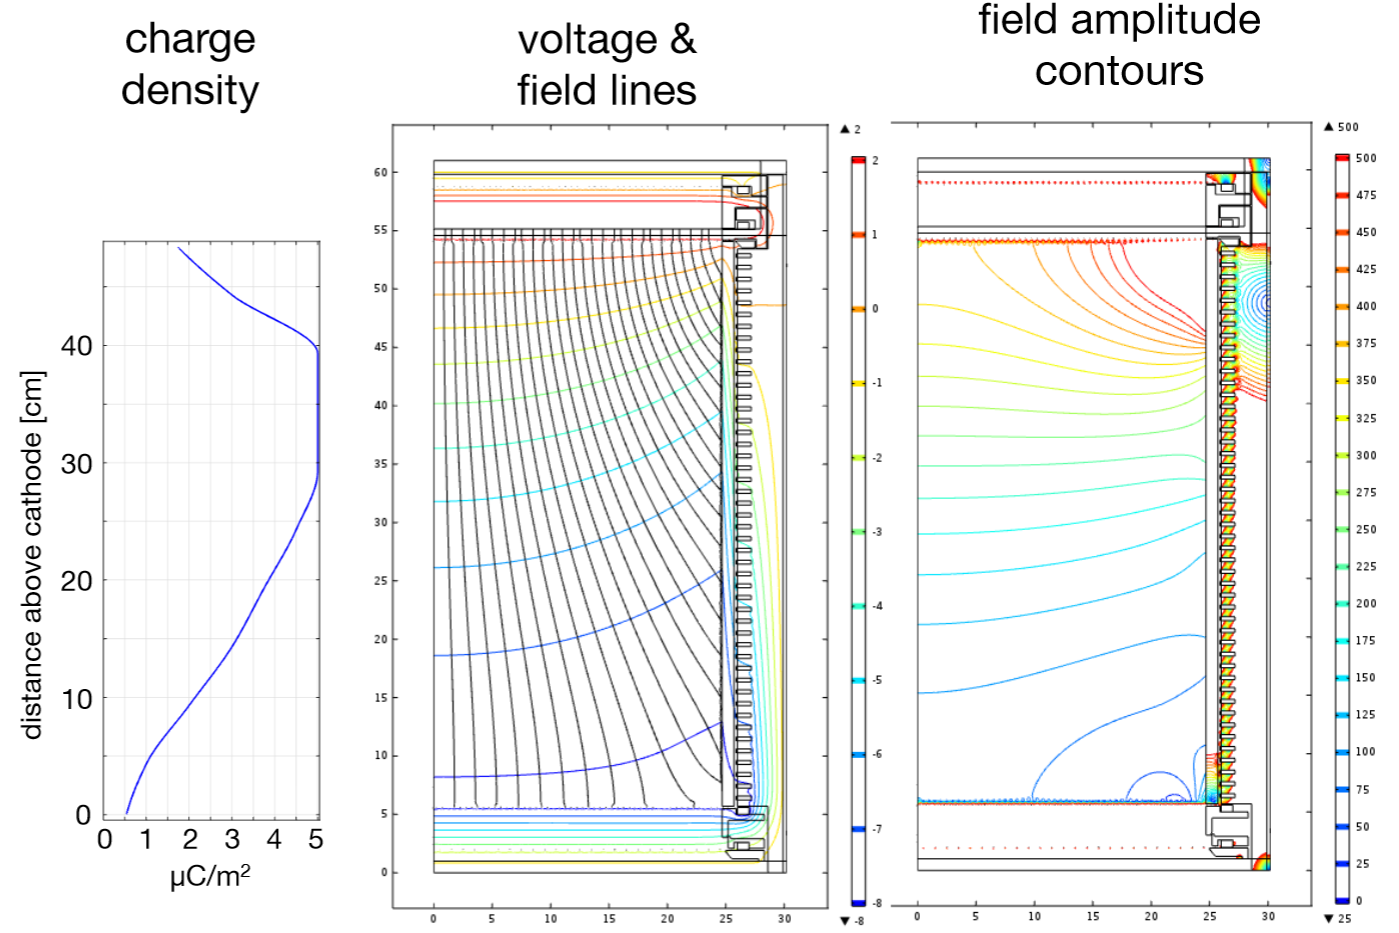
\includegraphics[scale=0.4]{Run04Corrections/Sep2014_Field_Detailed.png}
\captionof{figure}{The results of the preliminary field mapping technique for September 2014.\cite{ScottsMap} }
\label{fig:ScottsFieldMap}
\end{figure}

\subsubsection{Complications Arising from the Run4 Electric Field} \label{section:NEST}

The nonuniform electric field in Run4 introduces a number of complications to the data.  The most obvious of these complications is a radial squeezing in position reconstruction.  As charge from an event drifts upward it is pushed toward smaller radii due to the radial component of the electric field.  As a result, the XY position of the S2 signal is significantly separated from the XY position of the event itself.  Due to their longer drift time, this effect is more pronounced in events from the bottom of the detector (Figure \ref{fig:ScottsFieldMap2}). We use our field models to reconstruct the position of the events more accurately, but since signal corrections are produced using the uncorrected coordinates of the S2 signals, a discussion of this technique is outside of the scope of this chapter~\cite{PositionRecon}.

The variation of the electric field complicates the Z position reconstruction of events as well.  As the field evolves over time the drift velocity throughout the detector changes.  As a result, the mapping of drift time in $\mu$s to physical position in mm is no longer constant in time or space. Note that in particular this introduces complications when defining the electron lifetime in Run4, since the drift time to mm mapping is no longer one-to-one and the electron capture cross section is dependent on the drift-velocity.  We can use our field models to map the uncorrected drift time position to the physical position of events, but since the corrections are produced in the drift time coordinate system, details of this process are again out of the scope of this chapter~\ref{section:DescribingField}.  

A more subtle complication introduced by the nonuniform electric field lies in the recombination physics that occurs during a recoil event.  During a recoil, ionizing radiation produces both ionization and excitation of the xenon atoms.  The xenon excimers (Xe$_2^*$) produce scintillation light as they return to the ground state, which we observe as our S1 signal. Some of the electrons produced during ionization escape the location of the event, drift to the top of our detector, and produce our S2 signal.  The electrons that do not escape the event recombine with the ionized xenon atoms in a process called recombination, producing additional xenon excimers that contribute to the S1 signal.  Recoil events which occur in a low field region of the detector have a higher chance to recombine, and therefore produce more S1 signal and less S2 signal than an equivalent event in a high field region.  Complicating this matter further, the strength of this effect is dependent on the energy of the event and whether the event is an electron recoil (ER) or a nuclear recoil (NR) (Figure \ref{fig:LYQY}).  This source of pulse area variation in space and time will be referred to as "field effects" throughout this chapter.  This means that any pulse area corrections which are based solely on the spatial dependence of $^{83m}$Kr data, as was done in Run3, are no longer valid for ER or NR events in the WIMP search energy range.  In a uniform field, such as the Run3 data, detector response corrections can be derived by demanding that $^{83m}$Kr data be independent of position and time.  In a non-uniform field, this is not a valid strategy, because the field effects reflect a genuine variation in light and charge yields, rather than an artifact of detector response.

\begin{figure}[!h]
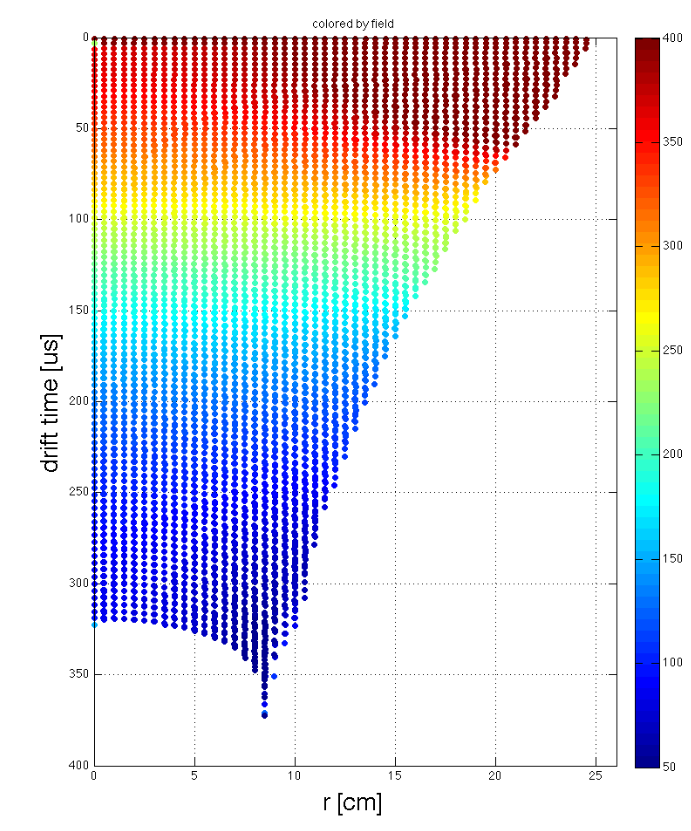
\includegraphics[scale=0.5]{Run04Corrections/Sep2014_Field.png}
\captionof{figure}{The reconstructed distribution of events resulting from the field map in Figure \ref{fig:ScottsFieldMap}.  Each point in the figure was placed on a uniform grid and allowed to drift to the liquid surface, where the final radius is measured.  The color of each point indicates the strength of the electric field in this "uncorrected" XY coordinate system.  This simulation reproduces the distribution of events seen in data from September 2014.   \cite{ScottsMap} }
\label{fig:ScottsFieldMap2}
\end{figure}

\begin{figure}[!h]
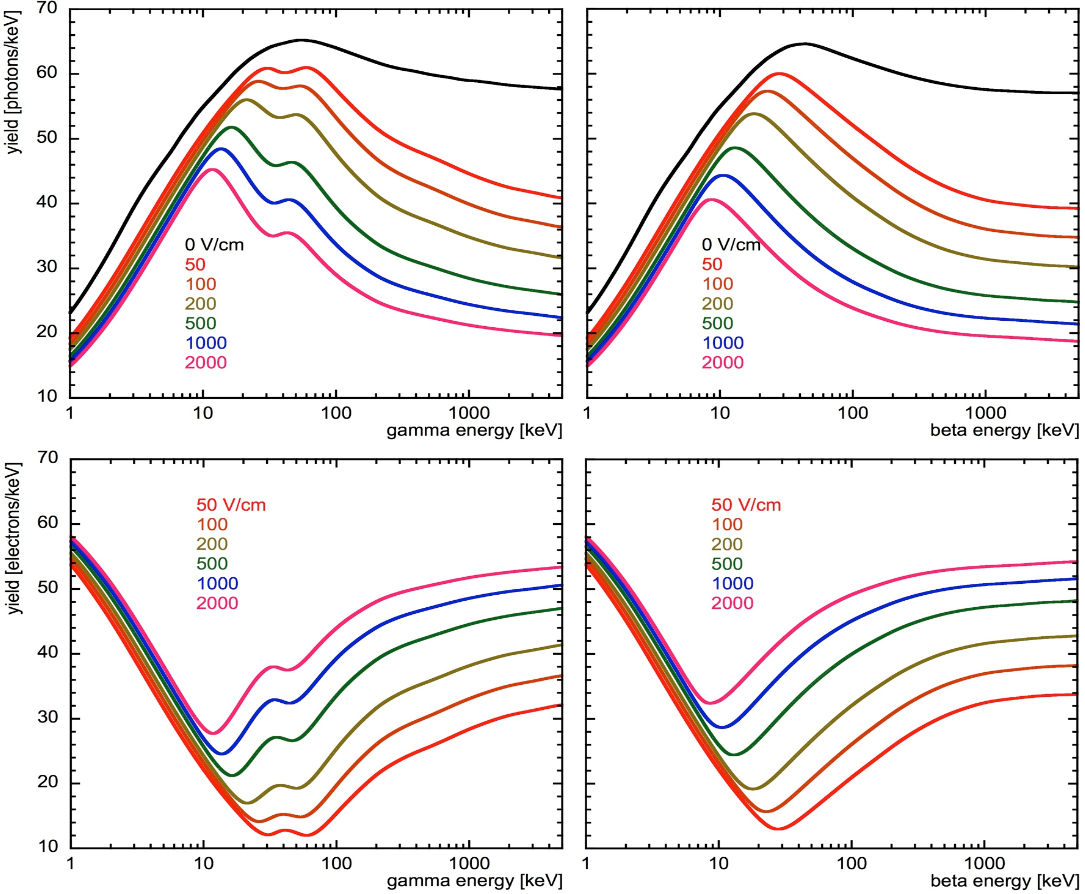
\includegraphics[scale=0.4]{Run04Corrections/Recomb.png}
\captionof{figure}{Predictions from NEST for the light yield (top row) and charge yield (bottom row) of electron recoil event from gamma ray interaction (left column) and beta particle interaction (right column).  Field values are indicated by the colored lines.  Light yield and charge yield have less dependence on the field strength for lower energy events.  \cite{RecombSource} }
 \label{fig:LYQY}
\end{figure}


\subsubsection{The Goal of KrypCal in Run4} \label{section:goal}

In Run4 the pulse area corrections must account for field effects as a function of time, space, energy, and recoil type.  Since the recoil type of an event in WIMP search data is unknown with exact certainty, and the energy of an event in WIMP search data is unknown prior to pulse area corrections being applied, it is not possible to remove the spatial and time dependence induced by the field effect in our data.  Instead, we seek to separate the field effect from the detector inefficiency effects at the known energy and recoil type of $^{83m}$Kr, so that we can extract detector efficiency corrections that are applicable to all events.  This separation must be performed at all points in time due to the time dependence of the electric field.  To accomplish this we will relate the strength of the field effects in the S1 and S2 pulse areas of $^{83m}$Kr calibration data to the ratio of the two S1 pulses (referred to as S1a and S1b) generated during the $^{83m}$Kr decay.  This ratio should be strongly correlated to the strength of the electric field effect, since the two $^{83m}$Kr decays have different energies (32.1 keV for S1a and 9.4 keV for S1b) and are therefore effected by the electric field by different amounts.  Note that corrections which perfectly separate field effects from detector inefficiency effects in this manner, and only correct for the latter, will have a spatial and time dependence left in the S1 and S2 signals, but not in the energy spectra from any source, regardless of energy or recoil type.

\subsection{Measuring Electric Field Effects in $^{83m}$Kr Data}

\subsubsection{General Strategy for Measuring the Field Effect} \label{section:GenStrat}

Before providing detailed descriptions of the Run4 corrections process, we will first discuss the general strategy for measuring and separating the electric field effect in $^{83m}$Kr calibrations.  First, we measure the electric field in the detector at a particular point in time, using the methods described in section \ref{section:DescribingField}. Due to their high statistics, we choose data sets in September 2015 for this purpose. We would like to use this field map in conjunction with NEST to remove the field effects in the $^{83m}$Kr data directly before measuring detector inefficiency effects.  Unfortunately, due to the complicated nature of the $^{83m}$Kr decay (detailed in Section \ref{KrSource}) NEST does not accurately simulate $^{83m}$Kr data.  Instead we turn to CH$_3$T data, which NEST has been tuned to simulate extremely well.  

After using NEST to determine and remove the strength of the field effects in CH$_3$T data, we measure the residual pulse area variation in the S2 signal and produce corrections for these effects, which, since the field effects have been removed, are due to detector inefficiencies alone.  The same process can not be repeated for the S1 signal, since the maximum of the CH$_3$T S1 spectrum falls below the detector threshold.  These S2 corrections are equivalent to the Run3 S2 corrections which were obtained directly from $^{83m}$Kr data when there was no significant field variation.  Next, we apply the detector inefficiency corrections to contemporaneous $^{83m}$Kr data.  At this point, any residual pulse area variation in the $^{83m}$Kr S2 signal is due to field effects alone.  We measure the strength of the field effects by fitting Gaussian distributions to the inefficiency corrected $^{83m}$Kr S2 signal over a three dimensional map, choosing the ratio S2(XYZ)/S2(Center) as the figure of merit for the strength of the field effect.  At the same time we measure a three dimensional map of the $^{83m}$Kr S1a/S1b ratio.  Relating these two maps allows us to determine the strength of the field effect on $^{83m}$Kr S2 data taken at any time or location by simply measuring the $^{83m}$Kr S1a/S1b ratio. 

Three approaches have been taken to measure the relationship of the field effect in inefficiency corrected $^{83m}$Kr S1 data, as measured by S1(XYZ)/S1(Center), to the $^{83m}$Kr S1a/S1b ratio.  The first approach, in section \ref{section:S1relation}, converts the S2 field effect relationship to an S1 field effect relationship using the physics behind recombination.  In section \ref{MatthewsIdea} we use the expected light yield of the $^{83m}$Kr 31.2 keV decay as a function of electric field to measure detector inefficiency effects and separate them from the field effect we want to measure.  The final approach, in section \ref{section:S1relation2}, takes advantage of the fact that the total combined energy of any event should remain insensitive to any recombination variation that arises from a non-uniform electric field.  In this method, we float the $^{83m}$Kr S1(XYZ)/S1(Center) to S1a/S1b relationship in a $\chi^2$ fit.  Within the fit we remove the field effect in both the S1 and S2 $^{83m}$Kr data (using the floated relationship for the S1 field effect), produce inefficiency-only corrections from the data, and then evaluate the corrected $^{83m}$Kr and CH$_3$T energy spectra.  The  S1(XYZ)/S1(Center) to S1a/S1b relationship which produces the minimum $\chi^2$ between the observed and expected energy spectra is chosen as the correct relationship.

Once the field induced S2(XYZ)/S2(Center) to S1a/S1b relationship and the field induced S1(XYZ)/S1(Center) to S1a/S1b relationship have been determined, they can be used in $^{83m}$Kr data sets from any time to remove the field effects in the $^{83m}$Kr data via mapping the S1a/S1b ratio.  Once the field effects are removed the residual S1 and S2 variation in the $^{83m}$Kr can be used to calculate pulse area corrections based on detector inefficiencies alone.  In the following sections we will describe each step of the process outlined above in detail.

\subsubsection{Measuring Detector Inefficiency Corrections with CH$_3$T}

Before measuring detector inefficiency corrections in CH$_3$T we must first remove the field effects from the data.  We use data from the September 2015 CH$_3$T calibration due to its high statistics.  A simple box cut of (630 $\leq$ uncorrected S2 $\leq$ 14000) and (uncorrected S1 $\leq$ 125) is used to select CH$_3$T events from the data set, as shown in Figure \ref{fig:TritBoxCut}. The electric field at the location of each CH$_3$T event is estimated by interpolating the RvZ field map (described in section \ref{section:DescribingField}) from September 2015.  A cubic interpolation is used for events which fall within the bounds of the field map, and a nearest neighbor extrapolation is used for events which fall outside of the bounds.   Note that we choose to use preliminary 2D field maps from Figure~\ref{fig:ScottsFieldMap2} for this work because interpolating and extrapolating is simplified in a two dimensional map, because the preliminary field maps varies more smoothly in space due to the smooth charge density distribution in the simplified field model, and because the final field models were not finalized at the time of this work.  

\begin{figure}[!h]
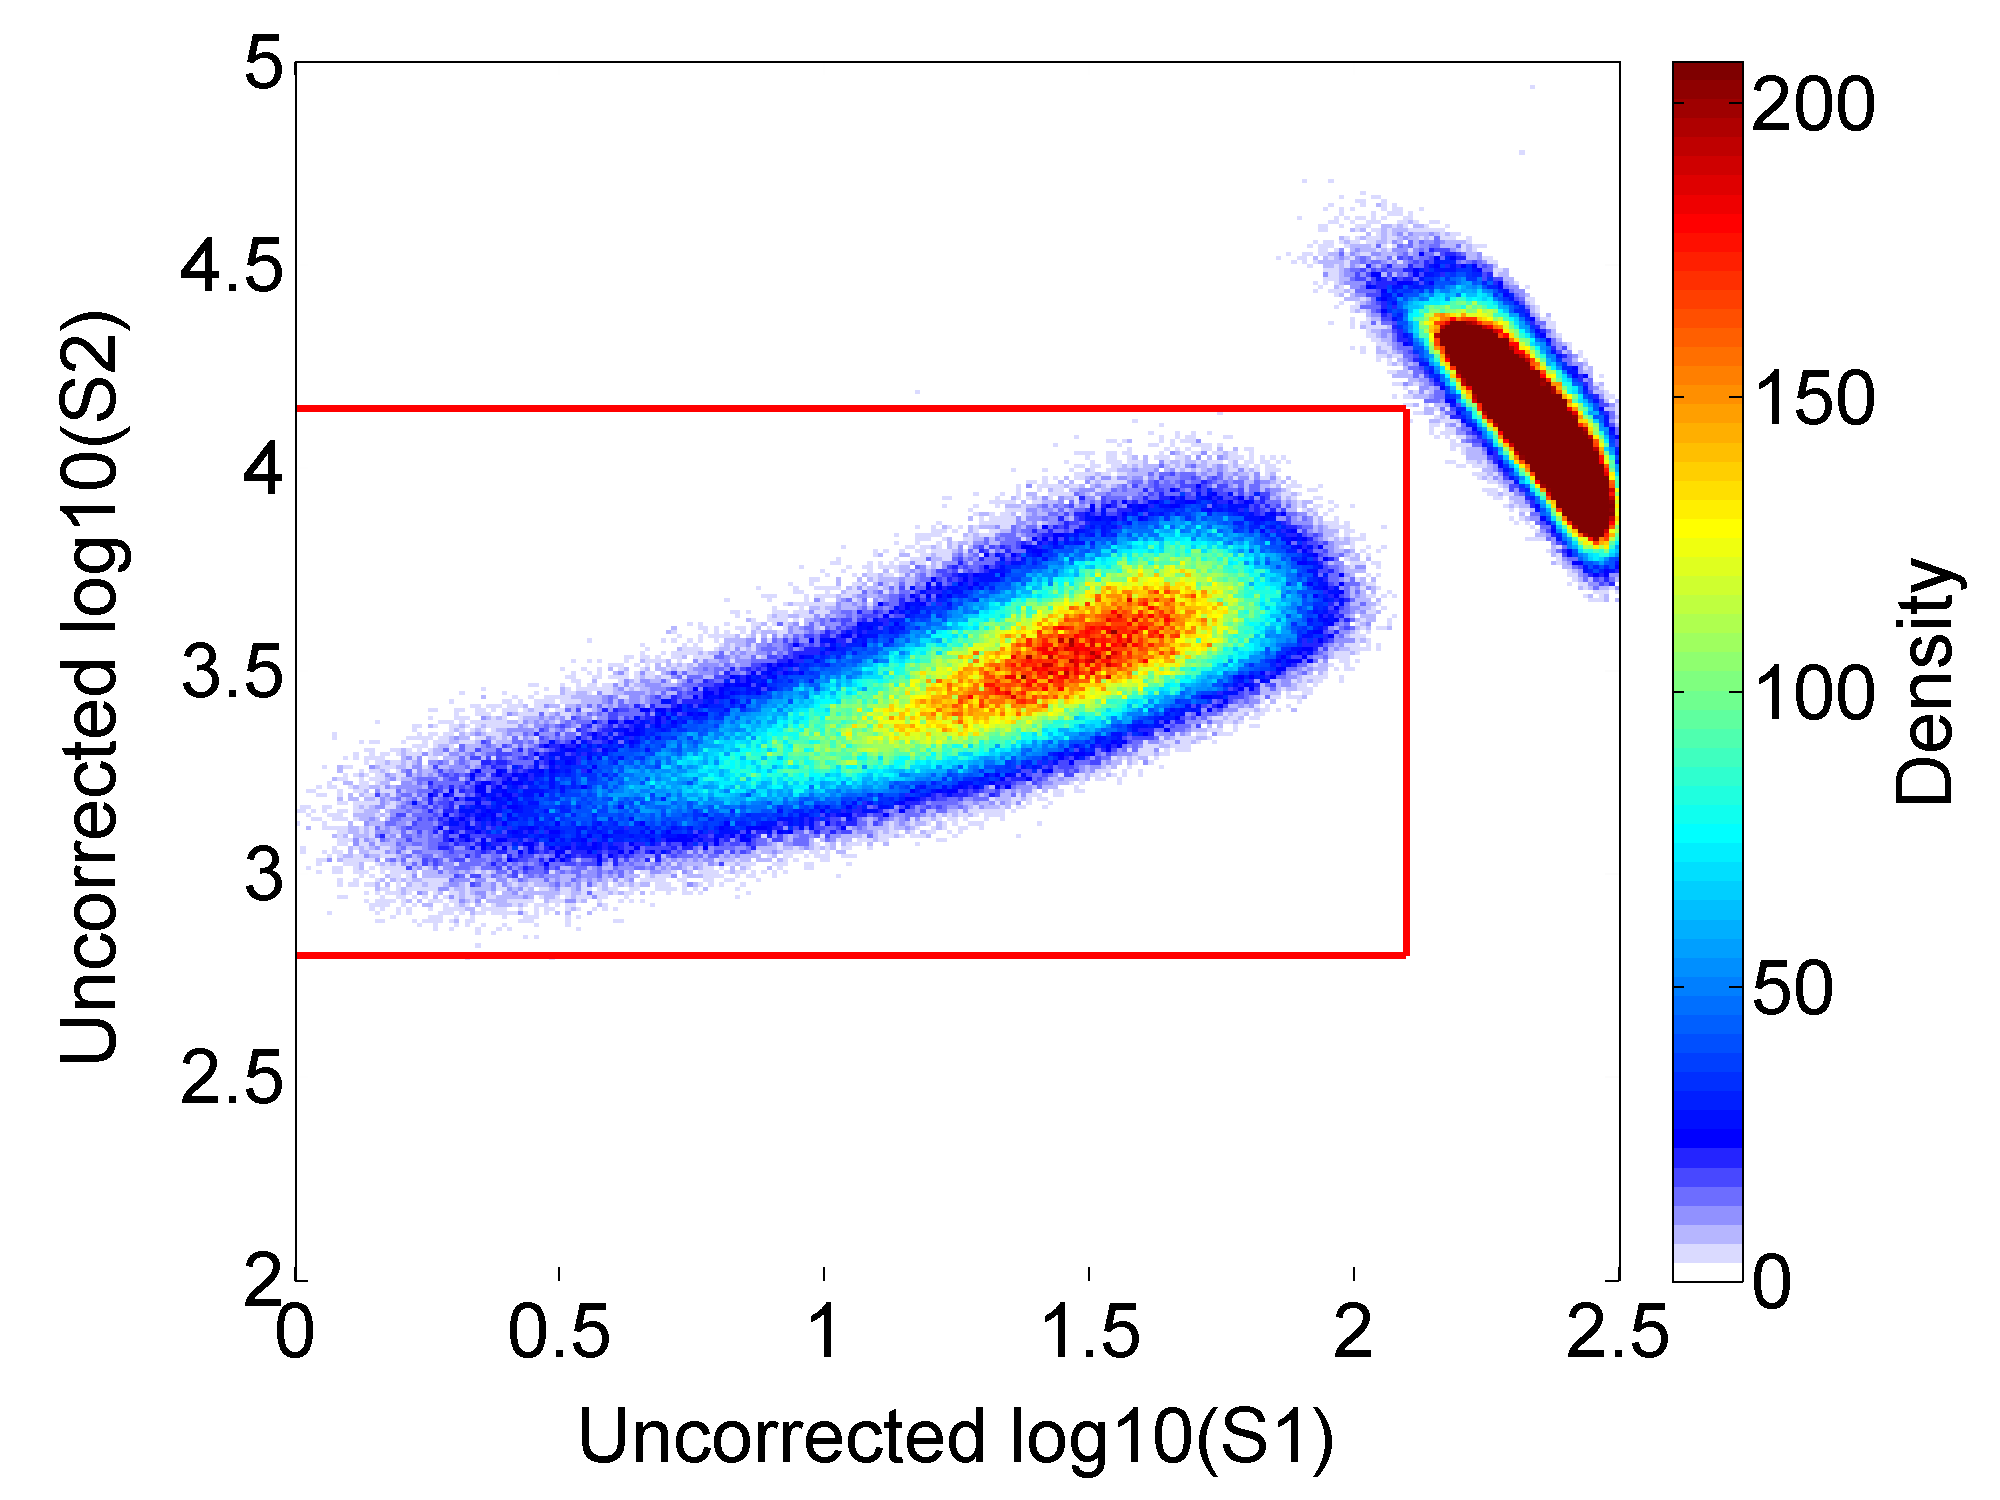
\includegraphics[scale=0.6]{Run04Corrections/TritiumDetectorInefficiency_Cuts.png}
\captionof{figure}{Density plot of uncorrected S1 versus uncorrected S2 from the September 2015 CH$_3$T calibration.  The red lines indicate the box cut used to select CH$_3$T events.  The dense population to the right of the box cut is $^{83m}$Kr which is present in the data set and excluded from the box cut.}
 \label{fig:TritBoxCut}
\end{figure}


Once the field strength at the location of a particular event is determined it is converted to a measurement of the recombination for each event using the following equation from NEST. (Figure \ref{fig:RecombMap}) 
\begin{align}
N_q &= \frac{E}{0.0137} \label{NqEq} \\
N_{ion} &= \frac{N_q}{1+\alpha} \label{NionEq} \\
R &= 1-\mbox{ln} \left( \frac{1+(\frac{TI*N_{ion}}{4})}{(\frac{TI*N_{ion}}{4})} \right)
\end{align}
where $E$ is the energy of the event in keV, $N_q$ is the number of quanta, $N_{ion}$ is the number of ions, $\alpha$ is the exciton to ion ratio (assumed to be 0.11), $TI$ is the Thomas-Imel Box parameter, and $R$ is the recombination probability.  Since we do not know the energy of the event ahead of time (since we do not have working corrections at this point) we assume the most probably energy from the CH$_3$T energy spectrum, which is 2.5 keV.  We are mainly interested in fitting the maximum of the spectrum when measuring detector inefficiency corrections, so the fact that this recombination estimate for higher energy CH$_3$T events may be off by up to a factor of 2.5 is not concerning.  

\begin{figure} [!h]
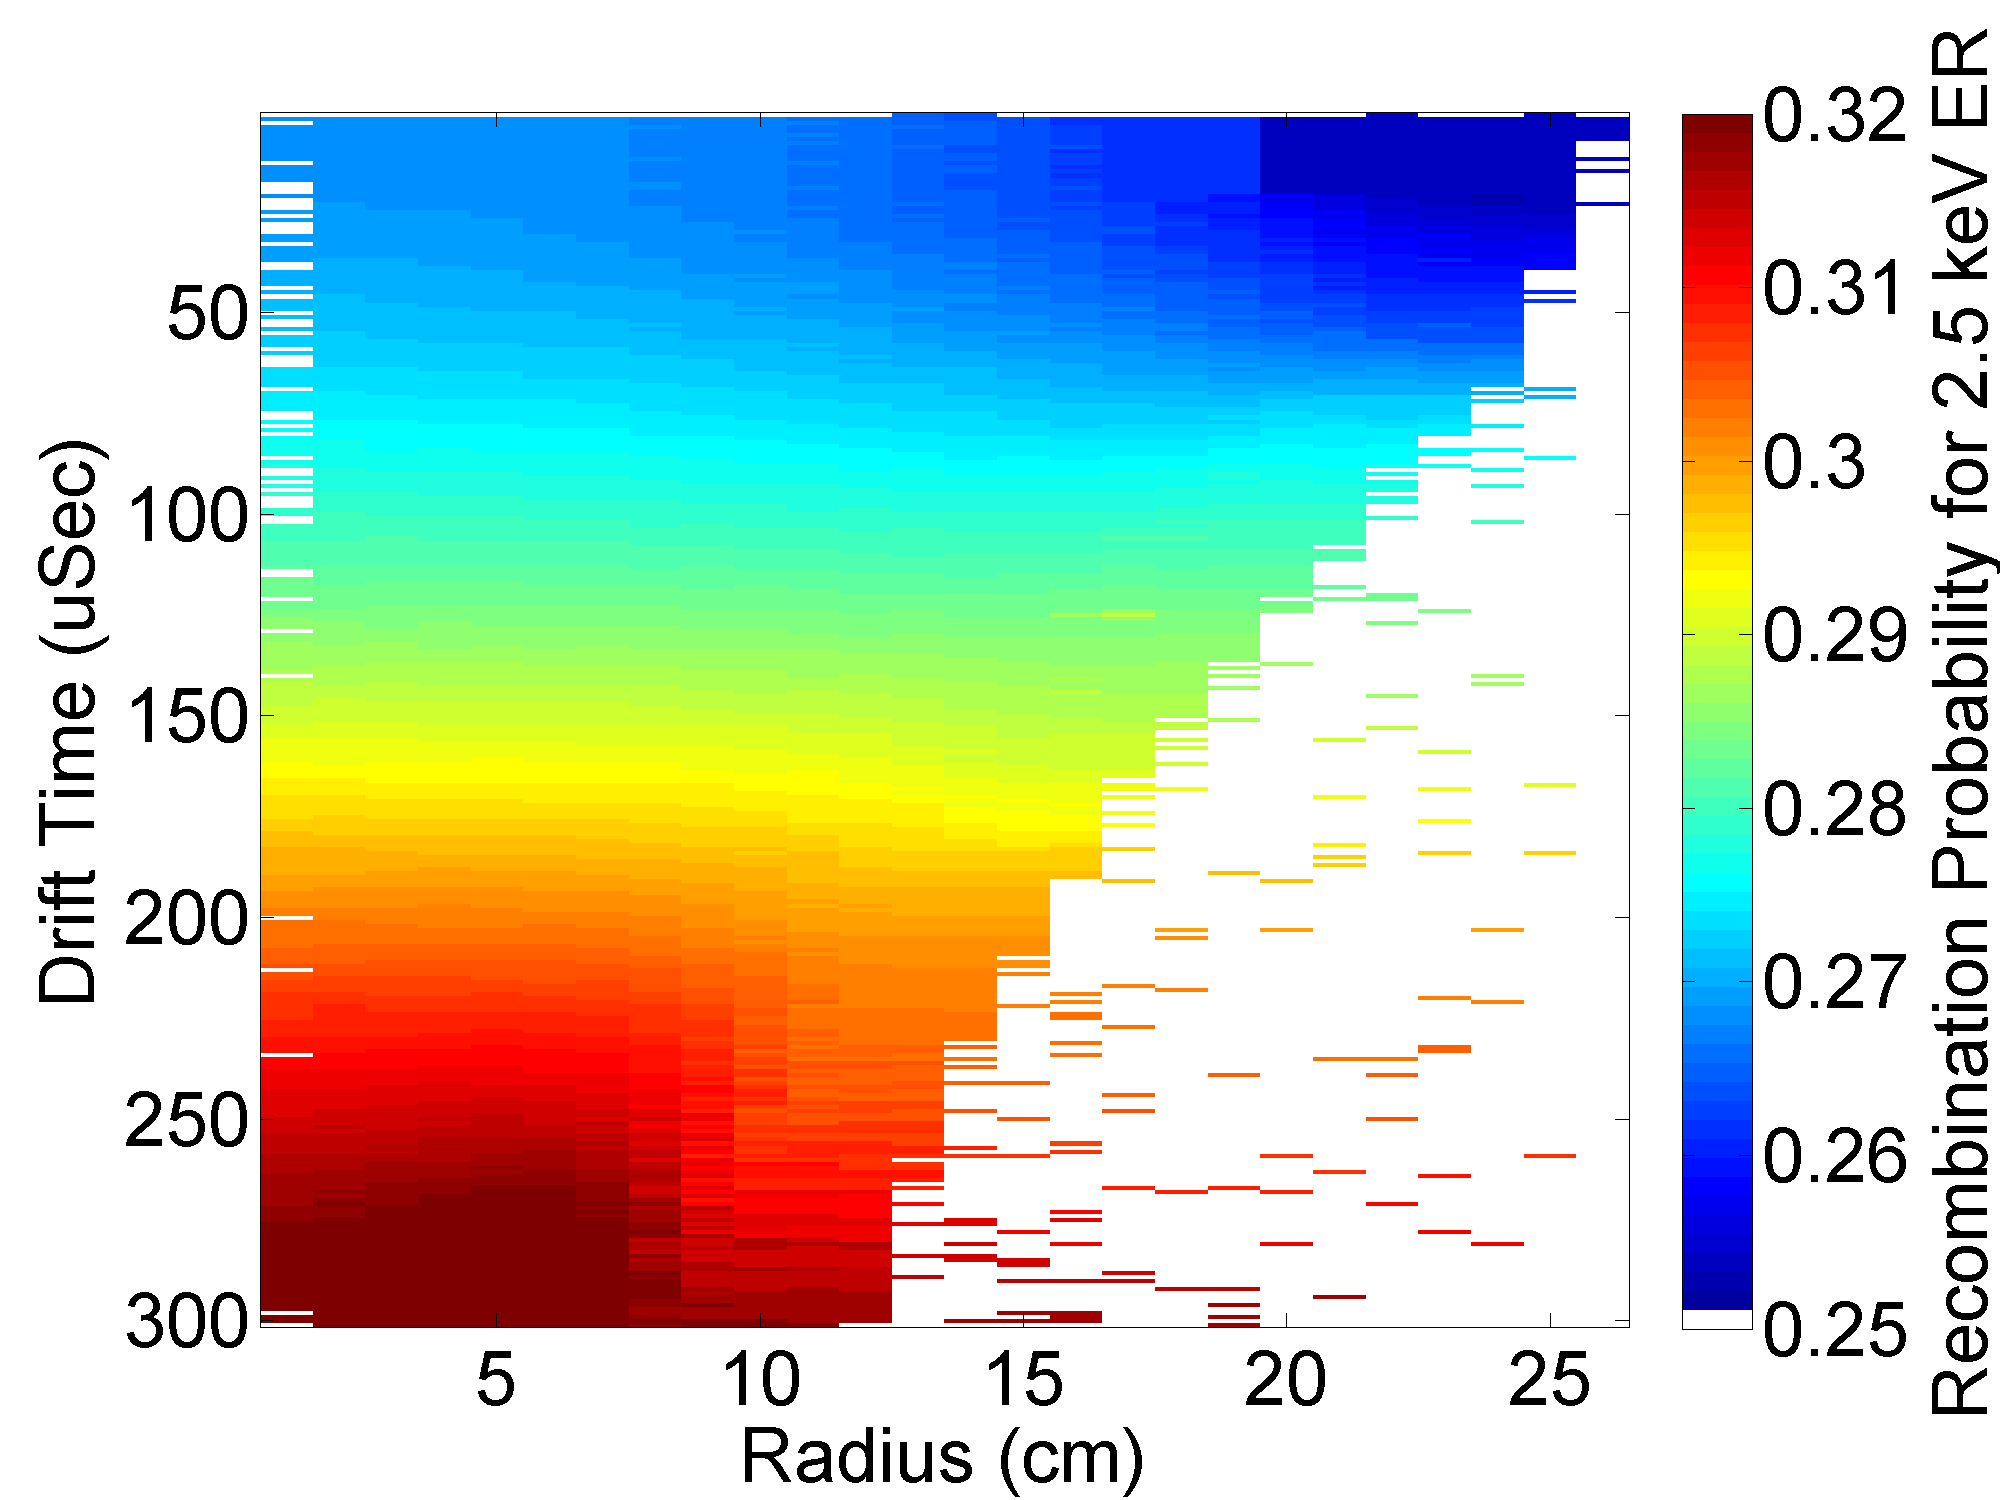
\includegraphics[scale=0.5]{Run04Corrections/TritiumDetectorInefficiency_RecombMap.png}
\captionof{figure}{Two dimensional map of the recombination probability for a 2.5 keV ER based on the September 2015 RvZ electric field map and NEST. Radius is uncorrected, as observed at the anode.}
\label{fig:RecombMap}
\end{figure}


A normalization factor $N_{photon-center}/N_{photon}$ for the S1 signal is determined by calculating the number of photons produced in events at the center of the detector, and the number of photons produced in a particular event by using
\begin{equation}
N_{photon} = N_q\frac{\alpha}{1+\alpha} + N_{ion}R
\end{equation}
Since we assumed a value of 2.5 keV for all events, $R$ only has a dependence on the estimated field strength, and therefore the normalization constant only has a dependence on the estimated field strength at each location in the detector as well.  Similarly, we determine a normalization factor $N_{elec-center}/N_{elec}$ for the S2 signal by calculating the number of electrons at the center of the detector and the number of electrons for a particular event by using the equation
\begin{equation}
N_{elec}=N_q-N_{photon}
\end{equation}
which again is only dependent on the estimated field strength at each location in the detector.  We simply multiply the raw S1 and S2 signals by these normalization factors to remove the field effects from the CH$_3$T.  For clarity, we define the field effect removed S1 and S2 signals as S1$_F$ and S2$_F$, respectively, where the subscript $F$ stands for "field corrected".   
\begin{align}
S2_F &=S2 \left( \frac{N_{elec-center}}{N_{elec}} \right) \\
S1_F &=S1 \left( \frac{N_{photon-center}}{N_{photon}} \right)
\end{align}
Likewise, we define the detector inefficiency corrected S1 and S2 signals (with field effects still present) as S1$_E$ and S2$_E$, where the subscript $E$ stands for "efficiency corrected", and the detector inefficiency corrected and field effect removed S1 and S2 signals as S1$_{EF}$ and S2$_{EF}$, where the subscript $EF$ stand for "efficiency and field corrected" . 

After removing the field effects from the CH$_3$T data we are ready to measure the residual spatial pulse area variation due to detector inefficiencies alone.  We first measure the Z dependence of the S2$_F$ pulse area by slicing the detector into drift time bins of 10 $\mu$s width.  This is intended to correct for the effects of charge attenuation in the LXe. A Landau distribution is fit to the S2$_F$ spectrum of each bin to determine the location of the spectra maximums. (Figure \ref{fig:LandauPlot})  Polynomial and skew Gaussian fits have also been used to determine the maximums with consistent results between all three methods.  A cubic interpolation is used to determine the S2$_F$ Z dependence between each drift time bin, and a linear extrapolation based on the first and last 20\% of Landau distribution data points is used to determine the S2$_F$ Z dependence above and below the span of the drift time bins  (10 to 330 $\mu$s).  A detector inefficiency correction for the Z direction is defined by taking the ratio of the S2$_F$ pulse area at a height of 4 $\mu$s (just below the liquid surface) to the S2$_F$ pulse area as described in the equation
\begin{equation}\label{s2zcorr_eq}
\mbox{S}2_{\mbox{z-efficiency-correction}} = \frac{S2_F(z=4)}{S2_F(z)}.
\end{equation} 


\begin{figure} [!h]
\centering
\subfloat{{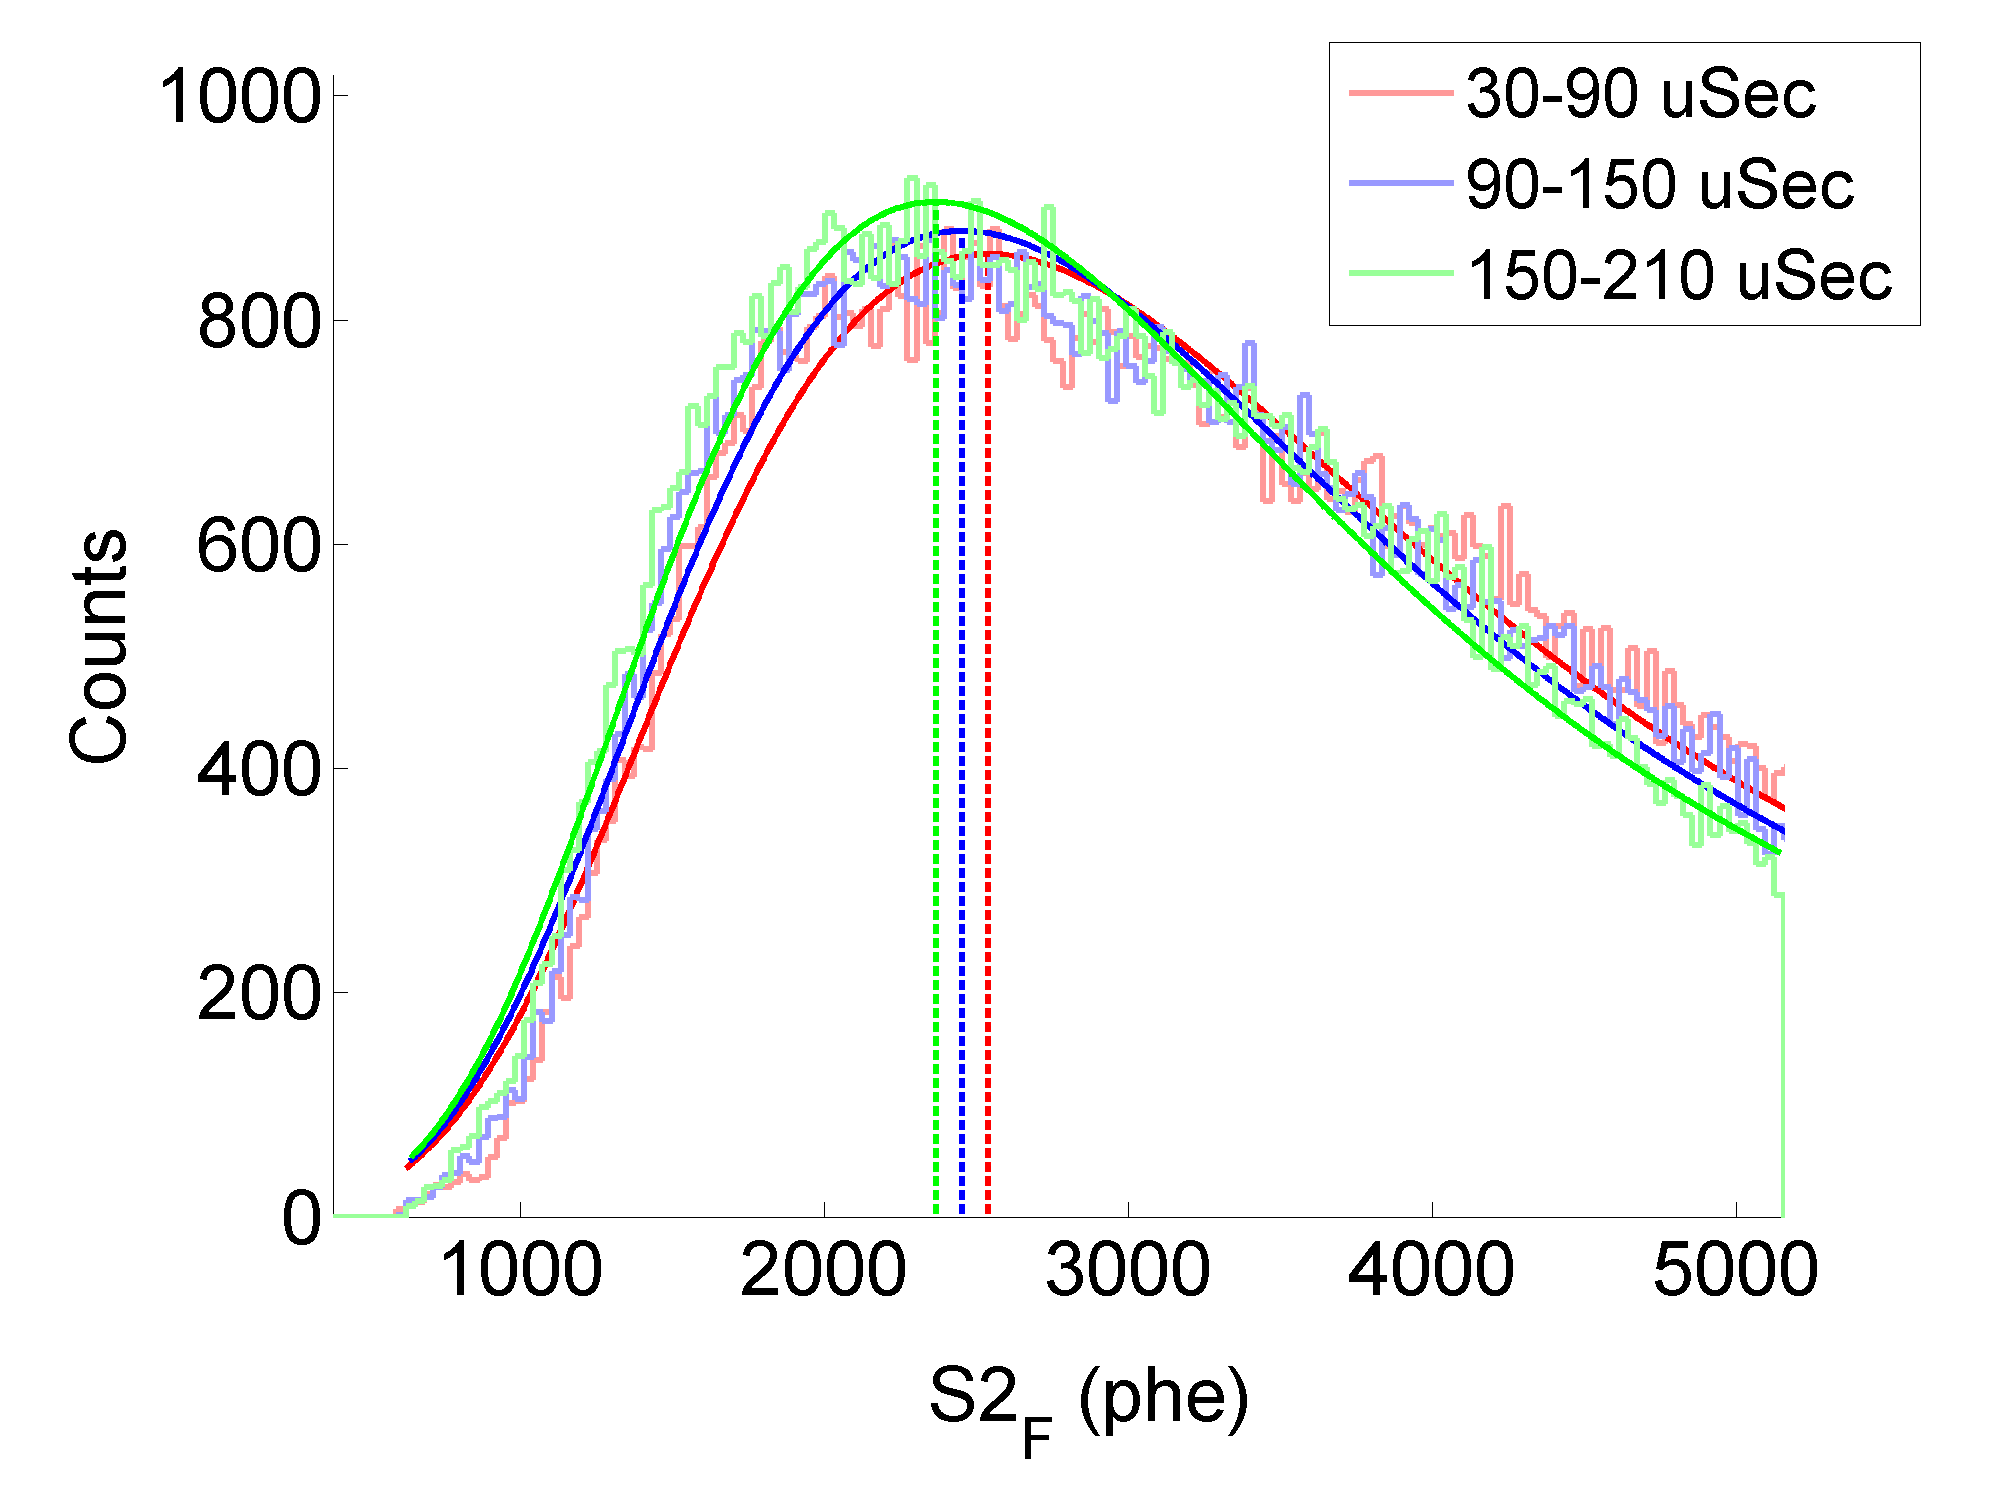
\includegraphics[width=6.7cm]{Run04Corrections/LandauFits.png} }}
\qquad
\subfloat{{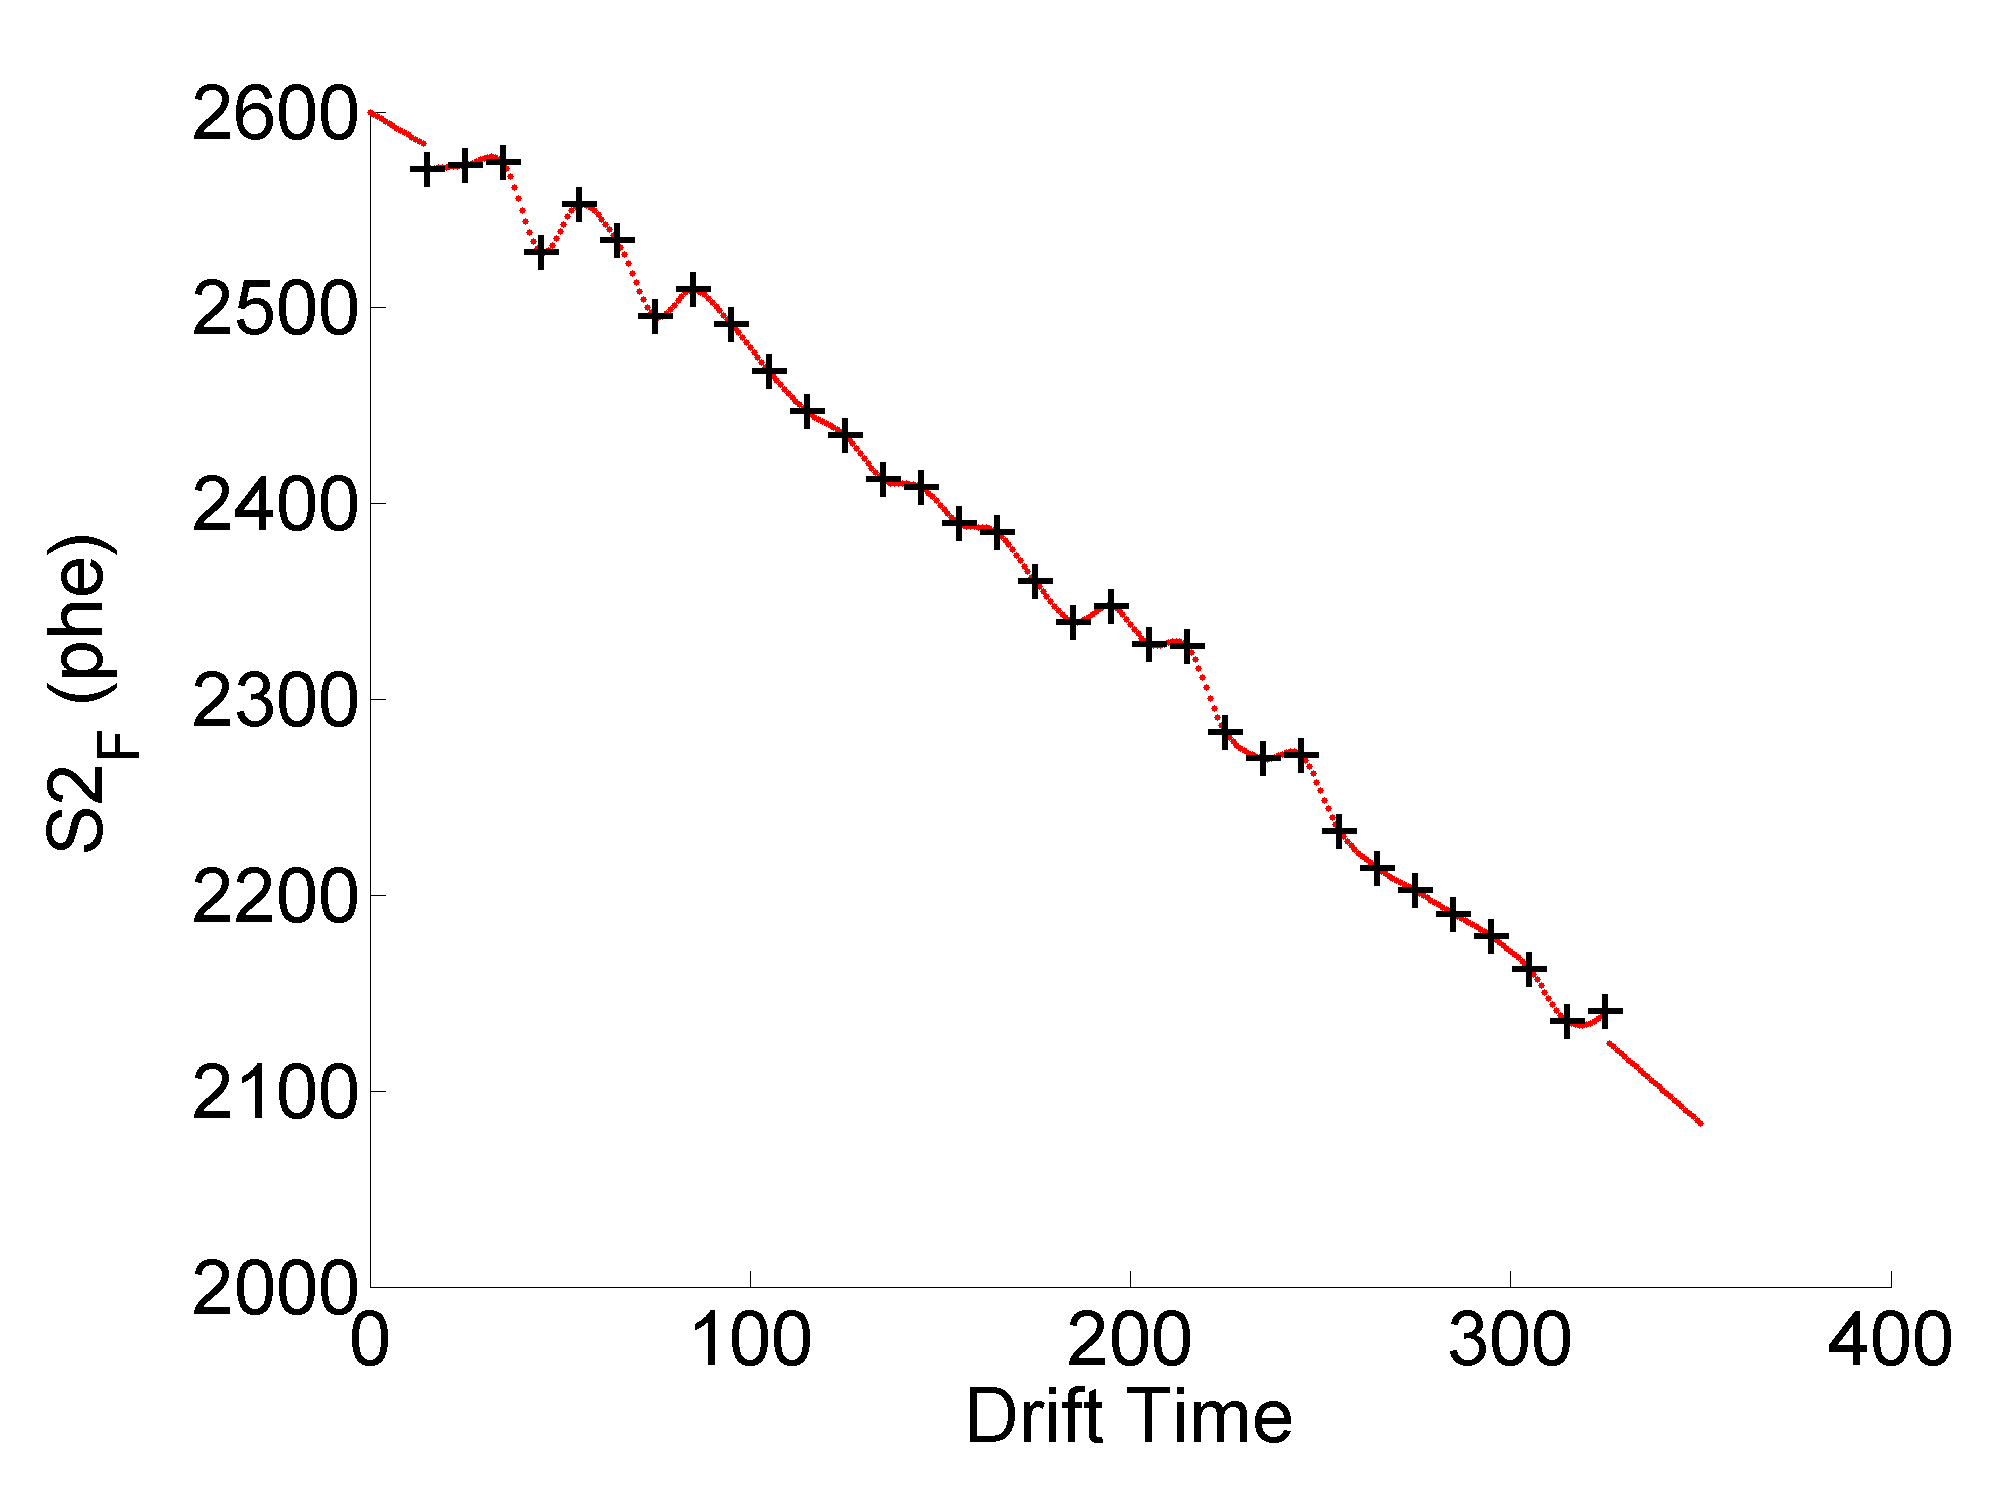
\includegraphics[width=6.7cm]{Run04Corrections/CH3T_S2_ZDep.png} }}
\captionof{figure}{ (Left) Landau distribution fits to the S2$_F$ data that are used to determine the drift time dependence of the S2$_F$ pulse area. For illustrative purposes, a drift time bin width of 60 $\mu$s was chosen for this plot. (Right) The Z dependence of the S2$_F$ pulse area after field effects are removed.  Black points indicate the maximum of Landau distribution fits for each drift time bin, and the red line indicate the spline interpolation and linear extrapolation of that data.  Data shown is from the September 2015 CH$_3$T calibration.}
\label{fig:LandauPlot}
\end{figure}

The XY dependence of the field removed S2$_F$ signal is found by dividing the Z inefficiency corrected (S2$_F \times \mbox{S}2_{\mbox{z-efficiency-correction}}$) data into two dimensional XY bins with lengths of 3 cm on each side, and then fitting Landau distributions to the data of each bin.  The maximum of the Landau distribution from each bin is used to construct an S2$_F$ XY dependence map, with a spline interpolation and extrapolation being used to determine the XY dependence between and outside of the bins. (Figure \ref{fig:TritXYDep}) A detector inefficiency correction for the XY direction is defined by taking the ratio of the z inefficiency corrected S2$_F$ pulse area at the center of the detector to the z inefficiency corrected S2$_F$ pulse area as a function of XY in cm, as shown below
\begin{equation}\label{s2xycorr_eq}
\mbox{S}2_{\mbox{xy-efficiency-correction}} = \frac{\mbox{S}2_{\mbox{z-efficiency-correction}}\times S2_F(x_c,y_c,z)}{\mbox{S}2_{\mbox{z-efficiency-correction}}\times S2_F(xyz)}.
\end{equation} 
where $x_c$ and $y_c$ are the x and y center of the detector in uncorrected coordinates determined by taking the average position of the CH$_3$T events in each direction.

\begin{figure}[!h]
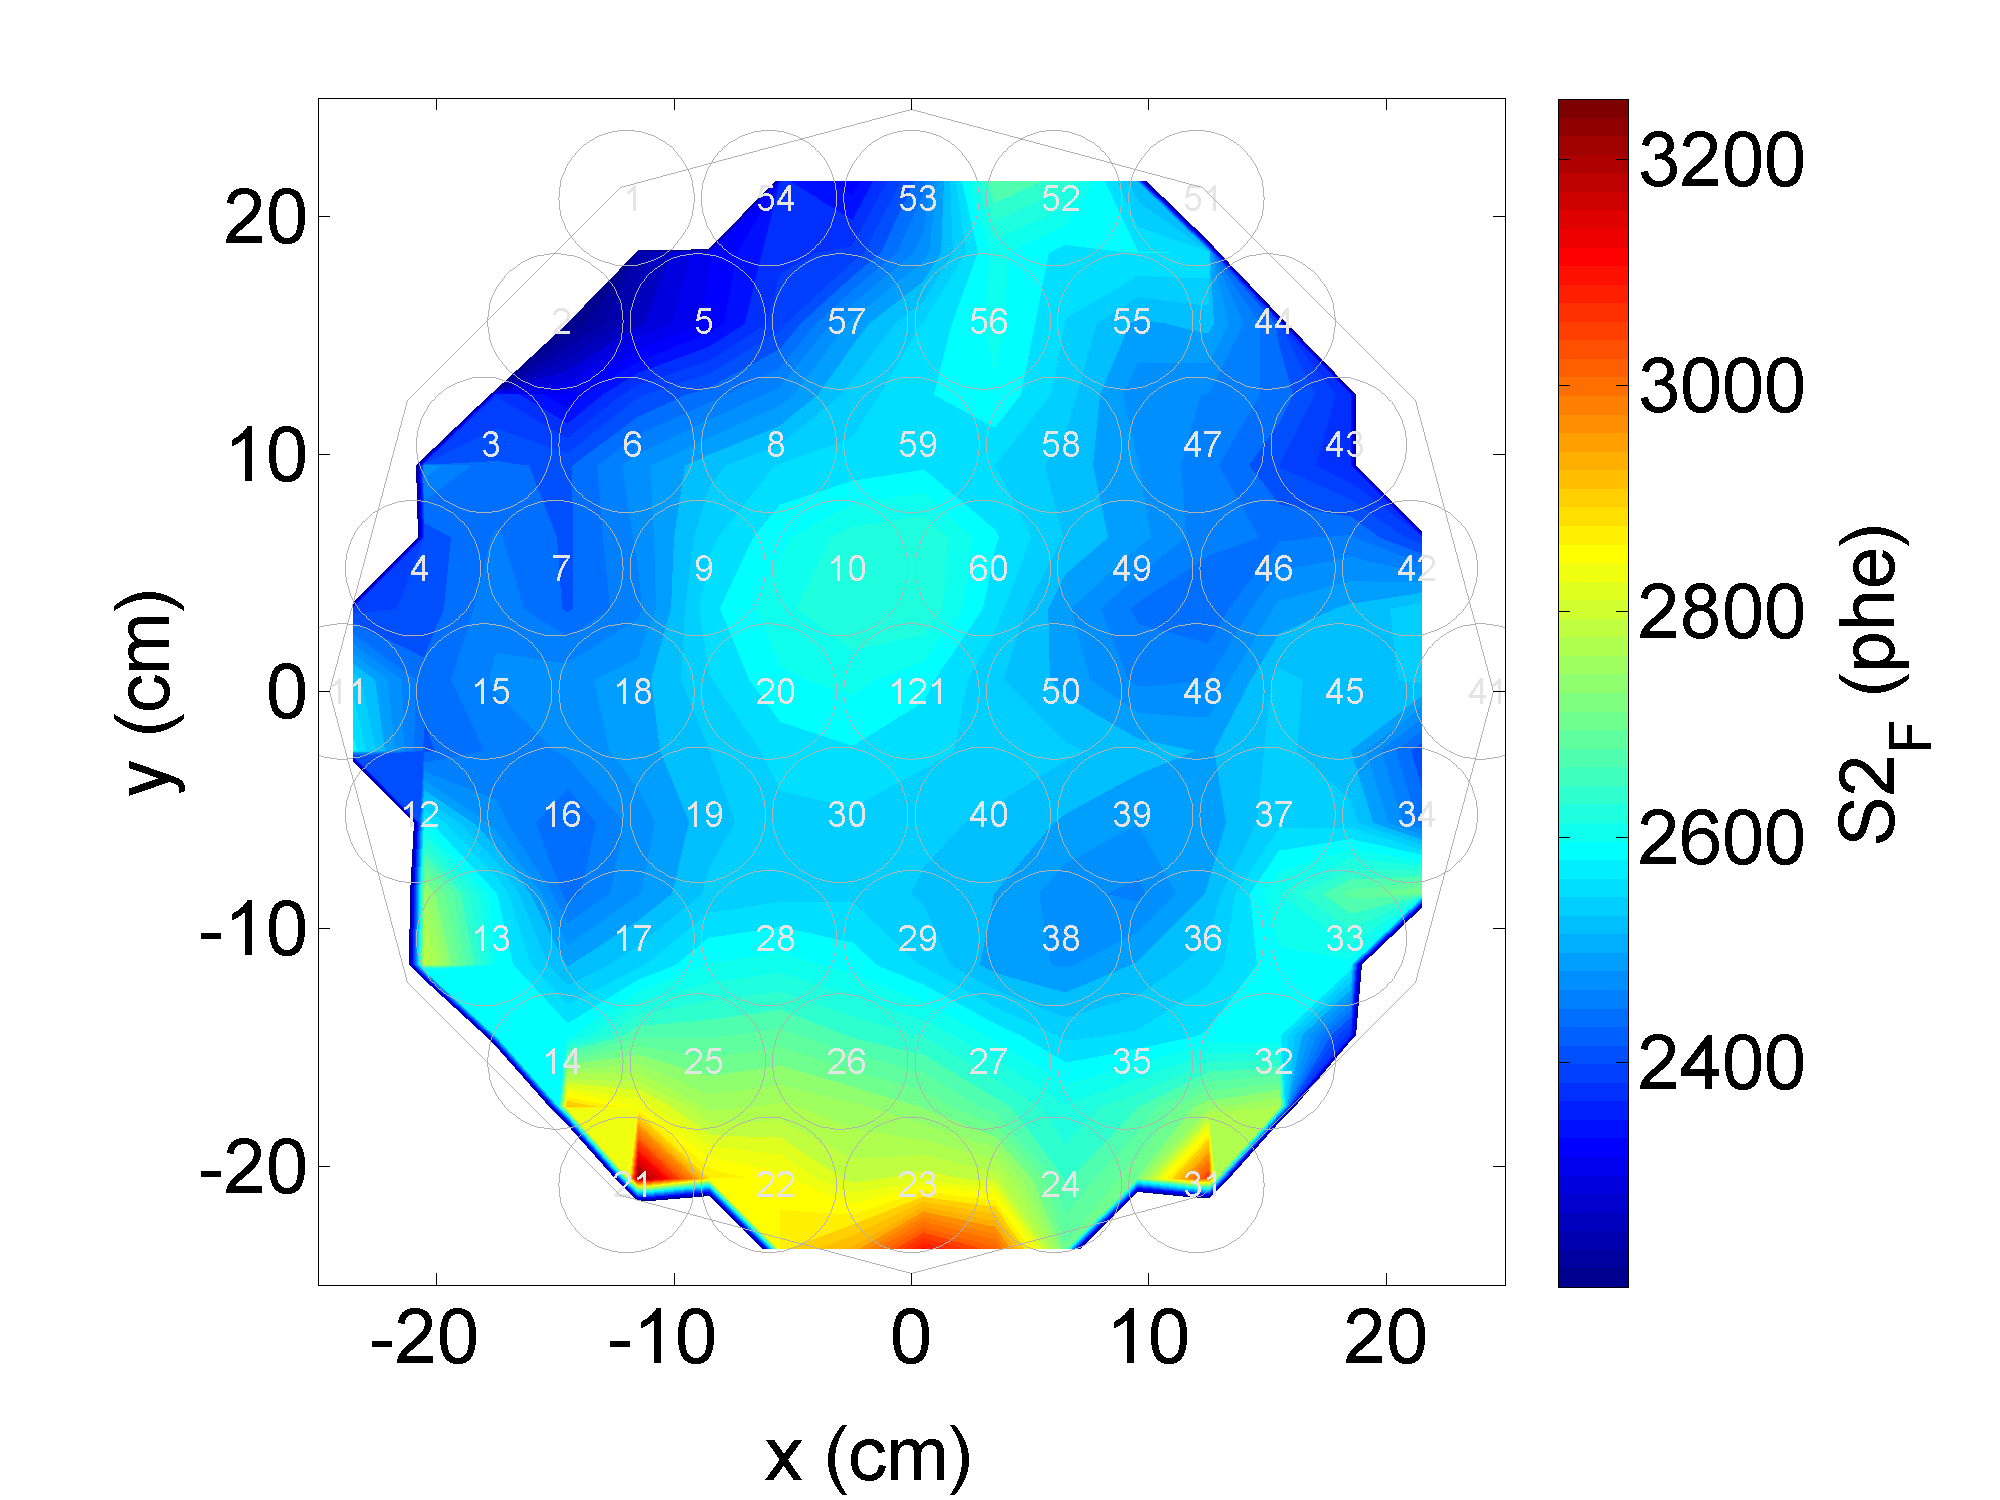
\includegraphics[scale=0.5]{Run04Corrections/CH3T_S2_XYDep.png}
\captionof{figure}{Two dimensional map of the XY dependence in CH$_3$T S2$_F$ data determine by fitting a Landau distribution to XY bins of the data and tracking the maximum of each fit.  Data is from the September 2015 CH$_3$T injection.}
 \label{fig:TritXYDep}
\end{figure}


Multiplying the raw S2 signal by both the Z and the XY correction factors results in an inefficiency corrected S2$_E$ signal (with field effects still present), and multiplying the field removed S2$_F$ signal by the correction factors results in a inefficiency and field corrected S2$_{EF}$ signal.
\begin{align}
S2_E &=S2 \times \mbox{S}2_{\mbox{xy-efficiency-correction}} \times \mbox{S}2_{\mbox{z-efficiency-correction}} \label{E_eq}\\
S2_{EF} &=S2_F \times \mbox{S}2_{\mbox{xy-efficiency-correction}} \times \mbox{S}2_{\mbox{z-efficiency-correction}} 
\label{EF_eq}
\end{align}

Unfortunately, we are unable to directly measure the detector inefficiency corrections for the S1 signal from CH$_3$T data, since the maximum of the S1 spectrum falls below the detector threshold and there are no discernible features to fit to (Figure \ref{fig:S1thresholded}). Instead, we will continue working with the S2 signal of our data and return to the issue of S1 corrections in sections \ref{section:S1relation} and \ref{section:S1relation2}.


\begin{figure}[!h]
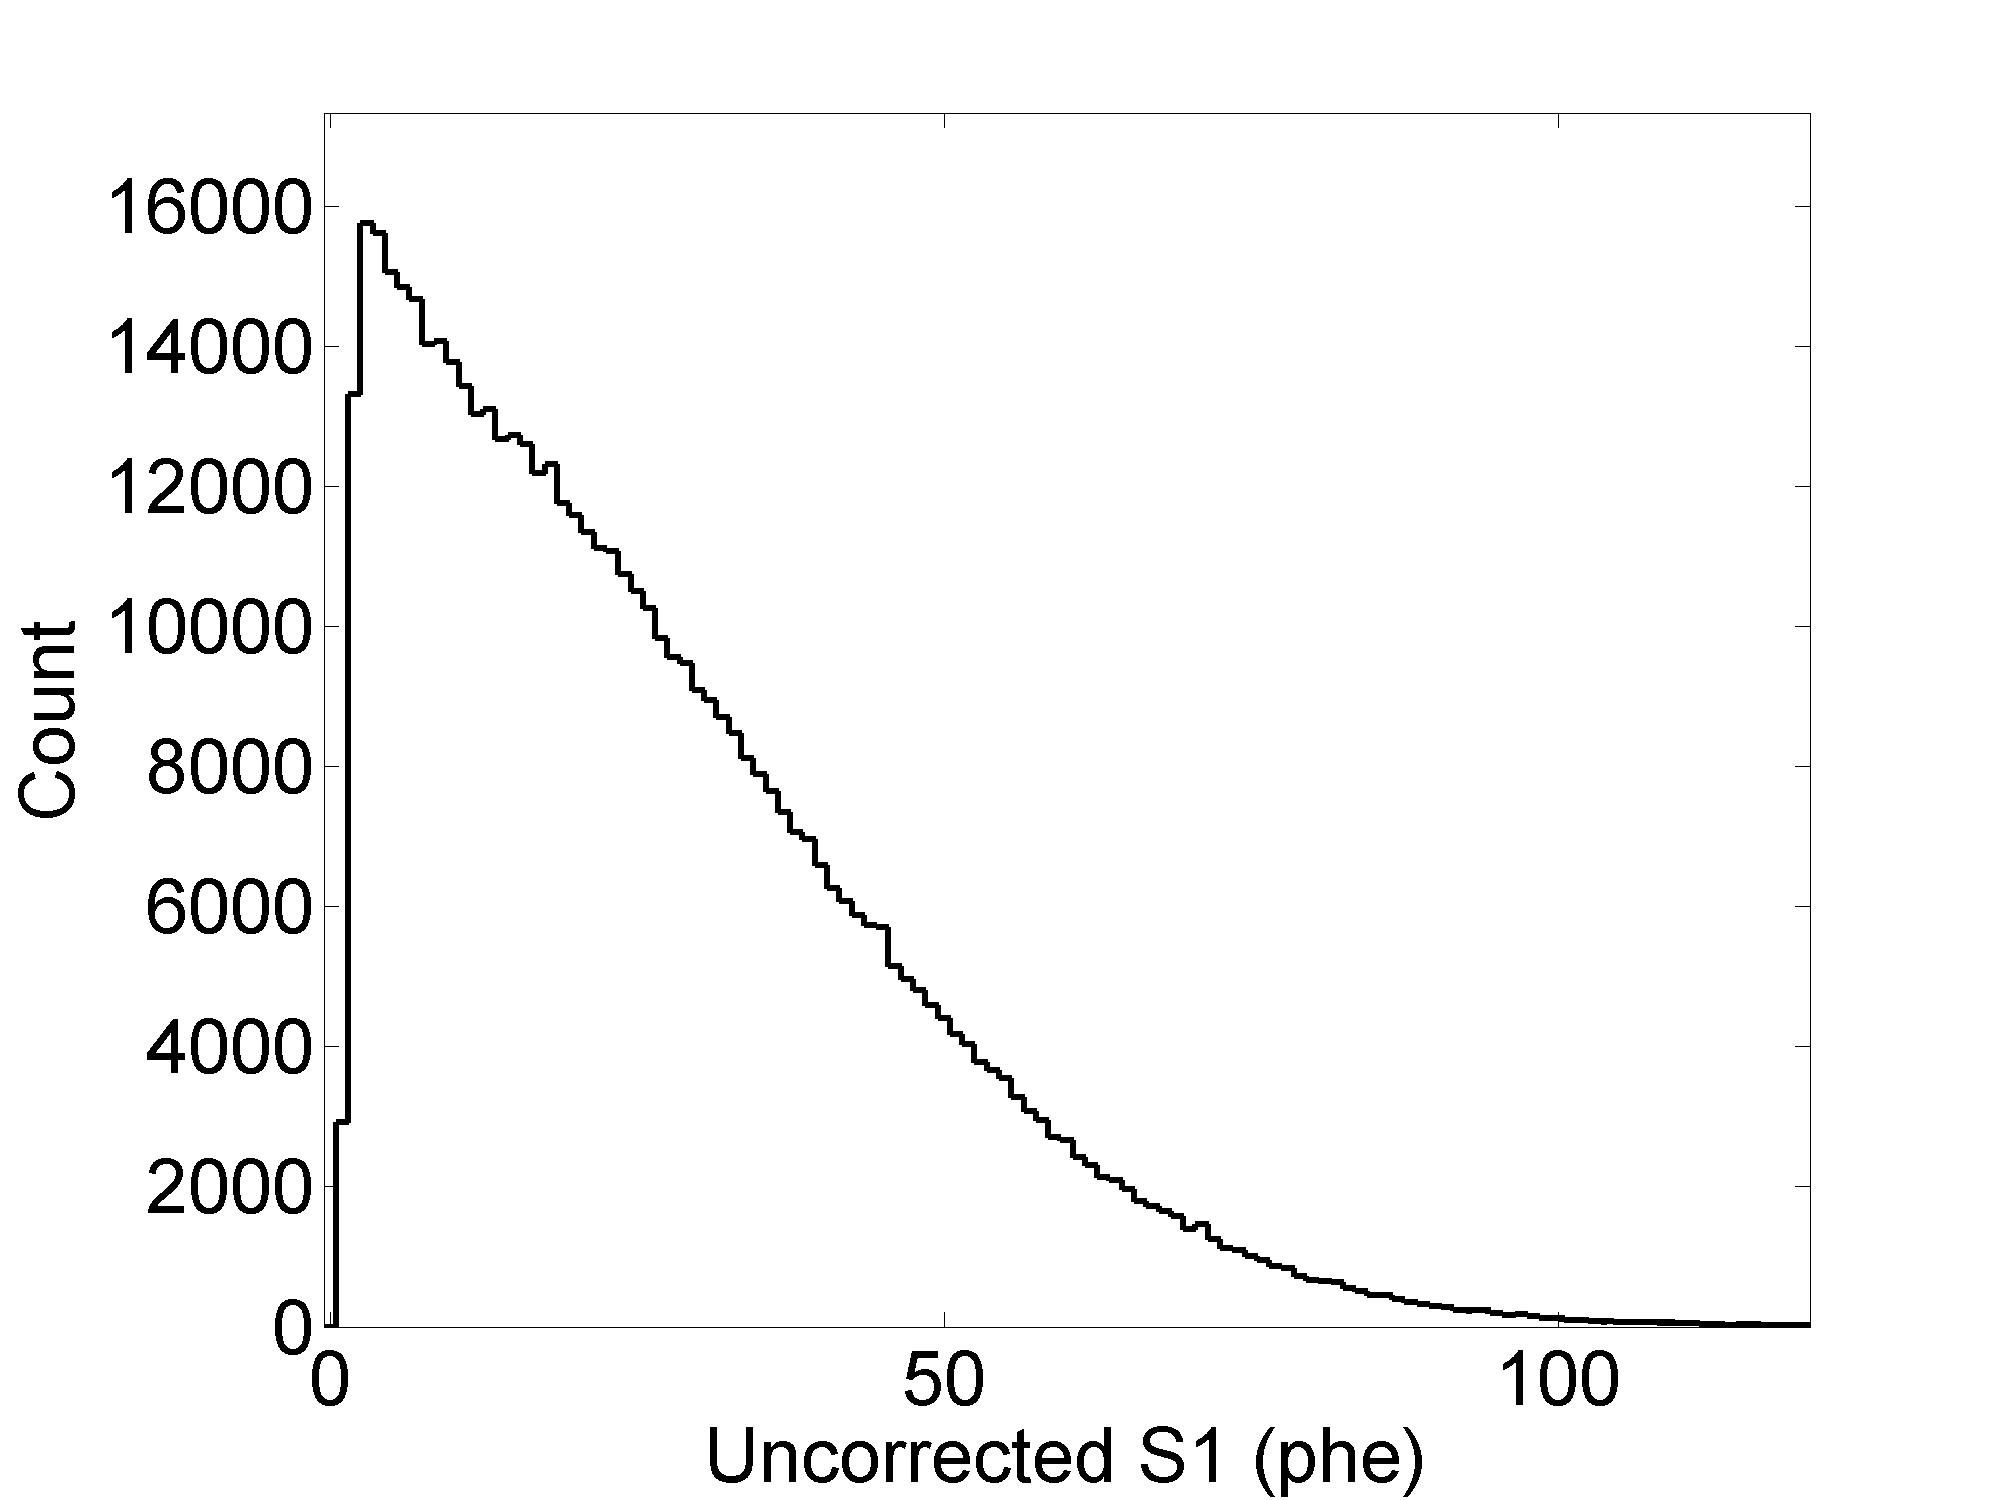
\includegraphics[scale=0.5]{Run04Corrections/CH3T_S1_Threshold.png}
\captionof{figure}{A histogram of uncorrected S1 data from the CH$_3$T calibration in September 2015.  The maximum of the distribution falls below threshold and can not be used for detector inefficiency corrections.}
\label{fig:S1thresholded}
\end{figure}

 
\subsubsection{Measuring Field Effects in $^{83m}$Kr Data} \label{section:FieldEffects}

After measuring the S2 detector inefficiency corrections in CH$_3$T data (equations~\ref{s2zcorr_eq} and~\ref{s2xycorr_eq}) we have all the tools we need to measure the field effects in the S2 pulse area of $^{83m}$Kr data.  We begin by applying the S2 detector inefficiency corrections to the raw,  uncorrected $^{83m}$Kr data (taken at the same time as the CH$_3$T data) by using equation \ref{E_eq}.  The removal of the detector inefficiency effects from the raw S2 data leave us with an S2$_E$ signal which has spatial pulse area variation from field effects alone.

The process for measuring the field effects in the inefficiency corrected $^{83m}$Kr S2$_E$ data is similar to the process of measuring the detector inefficiency effects in the field effect corrected CH$_3$T S2$_F$ data.  First, we measure the field induced Z dependence of the $^{83m}$Kr S2$_E$ pulse area by slicing the detector into drift time bins of 10 $\mu$s width.  A Gaussian distribution is fit to the S2$_E$ spectrum of each bin to determine the mean S2$_E$ pulse area versus Z. (Figure \ref{fig:GaussianPlot})  A cubic interpolation is used to determine the S2$_E$ Z dependence between each drift time bin, and a linear extrapolation based on the first and last 20\% of Gaussian fit data points is used to determine the S2$_E$ Z dependence above and below the span of the drift time bins (10-330 $\mu$s).  We define the strength of the field effect in the z direction as the ratio of the S2$_E$ pulse area as a function of Z to the S2$_E$ pulse area at the center of the detector $z_c$ (defined by taking the mean drift time value of all $^{83m}$Kr events above 4 $\mu$s drift time), S2$_E$(z)/S2$_E$(center). The strength of the field effect in September 2015 is consistent between a measurement with both PMT arrays and a measurement with the bottom-only PMT array. (Figure \ref{fig:KrZFieldEffect}) A field effect correction for the Z direction is defined by taking the inverse of the strength of the field effect, as described in the equation
\begin{equation}
\mbox{S}2_{\mbox{z-field-correction}} = \frac{S2_E(z=z_c)}{S2_E(z)}.
\end{equation} 


\begin{figure}[!h]
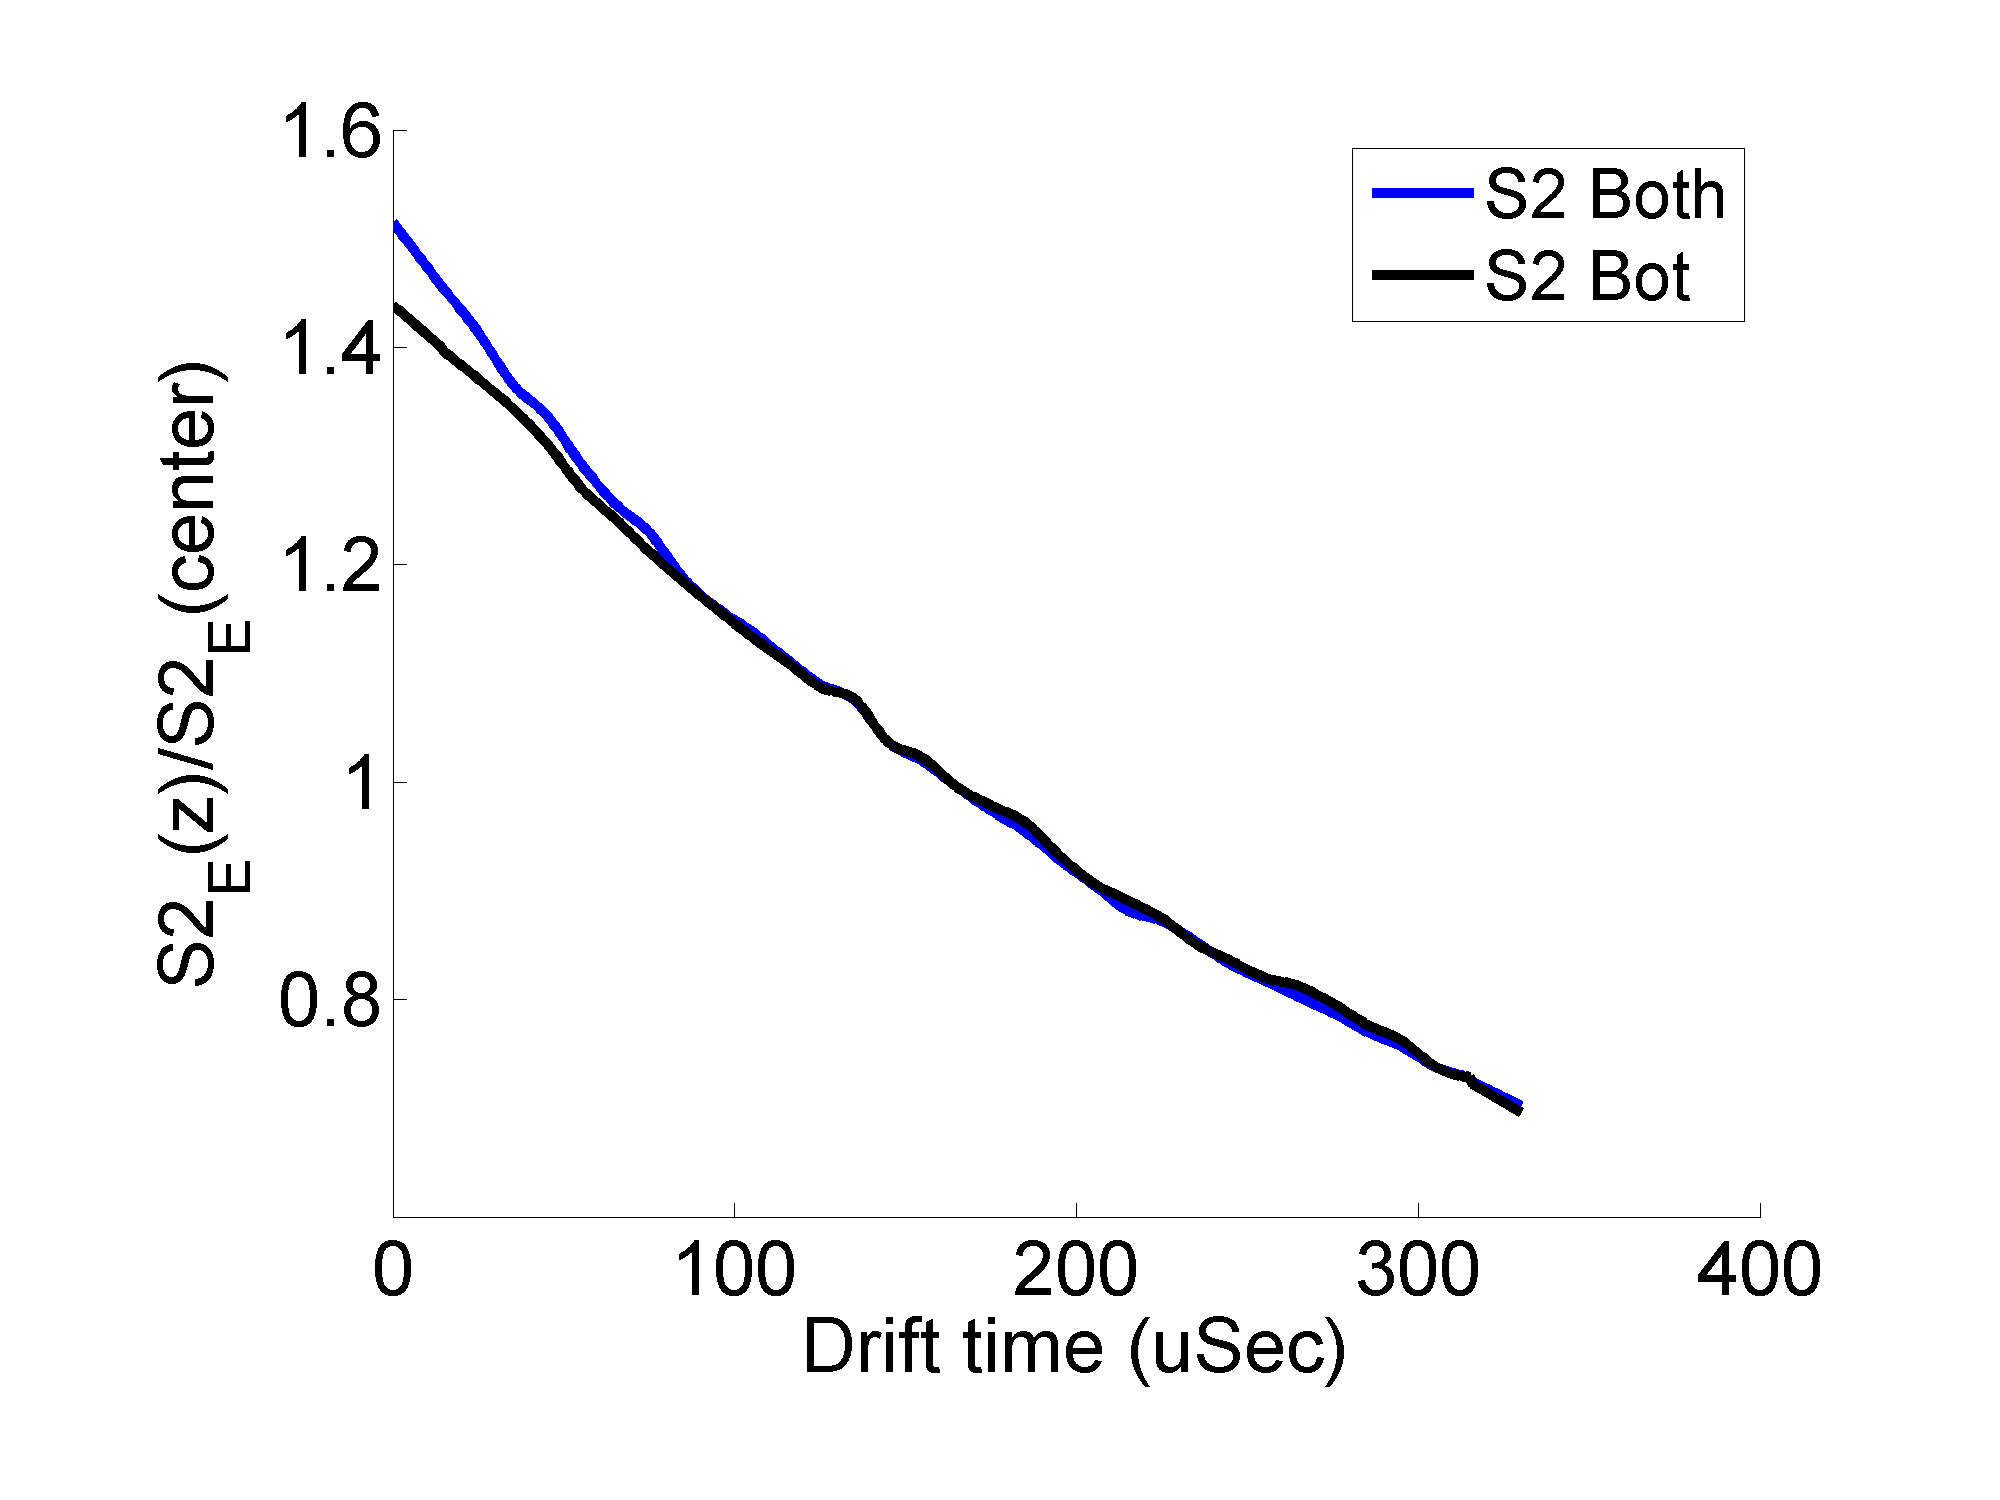
\includegraphics[scale=0.5]{Run04Corrections/FieldEffectZ_S2Only.png}
\captionof{figure}{The S2 field effect versus drift time relationship in $^{83m}$Kr data from September 2015.  The relationship was measured using both PMT arrays, and the bottom-only PMT array, and found to agree with both methods.}
 \label{fig:KrZFieldEffect}
\end{figure}

\begin{figure}[!h]
\centering
\subfloat{{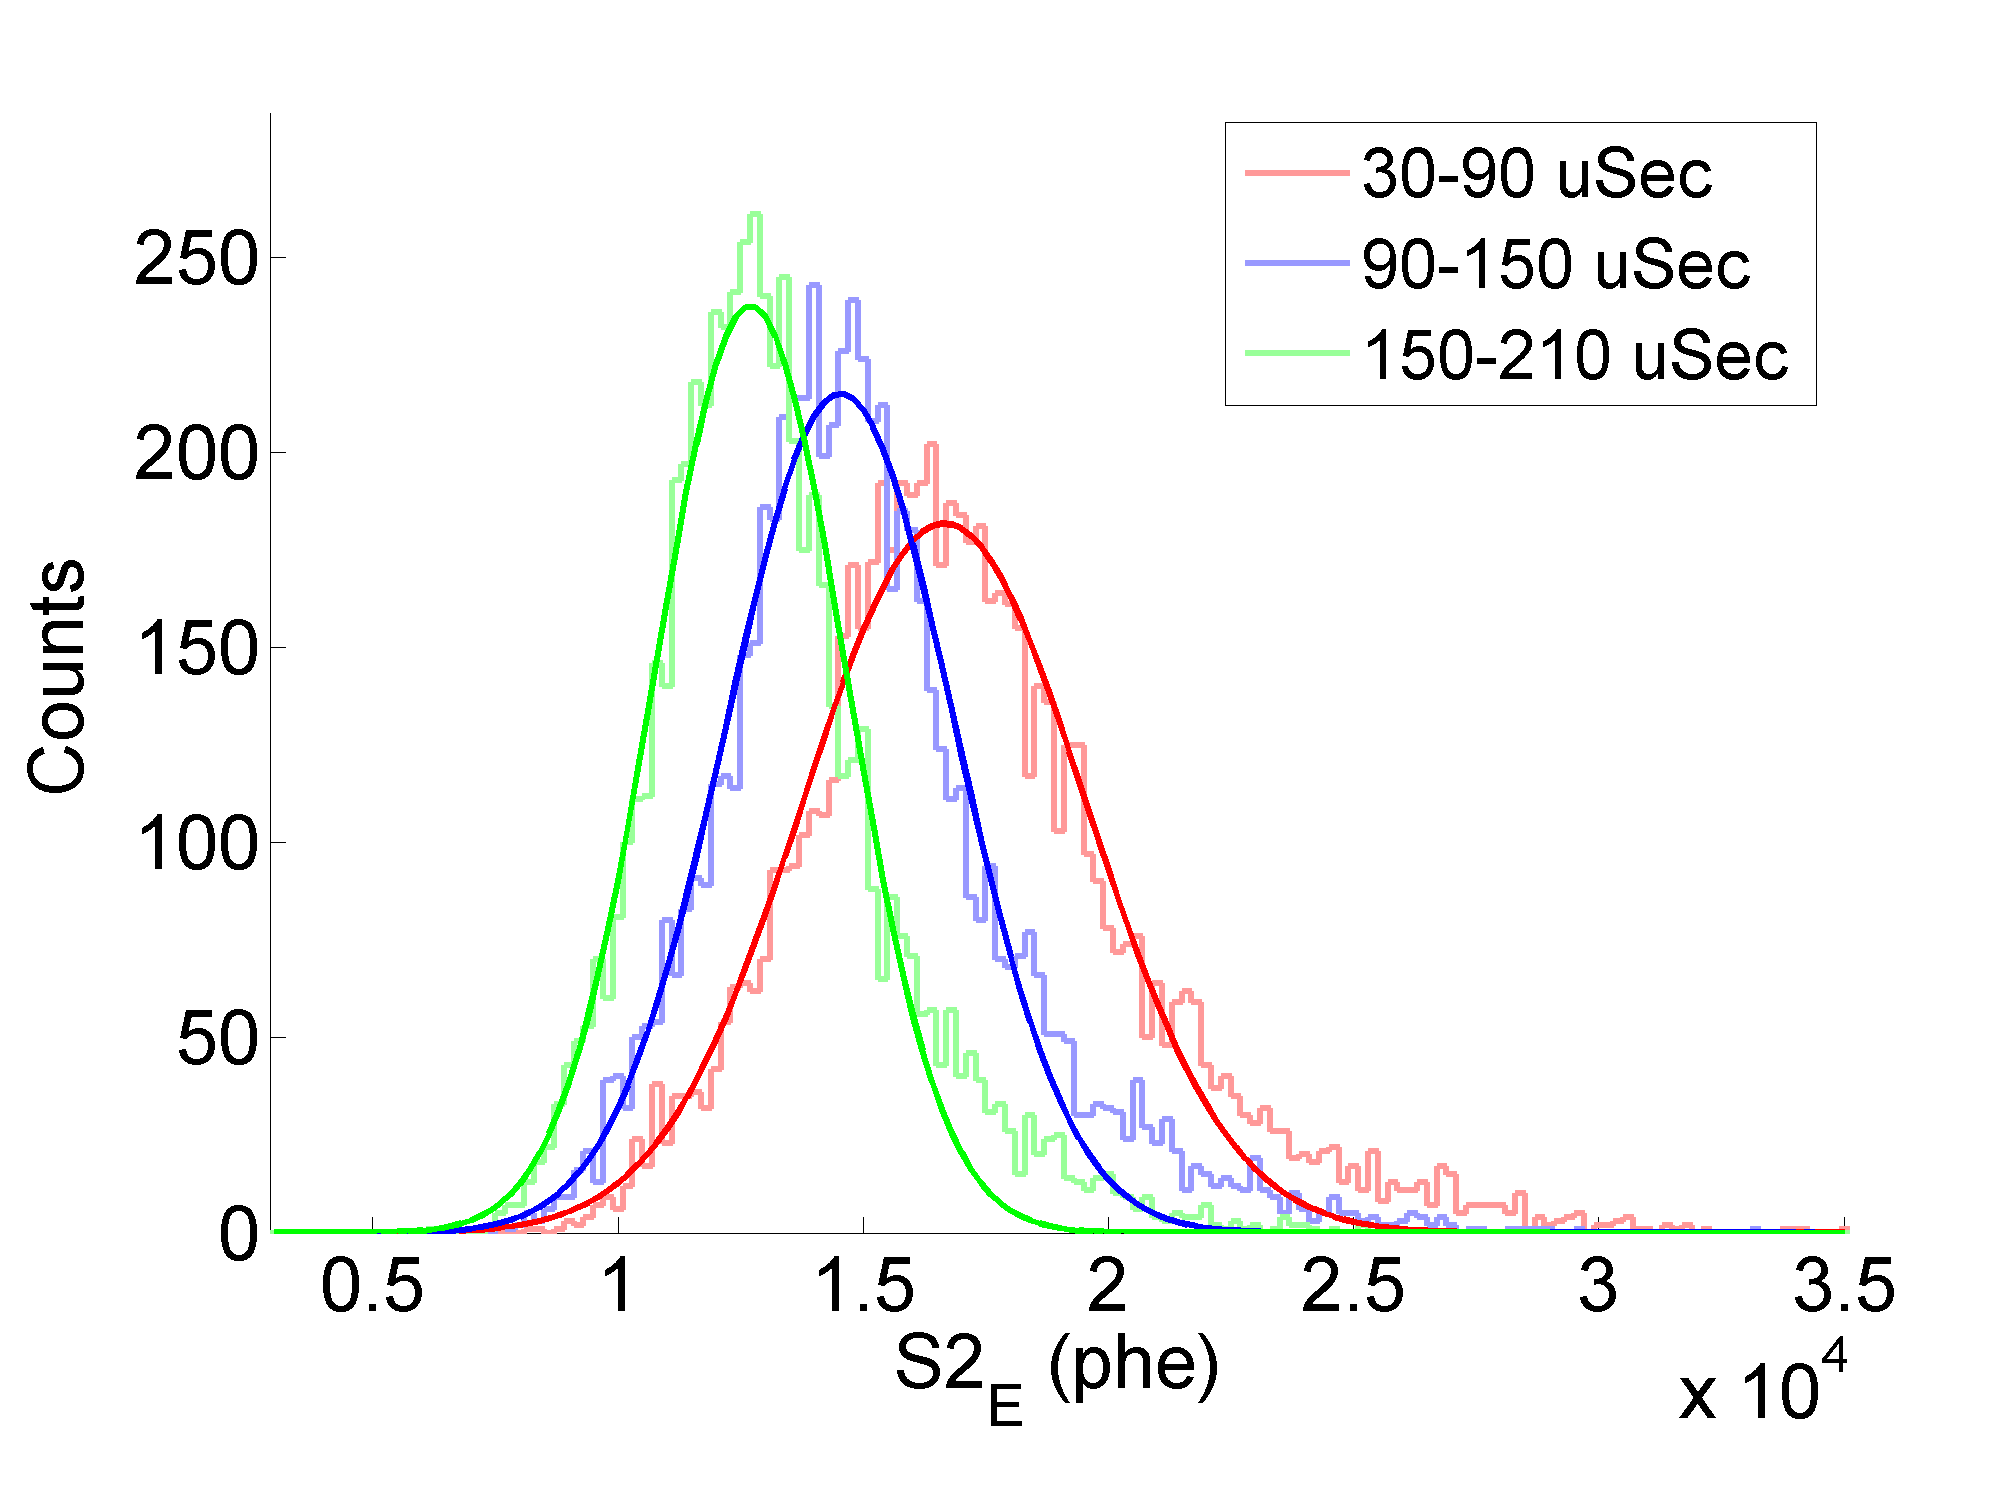
\includegraphics[width=6.5cm]{Run04Corrections/GaussianFits.png} }}
\qquad
\subfloat{{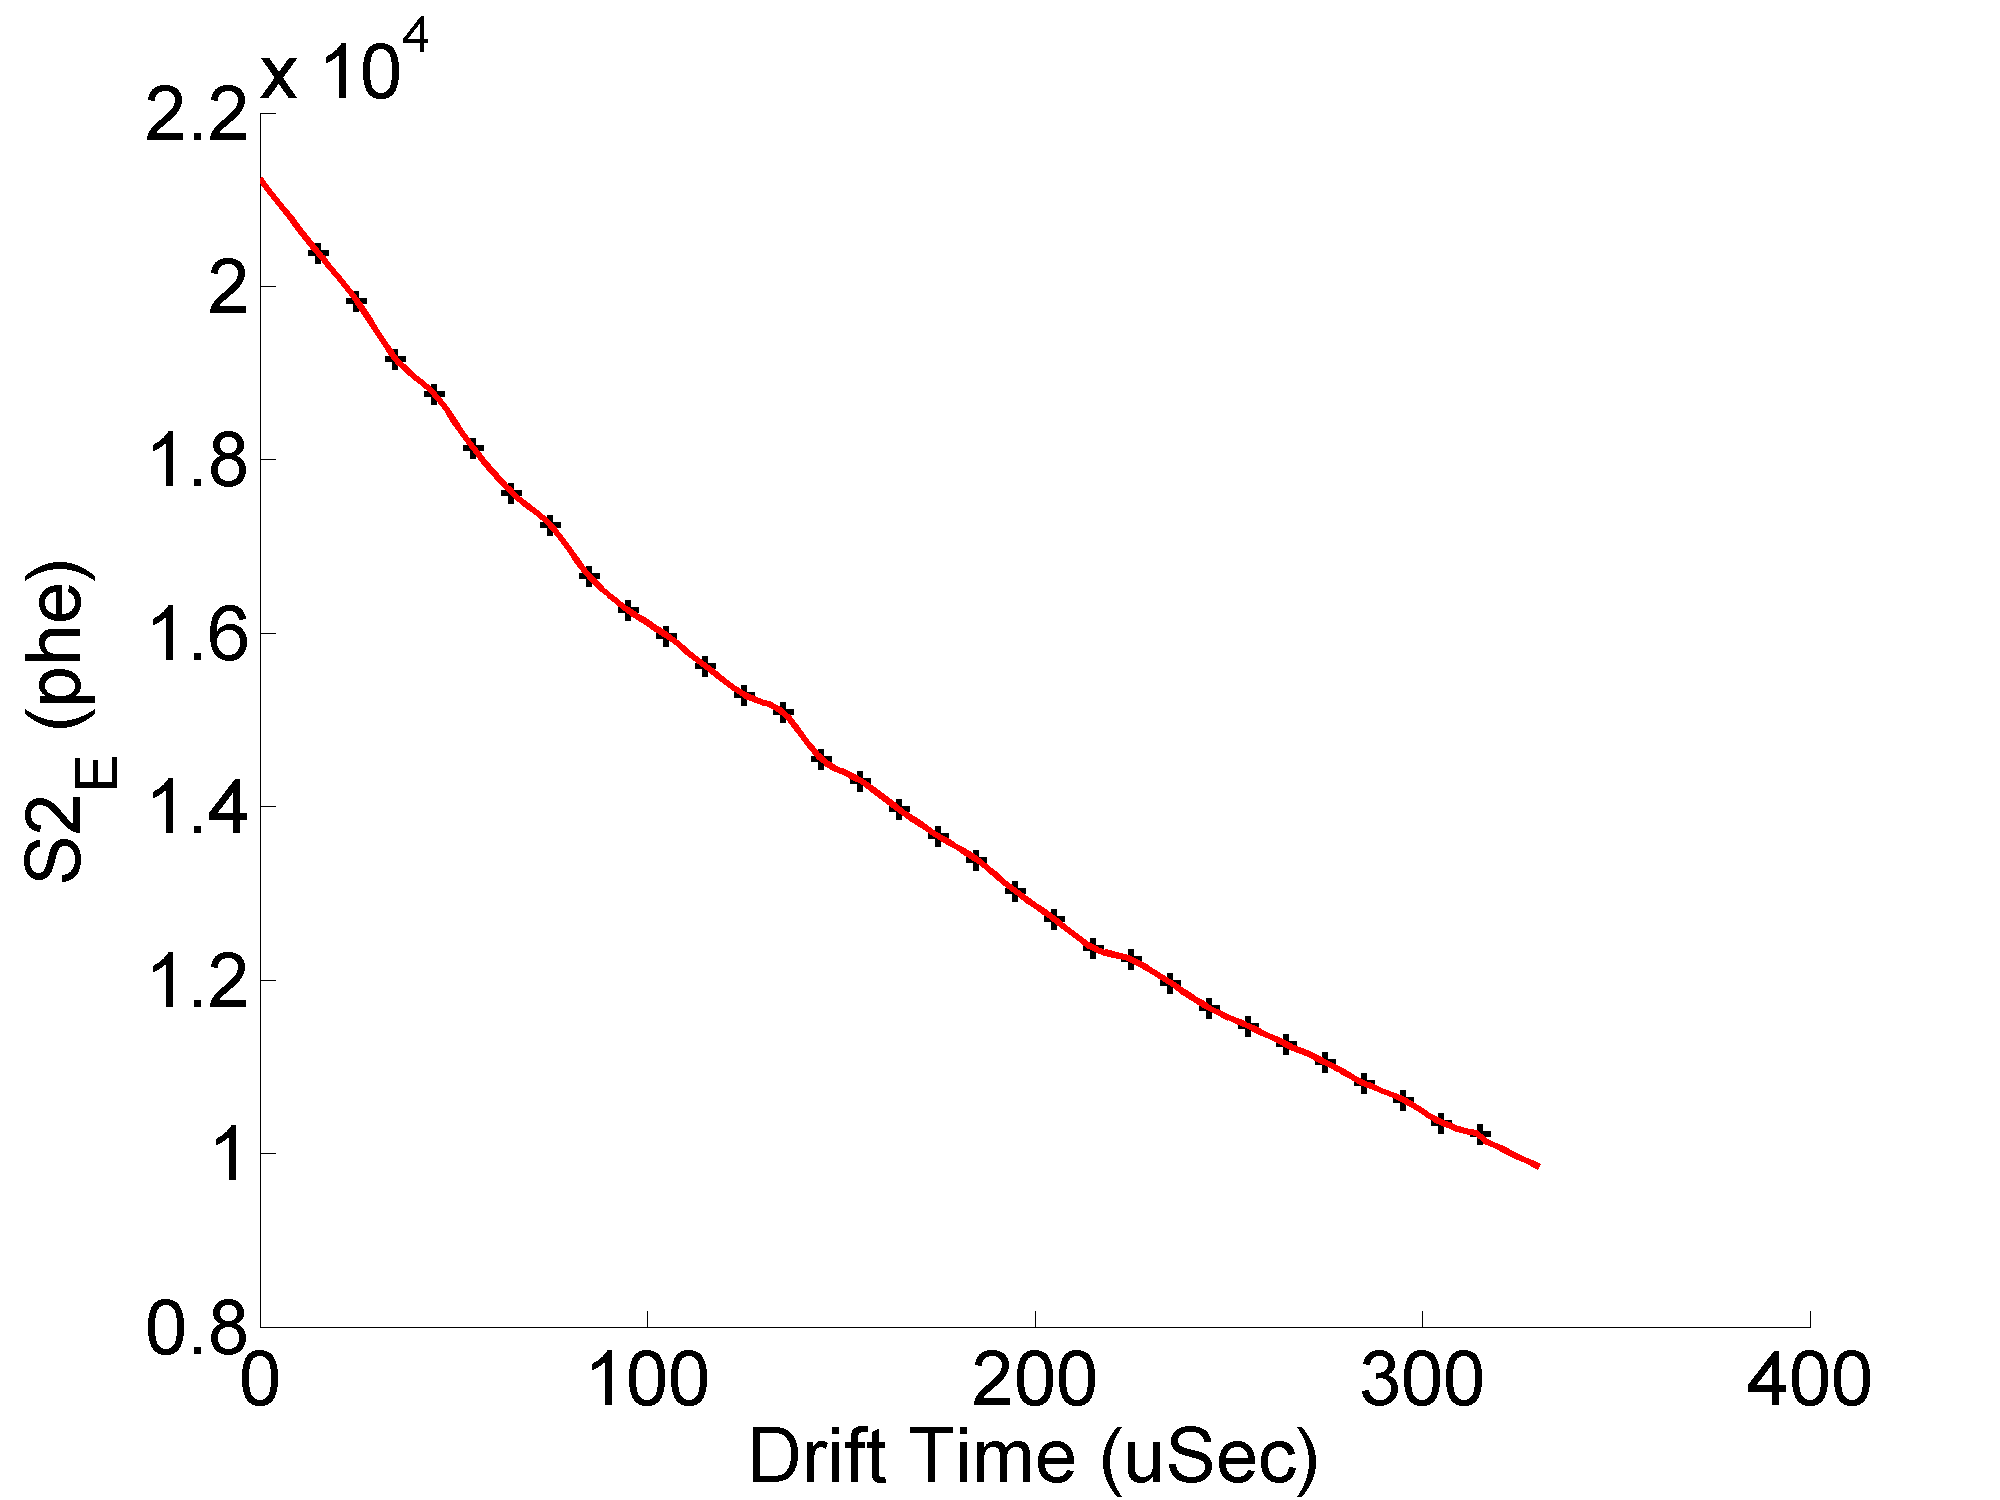
\includegraphics[width=6.5cm]{Run04Corrections/Kr_S2_ZDep.png} }}
\captionof{figure}{ (Left) Gaussian distribution fits to the $^{83m}$Kr S2$_E$ data that are used to determine the drift time dependence of the S2$_E$ pulse area. For illustrative purposes, a drift time bin width of 60 $\mu$s was chosen for this plot. (Right) The Z dependence of the $^{83m}$Kr S2$_E$ pulse area after detector inefficiency effects are removed.  Black points indicate the mean of Gaussian distribution fits for each drift time bin, and red line indicates the interpolation and extrapolation of that data.}
\label{fig:GaussianPlot}
\end{figure}


The XY dependence of the detector inefficiency corrected $^{83m}$Kr S2$_E$ signal is found by dividing the z field corrected (S2$_E \times \mbox{S}2_{\mbox{z-field-correction}}$) data into two dimensional XY bins with lengths of 2 cm on each side, and then fitting Gaussian distributions to the data of each bin.  The mean of the Gaussian distribution from each bin is used to construct an S2$_E$ XY dependence map, with a spline interpolation and extrapolation being used to determine the XY dependence between and outside of the bins. (Figure \ref{fig:KrXYDep}) A field effect correction for the XY direction is defined by taking the ratio of the z inefficiency corrected S2$_E$ pulse area at the center of the detector to the z inefficiency corrected S2$_E$ pulse area as a function of XY in cm, as shown below
\begin{equation}
\mbox{S}2_{\mbox{xy-field-correction}} = \frac{\mbox{S}2_{\mbox{z-field-correction}}\times S2_E(x_c,y_c,z)}{\mbox{S}2_{\mbox{z-field-correction}}\times S2_E(xyz)}.
\end{equation} 
where $x_c$ and $y_c$ are the x and y center of the detector in uncorrected coordinates determined by taking the average position of the $^{83m}$Kr events in each direction.

\begin{figure}[!h]
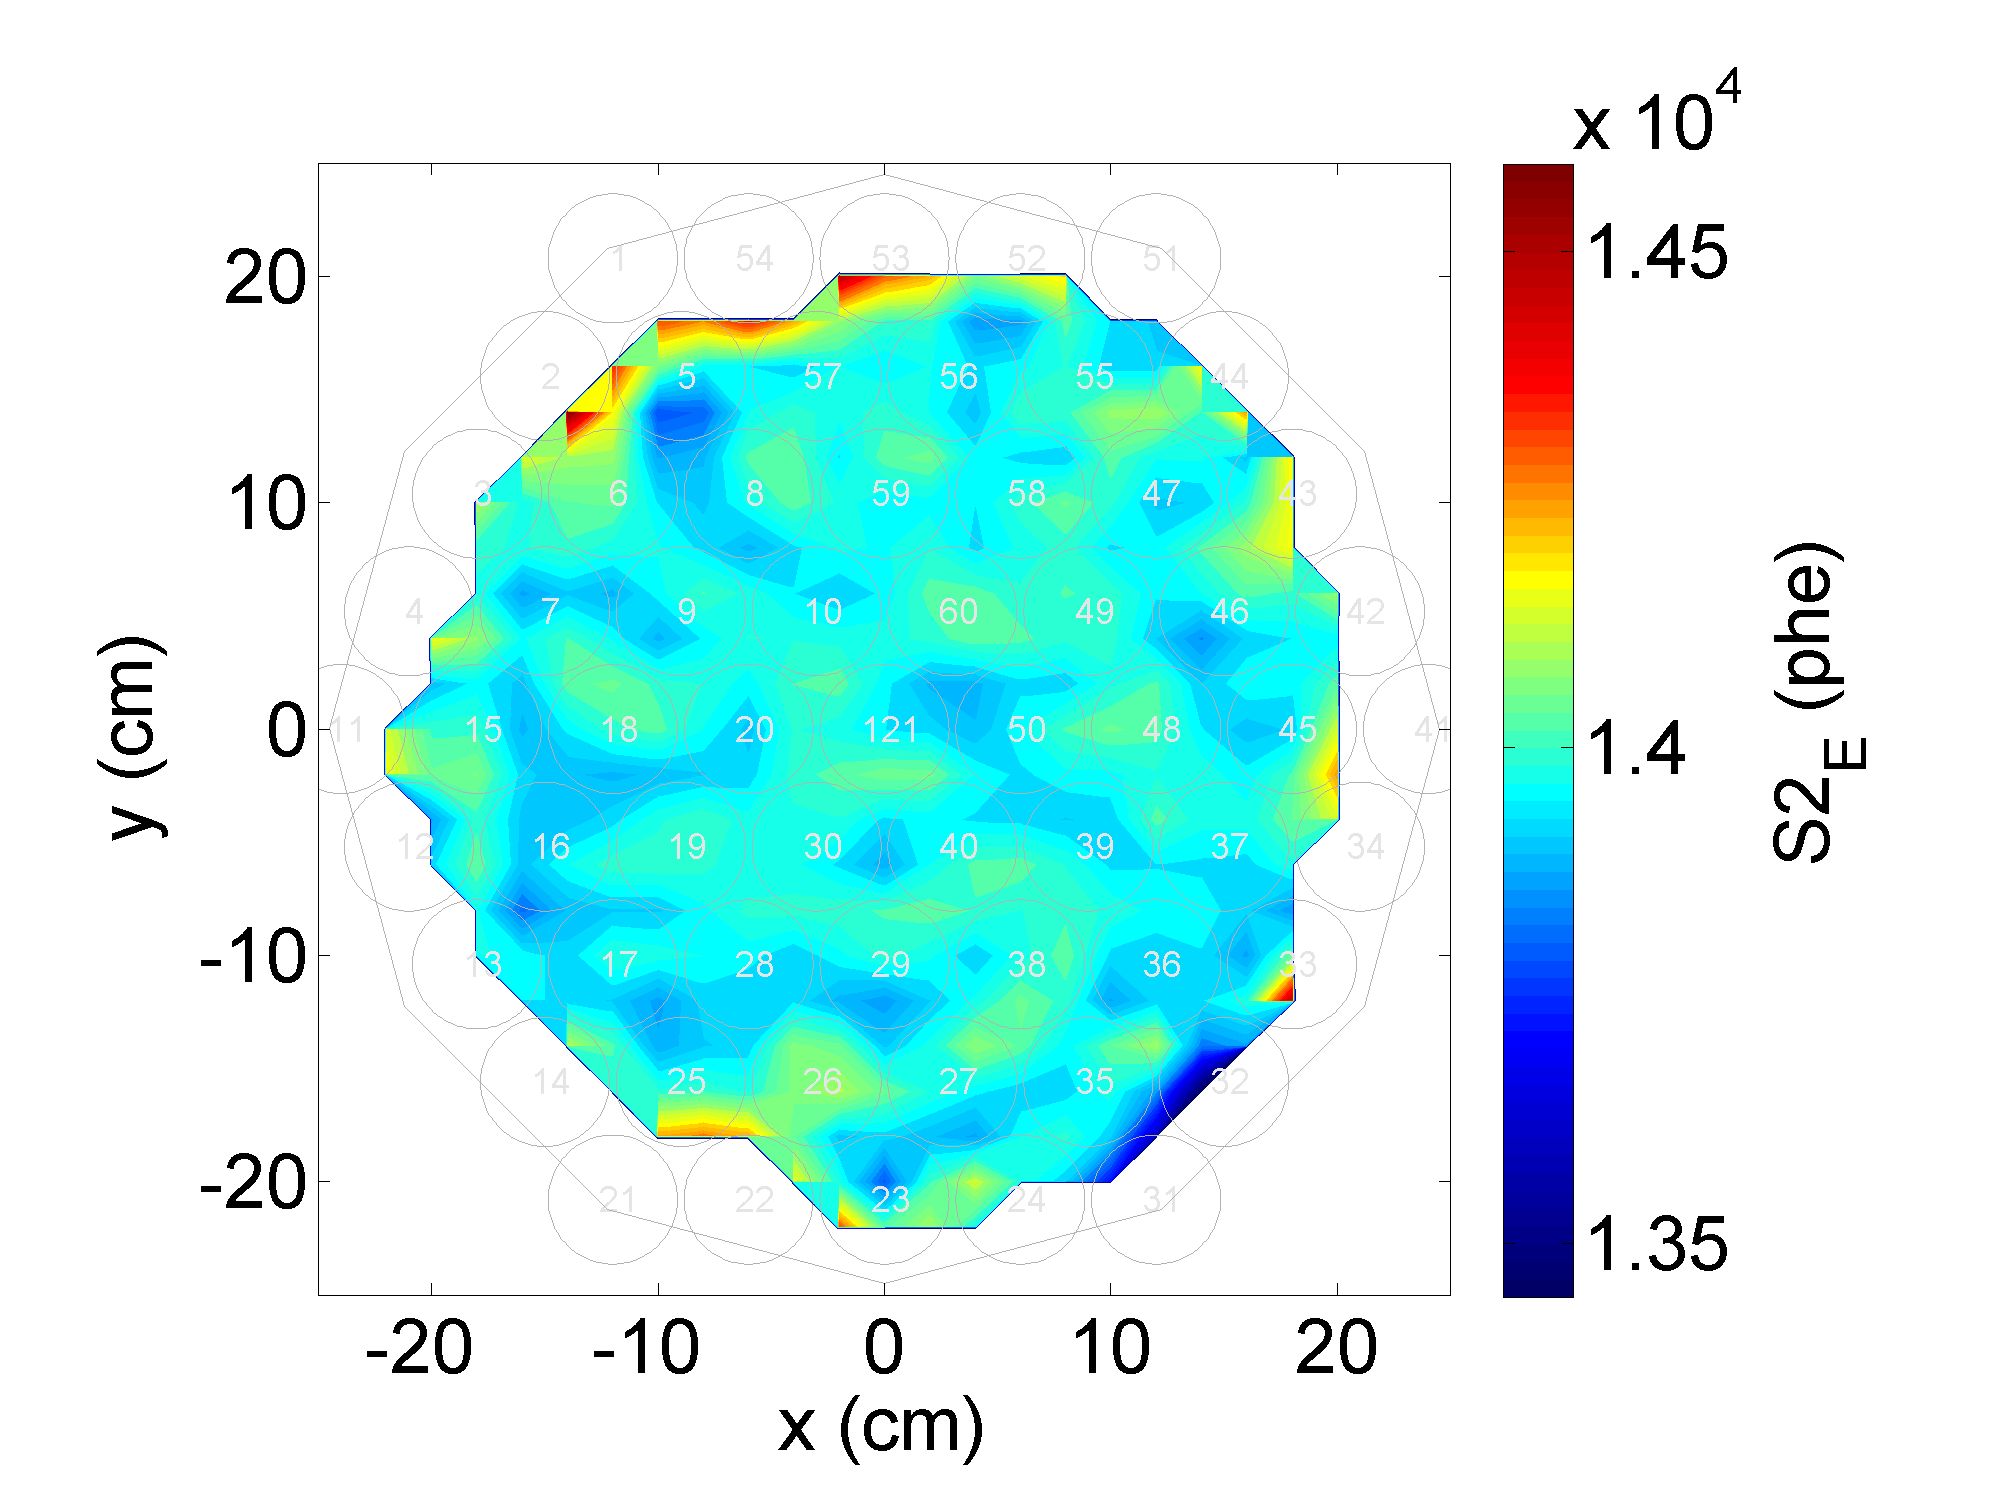
\includegraphics[scale=0.45]{Run04Corrections/Kr_S2_XYDep.png}
\captionof{figure}{Two dimensional map of the XY dependence in $^{83m}$Kr S2$_E$ data determine by fitting a Gaussian distribution to XY bins of the data and tracking the mean of each fit.}
 \label{fig:KrXYDep}
\end{figure}

We also take a separate, three dimensional approach to mapping the field effect in the $^{83m}$Kr S2$_E$ data. In this approach the detector is divided into three dimensional voxels, with X and Y width of 3.5 cm and Z width of 30 $\mu$s.  As in the one dimensional (Z) plus two dimensional (XY) case, a three dimensional map of the field induced S2$_E$ pulse area variation is produced by fitting a Gaussian distribution to the $^{83m}$Kr S2$_E$ data in each voxel.  A spline interpolation is used to determine the S2$_E$(xyz)/S2$_E$(center) ratio between the three dimensional voxels, and the S2$_E$(xyz)/S2$_E$(center) Z dependence map is used to extrapolate outside of the range of the voxels.  The three dimensional map is used in the final analysis, with the 1D plus 2D approach used for extrapolation purposes only.

\subsubsection{Measuring the S1a and S1b Pulse Areas in $^{83m}$Kr data} \label{section:S1aS1b1}

Now that we have measured the field effect in $^{83m}$Kr S2 data from the $^{83m}$Kr S2$_E$ data at one point in time, we need to develop a method to track the field effect in $^{83m}$Kr S2 data at all points in time.  To accomplish this we use the uncorrected S1 pules area from the 32.1 keV and 9.4 keV decays within $^{83m}$Kr events, referred to as S1a and S1b respectively.  As discussed in section \ref{section:NEST}, as the electric field increases the amount of recombination decreases, leading to a smaller S1 signal.  The S1a decay is more sensitive to this effect due to its higher energy, leading to a stronger field effect in the S1a data than in the S1b data.   Therefore, an inverse relationship exists between the strength of the field and the S1a/S1b ratio.  

A MATLAB module is used to measure the size and location of the S1a and S1b krypton decays~\cite{S1aS1bModuleNote}. It selects $^{83m}$Kr event with an S2 pulse area pulse area between 2000 to 60000 phe as measured by the bottom PMT array.  The module identifies S1 candidates that have pulse area above 10 phe (as measured by both PMT arrays), such that each $^{83m}$Kr event is defined to have exactly one candidate S2 and at least one candidate S1.  After the event selection is complete, a region of interest (ROI) beginning at the first candidate S1 and ending at the start of the S2 (or after 150 samples) is defined. The ROI is then used to select sumpod (phd per sample) data from the evt files within the ROI.  This data is then fit to a double exponential function which returns the pulse area and maximum fractional area of the S1a and S1b peaks, as well as the time separation between them. (Figure \ref{fig:Sumpod}) The MATLAB module does not produce reasonable fit values for events in which the S1a and S1b decays are separated by less than 13 samples, so a cut requiring the timing to be greater than this is used to clean up the output of the module.  (Figure~\ref{fig:S1aS1btiming})

Note that the correlation seen in Figure~\ref{fig:S1aS1btiming} is a result of both detector inefficiencies and field effects.  Detector inefficiencies induce a one-to-one correlation between S1a and S1b.  On the other hand, field effects cause S1a and S1b to vary by differing amounts, introduce less of a correlation.

\begin{figure}[!h]
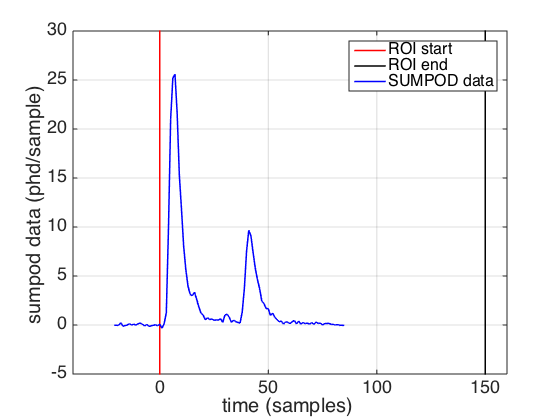
\includegraphics[scale=0.6]{Run04Corrections/s1a_s1b_sumpod.png}
\captionof{figure}{Sumpod versus time for a $^{83m}$Kr in which a distinct S1a and S1b peak have been observed. In this case, the fit finds an S1a area of 174 phe, an S1b area of 64.5 phe, and a separation in time of 35 samples.}
 \label{fig:Sumpod}
\end{figure}

\newpage

\begin{figure} [!h]
\centering
\subfloat{{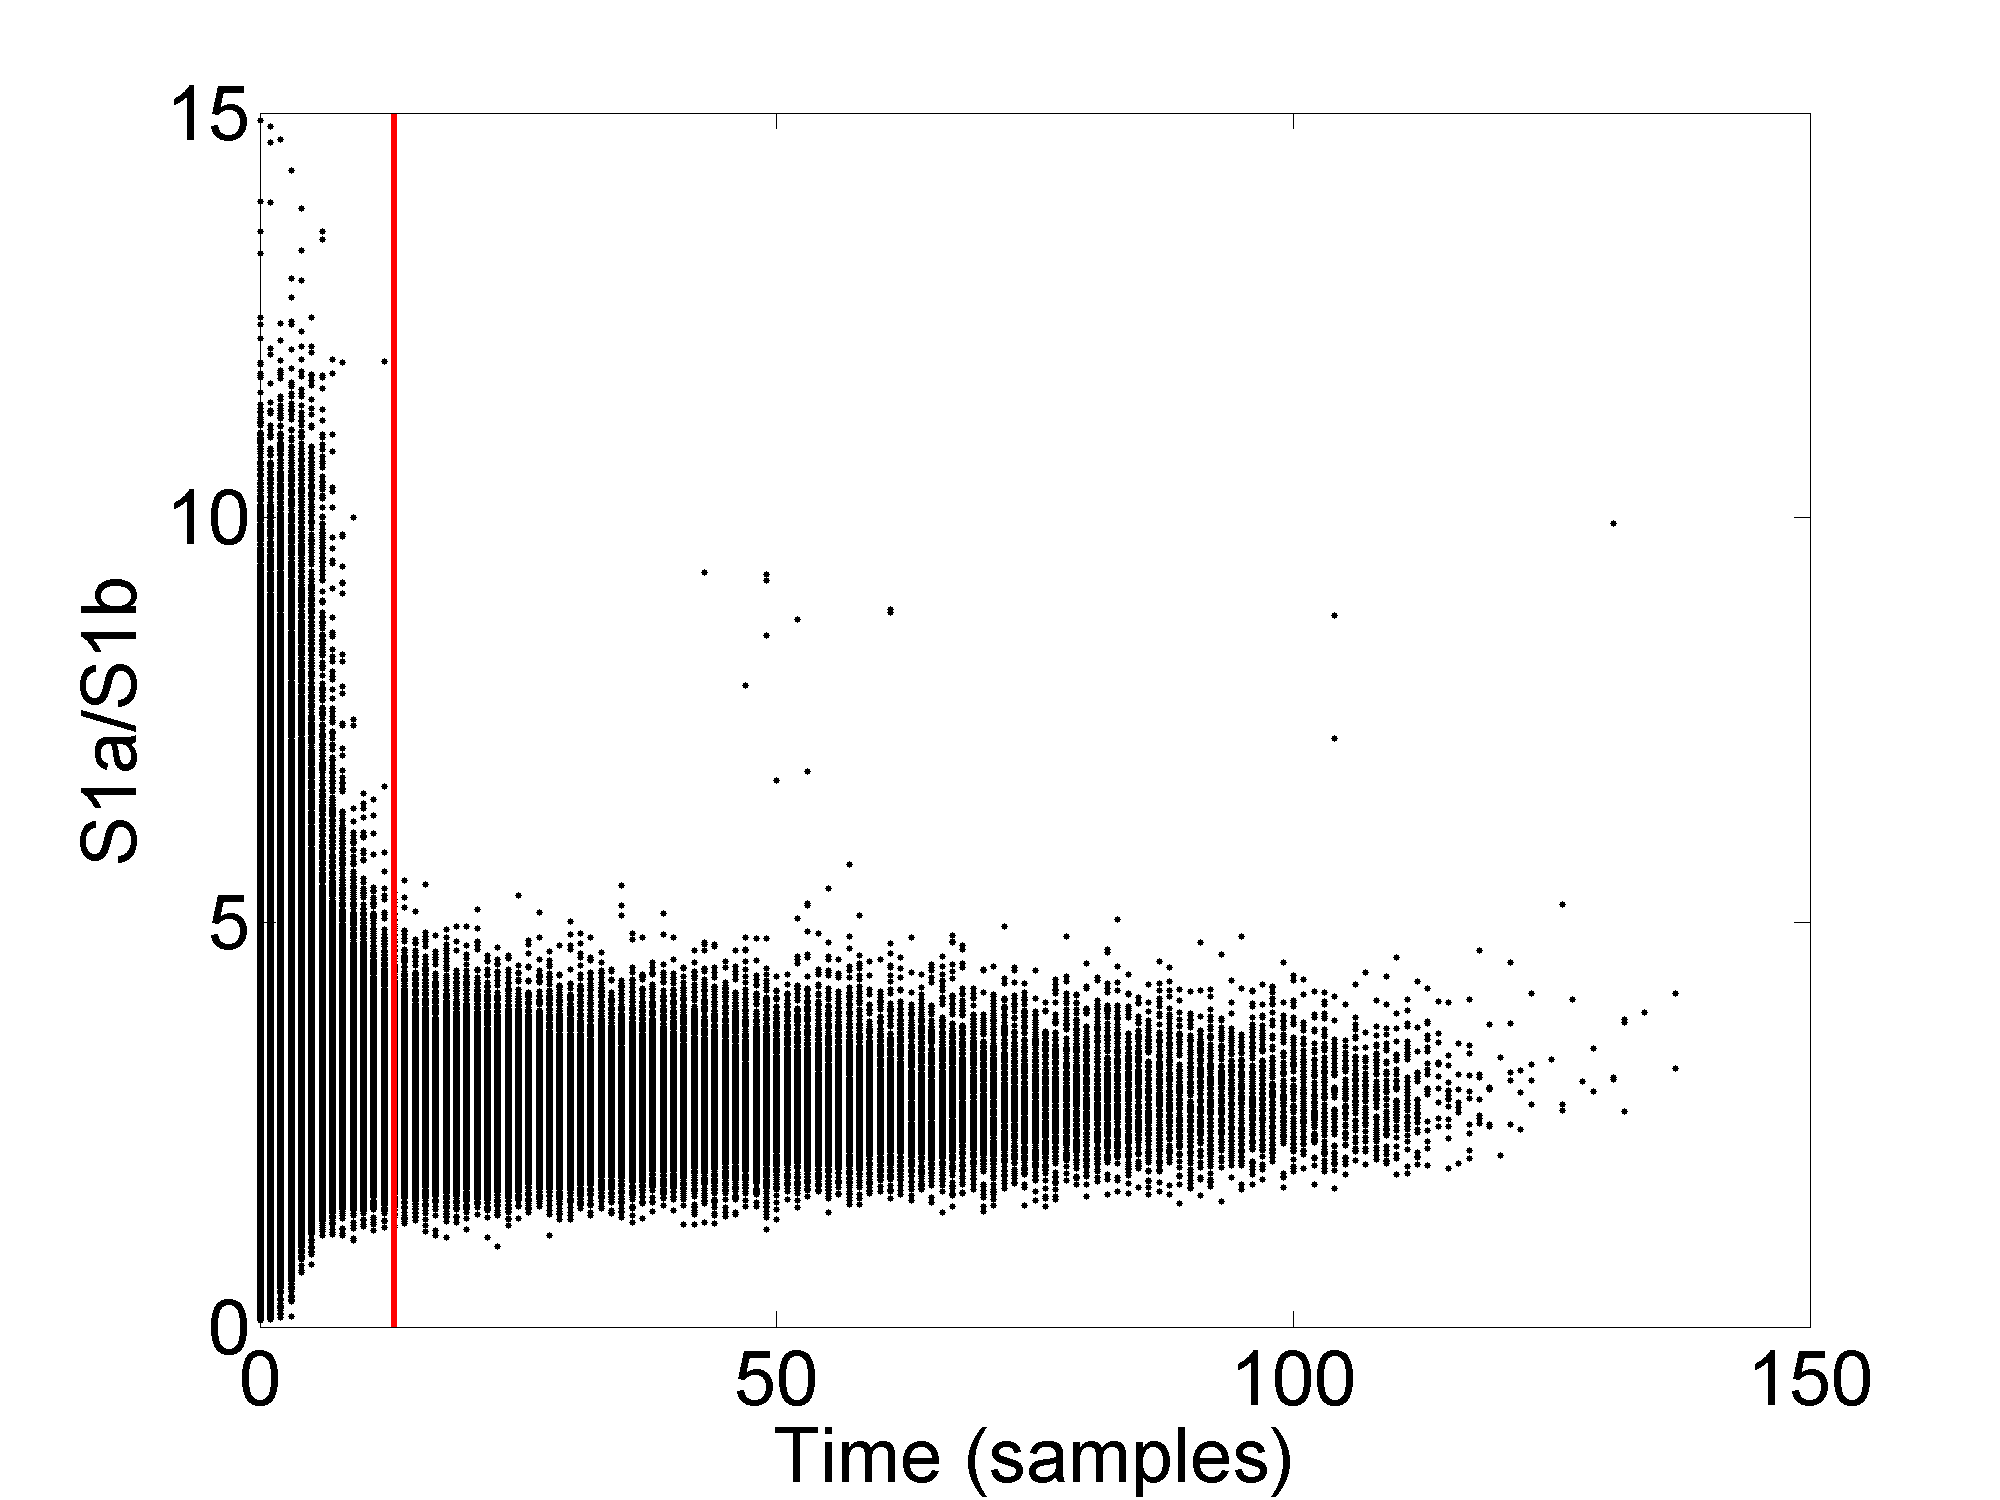
\includegraphics[width=11cm]{Run04Corrections/S1aS1bCut_Timing.png} }}
\qquad
\subfloat{{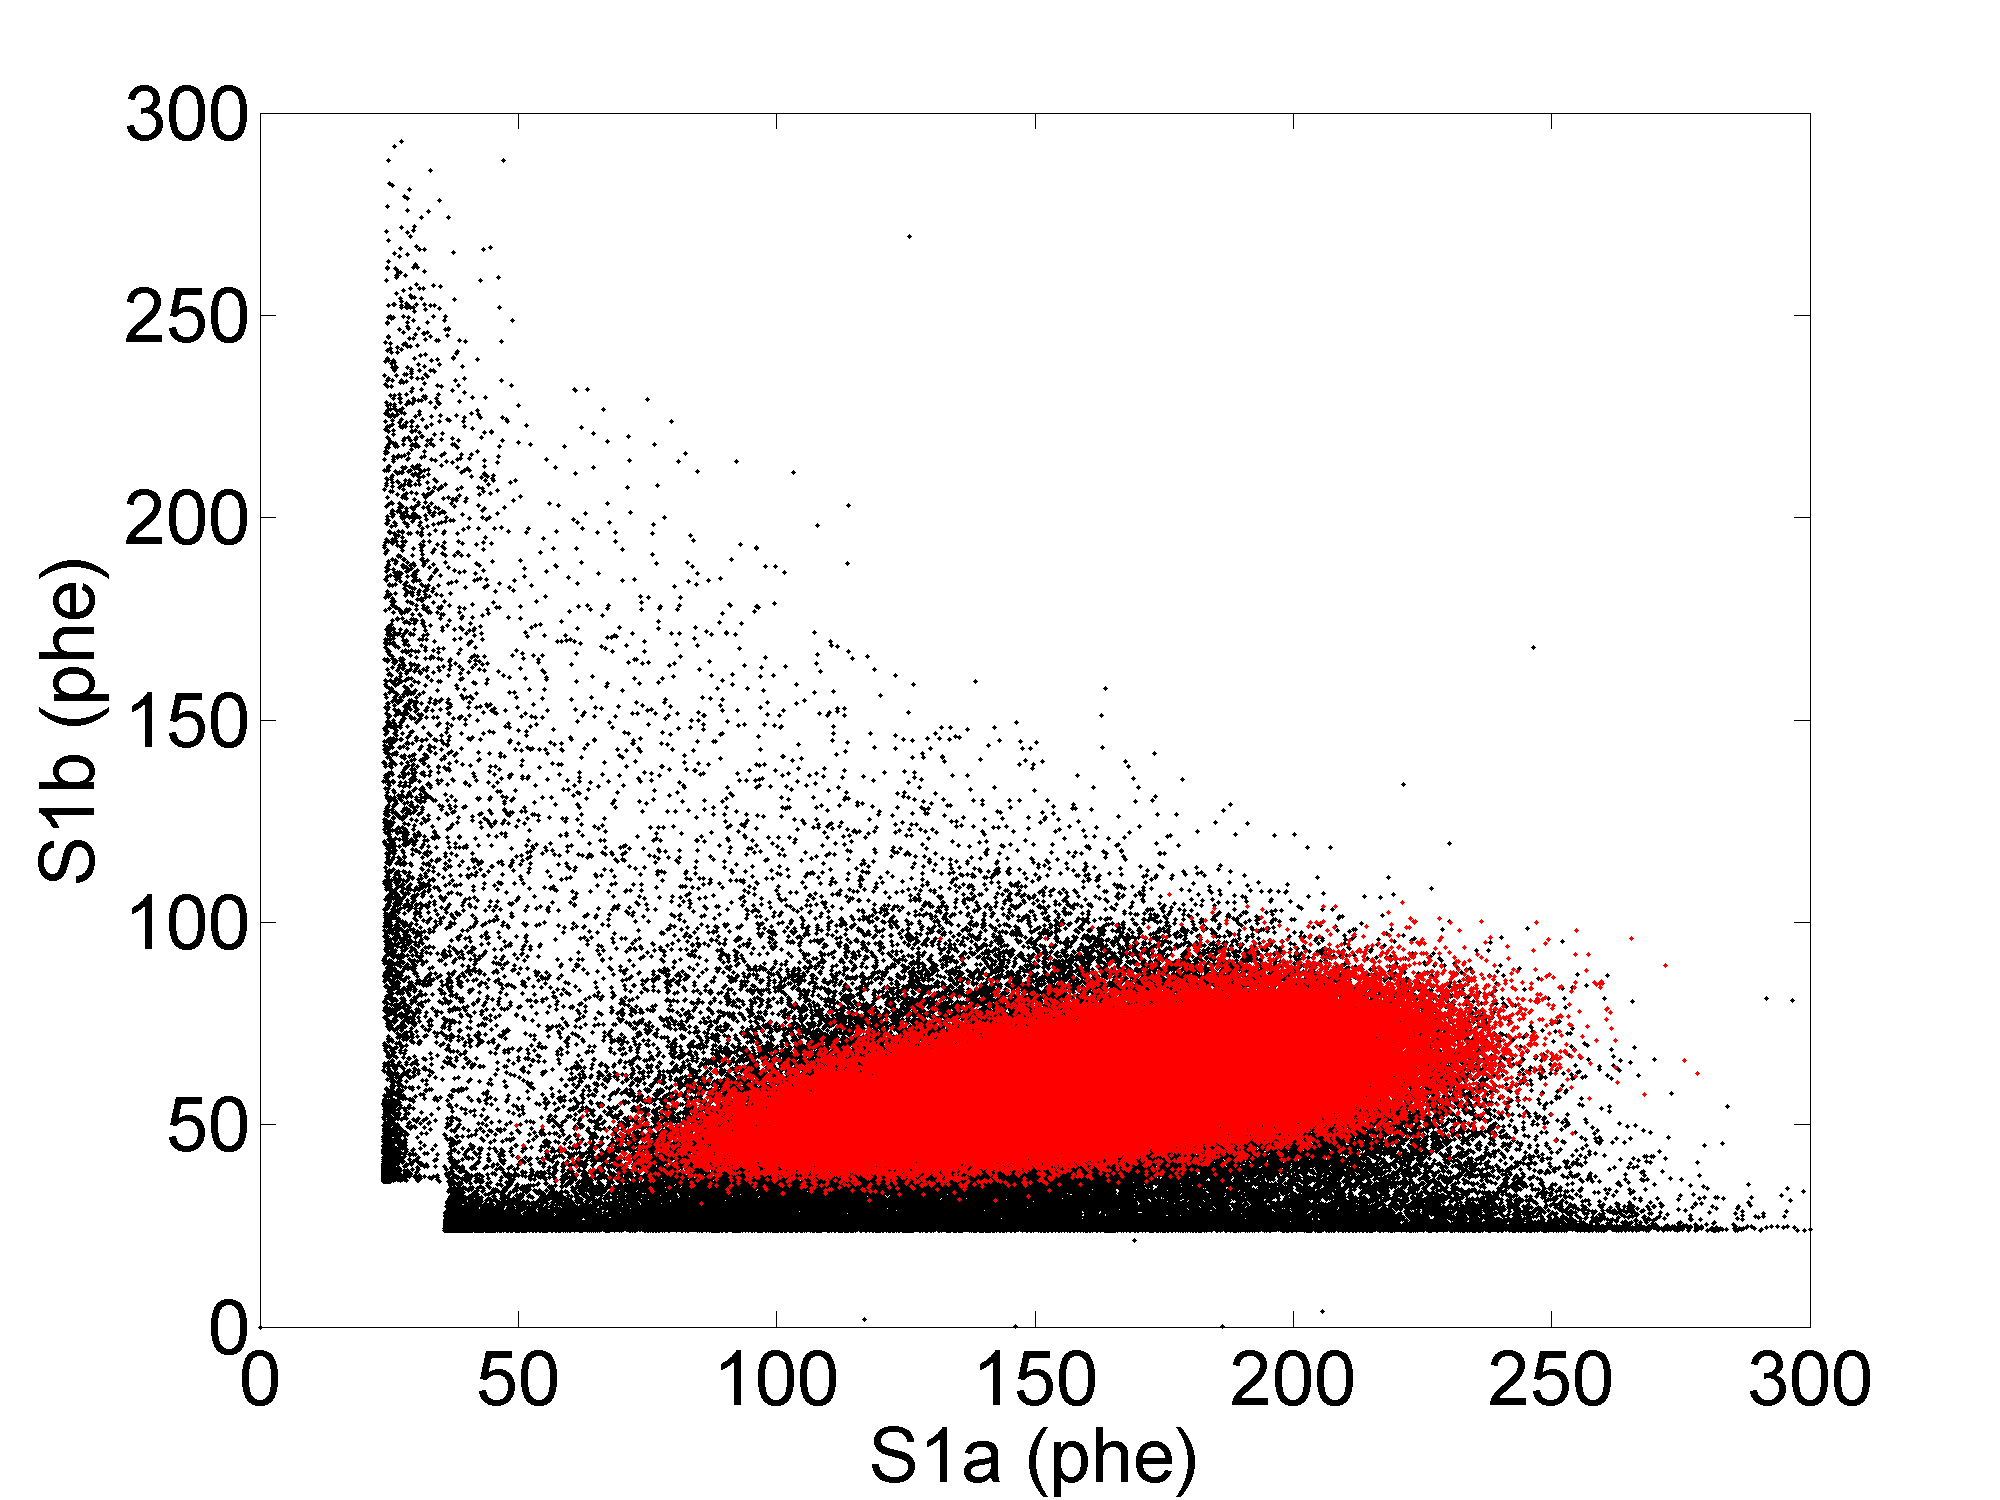
\includegraphics[width=11cm]{Run04Corrections/S1aS1bCut.png} }}
\captionof{figure}{ (Top) The output of the S1a/S1b fitting module as a function of time separation between the two decays.  The red line indicates the 13 sample minimum separation between the S1a and S1b events required by our cut in this analysis. (Bottom) A scatter plot of all S1a and S1b pulse areas measured by the fitting module (black) compared to the S1a and S1b pulse areas that are left after our selection cut. (red) Data from lux10\_20150929T1905\_cp17540.}
\label{fig:S1aS1btiming}
\end{figure}


\subsubsection{Relating the S1a/S1b Ratio to S2 Field Effects} \label{section:S1aS1b2}

To relate the S1a/S1b ratio to the S2 field effects measured in section \ref{section:FieldEffects} we begin by measuring the spatial dependence of the S1a/S1b ratio.  We first divide the detector into drift time bins of 
3 $\mu$s width.   A Gaussian distribution is fit to the S1a and S1b spectrum of each bin to determine the mean pulse areas versus Z. (Figure \ref{fig:S1aGaussianPlot})  A second order polynomial is fit to the ratio of the Gaussian means versus Z and is used to determine the S1a/S1b ratio at any drift time in the detector.  


\begin{figure} [!h]
\centering
\subfloat{{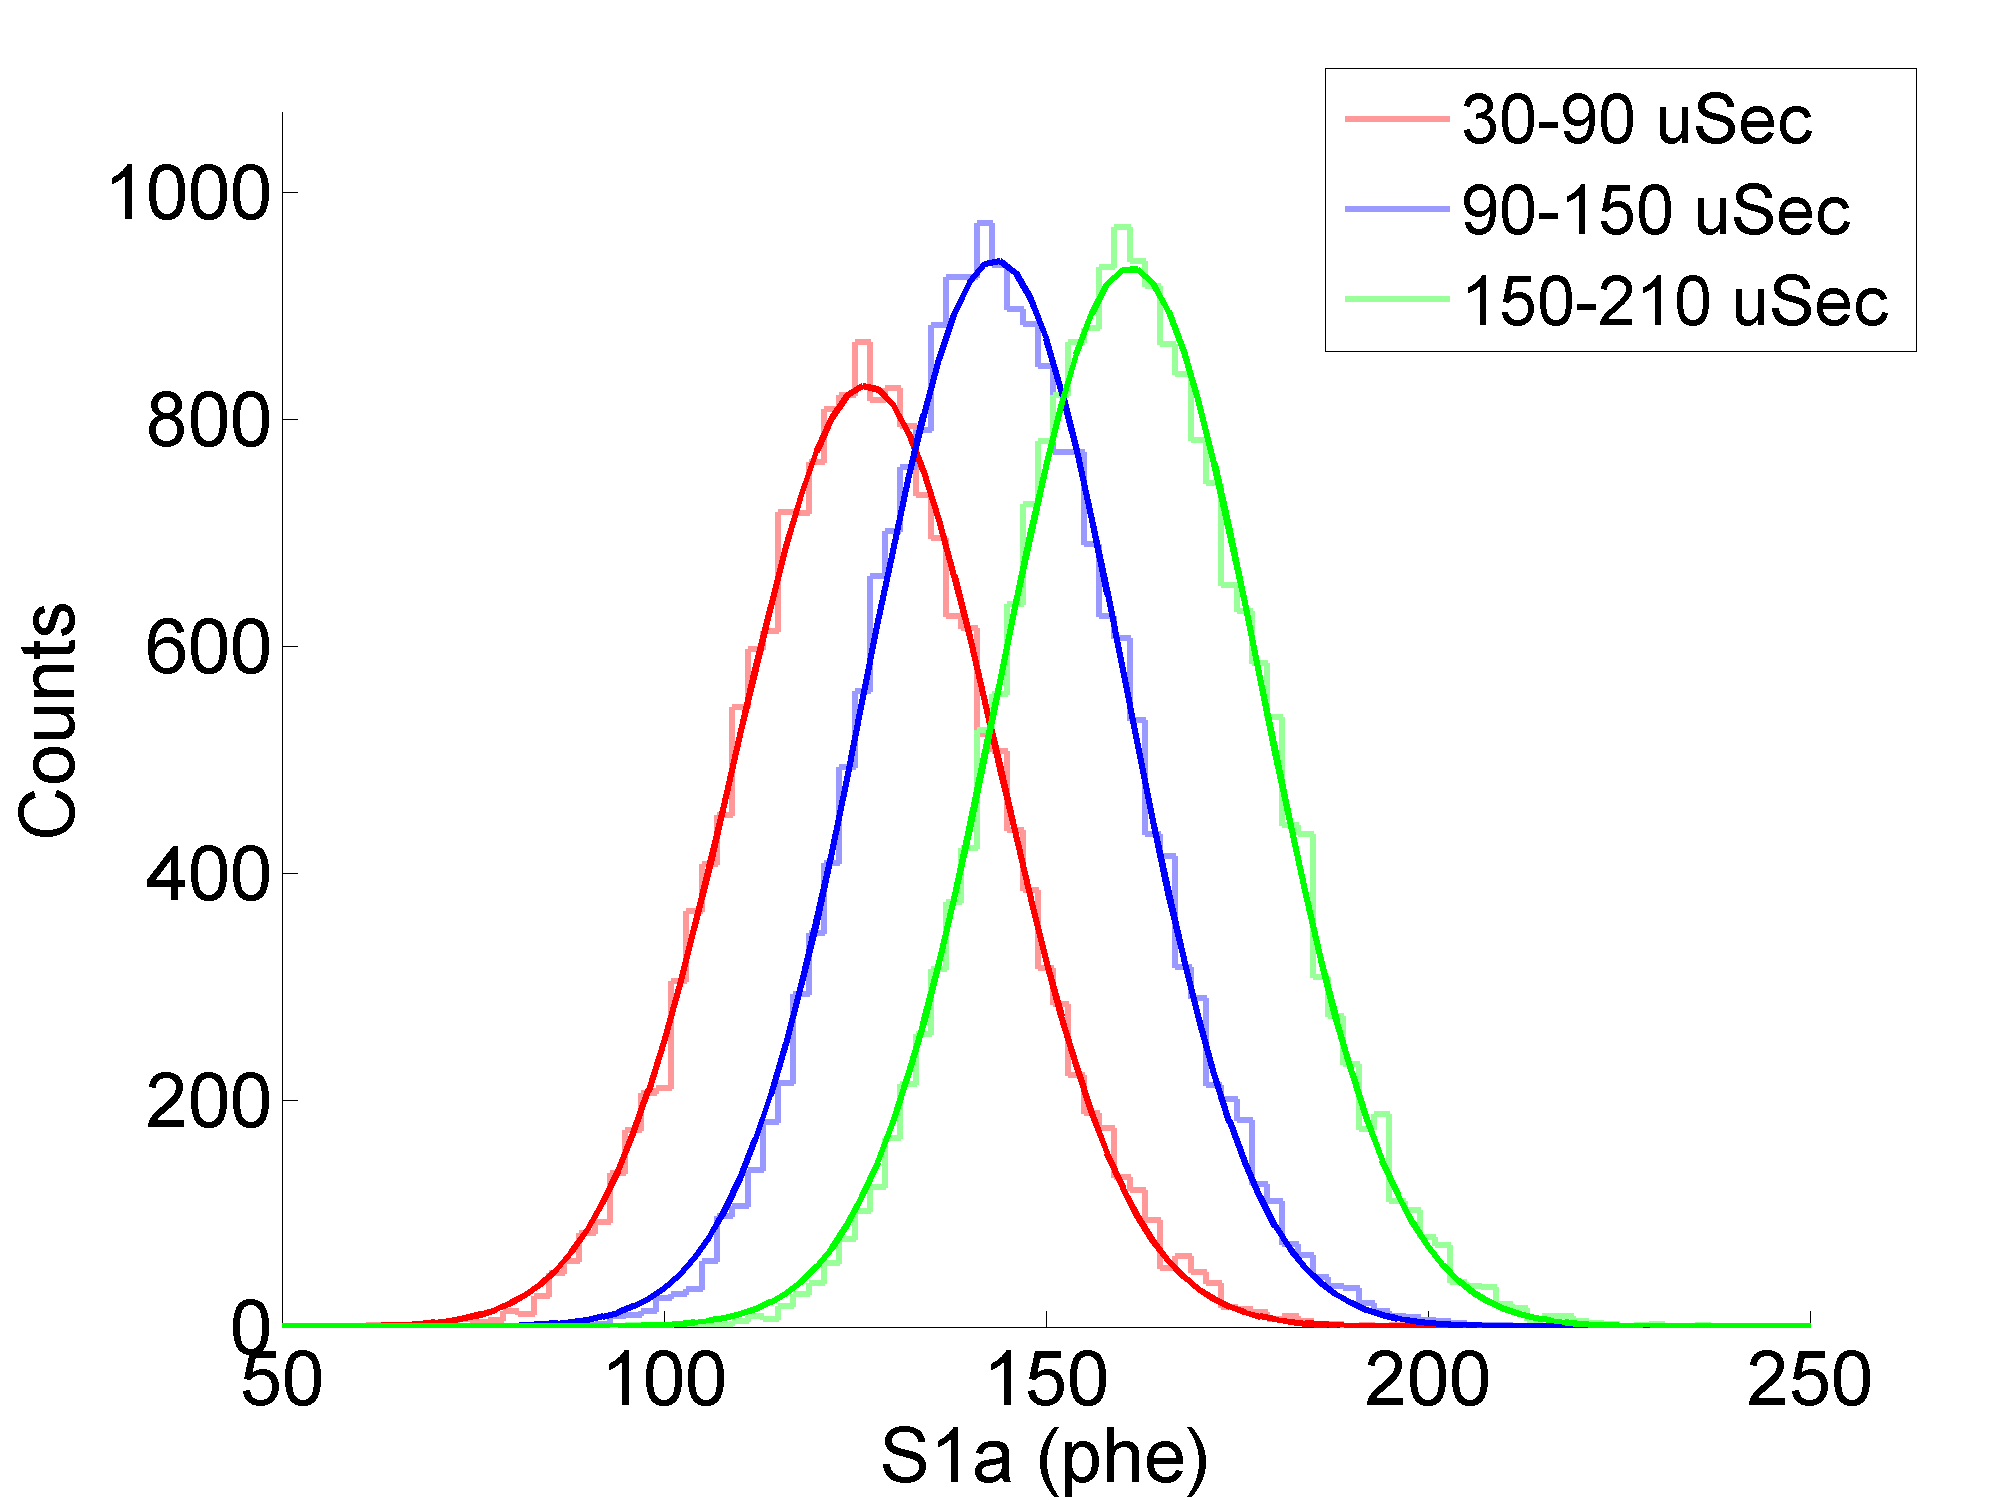
\includegraphics[width=6.5cm]{Run04Corrections/S1aGaussianFits.png} }}
\qquad
\subfloat{{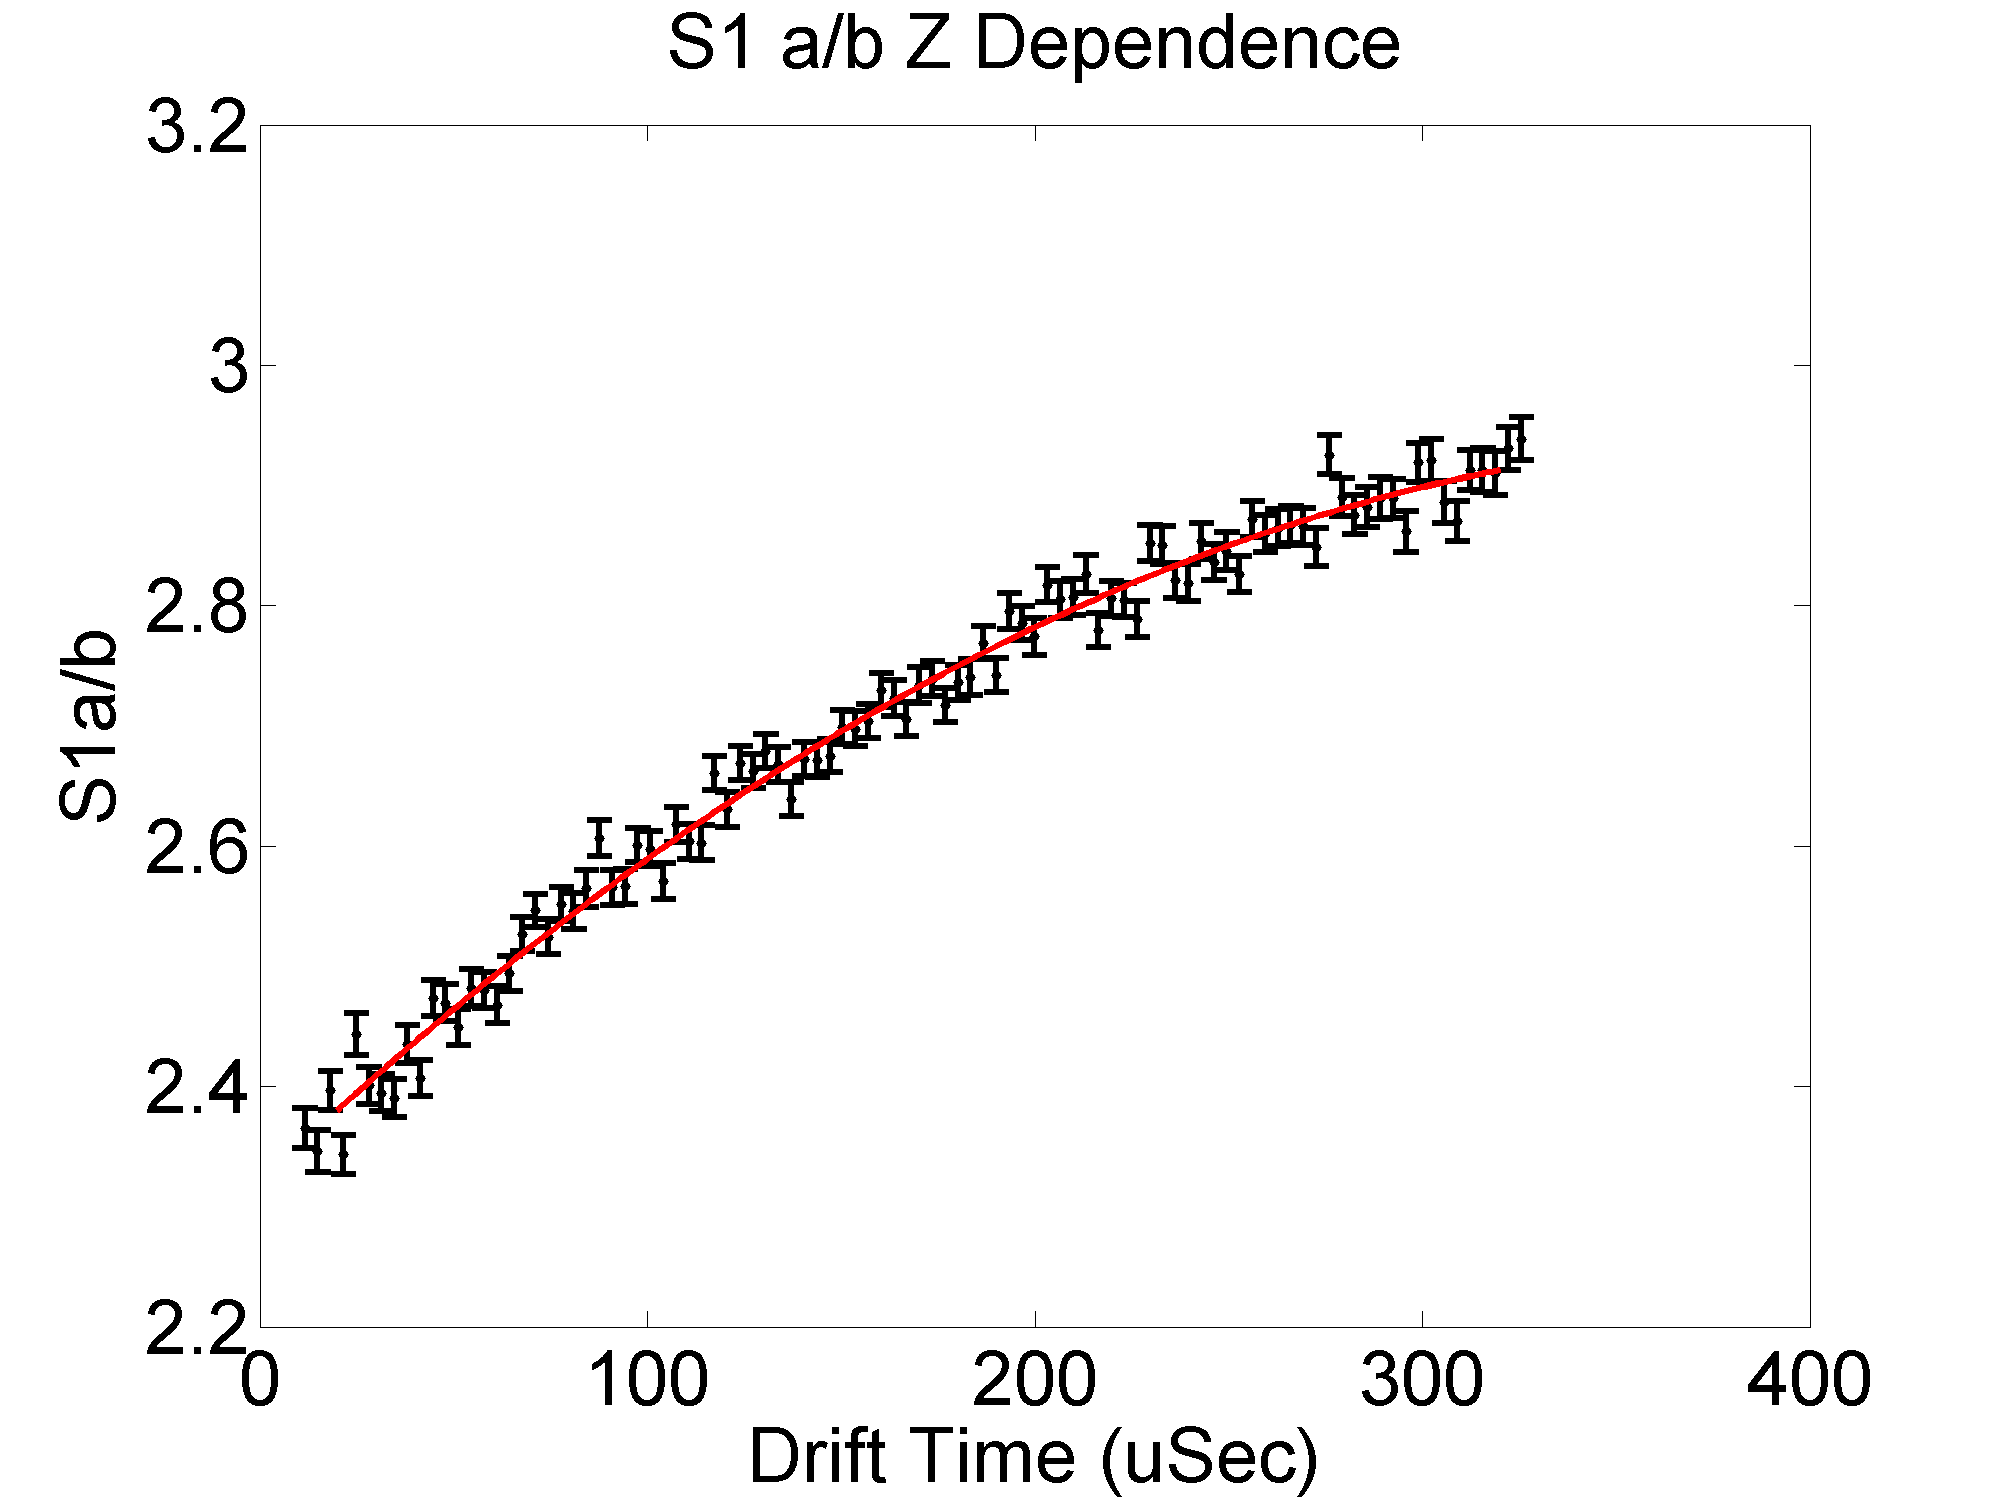
\includegraphics[width=6.5cm]{Run04Corrections/S1aS1bZDep.png} }}
\captionof{figure}{ (Left) Gaussian distribution fits to the $^{83m}$Kr S1a data that are used to determine the drift time dependence of the S1a/S1b ratio. For illustrative purposes, a drift time bin width of 60 $\mu$s was chosen for this plot.  Similar fits are performed on the S1b pulse area data. (Right) The Z dependence of the $^{83m}$Kr S1a/S1b ratio.  Black points indicate the S1a/S1b ratio as measured by the Gaussian distribution fits for each drift time bin, and the red line indicates the polynomial fit to this data.  Data from lux10\_20150929T1905\_cp17540.}
\label{fig:S1aGaussianPlot}
\end{figure}

The XY dependence $^{83m}$Kr S1a/S1b signal is found in a similar manner.  We first remove the z dependence of the S1a/S1b data by normalizing the polynomial fit found above to the detector center (defined by taking the mean drift time value of all $^{83m}$Kr events above 4 $\mu$s drift time). We then divide the detector into two dimensional XY bins with lengths of 3 cm on each side and fit a Gaussian distribution to the S1a and S1b data of each bin.  The mean of the Gaussian distribution from each bin is used to construct an S1a/S1b XY dependence map, with a spline interpolation and extrapolation being used to determine the XY dependence between and outside of the bins. (Figure \ref{fig:S1aS1bXYDep})  Both the one dimensional (Z) and three dimensional methods will be used latter in the analysis, with close agreement between either method.


We also take a separate, three dimensional approach to mapping the $^{83m}$Kr S1a/S1b ratio throughout the detector. In this approach the detector is divided into three dimensional voxels, with X and Y width of 3.5 cm and Z width of 30 $\mu$s.  A three dimensional map of S1a/S1b is produced by fitting a Gaussian distribution to the S1a and S1b pulse area spectrum in each voxel.  A spline interpolation and extrapolation is used to determine the S1a/S1b ratio between and outside of the three dimensional voxels.

\begin{figure}[!h]
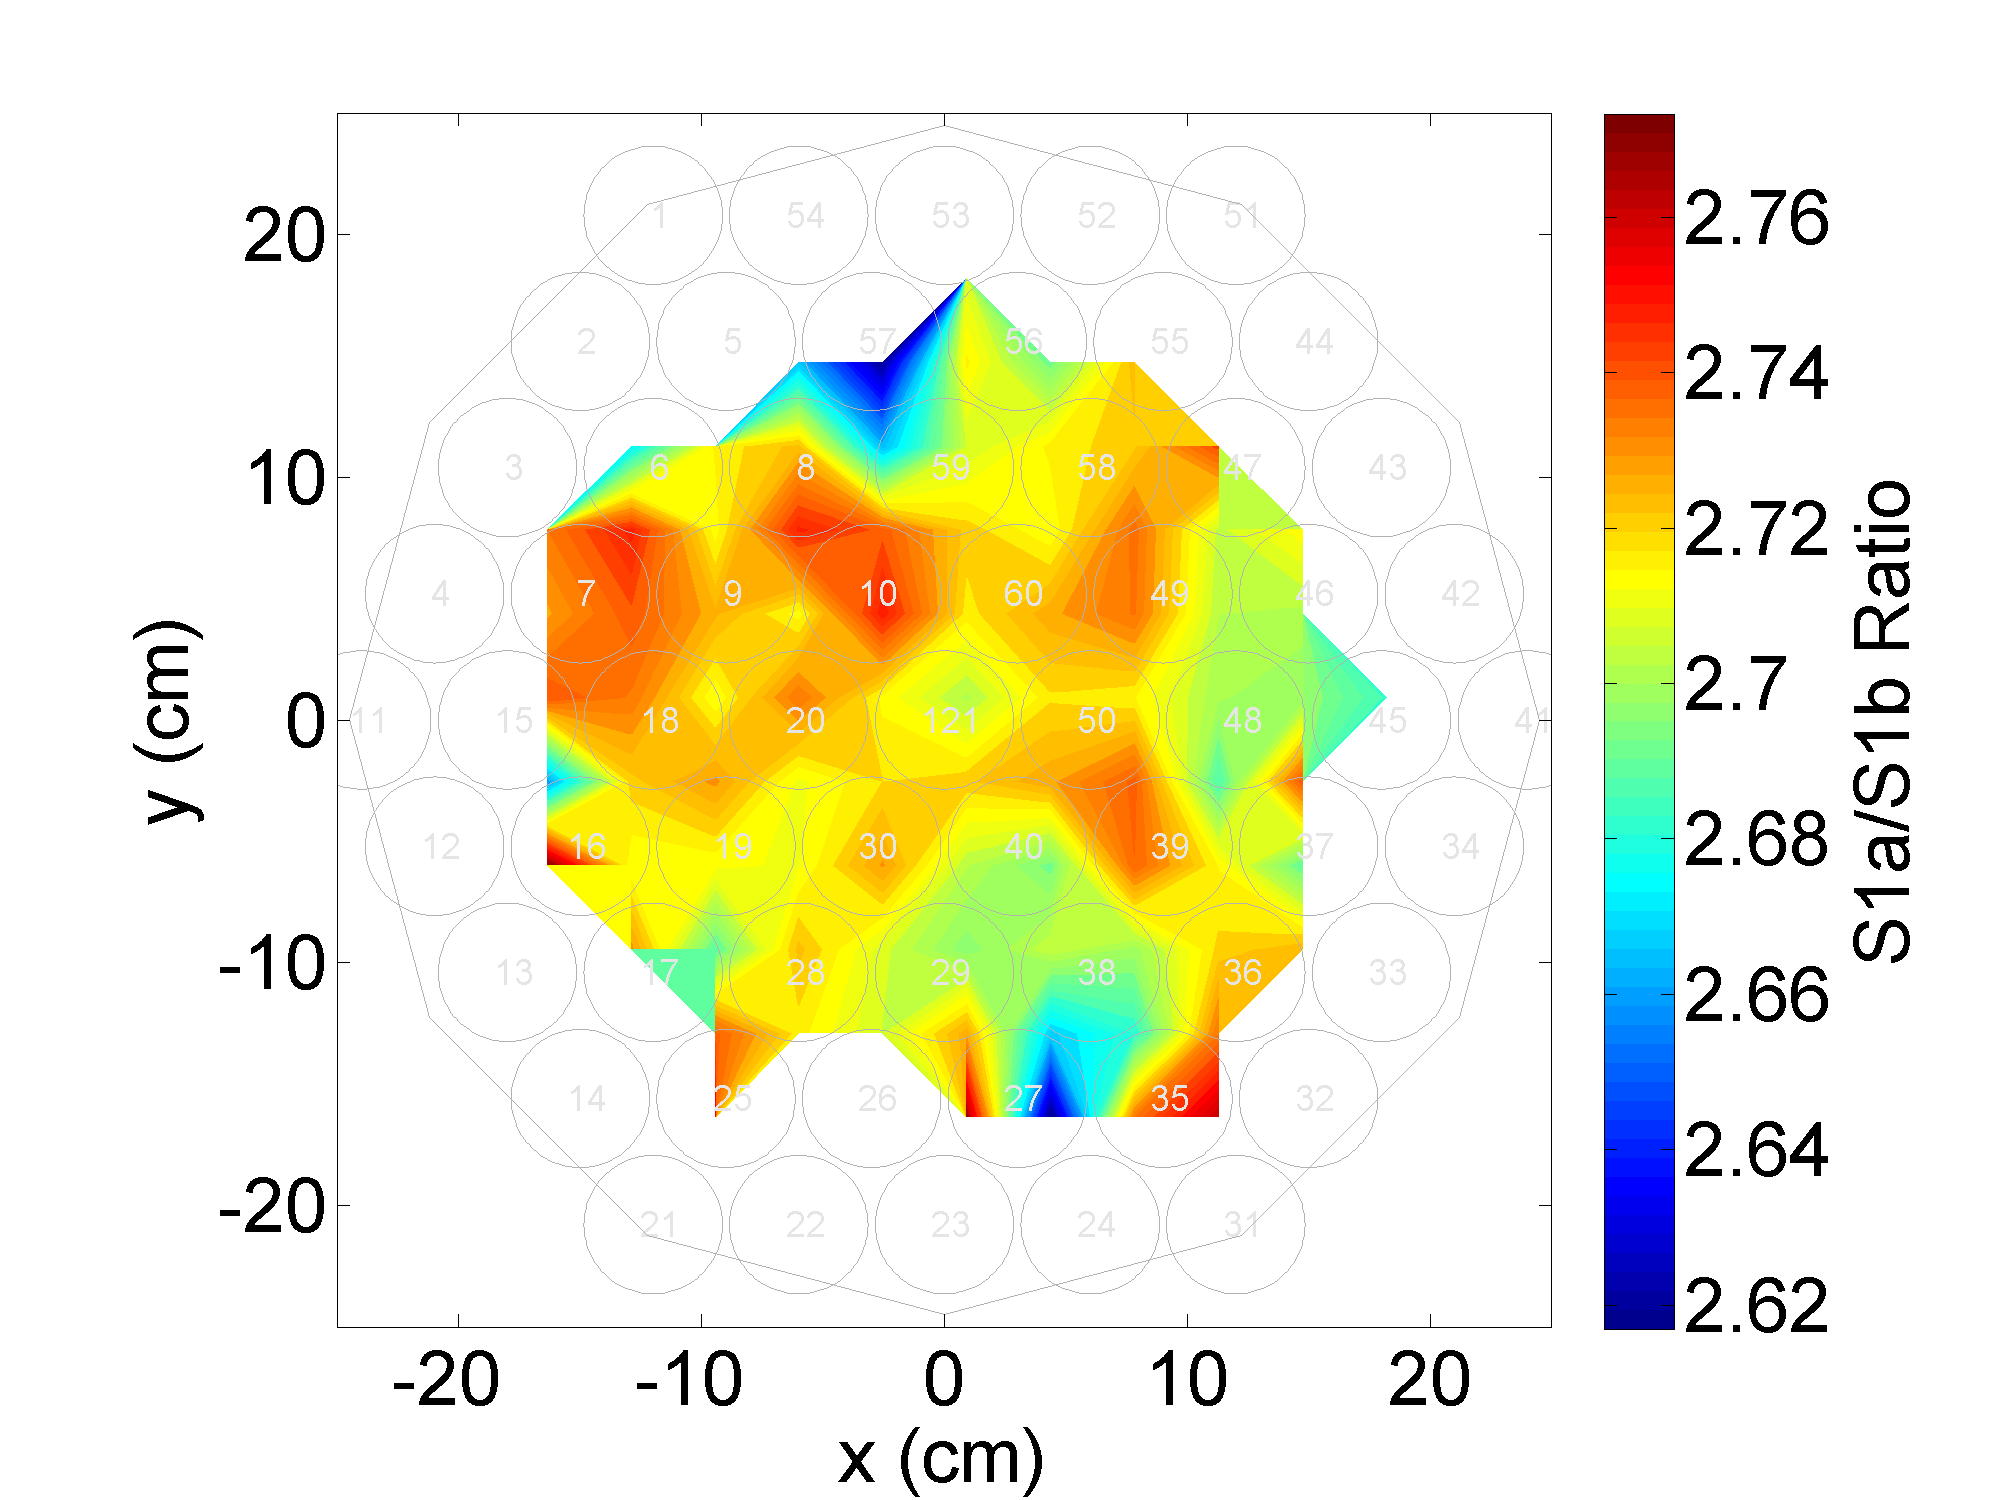
\includegraphics[scale=0.6]{Run04Corrections/S1aS1bvXY.png}
\captionof{figure}{The XY dependence of the $^{83m}$Kr S1a/S1b ratio determined by fitting a Gaussian distribution to XY bins of the S1a and S1b data and tracking the mean of each fit.  The map does not extend to r=25 cm due to the squeezing effect of the nonuniform electric field. Data from lux10\_20150929T1905\_cp17540.}
 \label{fig:S1aS1bXYDep}
\end{figure}

Finally, we relate the Z dependence, XY dependence, and three dimensional dependence maps of the S1a/S1b ratio to the Z dependence, XY dependence, and three dimensional dependence maps of the S2 field effect measured in section \ref{section:FieldEffects}.  We choose to discard the XY dependence maps since no significant relationship is found between them. (Figure \ref{fig:S1aS1bField_S2XY}) This lack of correlation is attributed to the Z dependence of the electric field being much more dominant than the XY dependence of the electric field.  

%Note.. when calculating errors, outcome of polynomial was slightly diferent from first time around due to changing in 1D interp code.  Used same fractional size of errors for the errors here

A second order polynomial is fit to the spatial dependence of the $^{83m}$Kr S2$_E$ (induced by the field effect) to S1a/S1b relationship, with best fit parameters of $a=-0.499 \pm 0.117$,$b=1.48 \pm 0.615$, and $c=0.667 \pm 0.946$ for the second order, first order, and zeroth order terms, respectively.  This polynomial will be used in KrypCal to determine the strength of the field effect in $^{83m}$Kr S2 data at all points in time.  We find that the Z dependence and three dimensional maps agree closely within the range of measured S1a/S1b ratios, but begin to diverge in the extrapolated regions. (Figure \ref{fig:S1aS1bField_S2})  Because the electric field varies more in September 2015 than at earlier times in Run4, and because the time variation of the electric field has significantly slowed at times later than September 2015, we expect the measured range of S1a/S1b ratios in this work will cover the majority of S1a/S1b ratios that will ever be measured in Run4. Therefore, the discrepancy in the extrapolation of each map is not concerning. 

\begin{figure}[!h]
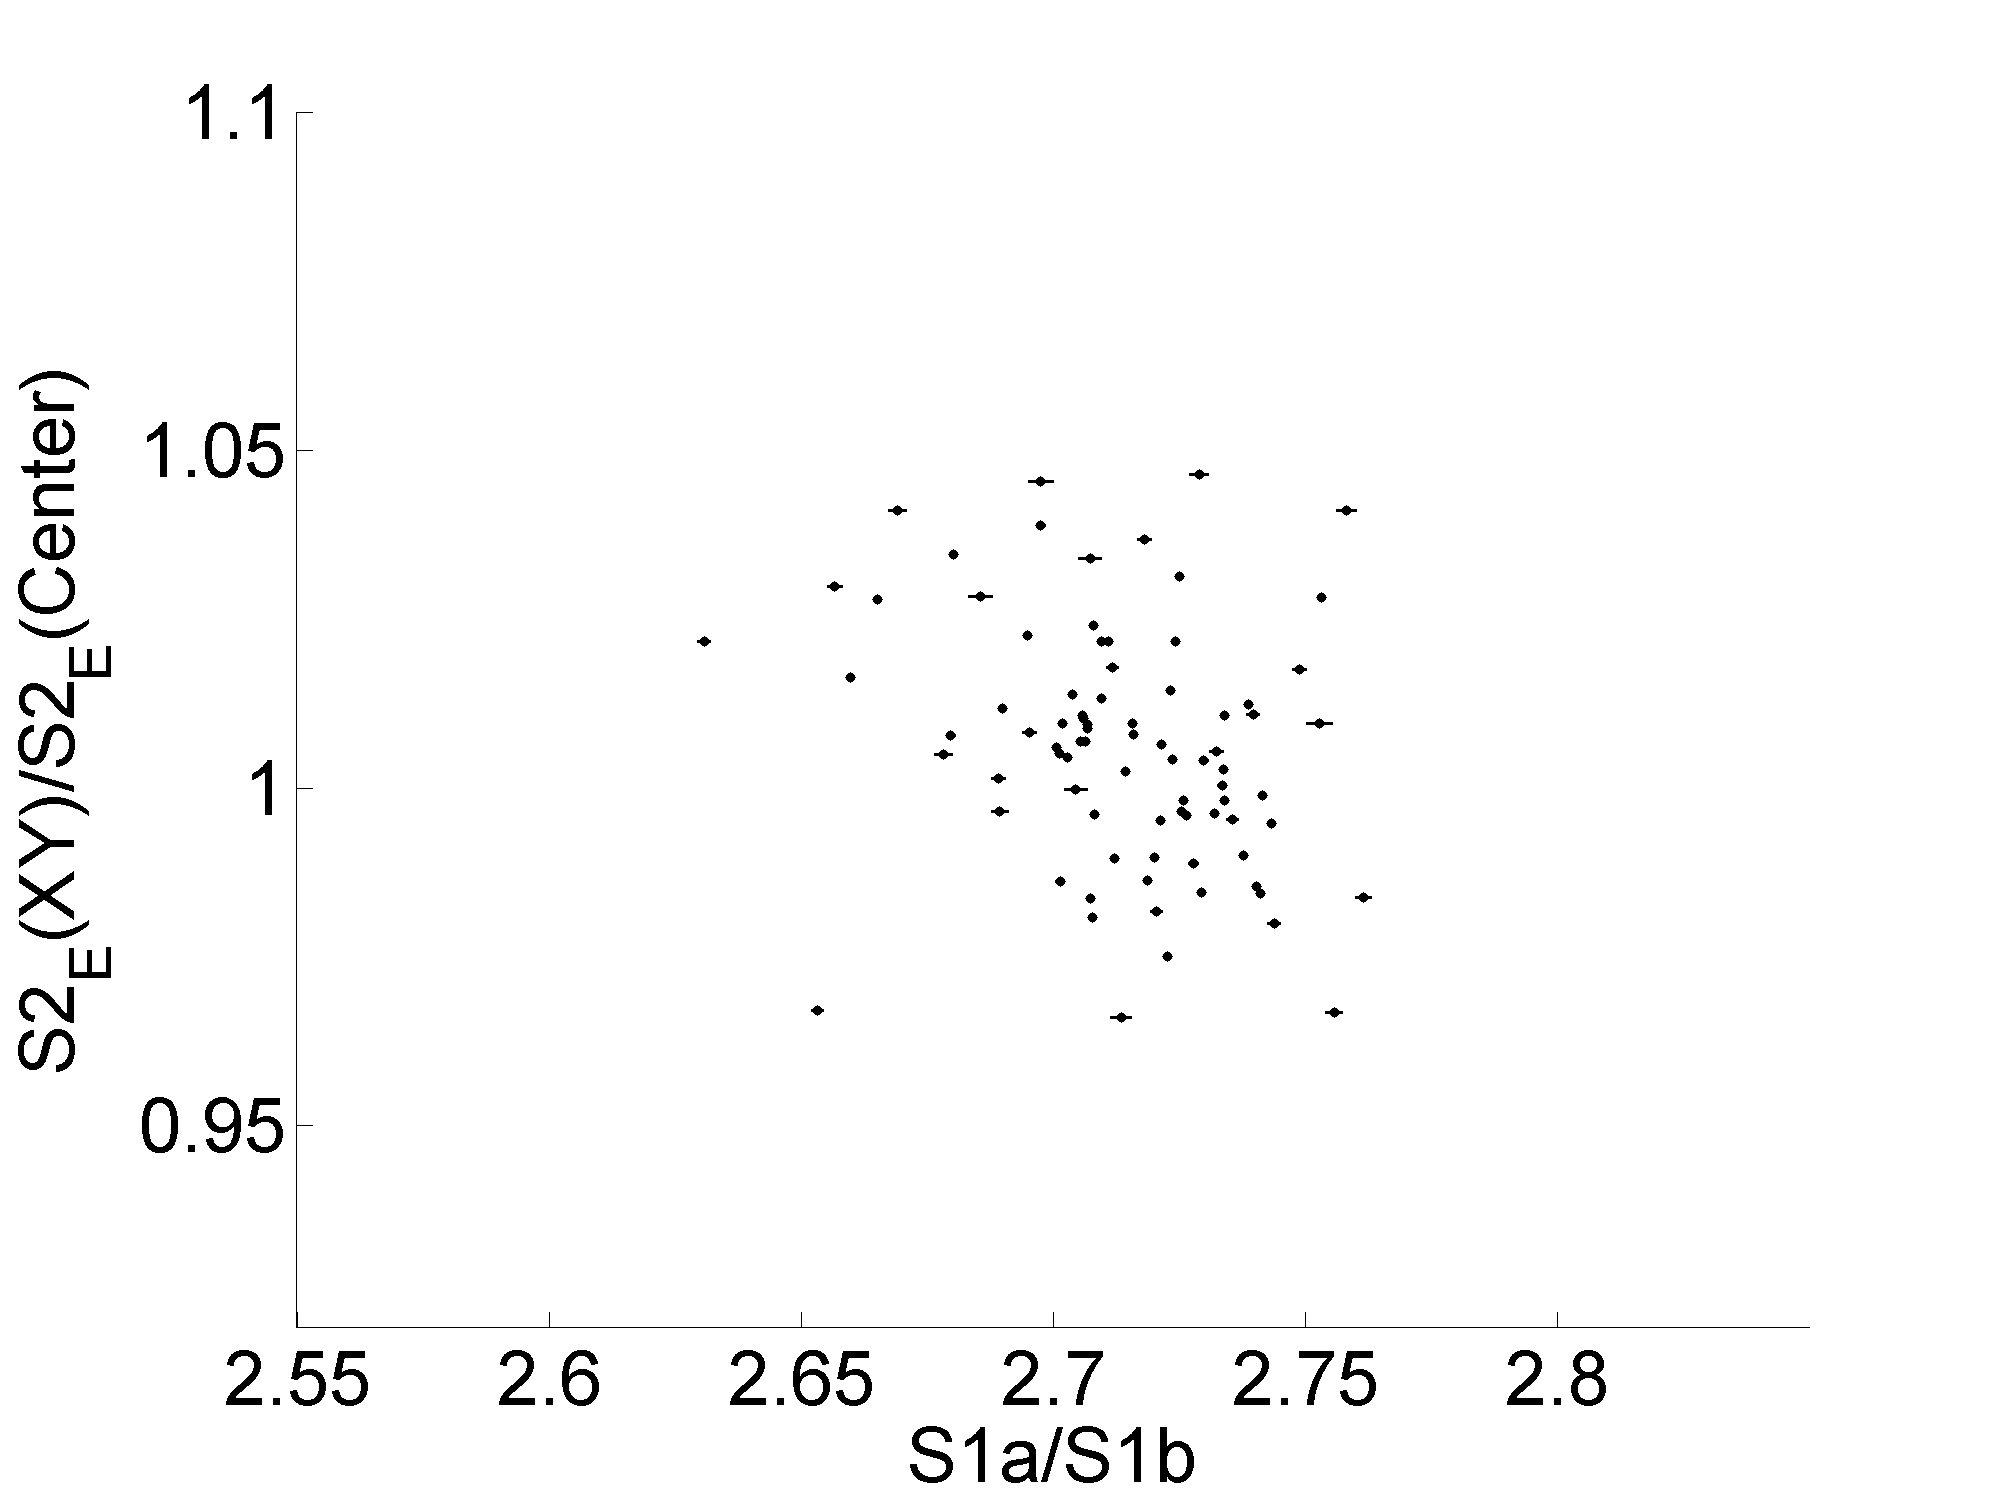
\includegraphics[scale=0.6]{Run04Corrections/S1aS1bVField_XYDep.png}
\captionof{figure}{The XY relationship of the $^{83m}$Kr S1a/S1b ratio to the $^{83m}$Kr S2$_E$ field effect in lux10\_20150929T1905\_cp17540.  A low correlation coefficient of 0.26 is found in this data.}
 \label{fig:S1aS1bField_S2XY}
\end{figure}

\begin{figure}[!h]
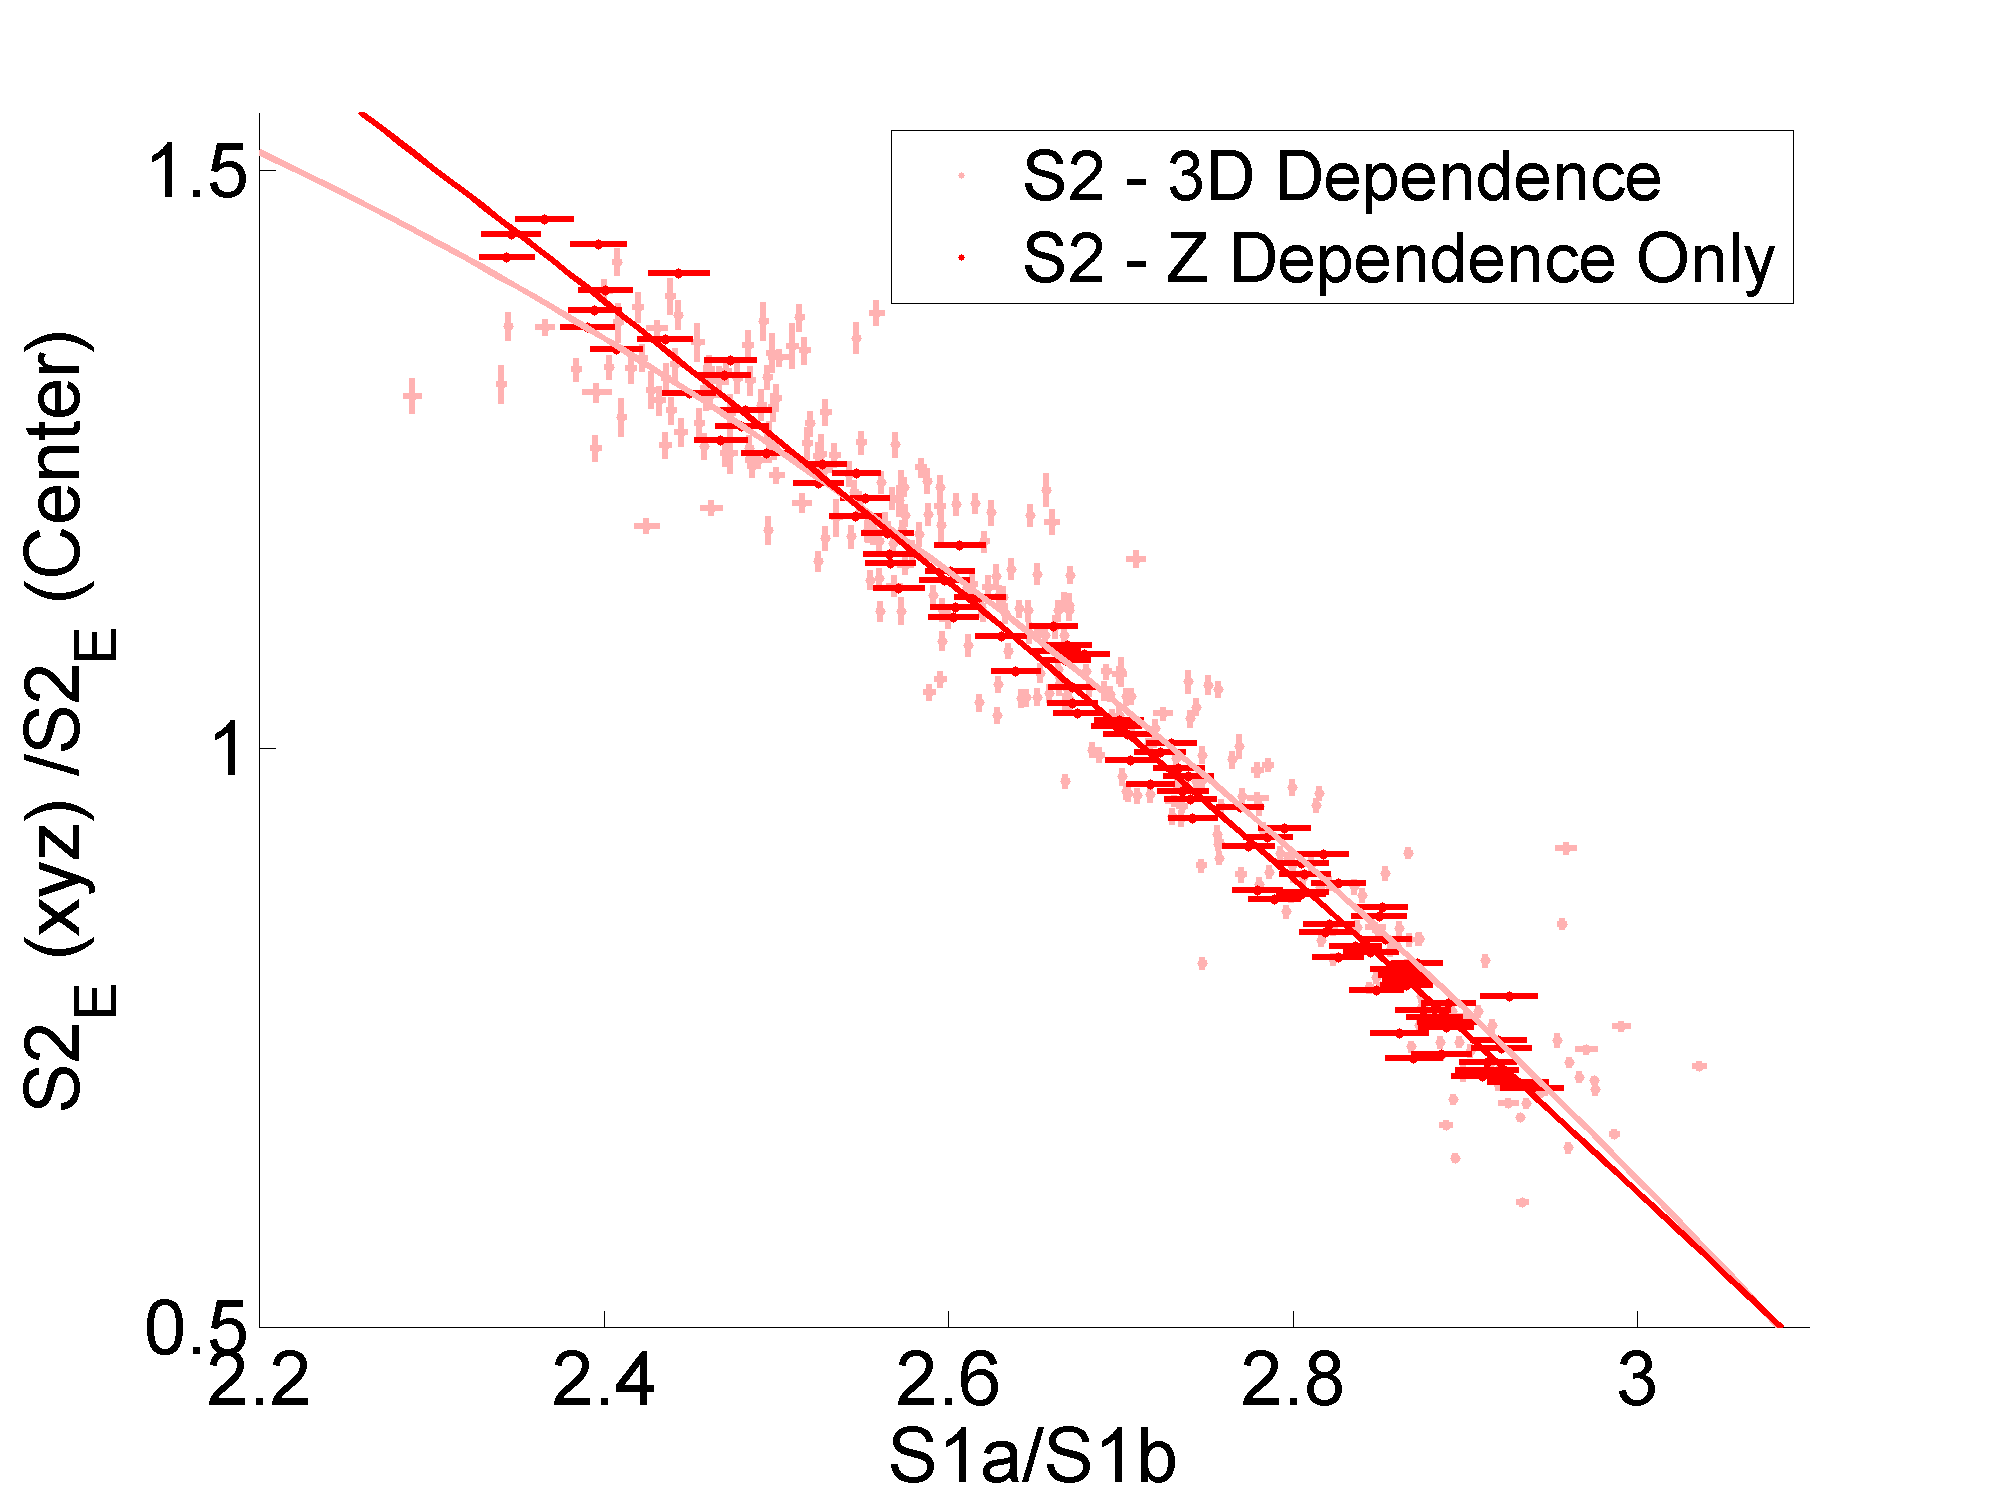
\includegraphics[scale=0.6]{Run04Corrections/S1aS1bvField_ZDep_3D_S2Only.png}
\captionof{figure}{The Z (dark red) and three dimensional (light red) relationship of the $^{83m}$Kr S1a/S1b ratio to the $^{83m}$Kr S2$_E$ field effect.}
 \label{fig:S1aS1bField_S2}
\end{figure}


\subsubsection{Measuring the S1a/S1b Ratio to S1 Field Effect Relationship with Recombination Physics} \label{section:S1relation}

We have successfully measured the strength of the field effect in $^{83m}$Kr S2 data at one point in time, and have related it to the $^{83m}$Kr S1a/S1b ratio such that we can determine the strength of the field effect at any point in time.  We are now left with the challenge of measuring the strength of the field effect in $^{83m}$Kr S1 data. Our first approach will turn to the recombination physics that governs particle interaction during a recoil event.  

%NOTE: THIS IS USING THE INVERSE OF THE 10212015 COLLAB TALK EQUATIONS, WHICH DEFINE THE FIELD CORRECTION FACTOR
The strength of the field effect (normalized to the detector center) in $^{83m}$Kr S2 data is given by the ratio of the inefficiency corrected S2$_E$ at a given position to the inefficiency corrected S2$_E$ at the center of the detector, which was measured in \ref{section:FieldEffects}.  This ratio can be written in terms of the recombination during a $^{83m}$Kr event ($R_{Kr}$) as follows
\begin{equation}
\frac{S2_{E,Kr}(xyz)}{S2_{E,Kr}(center)} = \frac{1-R_{Kr}(xyz)}{1-R_{Kr}(center)}
\end{equation}
Note that this can be rewritten as an expression for the recombination during a $^{83m}$Kr as a function of position,
\begin{equation} \label{RKr}
R_{Kr}(xyz) = 1- \frac{S2_{E,Kr}(xyz)}{S2_{E,Kr}(center)}(1-R_{Kr}(center)).
\end{equation}
Next, we write the strength of the field effect in $^{83m}$Kr S1 data (normalized to the detector center) as the ratio of the inefficiency corrected S1$_E$ signal at a given position to the inefficiency corrected S1$_E$ signal at the center of the detector, which we are unable to measure directly.  In terms of the exciton to ion ratio ($\alpha$) and the recombination during a $^{83m}$Kr event ($R_{Kr}$) this is given by 
\begin{equation} \label{S1fieldstrength}
\frac{S1_{E,Kr}(xyz)}{S1_{E,Kr}(center)}=\frac{\alpha+R_{Kr}(xyz)}{\alpha+R_{Kr}(center)} = \frac{\alpha + 1 - \frac{S2_{E,Kr}(xyz)}{S2_{E,Kr}(center)}(1-R_{Kr}(center))}{\alpha + R_{Kr}(center)}
\end{equation}
where we have used equation \ref{RKr} in the last step.  Therefore, all we need to measure the strength of the field effect on $^{83m}$Kr S1 data is the recombination during a $^{83m}$Kr event at the center of the detector, given by $R_{Kr}(center)$.  As mentioned in section \ref{section:GenStrat}, NEST does not simulate the physics of $^{83m}$Kr events well, but it has been tuned to simulate the physics of CH$_3$T events.  As such, we once again turn to the CH$_3$T data to determine the value of $R_{Kr}(center)$.  First, we write the ratio of the efficiency corrected $^{83m}$Kr  S2$_E$ pulse area at the center of the detector to the efficiency corrected CH$_3$T S2$_E$ pulse are at the center of the detector in terms of the S2 gain factor ($g_2$), recombination during a $^{83m}$Kr event ($R_{Kr}$), recombination during a CH$_3$T event ($R_{H3}$), number of ions produced during a $^{83m}$Kr event ($N_{ion-Kr}$), and number of ions produced during a CH$_3$T event ($N_{ion-H3}$), given by
\begin{equation}
\frac{S2_{E,Kr}(center)}{S2_{E,H3}(center)} = \frac{g_2(1-R_{Kr}(center))N_{ion-Kr}}{g_2(1-R_{H3}(center))N_{ion-H3}}.
\end{equation}
This can be rewritten as an expression for the recombination of $^{83m}$Kr at the center of the detector given by
\begin{equation} \label{RKr_cent}
R_{Kr}(center)=1-\frac{S2_{E,Kr}(center)}{S2_{E,H3}(center)}\frac{N_{ion-H3}}{N_{ion_Kr}}(1-R_{H3}(center))
\end{equation}
where the gain factor $g_2$ does not depend on energy, and therefore can be removed from the equation.  The number of ions for both $^{83m}$Kr events and CH$_3$T events is given by equations \ref{NqEq} and \ref{NionEq}, with the assumption $E=41.55$ keV for $^{83m}$Kr and $E=2.5$ keV for CH$_3$T, and the recombination at the center of the detector of CH$_3$T events ($R_{H3}$) can be determined from NEST.

Using equations \ref{S1fieldstrength} and \ref{RKr_cent} we can convert the field effect measured in the $^{83m}$Kr S2$_E$ data to an inferred field effect in $^{83m}$Kr S1 data.
The result of this is shown in Figure \ref{fig:S1FieldFig}.  A $\chi^2$ fit to the expected CH$_3$T and $^{83m}$Kr energy spectra returns an average reduced $\chi^2$ of 1.31, with a reduced $\chi^2$ of 248/124=2.00 for CH$_3$T alone (Figure \ref{ShittyCH3T}), and a reduced $\chi^2$ of 16.2/26=0.622 for $^{83m}$Kr alone using the best fit parameters of $g1=0.1$ and $EE=0.89$.  (Figure \ref{ShittyKr})  It is likely that the complicated nature of the  $^{83m}$Kr decay introduces intricacies which are not account for in equations \ref{S1fieldstrength} and \ref{RKr_cent}.  In the next section we will seek to improve this result with a direct measurement of the S1a/S1b to S1 field effect relationship before turning to a $\chi^2$ minimization method in section \ref{section:S1relation2} to determine the optimal field effect to S1a/S1b relationships.

\begin{figure}[!h]
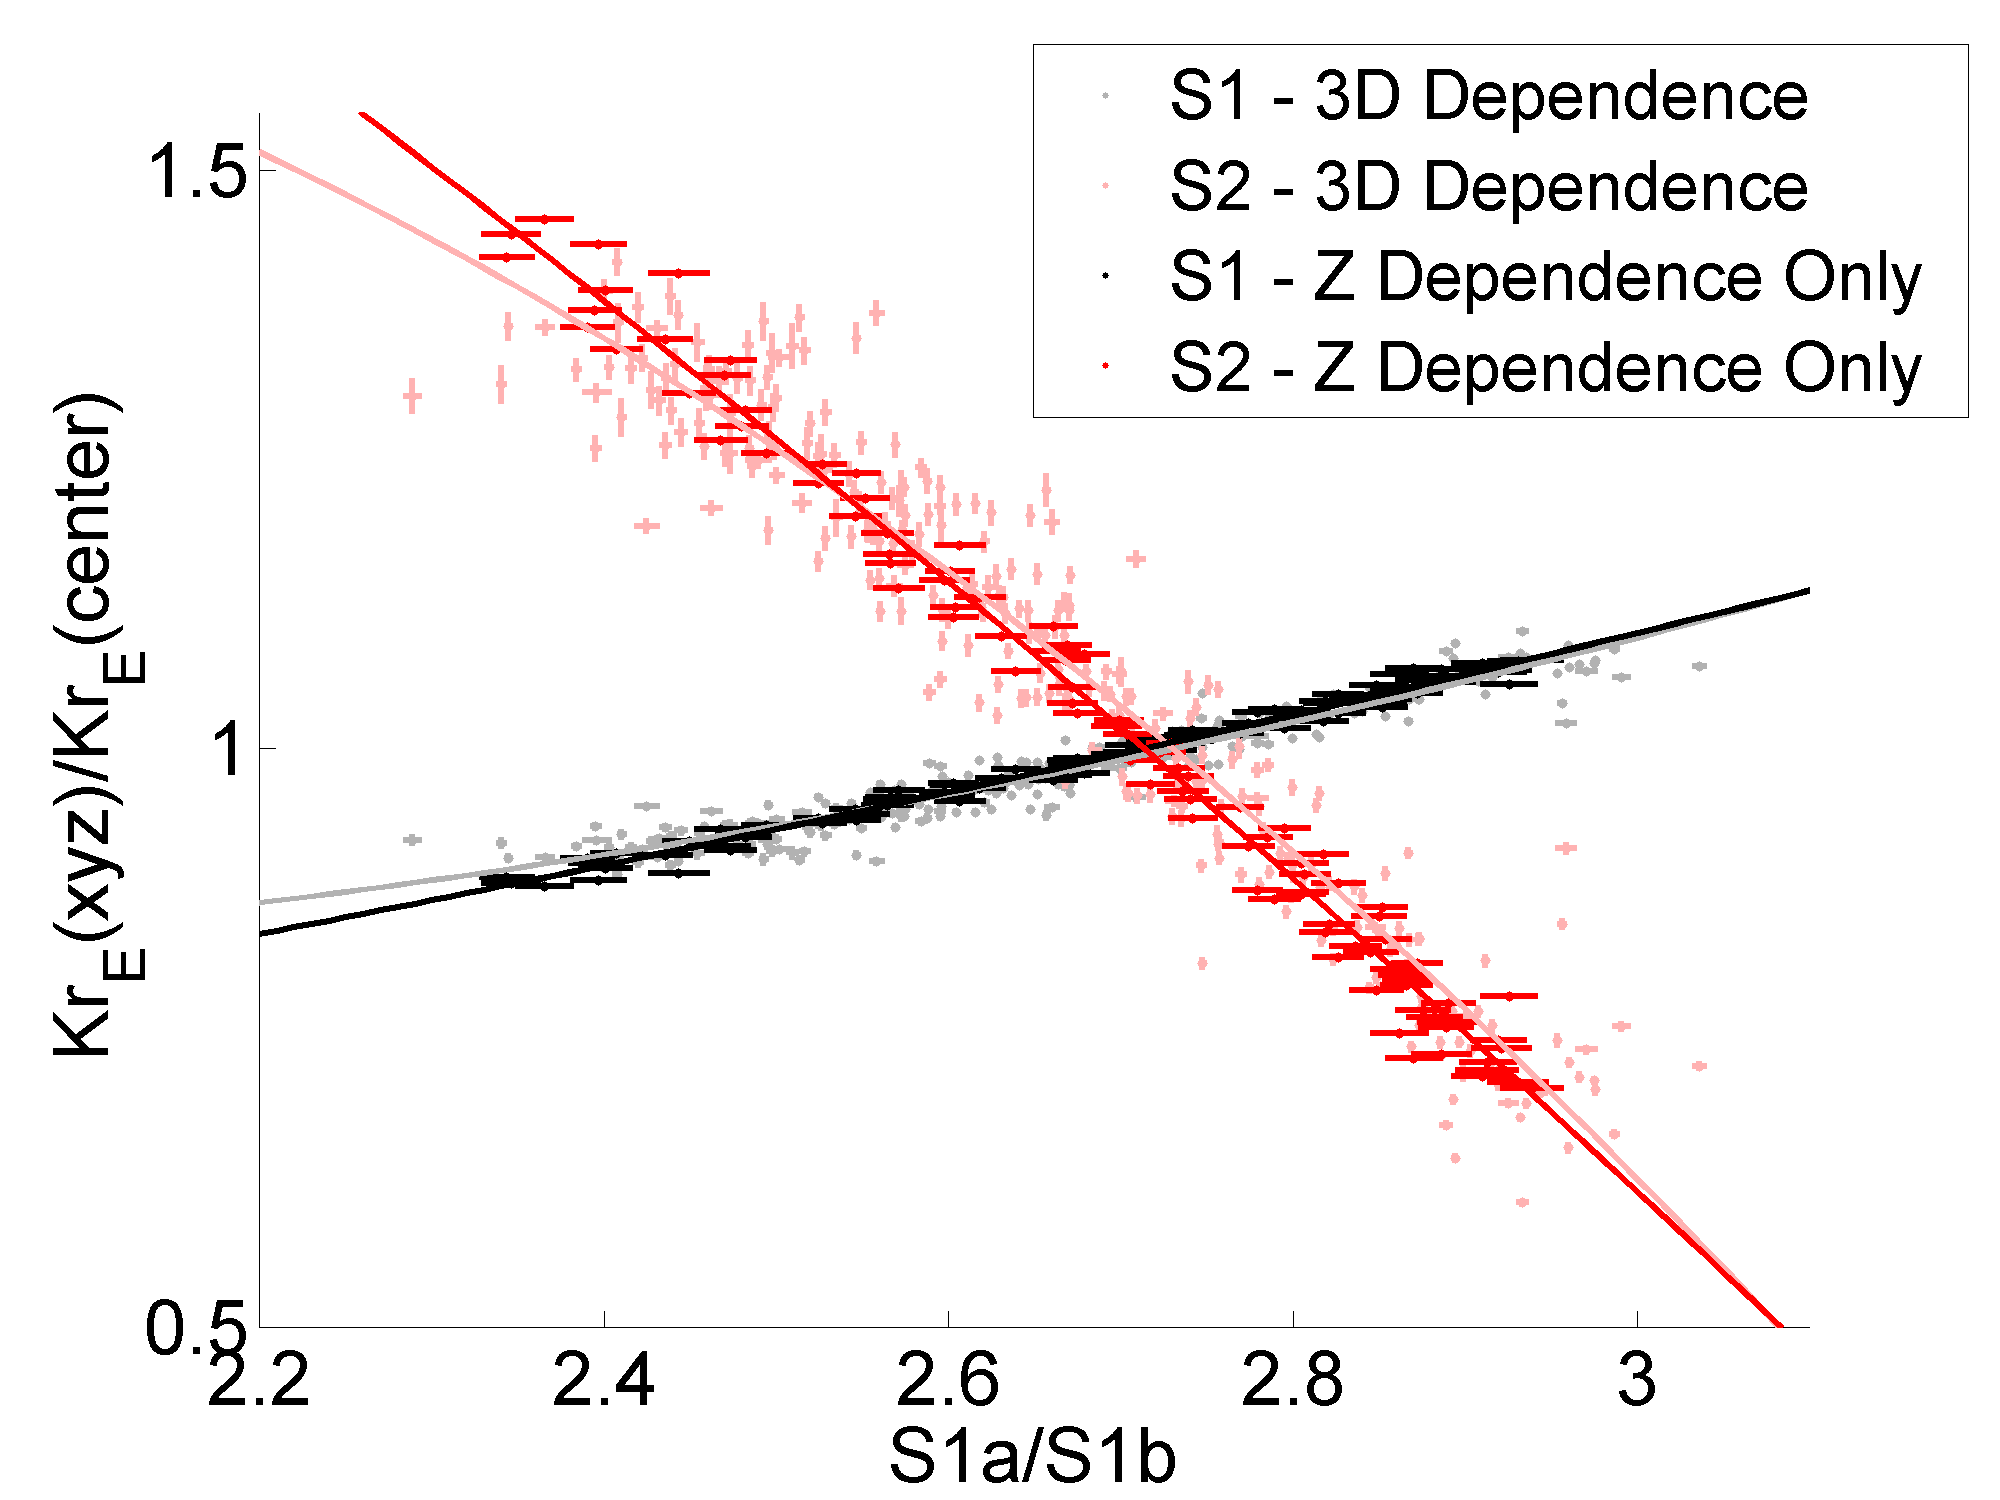
\includegraphics[scale=0.7]{Run04Corrections/S1aS1bvField_ZDep_3D.png}
\captionof{figure}{The Z (black) and three dimensional (grey) relationship of the $^{83m}$Kr S1a/S1b ratio to the $^{83m}$Kr S1 field effect.  The black and grey data points are not measured, but instead inferred from the Z (dark red) and three dimensional (light red) relationship of the $^{83m}$Kr S1a/S1b ratio to the $^{83m}$Kr S2$_E$ field effect.}
 \label{fig:S1FieldFig}
\end{figure}



\begin{figure} [!h]
\centering
\subfloat{{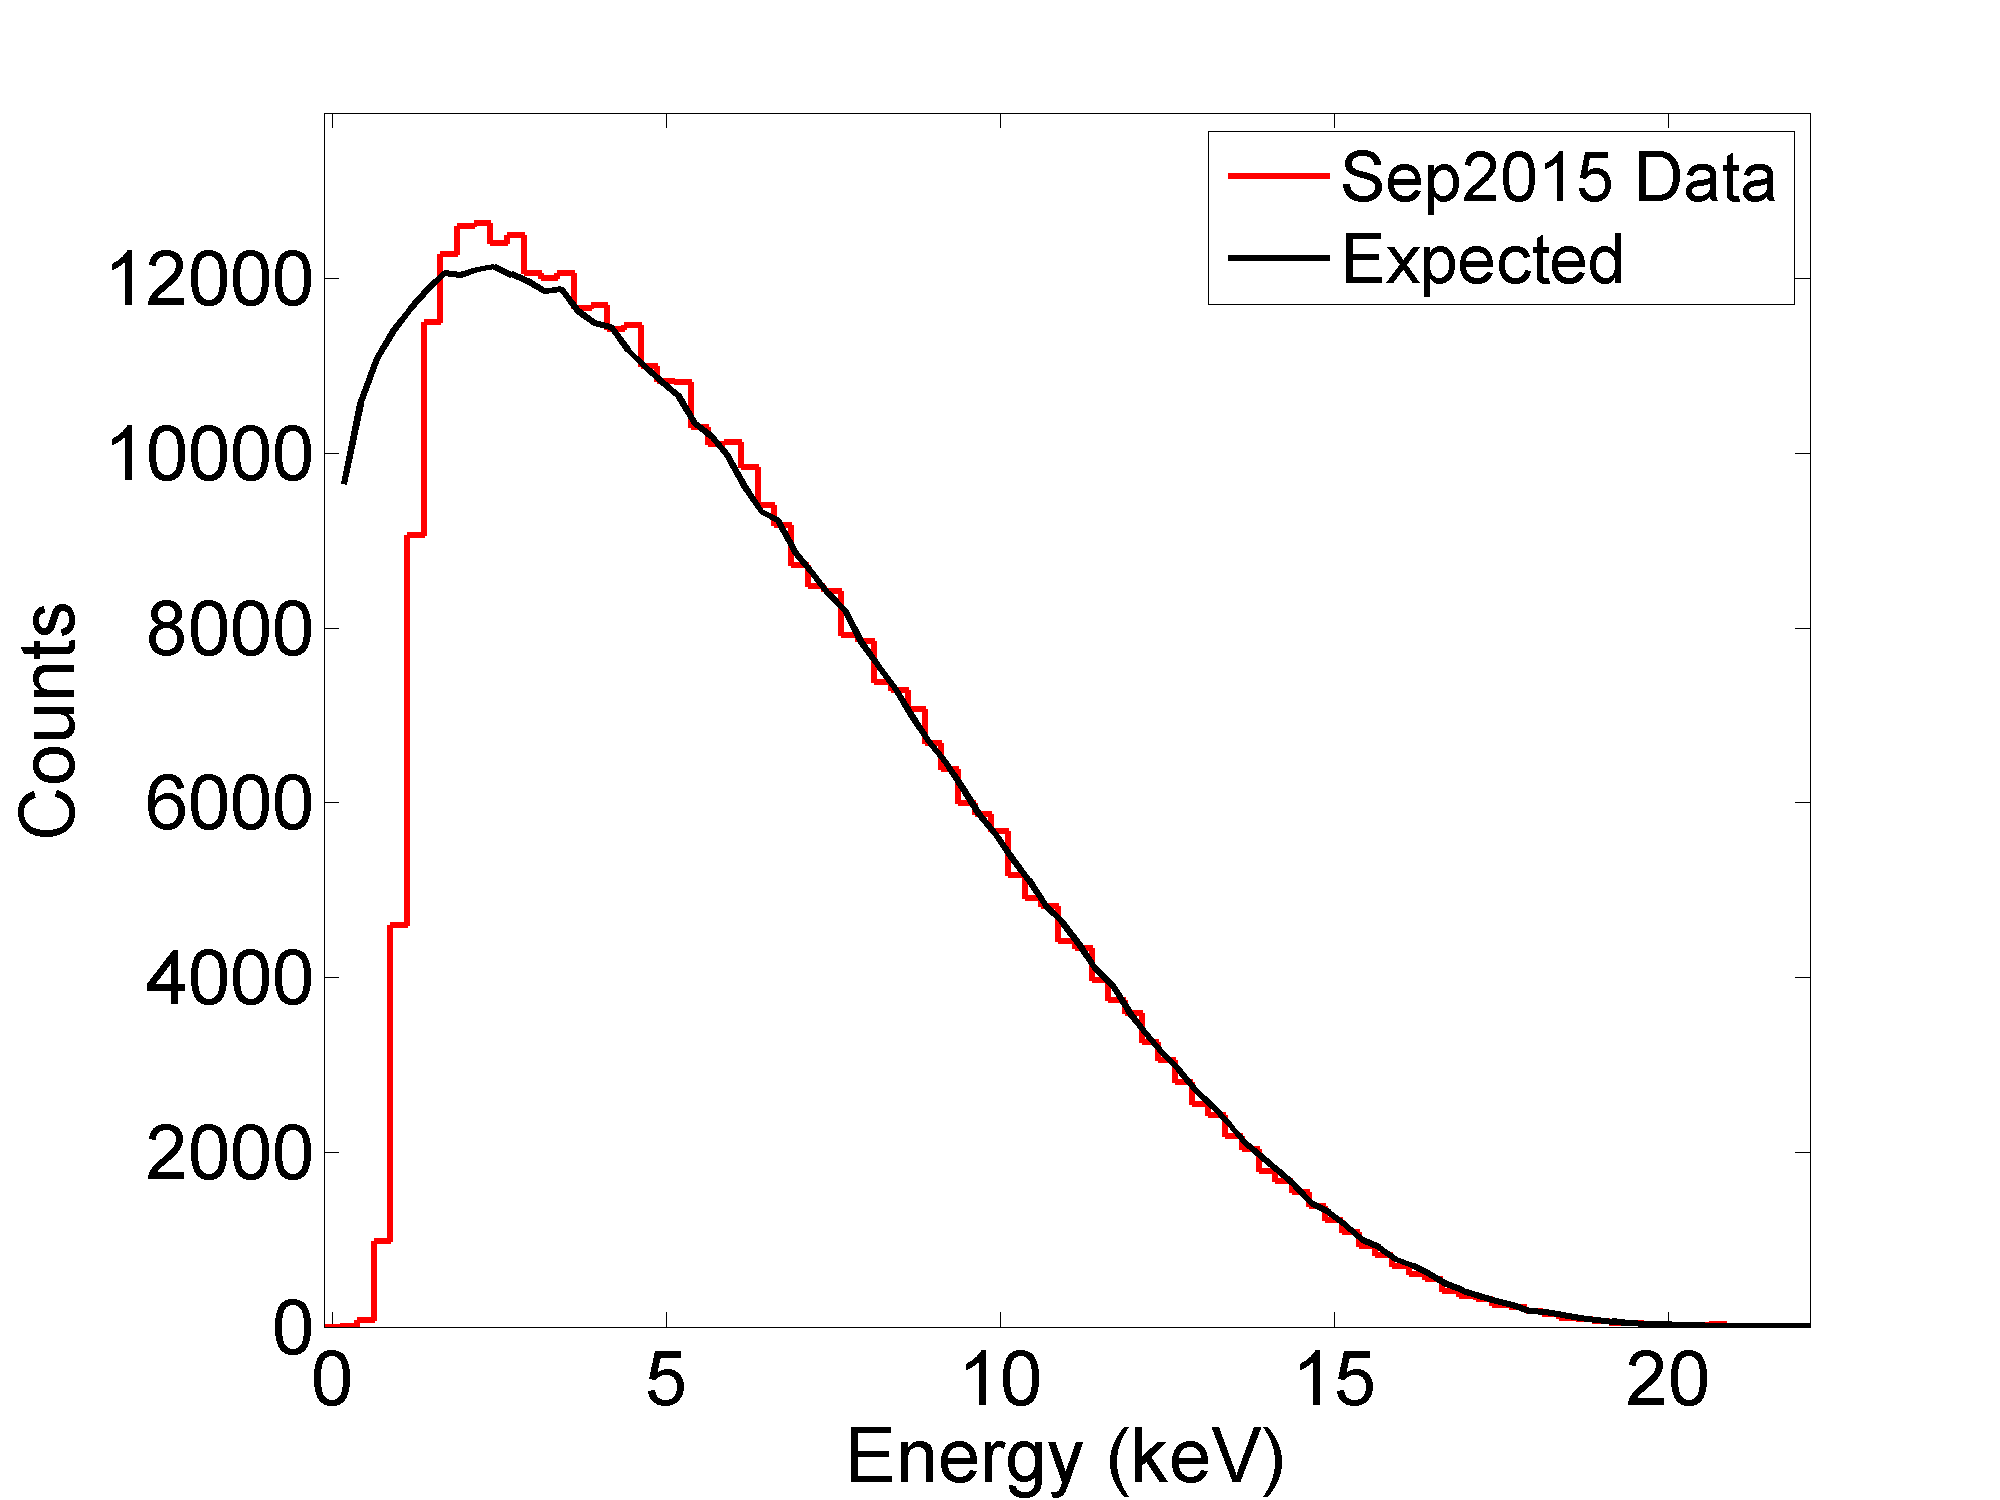
\includegraphics[width=6.5cm]{Run04Corrections/InferredS1Measure_Sep2015CH3T.png} }}
\qquad
\subfloat{{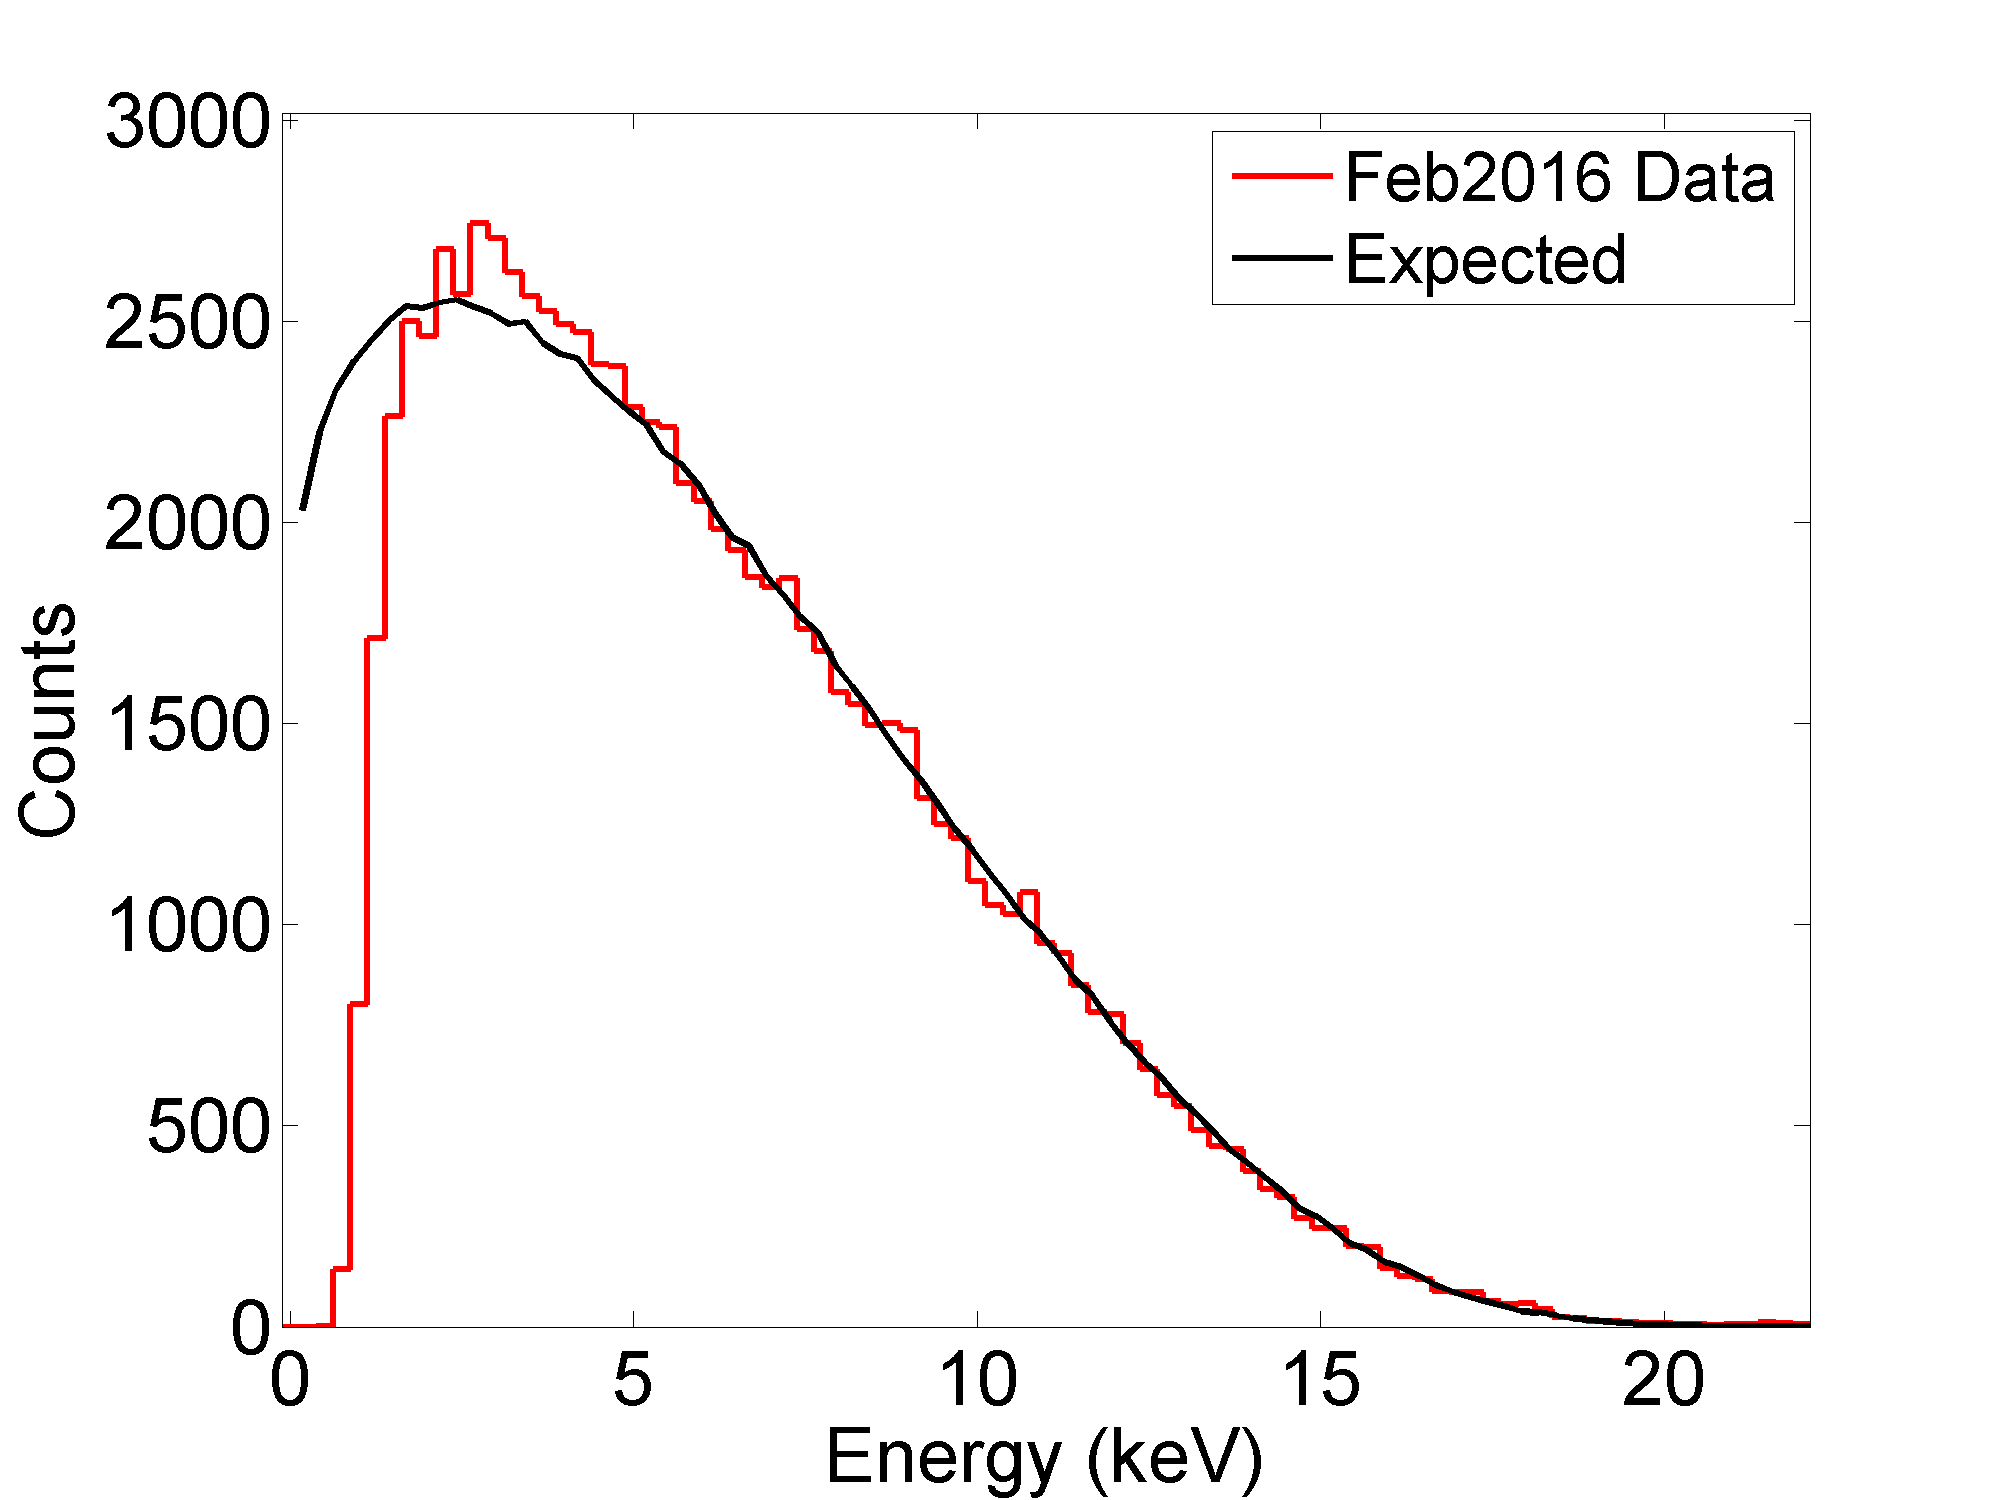
\includegraphics[width=6.5cm]{Run04Corrections/InferredS1Measure_Feb2016CH3T.png} }}
\captionof{figure}{The energy spectrum of the efficiency corrected  CH$_3$T data (red) after utilizing the S1 field effect measurements from this section in September 2015 (left) and February 2016 (right). The expected energy spectrum is shown in black. }
 \label{ShittyCH3T}
\end{figure}


\begin{figure} [!h]
\centering
\subfloat{{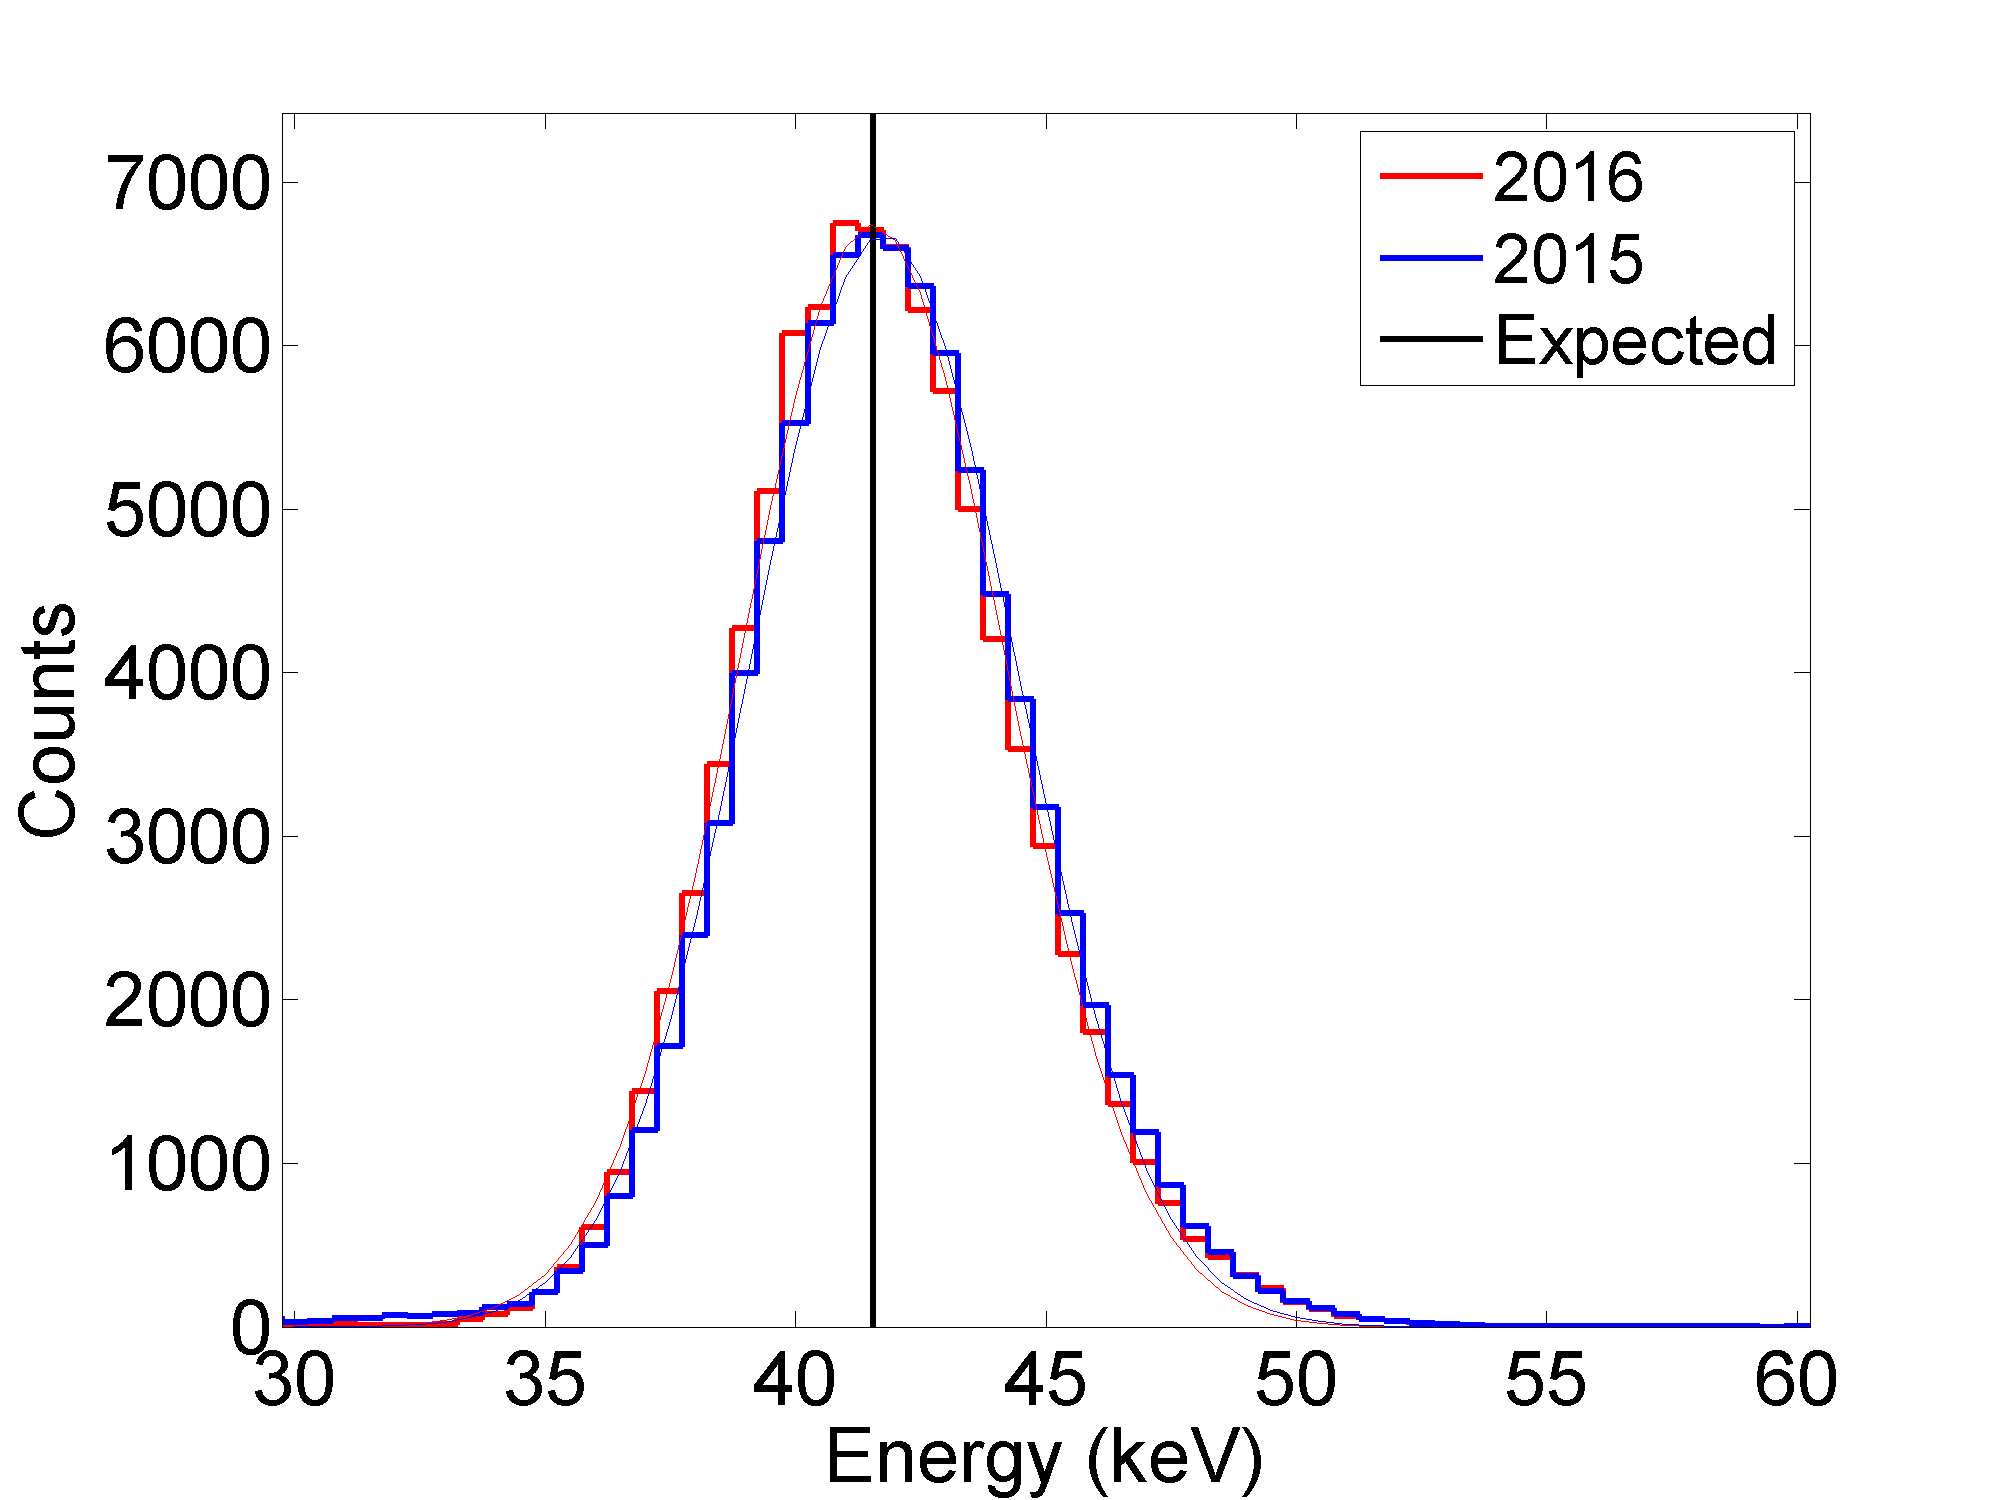
\includegraphics[width=6.5cm]{Run04Corrections/InferredS1Measure_KrSpectra.png} }}
\qquad
\subfloat{{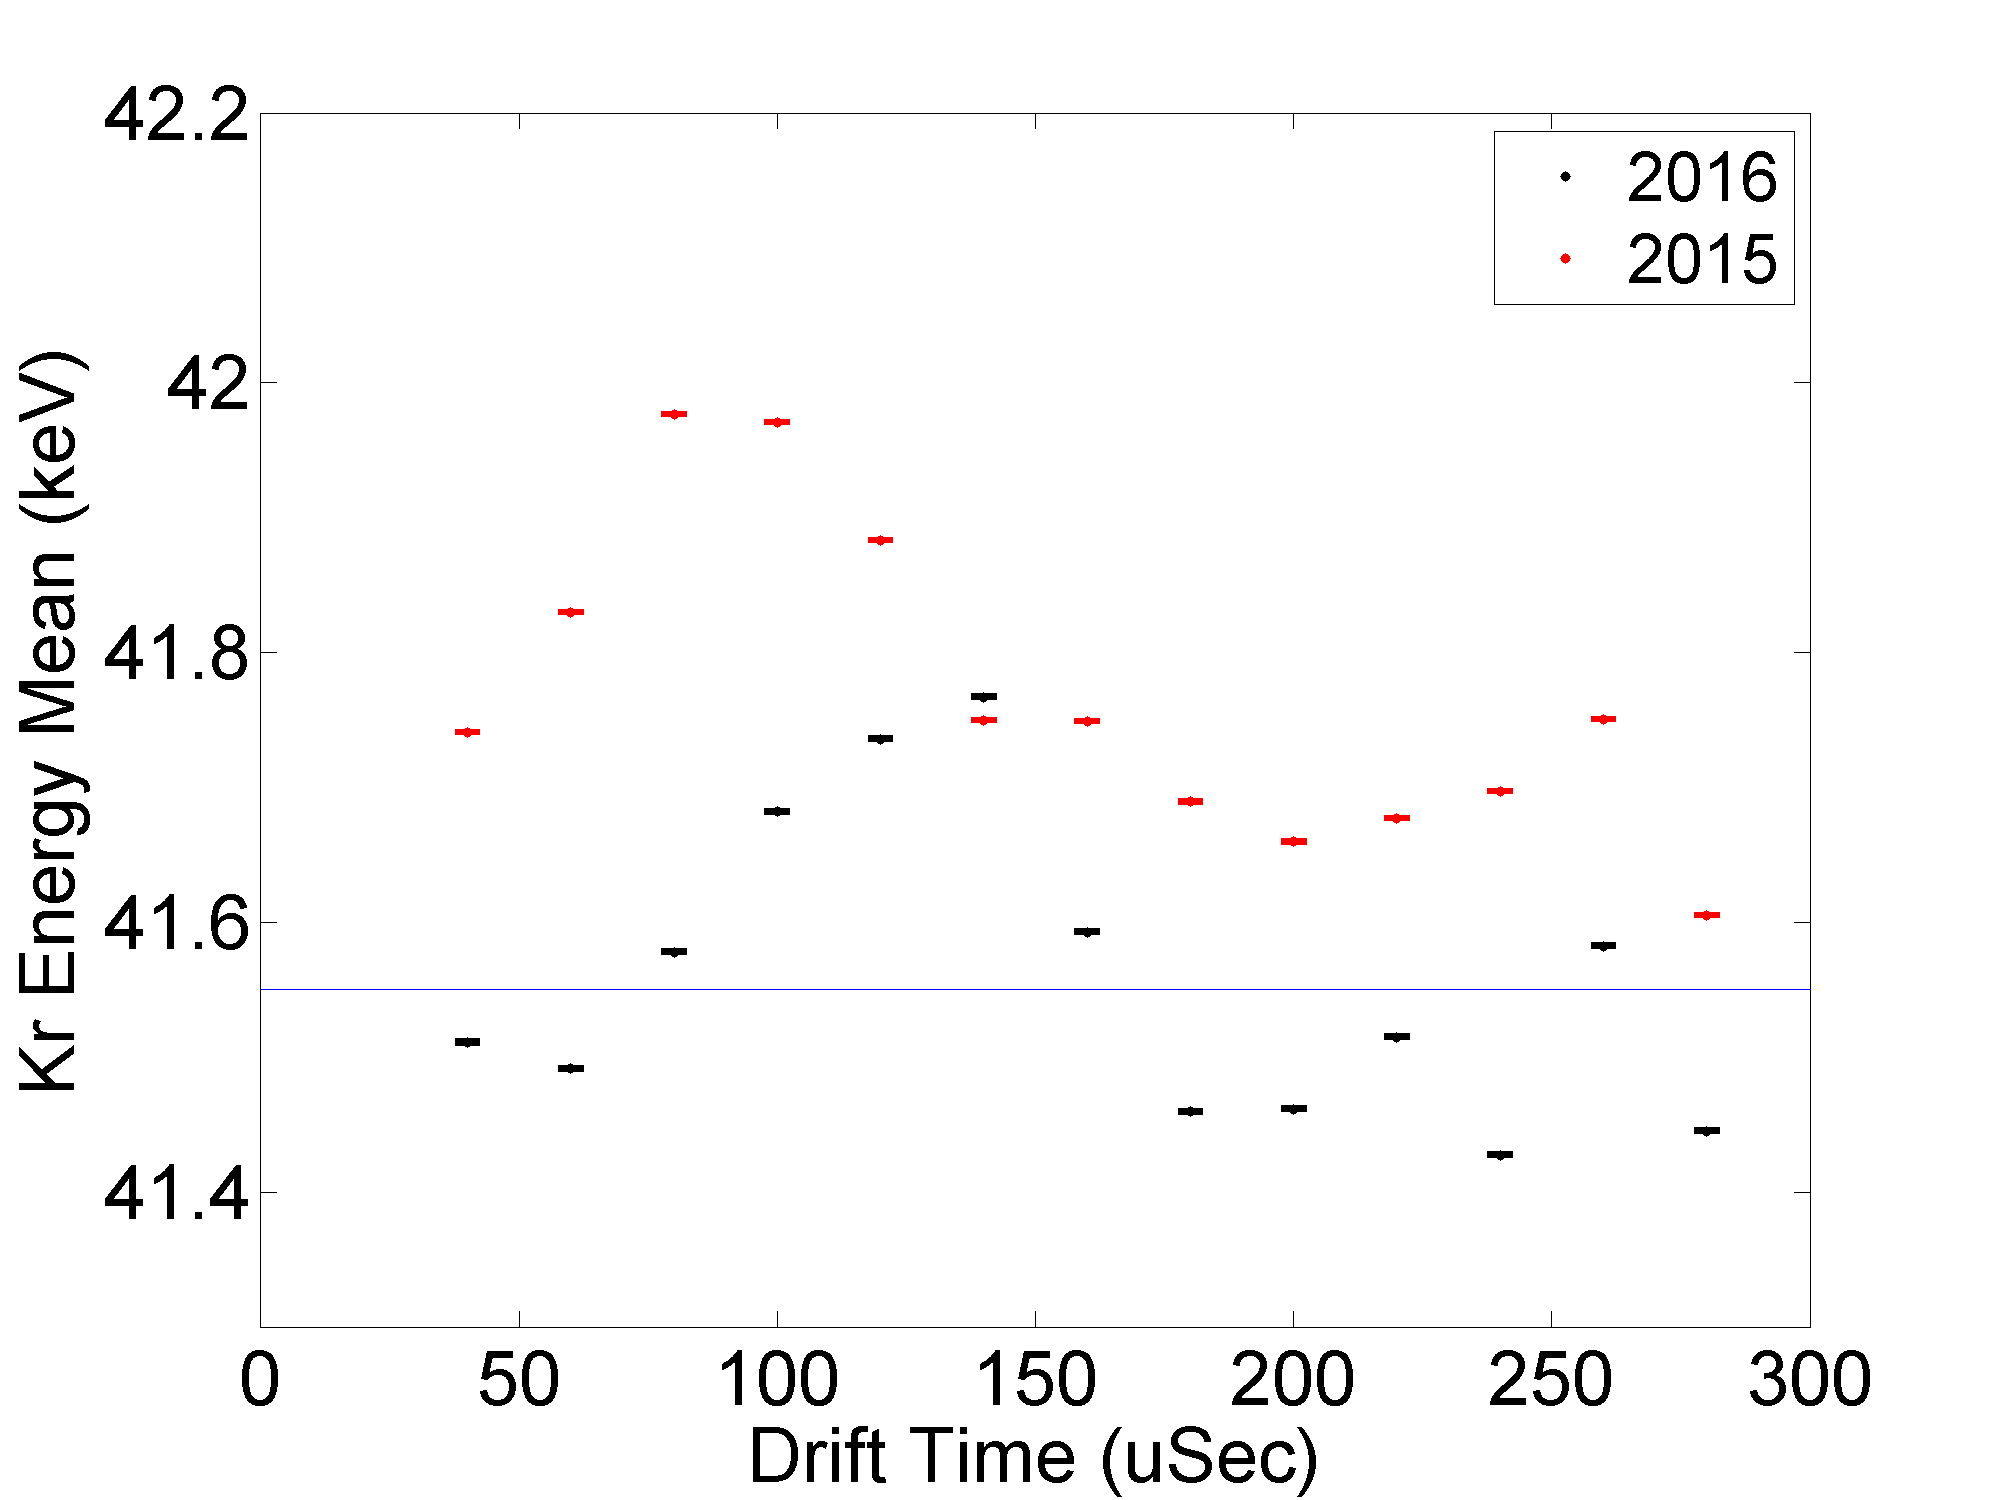
\includegraphics[width=6.5cm]{Run04Corrections/InferredS1Measure_KrSpectraZDep.png} }}
\captionof{figure}{ (Left) The energy spectrum of efficiency corrected  $^{83m}$Kr data in September 2015 (red) and February 2016(blue) after utilizing the S1 field effect measurements from this section in KrypCal. (Right) The Z dependence of the $^{83m}$Kr energy peaks in September 2015 (red) and February 2016 (black) and the expected energy (blue).}
\label{ShittyKr}
\end{figure}

\subsubsection{Measuring the S1a/S1b Ratio to S1 Field Effect Relationship with the S1a Signal} \label{MatthewsIdea}

The relative light yield of the $^{83m}$Kr 32.1 keV decay, $^{83m}$Kr 9.4 keV decay, and $^{57}$Co 122 keV decay has been measured as a function of the light yield at an applied electric field divided by the light yield at zero electric field by Manalaysay, et al. in reference \cite{Manalaysay}. (Figure \ref{FieldQuenching})  We can combine NEST predictions for the light yield of the 122 keV $^{57}$Co line with the ratio of the light yield of the 32.1 keV $^{83m}$Kr line to the 122 keV $^{57}$Co line from reference \cite{Manalaysay} to convert the relative light yield measurements to absolute light yield measurements.  This results in an empirical formula for the absolute light yield of the $^{83m}$Kr 32.1 keV decay as a function of electric field given by
\begin{equation}
\frac{\gamma}{E} = 55.2[1-0.0004895 \times F \times \ln{(1 + 1/(8.9\mathrm{e}{-4} \times F))}]
\label{S1aYield}
\end{equation}
where $\gamma$ is the number of photons, $E$ is the energy of the decay in keV, and $F$ is the applied electric field in units of V/cm.  

Using equation \ref{S1aYield} we can directly measure the strength of the field effect in the $^{83m}$Kr S1 data and relate it to the S1a/S1b ratio.  We begin by using the electric field to S1a/S1b relationships shown in Figure \ref{FieldToS1aS1b}, as well as the RvZ and three dimensional electric field maps to estimate the electric field in the detector in September 2015.  The average of the three electric field maps is taken as the measurement of the electric field, and the difference in each of the three electric field maps is taken as a systematic error.  The electric field map is converted to a map of the expected light yield at 32.1 keV using equation \ref{S1aYield}, assuming no detector inefficiency effects are present. The three dimensional spatial dependence of the light yield provides a direct measurement of the strength of the field effect in the S1a data, given by $\gamma(xyz)$/$\gamma(center)$.  Note that the strength of the field effect in the S1a data can help us derive the strength of the field effect in the combined S1 data, but the two are not equivalent.  Normalizing the field effect in the S1a data to the center of the detector, as shown in equation \ref{S1aNorm}, produces S1a$_F$ data which has spatial variation due to detector inefficiency effects only.  
\begin{equation}
S1a_F = S1a \frac{\gamma(center)}{\gamma(xyz)}
\label{S1aNorm}
\end{equation}
We measure the detector inefficiency effects in the S1a$_F$ data by dividing the detector into three dimensional voxels with X and Y width of 7 cm and Z width of 47 $\mu$s.  A Gaussian distribution is fit to the S1a$_F$ spectrum in each voxel, and the Gaussian mean is used to determine the spatial dependence of the S1a$_F$ data due to detector inefficiency effects alone.  Since the detector inefficiency effects are not dependent on the energy of an event, the spatial variation measured in the S1a$_F$ data is equivalent to the spatial variation in the combined S1 data due to detector inefficiency effects alone.  Therefore, we can use the spatial variation measured in the S1a$_F$ data to produce detector inefficiency corrected combined S1$_E$ data as shown in the equation
\begin{equation}
S1_E= S1 \frac{S1a_F(center)}{S1a_F(xyz)}.
\end{equation}
Any residual spatial variation in the detector inefficiency corrected combined S1$_E$ data is due to field effects in the combined $^{83m}$Kr S1 data alone.  We measure the strength of these field effects by again dividing the detector into three dimensional voxels with X and Y width of 7 cm and Z width of 47 $\mu$s.  A Gaussian distribution is fit to the S1$_E$ spectrum in each voxel, and the Gaussian mean is used to determine the spatial dependence of the S1a$_E$ data due to field effects alone.  At the same time, we use separate Gaussian distribution fits to the S1a and S1b data in each voxel to measure the spatial dependence of the S1a/S1b ratio.  Finally, we relate the S1a$_E$ Gaussian mean to the S1a/S1b ratio of each voxel and fit a second order polynomial which describes the strength of the field effect in the $^{83m}$Kr combined S1 signal to the data. (Figure \ref{S1aFieldEffect}) 


\begin{figure}[!h]
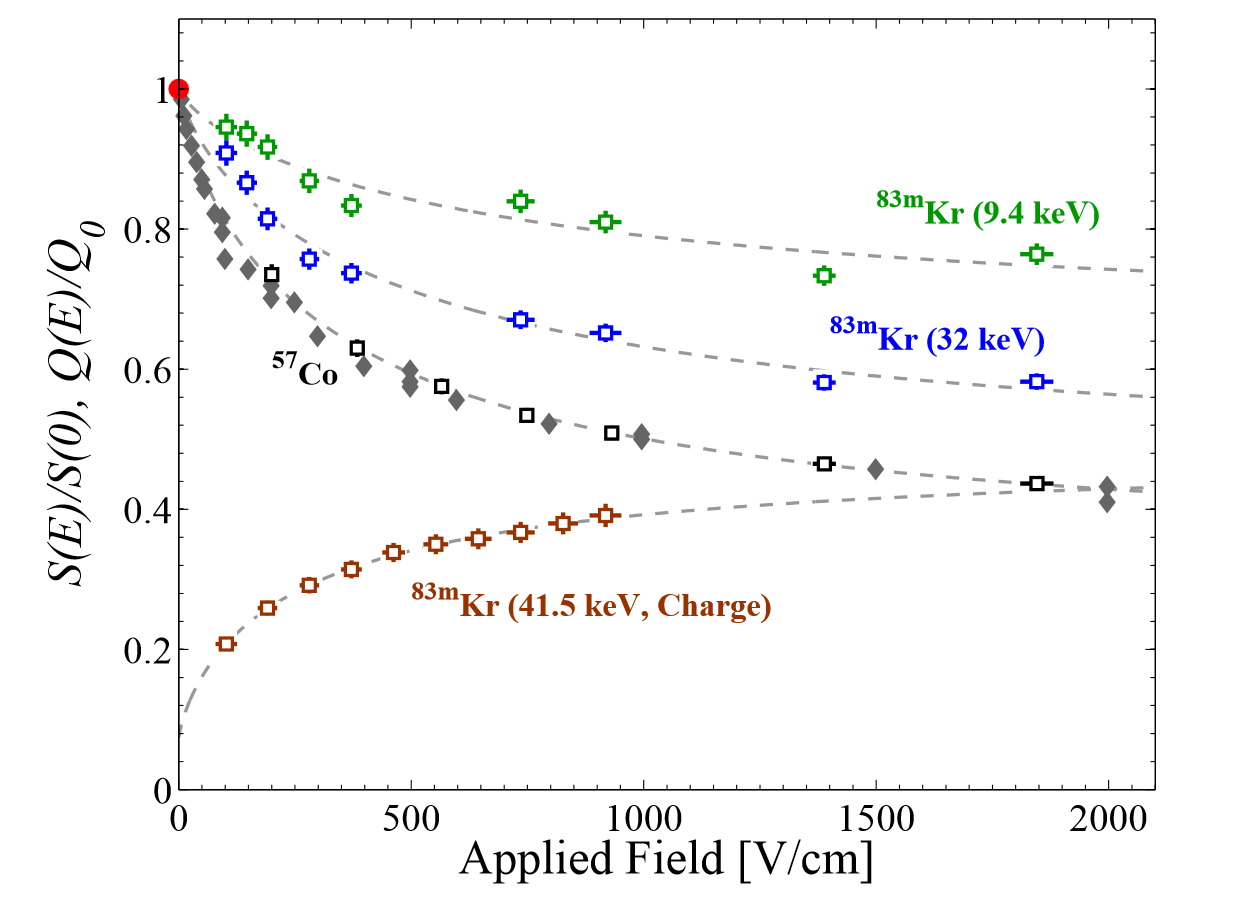
\includegraphics[scale=0.3]{Run04Corrections/ManalaysayFieldQuenching.png}
\captionof{figure}{Relative light yield of the $^{83m}$Kr and $^{57}$Co decays defined as the light yield at an applied field divided by the light yield at zero field.  Historical data for the $^{57}$Co relative light yield is shown by the grey diamond points.  Dashed lines correspond to fit parameters to the data.}
 \label{FieldQuenching}
\end{figure}

\begin{figure}[!h]
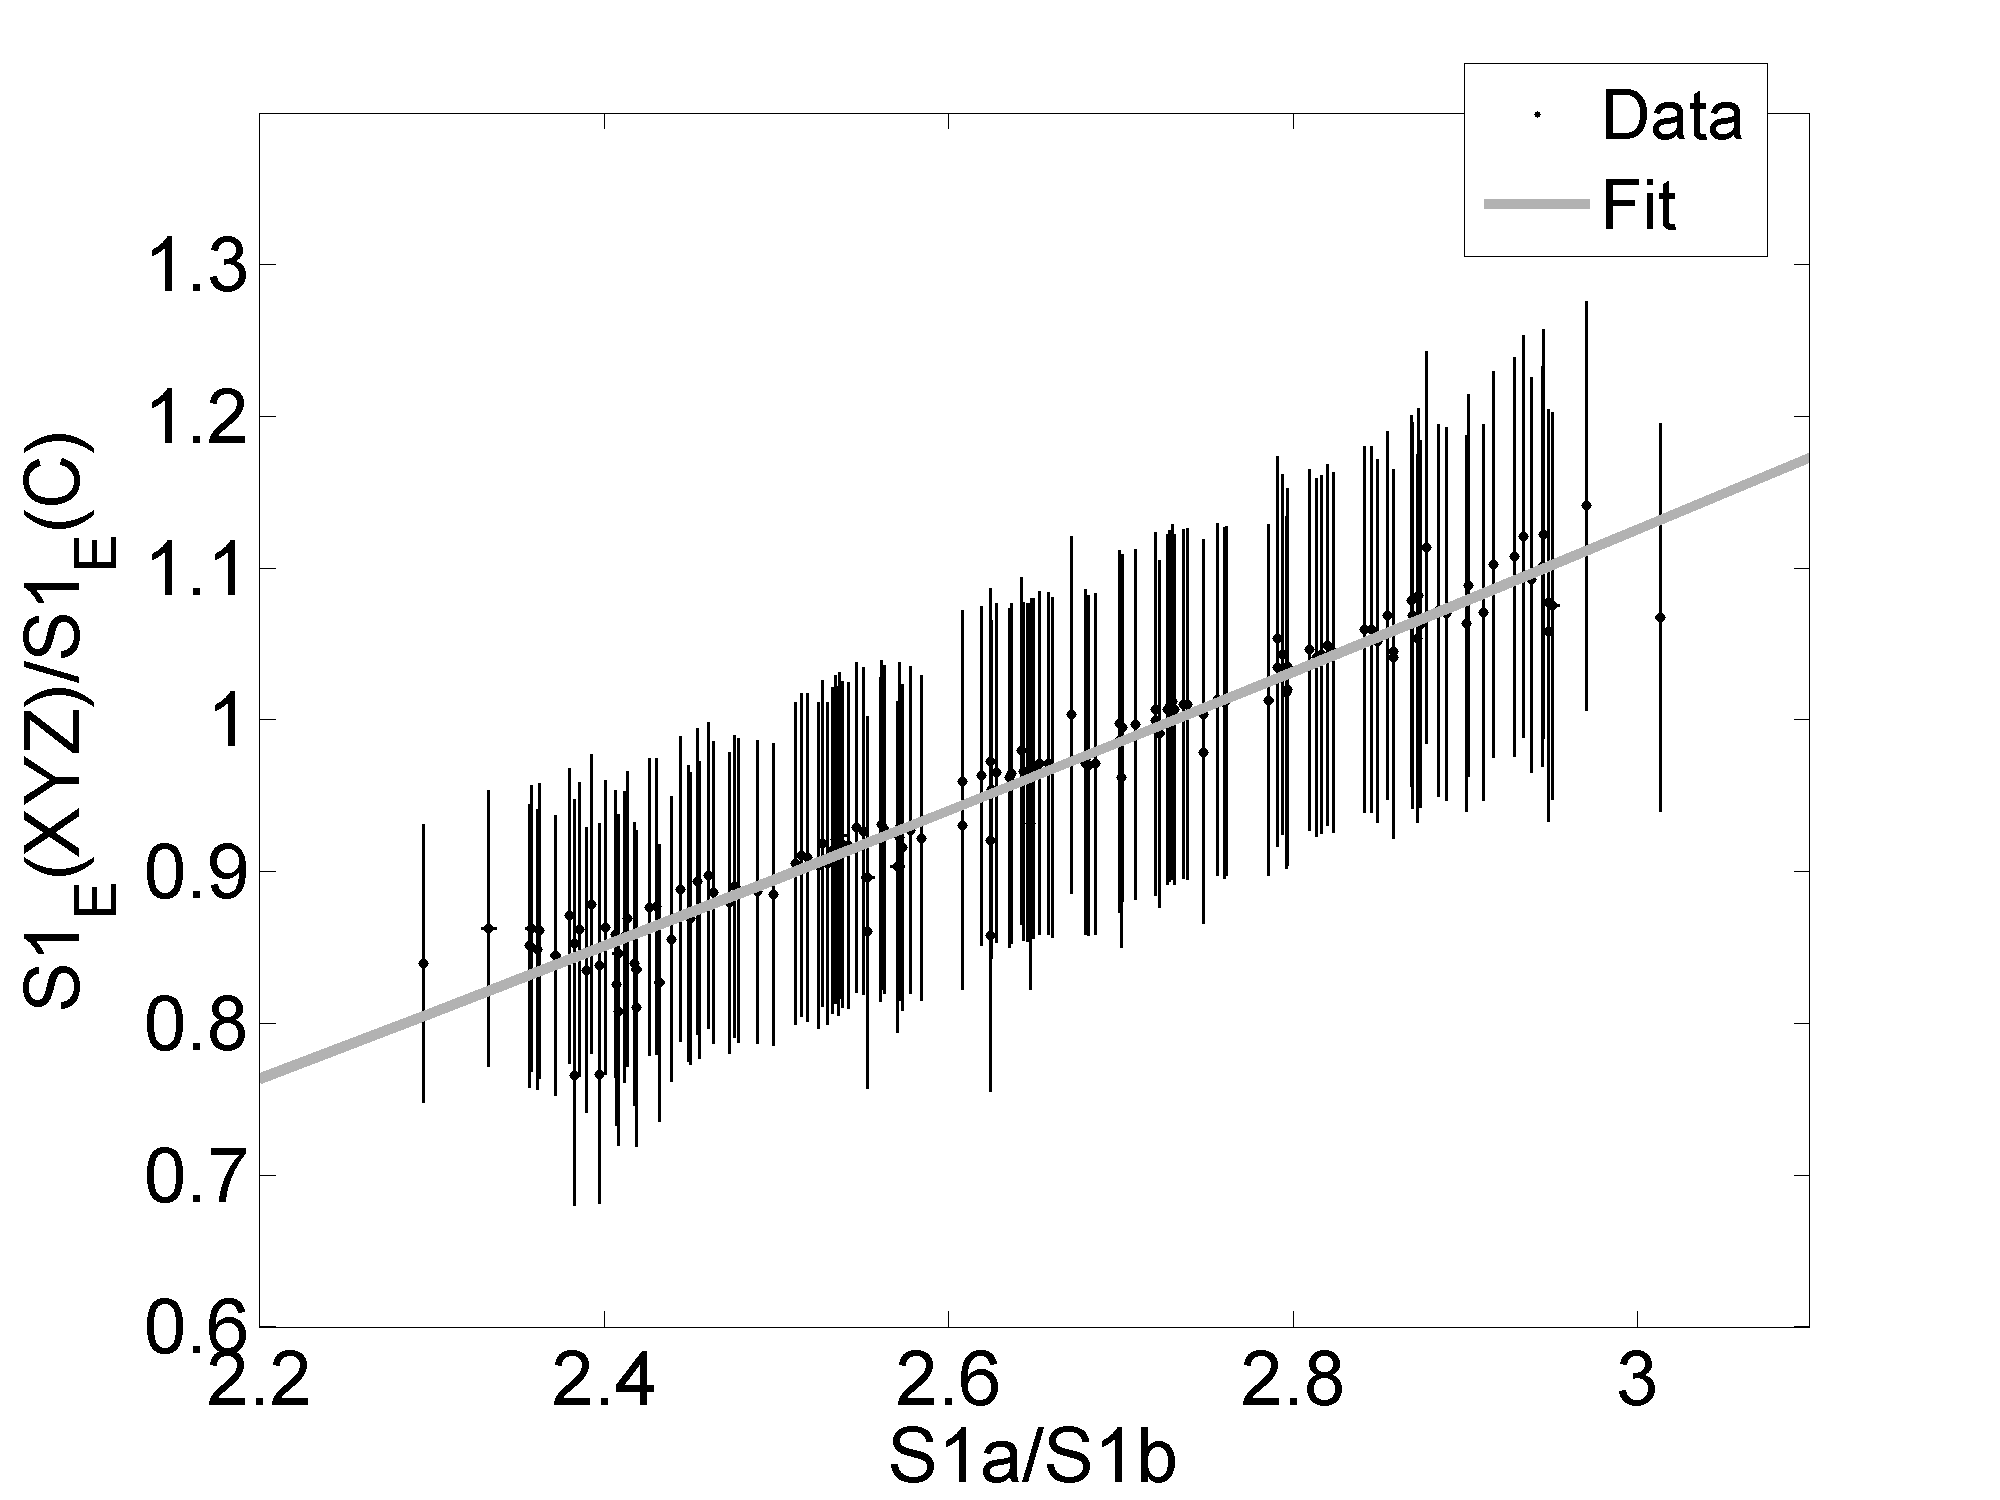
\includegraphics[scale=0.4]{Run04Corrections/MatthewS1FieldEffectMeasurement.png}
\captionof{figure}{The strength of the S1 field effect measured in this section (grey) compared to the strength of the S1 field effect measured in section \ref{section:S1relation2} (blue).  The large error bars on the data are due to systematic uncertainties in the field maps detector inefficiency corrections.}
\label{S1aFieldEffect}
\end{figure}

We can use the direct measurement of the S1a/S1b ratio to S1 field effect relationship measured in this section with the direct measurement of the S1a/S1b ratio to S2 field effect relationship measured in section \ref{section:S1aS1b2} to remove the field effects in $^{83m}$Kr data and produce detector inefficiency corrections via the methods in section \ref{KrypCalCode}.  The result of this is shown in Figure \ref{ShittyCH3T2} and Figure \ref{ShittyKr2}.  A $\chi^2$ fit to the expected CH$_3$T and $^{83m}$Kr energy spectra returns an average reduced $\chi^2$ of 2.22, with a reduced $\chi^2$ of 196/124=1.58 for CH$_3$T alone, and a reduced $\chi^2$ of 74.2/26=2.85 for $^{83m}$Kr alone using the best fit parameters of $g1=0.100$ and $EE=0.76$.  The large systematic errors in the S1a/S1b ratio to field effect relationships, introduced by uncertainties in the field maps and systematic errors in the detector inefficiency corrections, lead to unoptimized energy spectra when the two direct measurement results are combined.  Therefore, we turn to a $\chi^2$ minimization method in section \ref{section:S1relation2} to determine the optimal S1 field effect to S1a/S1b relationship and S2 field effect to S1a/S1b relationship.



\begin{figure} [!h]
\centering
\subfloat{{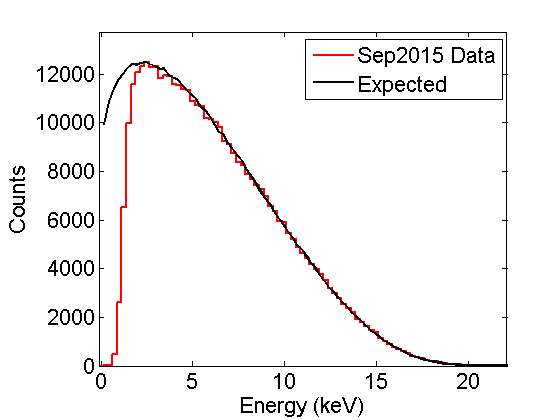
\includegraphics[width=6.5cm]{Run04Corrections/CH3T_Sep2015_Energy_BothDirectMeasured.png} }}
\qquad
\subfloat{{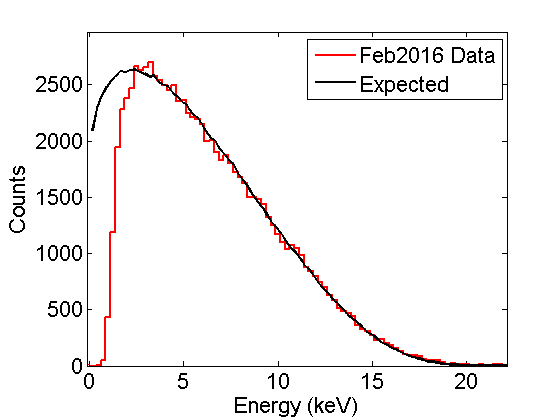
\includegraphics[width=6.5cm]{Run04Corrections/CH3T_Feb2016_Energy_BothDirectMeasured.png} }}
\captionof{figure}{The energy spectrum of the efficiency corrected  CH$_3$T data (red) after utilizing the S1 field effect measurements from this section and the S2 field effect measurements from section \ref{section:S1aS1b2} in September 2015 (left) and February 2016 (right). The expected energy spectrum is shown in black. }
\label{ShittyCH3T2}
\end{figure}

\begin{figure} [!h]
\centering
\subfloat{{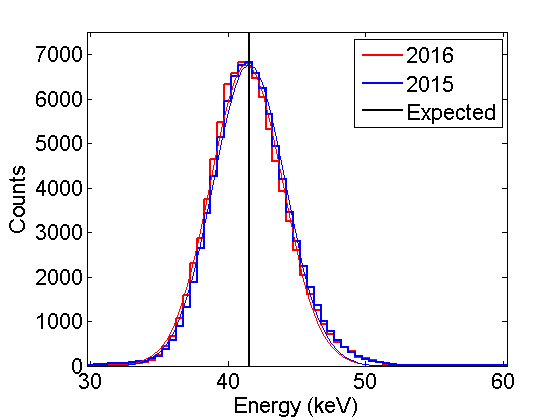
\includegraphics[width=6.5cm]{Run04Corrections/KrEnergy_BothDirectMeasured.png} }}
\qquad
\subfloat{{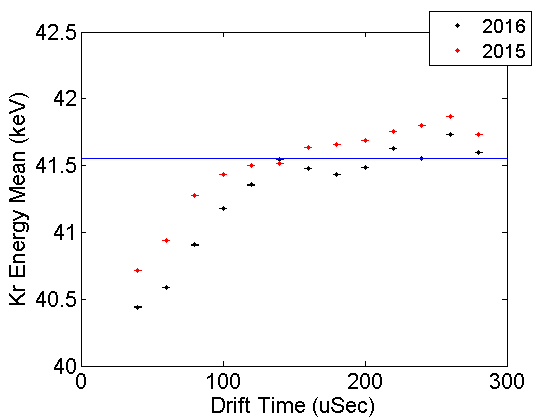
\includegraphics[width=6.5cm]{Run04Corrections/KrEnergyZDep_BothDirectMeasured.png} }}
\captionof{figure}{ (Left) The energy spectrum of efficiency corrected  $^{83m}$Kr data in February 2016 (red) and September 2015(blue) after utilizing the S1 field effect measurements from this section and the S2 field effect measurements from section \ref{section:S1aS1b2} in KrypCal. (Right) The Z dependence of the $^{83m}$Kr energy peaks in September 2015 (red) and February 2016 (black).}
\label{ShittyKr2}
\end{figure}


\subsubsection{Expectation for G1}\label{G1pred}

The process described in section \ref{MatthewsIdea} also yields an expectation for the value of $g_1$ in Run4.  First, we measure the mean of the S1a distribution at the center.  This is equivalent to measuring the inefficiency corrected S1a$_E$ data given by 
\begin{equation}
S1a_E=S1a \frac{S1a_F(center)}{S1a_F(xyz)}
\end{equation}
since we normalize the detector inefficiency effects to the center of the detector.  Combining this measurement with equation \ref{S1aYield}, which predicts the number of photons produced by a 32.1 keV decay at the center of the detector, provides a prediction for the gain factor $g_1$ given by
\begin{equation}
g_1 = \frac{S1a(center)}{\gamma (center)}.
\end{equation}
The result of this prediction is g$_1$=0.108 $\pm$ 0.010, where systematic errors from the field map measurement and the parameters in equation  \ref{S1aYield} have been included in the result.  Note that this prediction is only one sigma below the optimal value of $g_1$ found in the following section, showing consistency between the two measurements.

\subsubsection{Measuring the S1a/S1b Ratio to S1 Field Effect Relationship with $\chi^2$ Fitting Methods} \label{section:S1relation2}

Although field induced variation in the recombination of a $^{83m}$Kr event can introduce a spatial and time dependence in the $^{83m}$Kr S1 and S2 signals, the total energy signal given (with gain factors $g_1$ and $g_2$, and a $W$ value of 1/73) by 
\begin{equation} \label{CombinedEnergy}
E=\left(\frac{1}{73}\right)\left(\frac{S1_E}{g_1} + \frac{S2_E}{g_2}\right)
\end{equation}
should be insensitive to field variations.  We can take advantage of this fact to determine the optimal S1a/S1b to S1 field effect relationship corresponding to the directly measured S1a/S1b to S2 field effect relationship measured in section \ref{section:S1aS1b2}.  Since we desire an independent measurement of the S1 field effect, we do not want to rely on the S1 field effect measurement from section~\ref{MatthewsIdea} here.  Instead, we assume we do not have knowledge of the strength of the field effect in the $^{83m}$Kr S1 signal, so we can not remove the field effect from the data to produce the efficiency-only corrected S1$_E$ signal.  Likewise, without efficiency corrected data we can not measure the gain factors $g_1$ and $g_2$ to produce a combined energy spectrum.  The only tools that we have at our disposal are a measurement of the strength of the field effect in the $^{83m}$Kr S2 signal and its relationship to S1a/S1b, as well as the ability to produce efficiency only corrected $^{83m}$Kr S2$_E$ data based on to the spatial variation of field effect corrected  $^{83m}$Kr S2$_F$ data.  In this section we turn to a $\chi^2$ minimization approach which will float the S1 field effect to S1a/S1b relationship, produce inefficiency corrections based on the field removed S1$_F$ and S2$_F$ signals, and then float the gain factors $g_1$ and $g_2$ to produce an optimized combined energy spectrum.  

We begin by eliminating one of the three parameters associated with the second order polynomial which describes the S1 field effect to S1a/S1b relationship.  We choose to normalize the spatial variation induced by the nonuniform electric field to the center of the detector, so the strength of the field effect as measured by $\frac{S1_{E,Kr}(xyz)}{S1_{E,Kr}(center)}$ must equal one at the center of the detector.  Therefore, we can relate one of the coefficients ($a$,$b$, and $c$) in the second order polynomial
\begin{equation}
 \frac{S1_{E,Kr}(xyz)}{S1_{E,Kr}(center)} = a\left(\frac{S1a}{S1b}\right)^2 + b\left(\frac{S1a}{S1b} \right) + c
 \end{equation}
 to the other two, such that
 \begin{equation}
 c=1-a\left(\frac{S1a_c}{S1b_c}\right)^2-b\left(\frac{S1a_c}{S1b_c}\right)
 \end{equation}
 where $S1a_c$ and $S1b_c$ represent the values of $S1a$ and $S1b$ at the center of the detector.  Next, we scan over a range of $a$ and $b$ values and produce the $\frac{S1_{E,Kr}(xyz)}{S1_{E,Kr}(center)}$ to $\frac{S1a}{S1b}$ relationship for each pair of $a$ and $b$ values.  We follow the procedure described in section \ref{KrypCalCode} and use the S1 field effect to S1a/S1b relationship from each pair of $a$ and $b$ values, in conjunction with the S2 field effect S1a/S1b relationship measured in \ref{section:FieldEffects}, to produce efficiency-only corrections for CH$_3$T data and $^{83m}$Kr data from September 2015 and February 2016. These corrections are used to produce S2$_E$ and S1$_E$ data for all four data sets.  We then scan over a range of $g_1$ and extraction efficiency (EE) values and use the S2$_E$ and S1$_E$ data to produce a combined energy spectrum (for each source) for each combination of $a$,$b$,$g_1$, and EE based on equation \ref{CombinedEnergy}.  Note that $g_2=SE \times EE$, where $SE$ is the single electron size at the time of each data set.  

To evaluate the performance of each $a$,$b$,$g_1$, and $EE$ combination we must develop models for the expected energy spectra of CH$_3$T and $^{83m}$Kr data in September 2015 and February 2016.  The $^{83m}$Kr events consist of a mono-energetic 32.1 keV decay and a mono-energetic 9.4 keV decay.  The expected energy spectrum is a Gaussian distribution centered around the sum of these two mono-energetic decays at 41.55 keV.  The width of the Gaussian distribution depends on a number of factors, including the detector's efficiency for collecting S1 and S2 light, as well as the spatial dependence of the recombination of $^{83m}$Kr events induced by the nonuniform electric field.  While we can measure most of these parameters, we would have to feed them into NEST to determine the final width of the Gaussian distribution.  Since NEST does not simulate $^{83m}$Kr events well, we can only use the mean of the Gaussian distribution as a figure of merit for the $^{83m}$Kr energy spectrum.

Tritium beta decays with an energy spectrum that has a broad peak at 2.5 keV and a smoothly falling distribution out to 18 keV.  As with $^{83m}$Kr, this spectrum is smeared based on a number of parameters.  Unlike $^{83m}$Kr, the smearing in CH$_3$T data can be accurately determined by NEST so we can compare the energy spectrum from data to simulations on a bin by bin basis. 

For each $a$,$b$,$g_1$, and $EE$ combination a reduced $\chi^2$ for the CH$_3$T and $^{83m}$Kr data is measured using the difference between the expected energy spectra and measured energy spectra.   During the $^{83m}$Kr $\chi^2$ calculation, the energy spectrum is from each point in time is divided into drift time bins so that the spatial dependence of the energy spectrum is included in the $\chi^2$ measurement.  The $^{83m}$Kr data has very high statistics, and only the mean of a Gaussian fit to the data is of interest, so the variance used in the $\chi^2$  measurement  is dominated by systematic error.  We use the standard deviation of the $^{83m}$Kr energy spectrum over the duration of Run3 to evaluate the size of this systematic error, and find $\sigma = 0.2395$ keV.  During the CH$_3$T $\chi^2$  calculation, the energy spectrum is divided into energy bins so that the entire beta spectrum (above 3.5 keV to avoid the detector threshold) is included in the $\chi^2$ measurement.  The variance of the CH$_3$T data is based on statistics alone, due to finer binning and lower statistics of the data.  We choose to define a total reduced $\chi^2$ (to be minimized in the $\chi^2$ fit) as the average of the reduced $\chi^2$ for the $^{83m}$Kr and CH$_3$T data, so that each source carries the same amount of weight in the fit. A minimum average reduced  $\chi^2$ of 0.8413 is found for the best fit parameters of $a=0.065 \pm 0.0117$,$b=0.020 \pm 0.060$,$g_1=0.0980 \pm 0.001$, and $EE=0.808 \pm 0.029$. The corresponding value of the zeroth order coefficient is $c=0.461 \pm 0.186$.  The reduced $\chi^2$ of the $^{83m}$Kr and CH$_3$T energy spectra separately are 12.17/26=0.4682 (p=0.99) and 150.6/124=1.2143 (p=0.05), respectively. Note that (as we will see in section \ref{Results}) the extraction efficiency needed to produce these results is consistent with our expectations, and the results produce $^{83m}$Kr energy peaks (unbinned in drift time) that are within one sigma of the expected 41.55 keV in both September 2015 and February 2016. 


\begin{figure} [!h]
\centering
\subfloat{{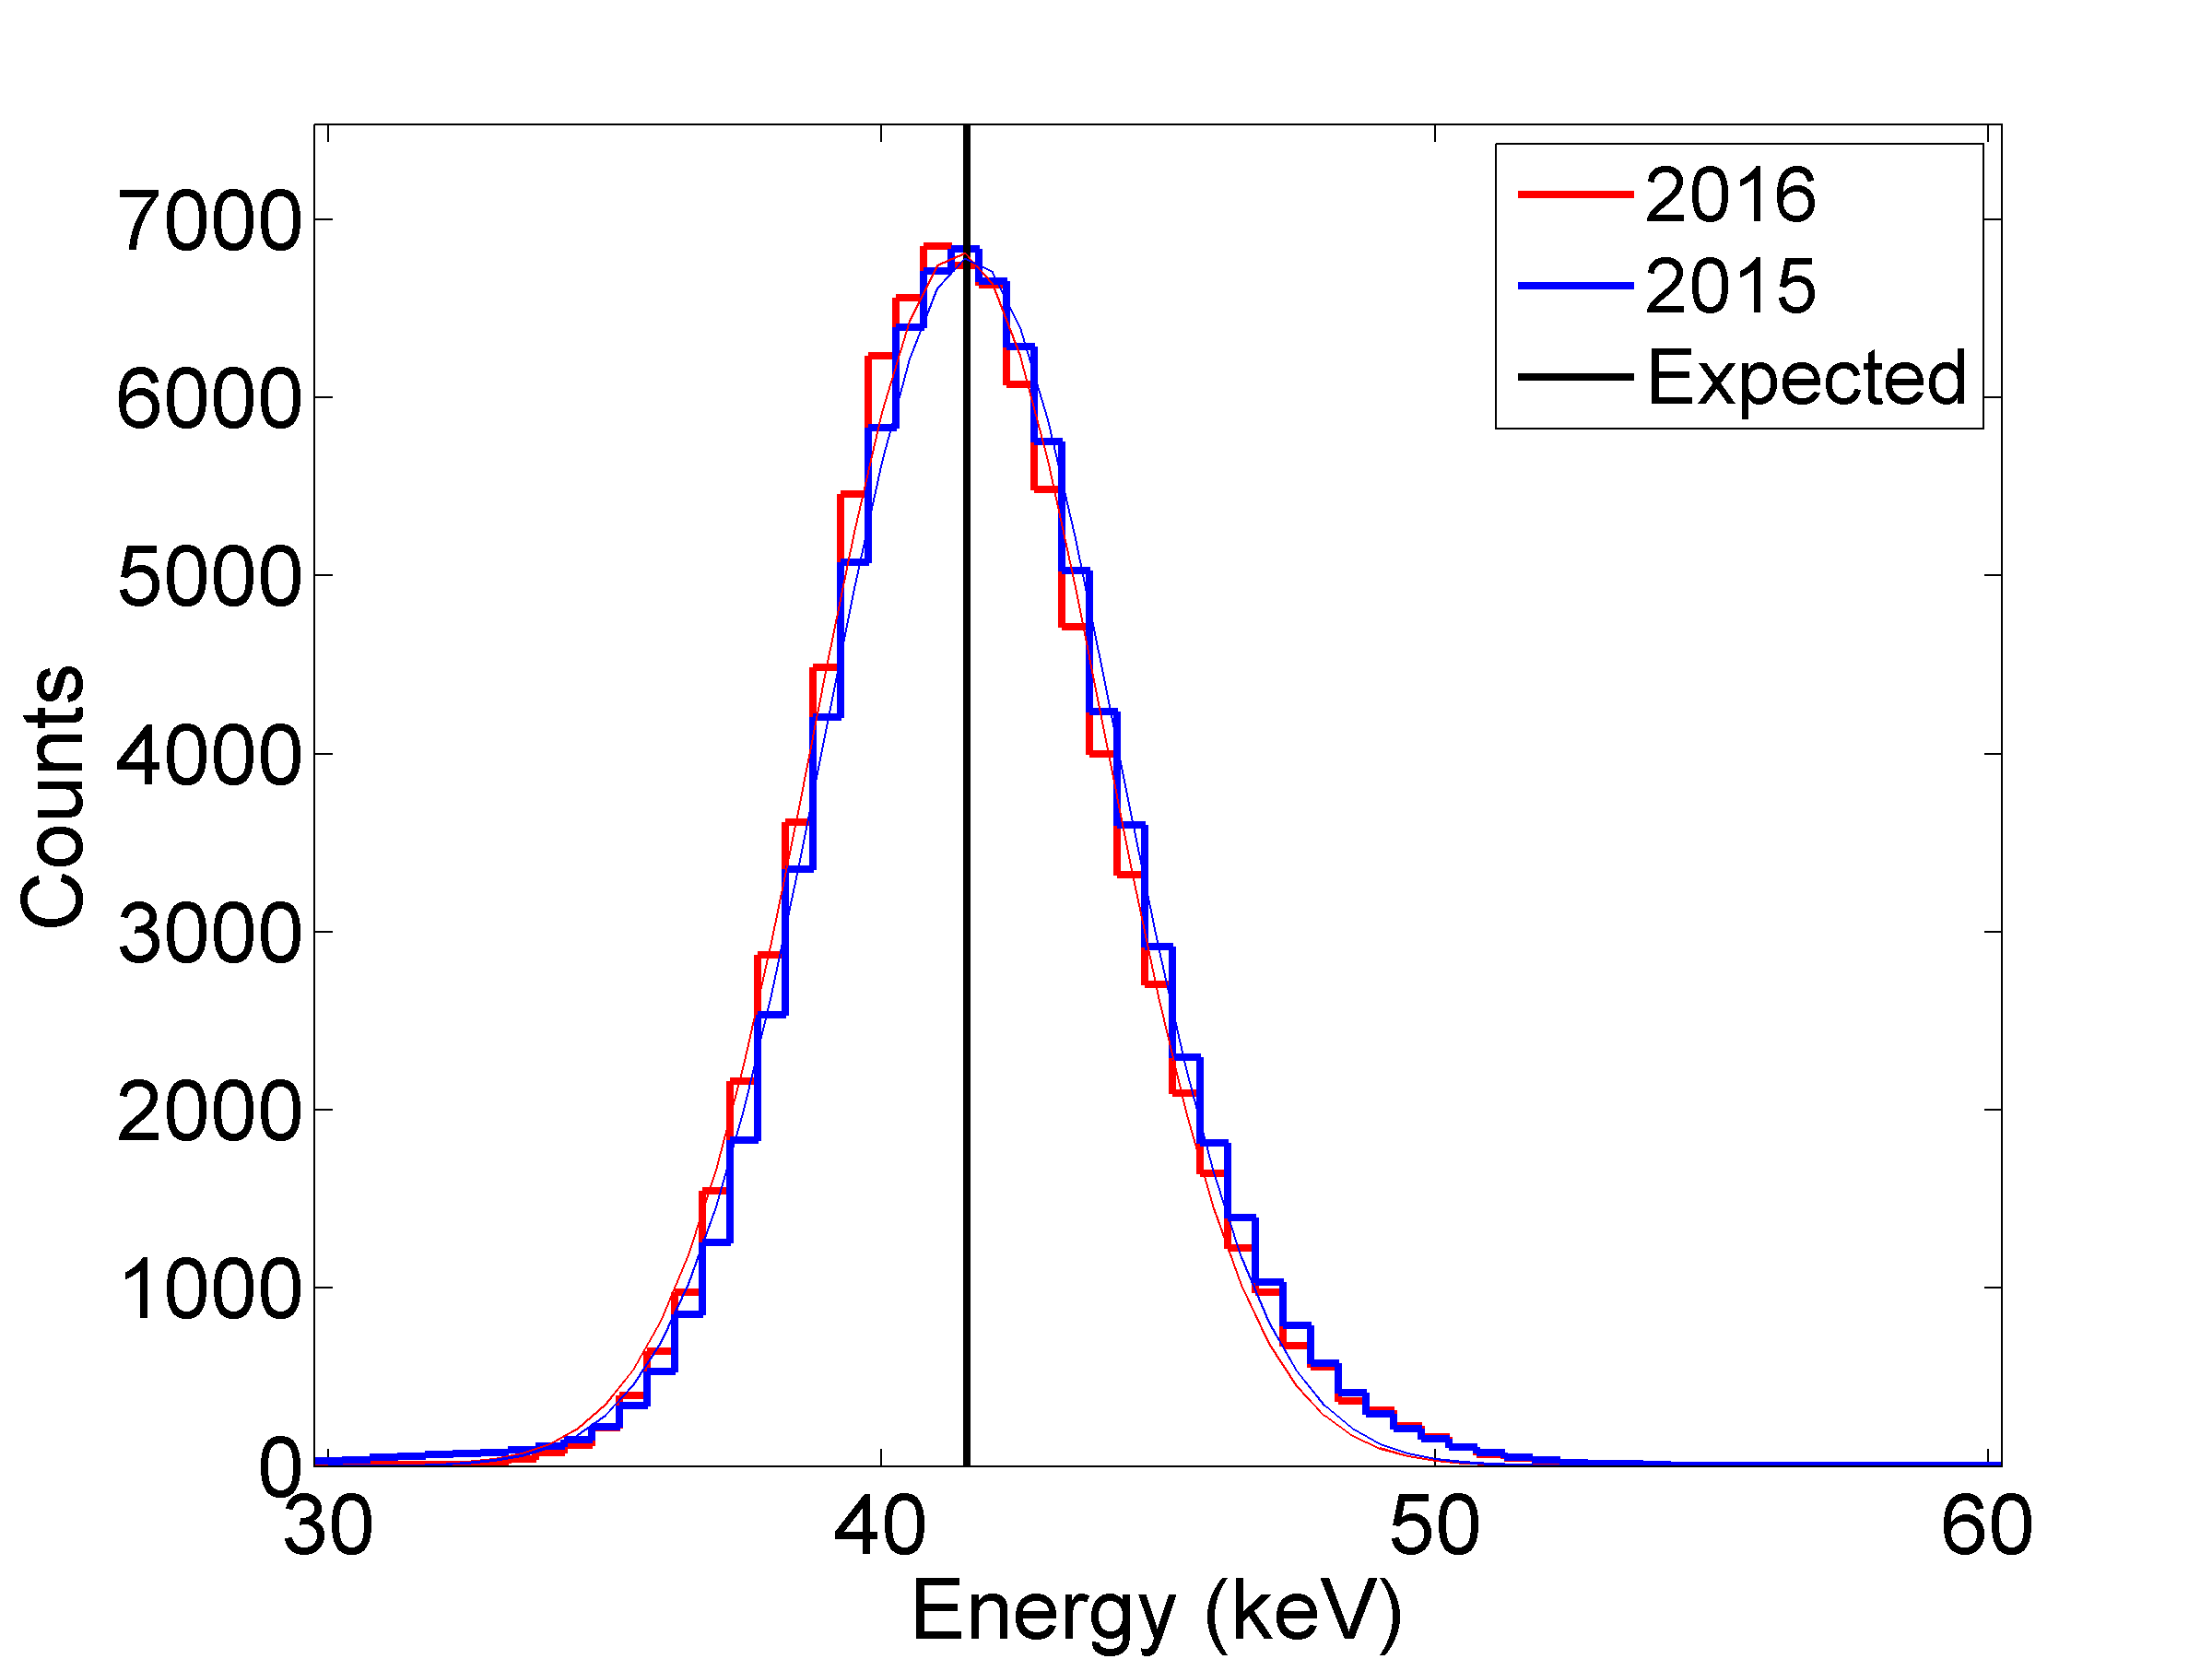
\includegraphics[width=6.5cm]{Run04Corrections/KrEnergy.png} }}
\qquad
\subfloat{{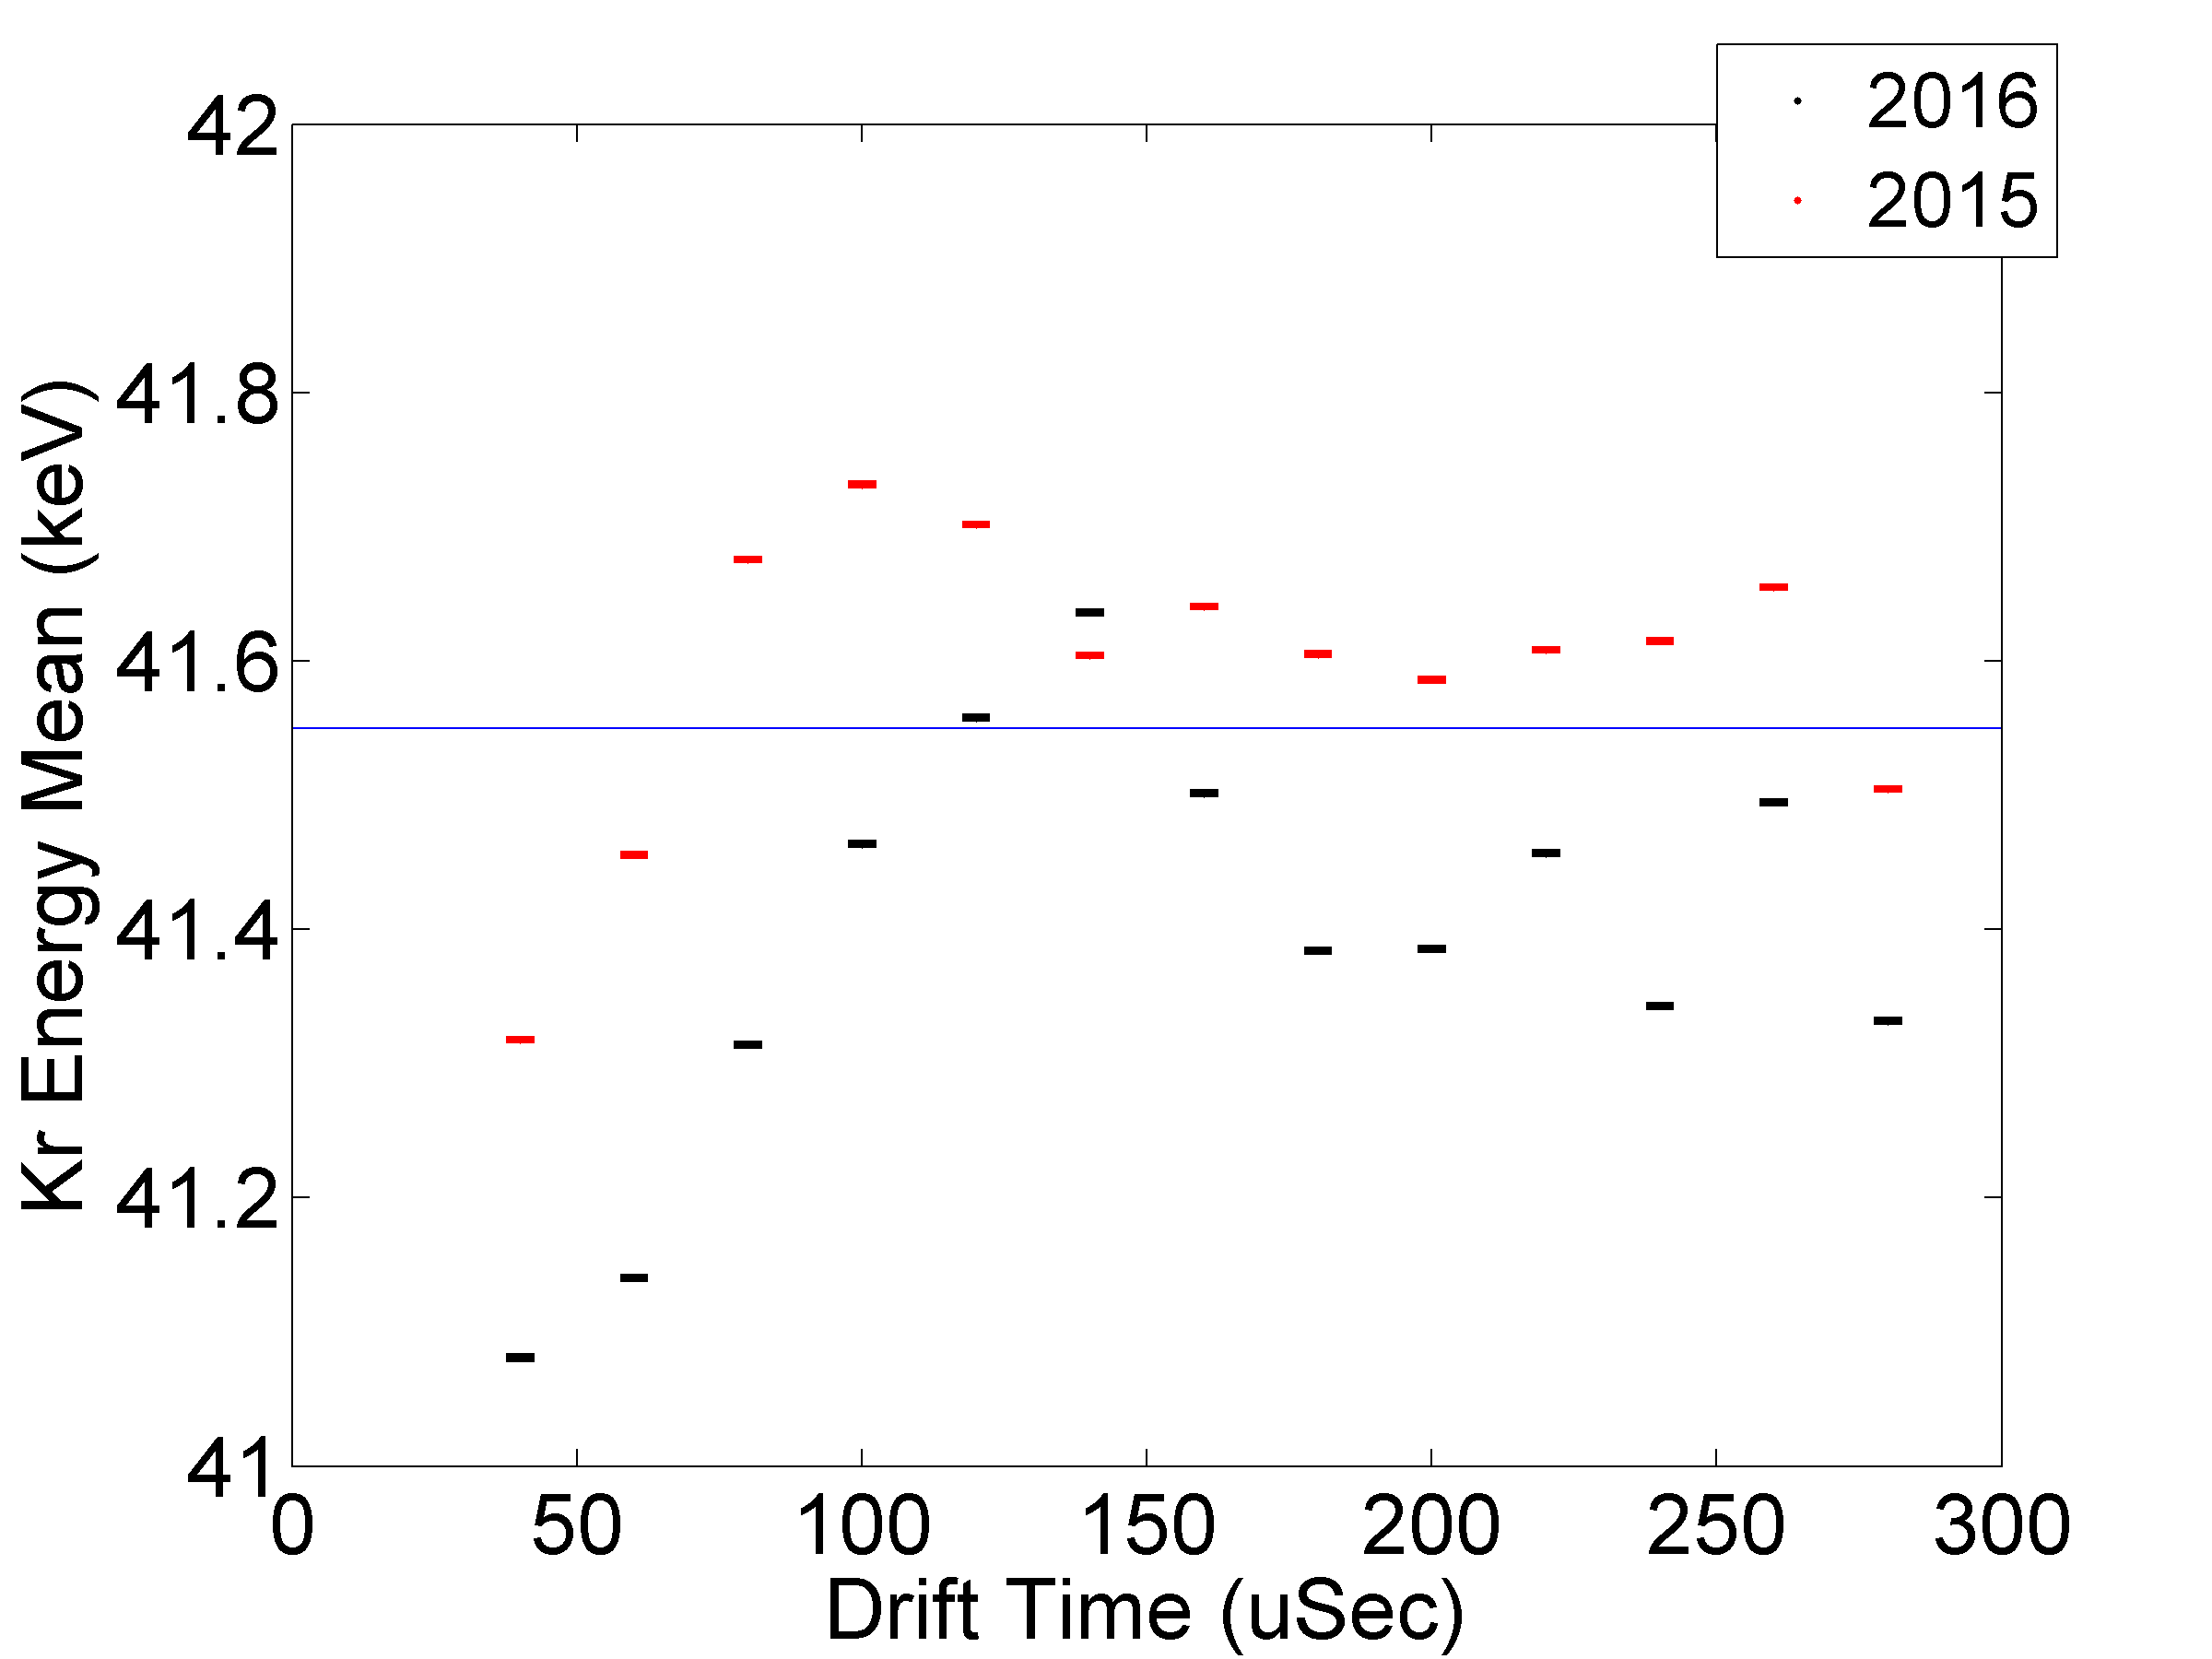
\includegraphics[width=6.5cm]{Run04Corrections/KrEnergyZDep.png} }}
\captionof{figure}{ (Left) The energy spectrum of $^{83m}$Kr data in February 2016 (red) and September 2015(blue) after determining the S1 field effect to S1a/S1b relationship from the reduced $\chi^2$ method. The energy spectrum is expected to be a Gaussian distribution centered around the black line.  (Right) The Z dependence of the $^{83m}$Kr energy peaks in September 2015 (red) and February 2016 (black).}
\label{Kr2p20}
\end{figure}



\begin{figure} [!h]
\centering
\subfloat{{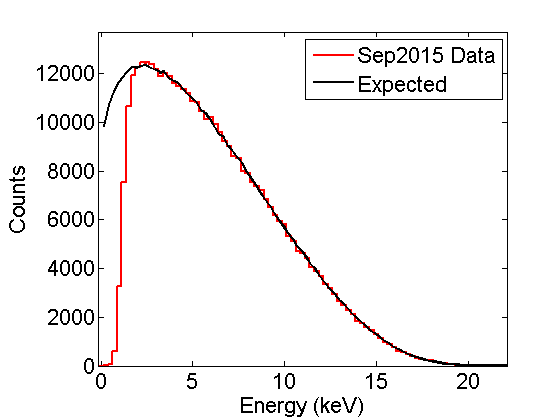
\includegraphics[width=6.5cm]{Run04Corrections/CH3T_Sep2015_Energy.png} }}
\qquad
\subfloat{{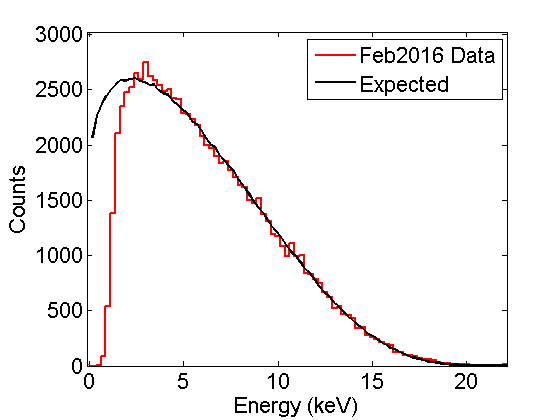
\includegraphics[width=6.5cm]{Run04Corrections/CH3T_Feb2016_Energy.png} }}
\captionof{figure}{ (Left) The energy spectrum of CH$_3$T data in September 2015 (left) and February 2016 (right) after determining the S1 field effect to S1a/S1b relationship from the reduced $\chi^2$ method.  The expected CH$_3$T energy spectrum for each data set is shown in black.}
\label{Kr2p20}
\end{figure}



\subsubsection{Summary of S1a/S1b Ratio to Field Effect Measurements}

We have directly measured the strength of the field effect in $^{83m}$Kr S2 data by removing detector inefficiency effects from the data with the help of CH$_3$T data.  We have also directly measured the strength of the field effect in $^{83m}$Kr S1 data using the expected light yield of the $^{83m}$Kr S1 data 32.1 keV decay.  Combining these two direct measurement techniques does not produce satisfactory energy spectra.  Instead, we turn to $\chi^2$ optimization methods to find the optimal S1 field effect to S1a/S1b relationship to pair with the direct S2 field effect measurement.  We find that the optimal S1 field effect found by a $\chi^2$ optimization agrees very closely with our expectations from recombination physics.  This promising result is bolstered by the improvements in the corrected data discussed in section \ref{Results}. We choose to use the S2 field relationship measured in section \ref{section:S1aS1b2} and the corresponding optimal S1 field effect relationship measured in section \ref{section:S1relation2} for our KrypCal work. The polynomials that describe these relationships are:
\begin{equation}
\frac{S2_{E,Kr}(xyz)}{S2_{E,Kr}(center)} =    -0.499 \left(\frac{S1a}{S1b} \right)^2 + 1.48  \left(\frac{S1a}{S1b} \right) + 0.667
\end{equation}
\begin{equation}
\frac{S1_{E,Kr}(xyz)}{S1_{E,Kr}(center)} =   0.065 \left(\frac{S1a}{S1b} \right)^2 + 0.020 \left(\frac{S1a}{S1b} \right) + 0.461
\end{equation}


\begin{figure}[!h]
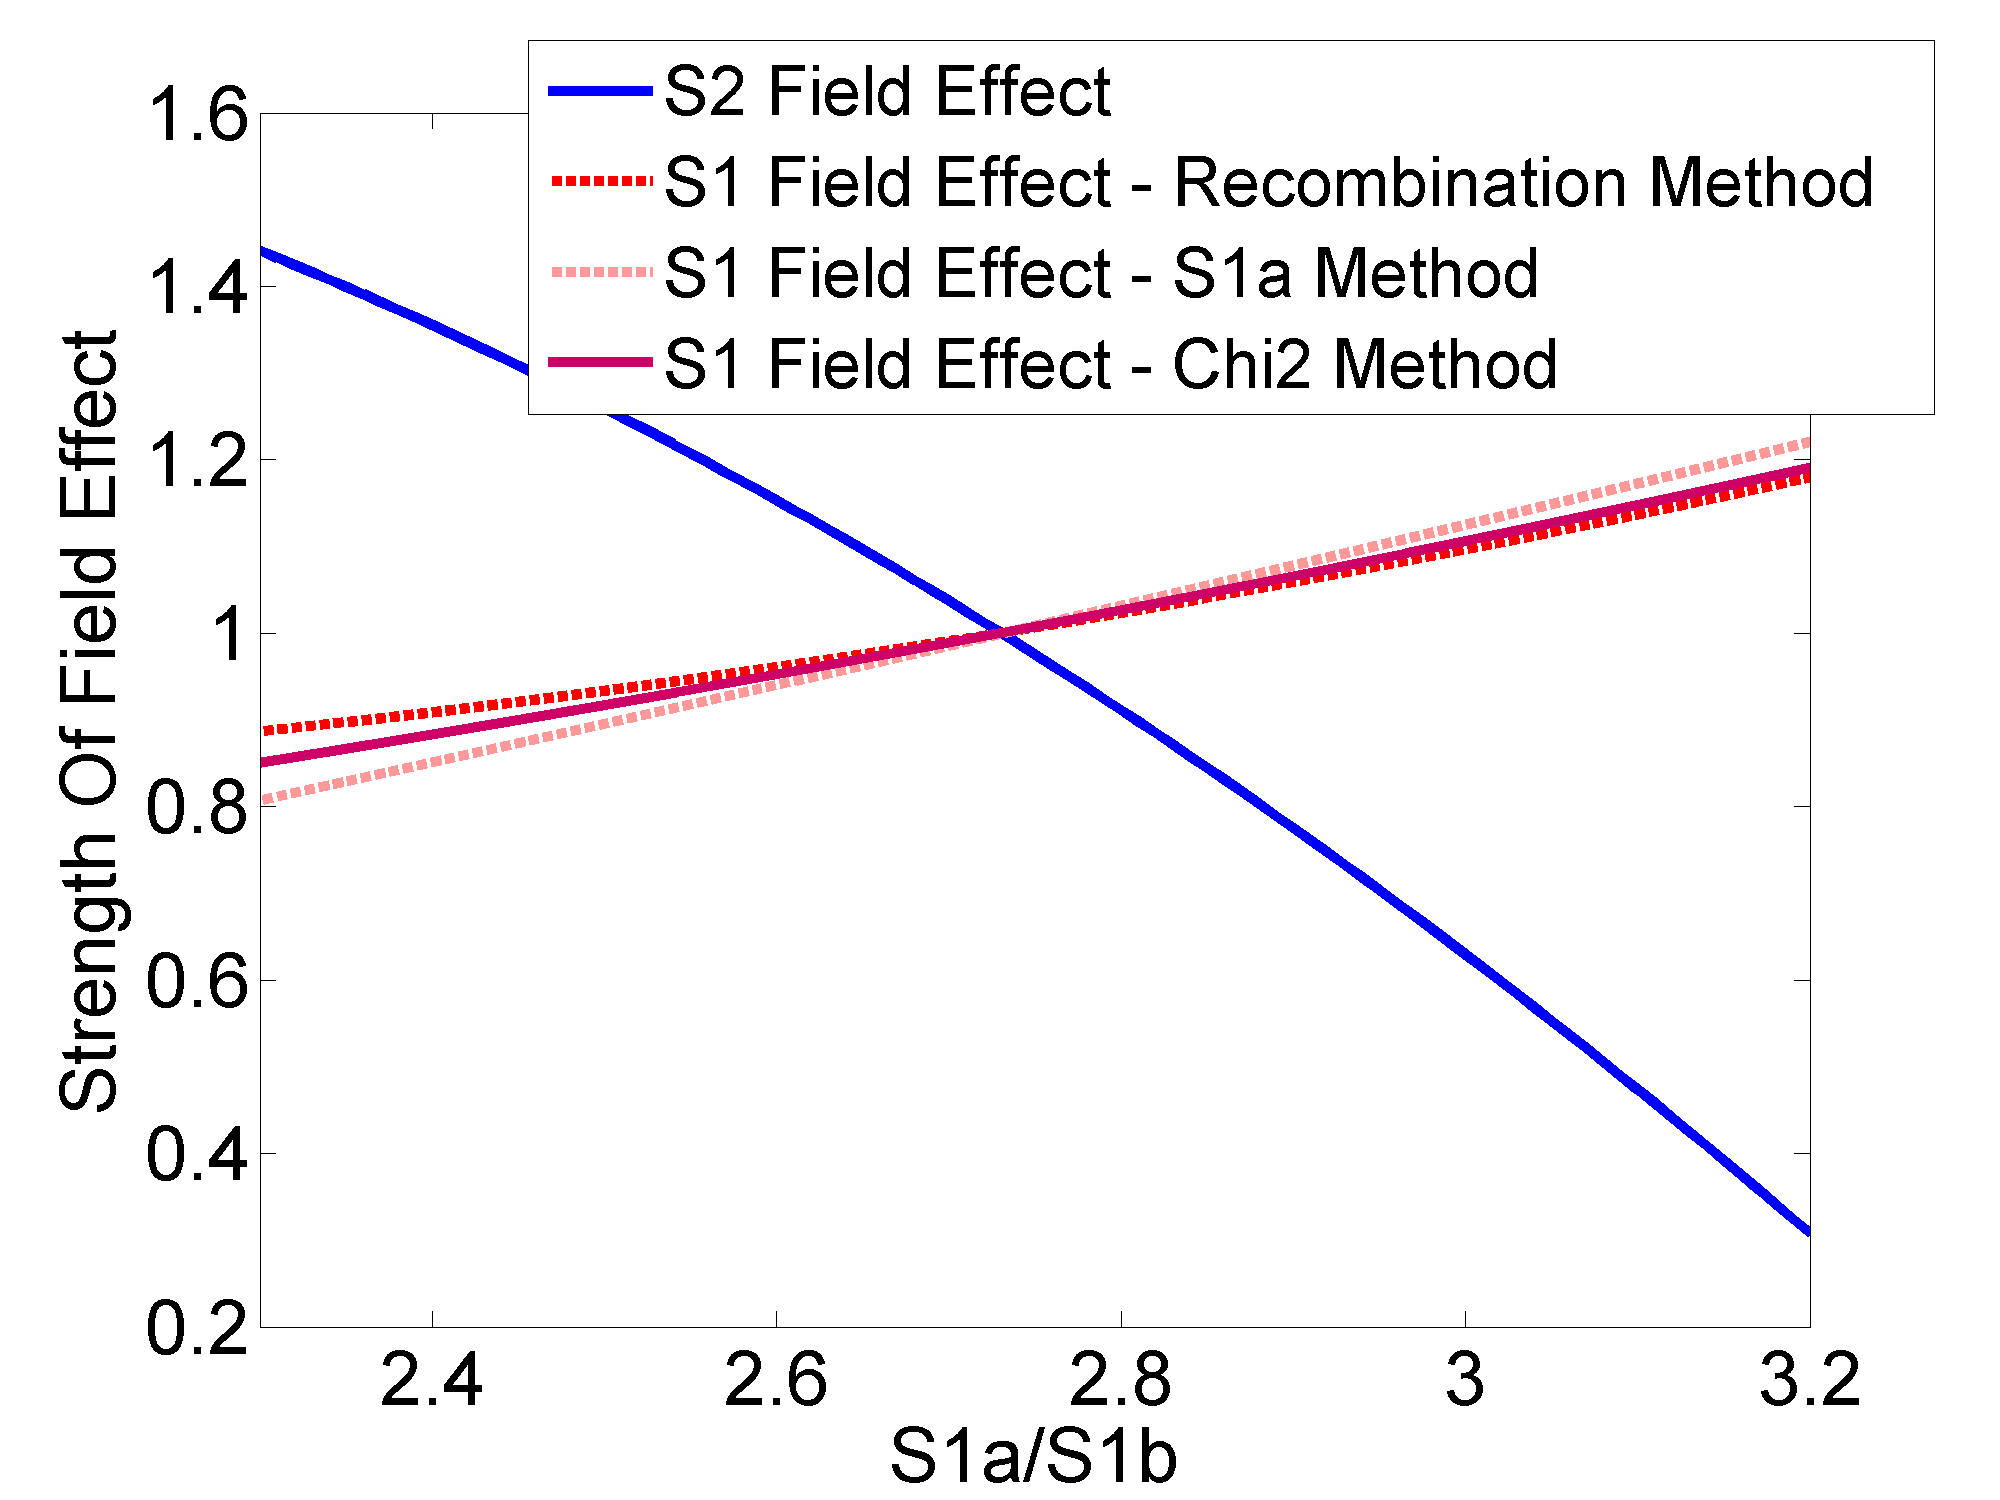
\includegraphics[scale=0.6]{Run04Corrections/StrengthOfFieldEffectOverlay.png}
\captionof{figure}{The S1a/S1b to field effect relationships measured in this work.  The method to measure each line is indicated by the color in the legend.  Red shades indicate measurements of the strength of the field effect in  $^{83m}$Kr S1 data, and blue shades indicate the strength of the field effect in  $^{83m}$Kr S2 data. Solid lines represent measurements that are used in KrypCal, and dashed lines represent measurements that are supplementary cross checks. }
 \label{AllMeasurements}
\end{figure}

\subsection{Producing Detector Inefficiency Corrections in KrypCal} \label{KrypCalCode}

Now that we have related the strength of the field effect in both $^{83m}$Kr S2 and $^{83m}$Kr S1 data to the S1a/S1b ratio we can make use of these relationships to produce detector inefficiency-only corrections during every $^{83m}$Kr calibration.  This process is very similar to (and in some ways, the reverse of) the process to measure the field effect in $^{83m}$Kr S2 data. Nevertheless, we will describe the process here for completeness and clarity.

\subsubsection{Mapping S1a/S1b}

For a $^{83m}$Kr calibration at any point in time, we begin by measuring the Z and XY dependence of the S1a/S1b ratio using the methods of section  \ref{section:S1aS1b1} and  \ref{section:S1aS1b2}.  We first divide the detector into drift times bins with a width chosen such that each bin has roughly 300 events.   A Gaussian distribution is fit to the S1a and S1b spectrum of each bin to determine the mean pulse areas versus Z.  A second order polynomial is fit to the ratio of the Gaussian means versus Z and is used to determine the S1a/S1b at any drift time in the detector.  The XY dependence of the S1a/S1b signal is found in a similar manner.  

We first remove the Z dependence of the S1a/S1b data by normalizing the polynomial fit found above to the detector center (defined by taking the mean drift time value of all $^{83m}$Kr events above 4 $\mu$s drift time). We then divide the detector into square, two dimensional XY bins with lengths defined such that each bin has roughly 300 events, and fit a Gaussian distribution to the S1a and S1b data of each bin.  The mean of the Gaussian distribution from each bin is used to construct an S1a/S1b XY dependence map, with a spline interpolation and extrapolation being used to determine the XY dependence between and outside of the bins.  

If the $^{83m}$Kr data set has enough statistics (more than 100,000 S1a/S1b events after cuts) a three dimensional S1a/S1b map is also constructed, and used in favor of the Z and XY maps. The detector is divided into three dimensional voxels with dimensions chosen such that each voxel has roughly 200 events.  A three dimensional map of S1a/S1b ratio is produced by fitting a Gaussian distribution to the S1a and S1b pulse area spectrum in each voxel.  A spline interpolation is used to determine the S1a/S1b ratio between the three dimensional voxels, and the S1a/S1b Z dependence map is used to extrapolate outside of the range of the voxels. 

\subsubsection{Removing the field effect from $^{83m}$Kr Data}

We use the $^{83m}$Kr S2 field effect to S1a/S1b relationship and S1 field effect to S1a/S1b relationship measured in sections \ref{section:FieldEffects} and \ref{section:S1relation2} to convert the Z, XY, and three dimensional maps of S1a/S1b into field effect maps for both S1 and S2 data.  The strength of the field effect is measured by $\frac{S1_E(xyz)}{S1_E(center)}$ and $\frac{S2_E(xyz)}{S2_E(center)}$, so that dividing by the strength of the field effect normalizes the raw $^{83m}$Kr S1 and S2 signals to the center of the detector and produces the field effect-only corrected S1$_F$ and S2$_F$ signals, as shown in equations \ref{S1F-2} and \ref{S2F-2}. (Figure \ref{fig:KrypCalFieldStrength})
\begin{align} 
S1_F &=S1 \times \frac{S1_E(center)}{S1_E(xyz)} \label{S1F-2} \\
S2_F &=S2 \times \frac{S2_E(center)}{S2_E(xyz)} \label{S2F-2}
\end{align}


\begin{figure}[!h]
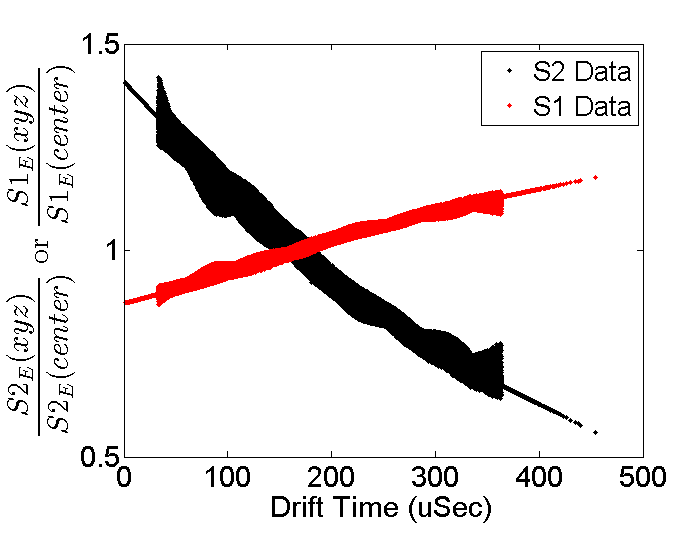
\includegraphics[scale=0.5]{Run04Corrections/KrypCal_FieldEffect.png}
\captionof{figure}{The three dimensional field effect in $^{83m}$Kr S2 (black) and S1(red) data versus drift time.  The wide regions are areas in which the three dimensional S1a/S1b maps are interpolated with a spline function, and the narrow regions are areas in which the three dimensional S1a/S1b maps are extrapolated based on the S1a/S1b Z dependence map.}\label{fig:KrypCalFieldStrength}
\end{figure}

\subsubsection{Measuring Detector Inefficiencies}


After removing the field effects from the $^{83m}$Kr data we are ready to measure the residual spatial pulse area variation due to detector inefficiencies alone.  We first measure the Z dependence of the S2$_F$ and S1$_F$ pulse areas by slicing the detector into drift time bins with widths defined such that each bin has roughly 300 events.  A Gaussian distribution is fit to the S2$_F$ and S1$_F$ spectra of each bin to determine the location of the spectra maxima. (Figure \ref{fig:KrypCal_S2ZDep} and Figure \ref{fig:KrypCal_S1ZDep}) In the case of the S2$_F$ signal, a cubic interpolation is used to determine the S2$_F$ Z dependence between each drift time bin, and a linear extrapolation based on the first and last 20\% of Gaussian distribution data points is used to determine the S2$_F$ Z dependence above and below the span of the drift time bins.  

A detector inefficiency correction for the Z direction is defined by taking the ratio of the S2$_F$  pulse area at a height of 4 $\mu$s (just below the liquid surface) to the S2$_F$ pulse area as a function of Z as described in the equation
\begin{equation}
\mbox{S}2_{\mbox{z-efficiency-correction}} = \frac{S2_F(z=4)}{S2_F(z)}.
\end{equation} 
In the case of the S1$_F$ signal, a second order polynomial is used to determine the S1$_F$ Z dependence between and outside of each drift time bin. A detector inefficiency correction for the Z direction is defined by taking the ratio of the S1$_F$  pulse area at the center of the detector ($z_c$ as defined by the average drift time of $^{83m}$Kr) to the S1$_F$ pulse area as a function of Z as described in the equation
\begin{equation}
\mbox{S}1_{\mbox{z-efficiency-correction}} = \frac{S1_F(z_c)}{S1_F(z)}.
\end{equation} 

\begin{figure}[!h]
\centering
\subfloat{{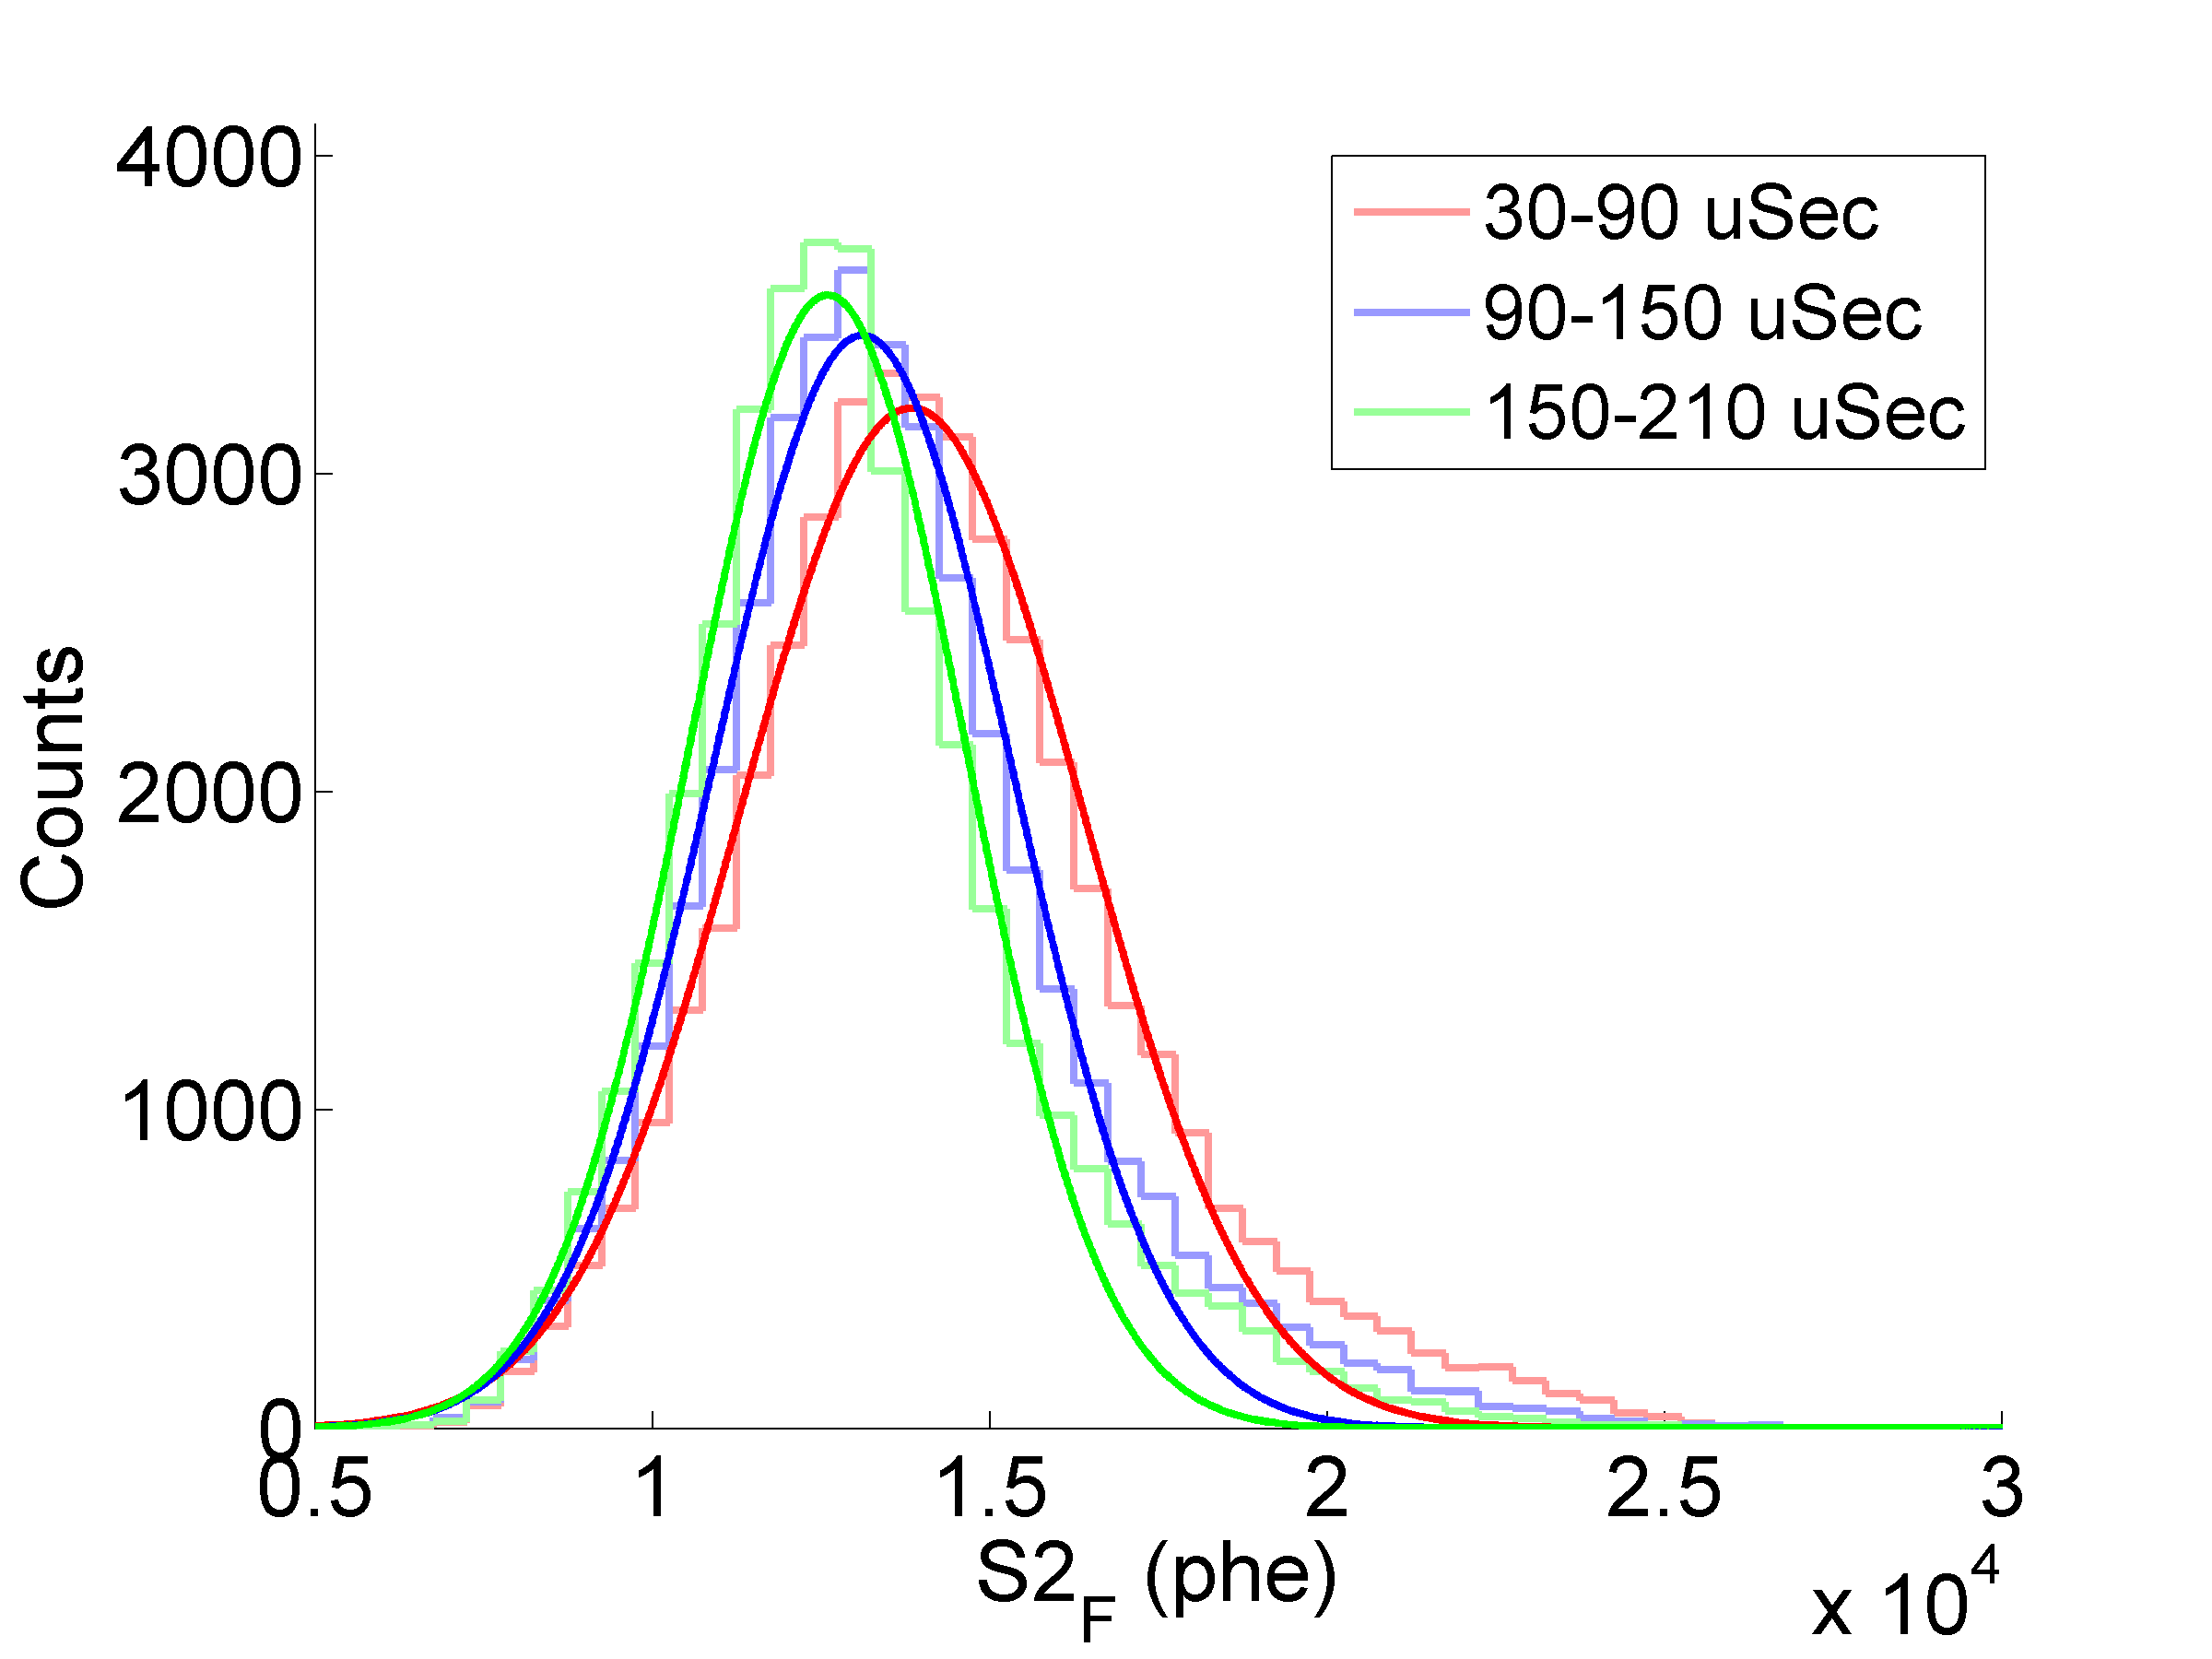
\includegraphics[width=6.5cm]{Run04Corrections/S2F_GaussianFits.png} }}
\qquad
\subfloat{{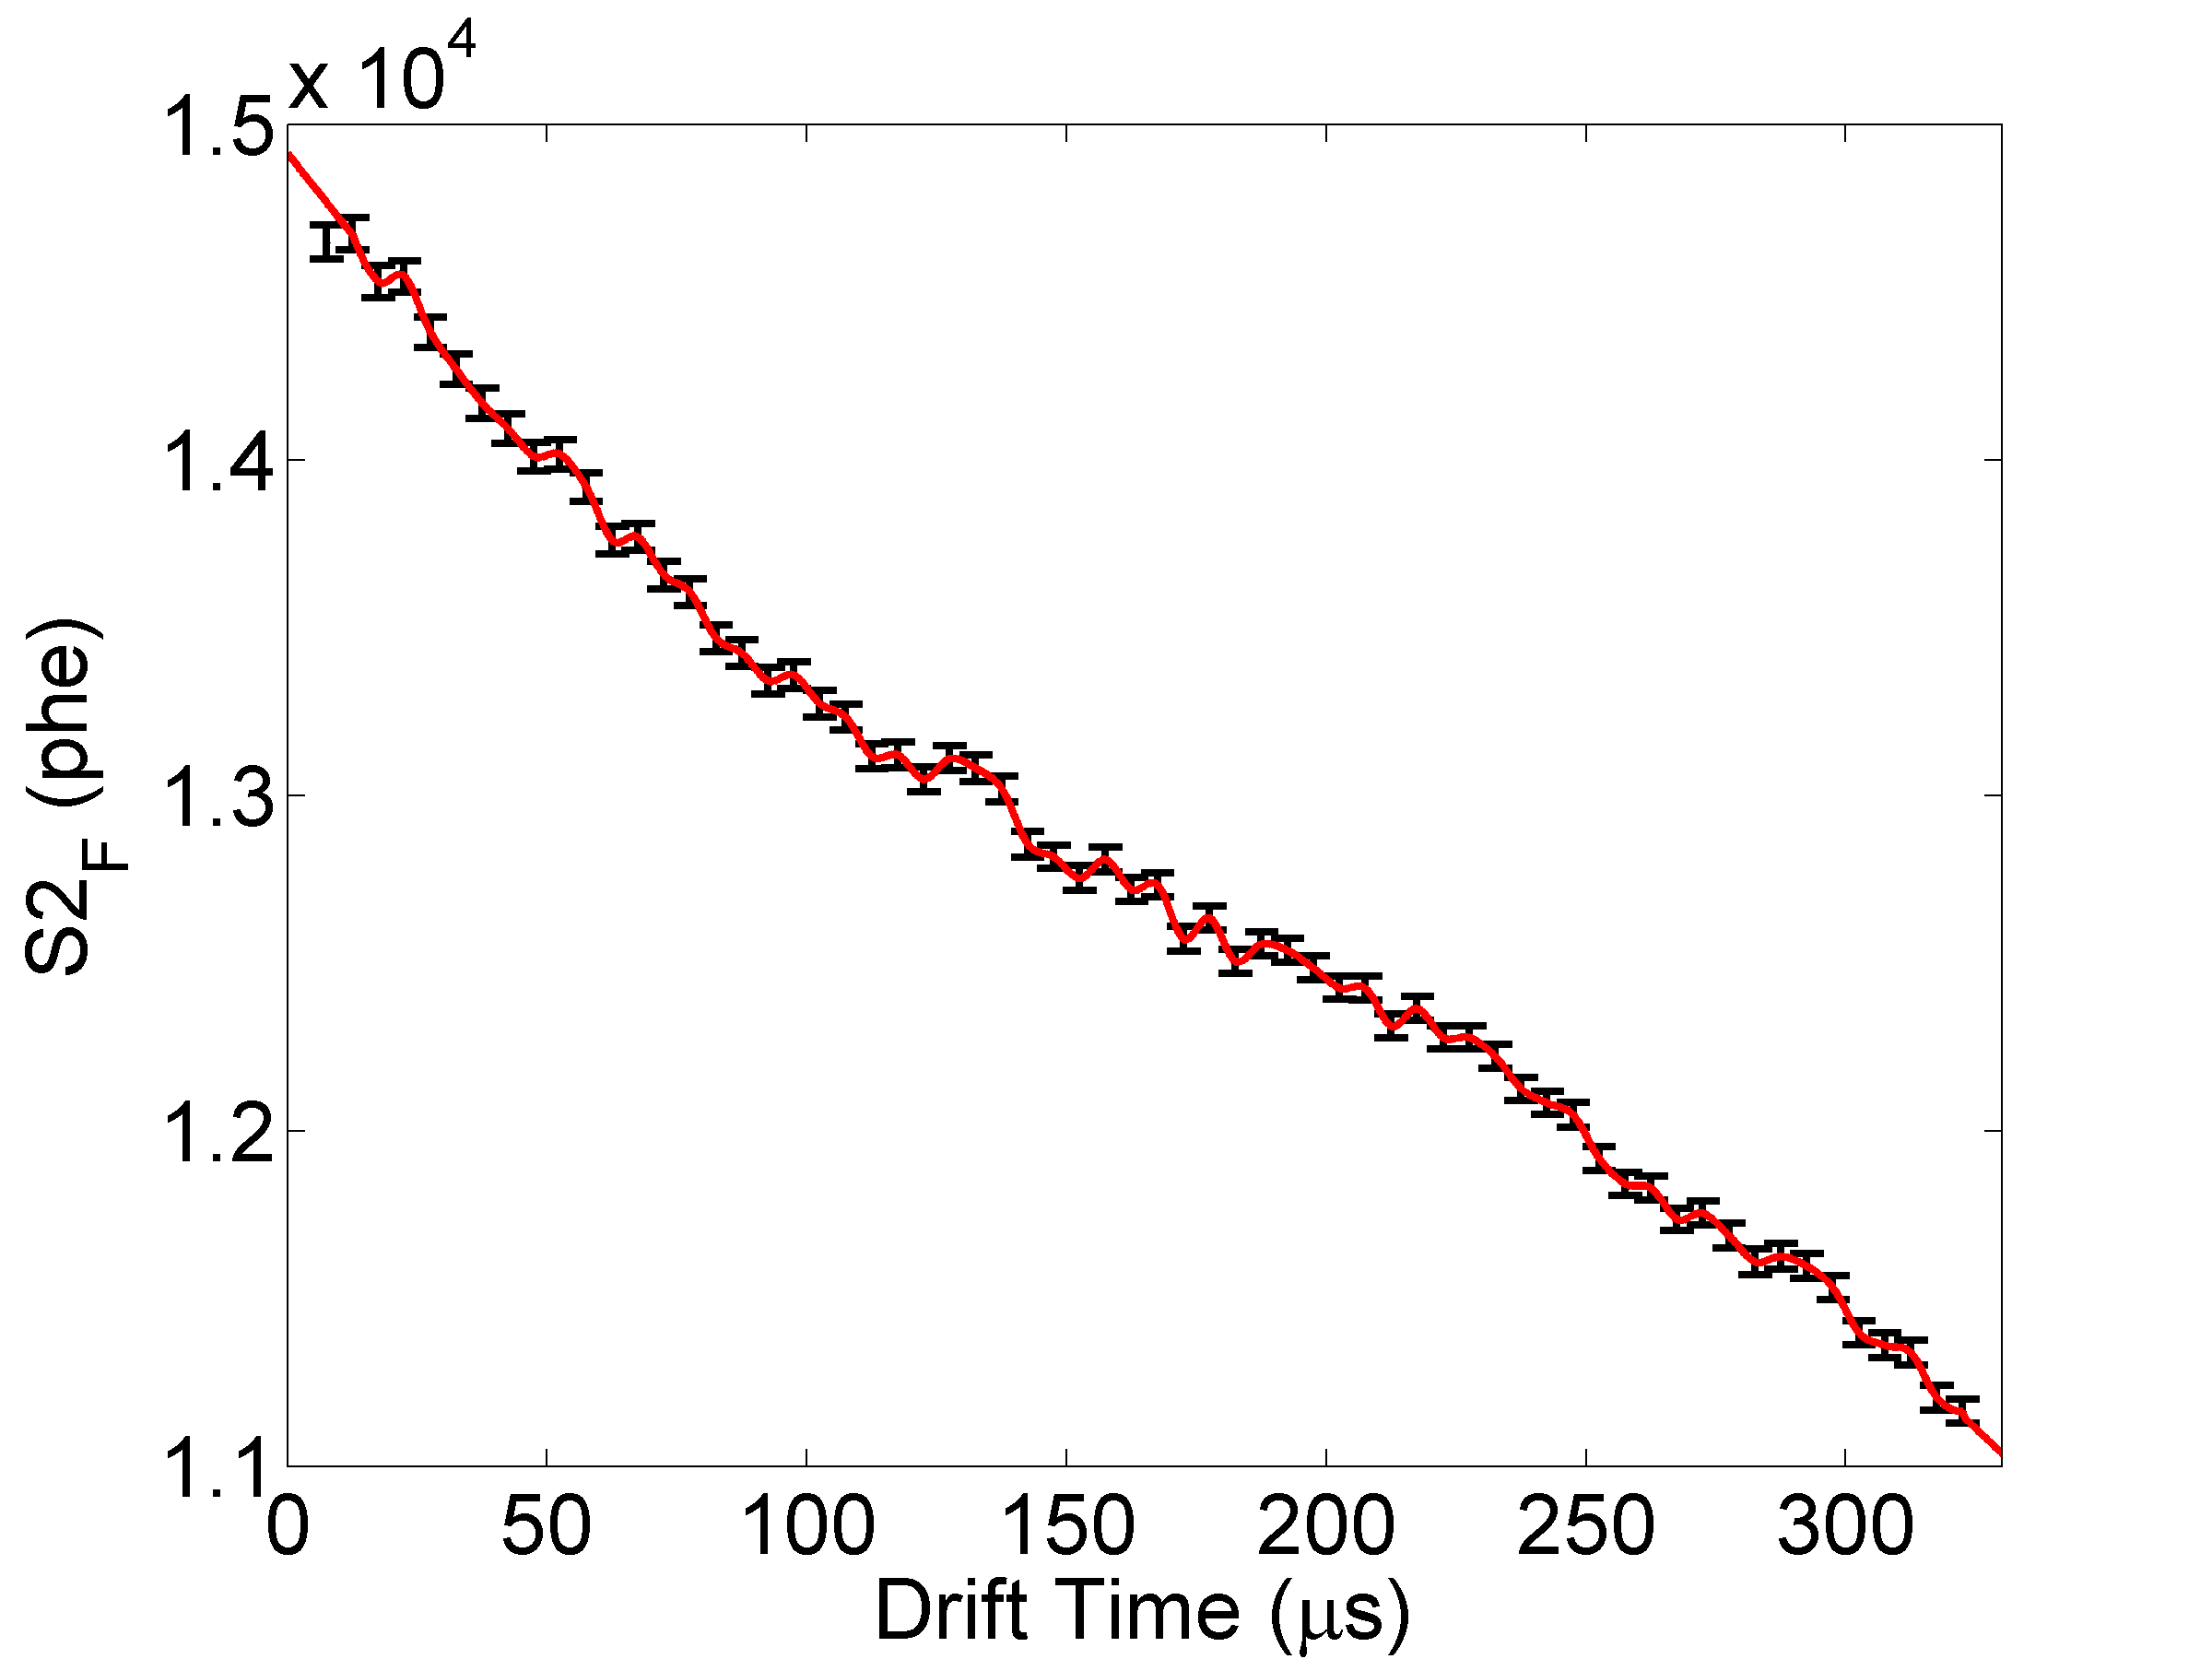
\includegraphics[width=6.5cm]{Run04Corrections/S2F_ZDep.png} }}
\captionof{figure}{ (Left) Gaussian distribution fits to the field corrected S2$_F$ data that are used to determine the drift time dependence of the S2$_F$ pulse area. For illustrative purposes, a drift time bin width of 60 $\mu$s was chosen for this plot. (Right) The Z dependence of the S2$_F$ pulse area after field effects are removed.  Black points indicate the maximum of Gaussian distribution fits for each drift time bin, and the red line indicate the interpolation and extrapolation of that data.}
\label{fig:KrypCal_S2ZDep}
\end{figure}

\begin{figure}[!h]
\centering
\subfloat{{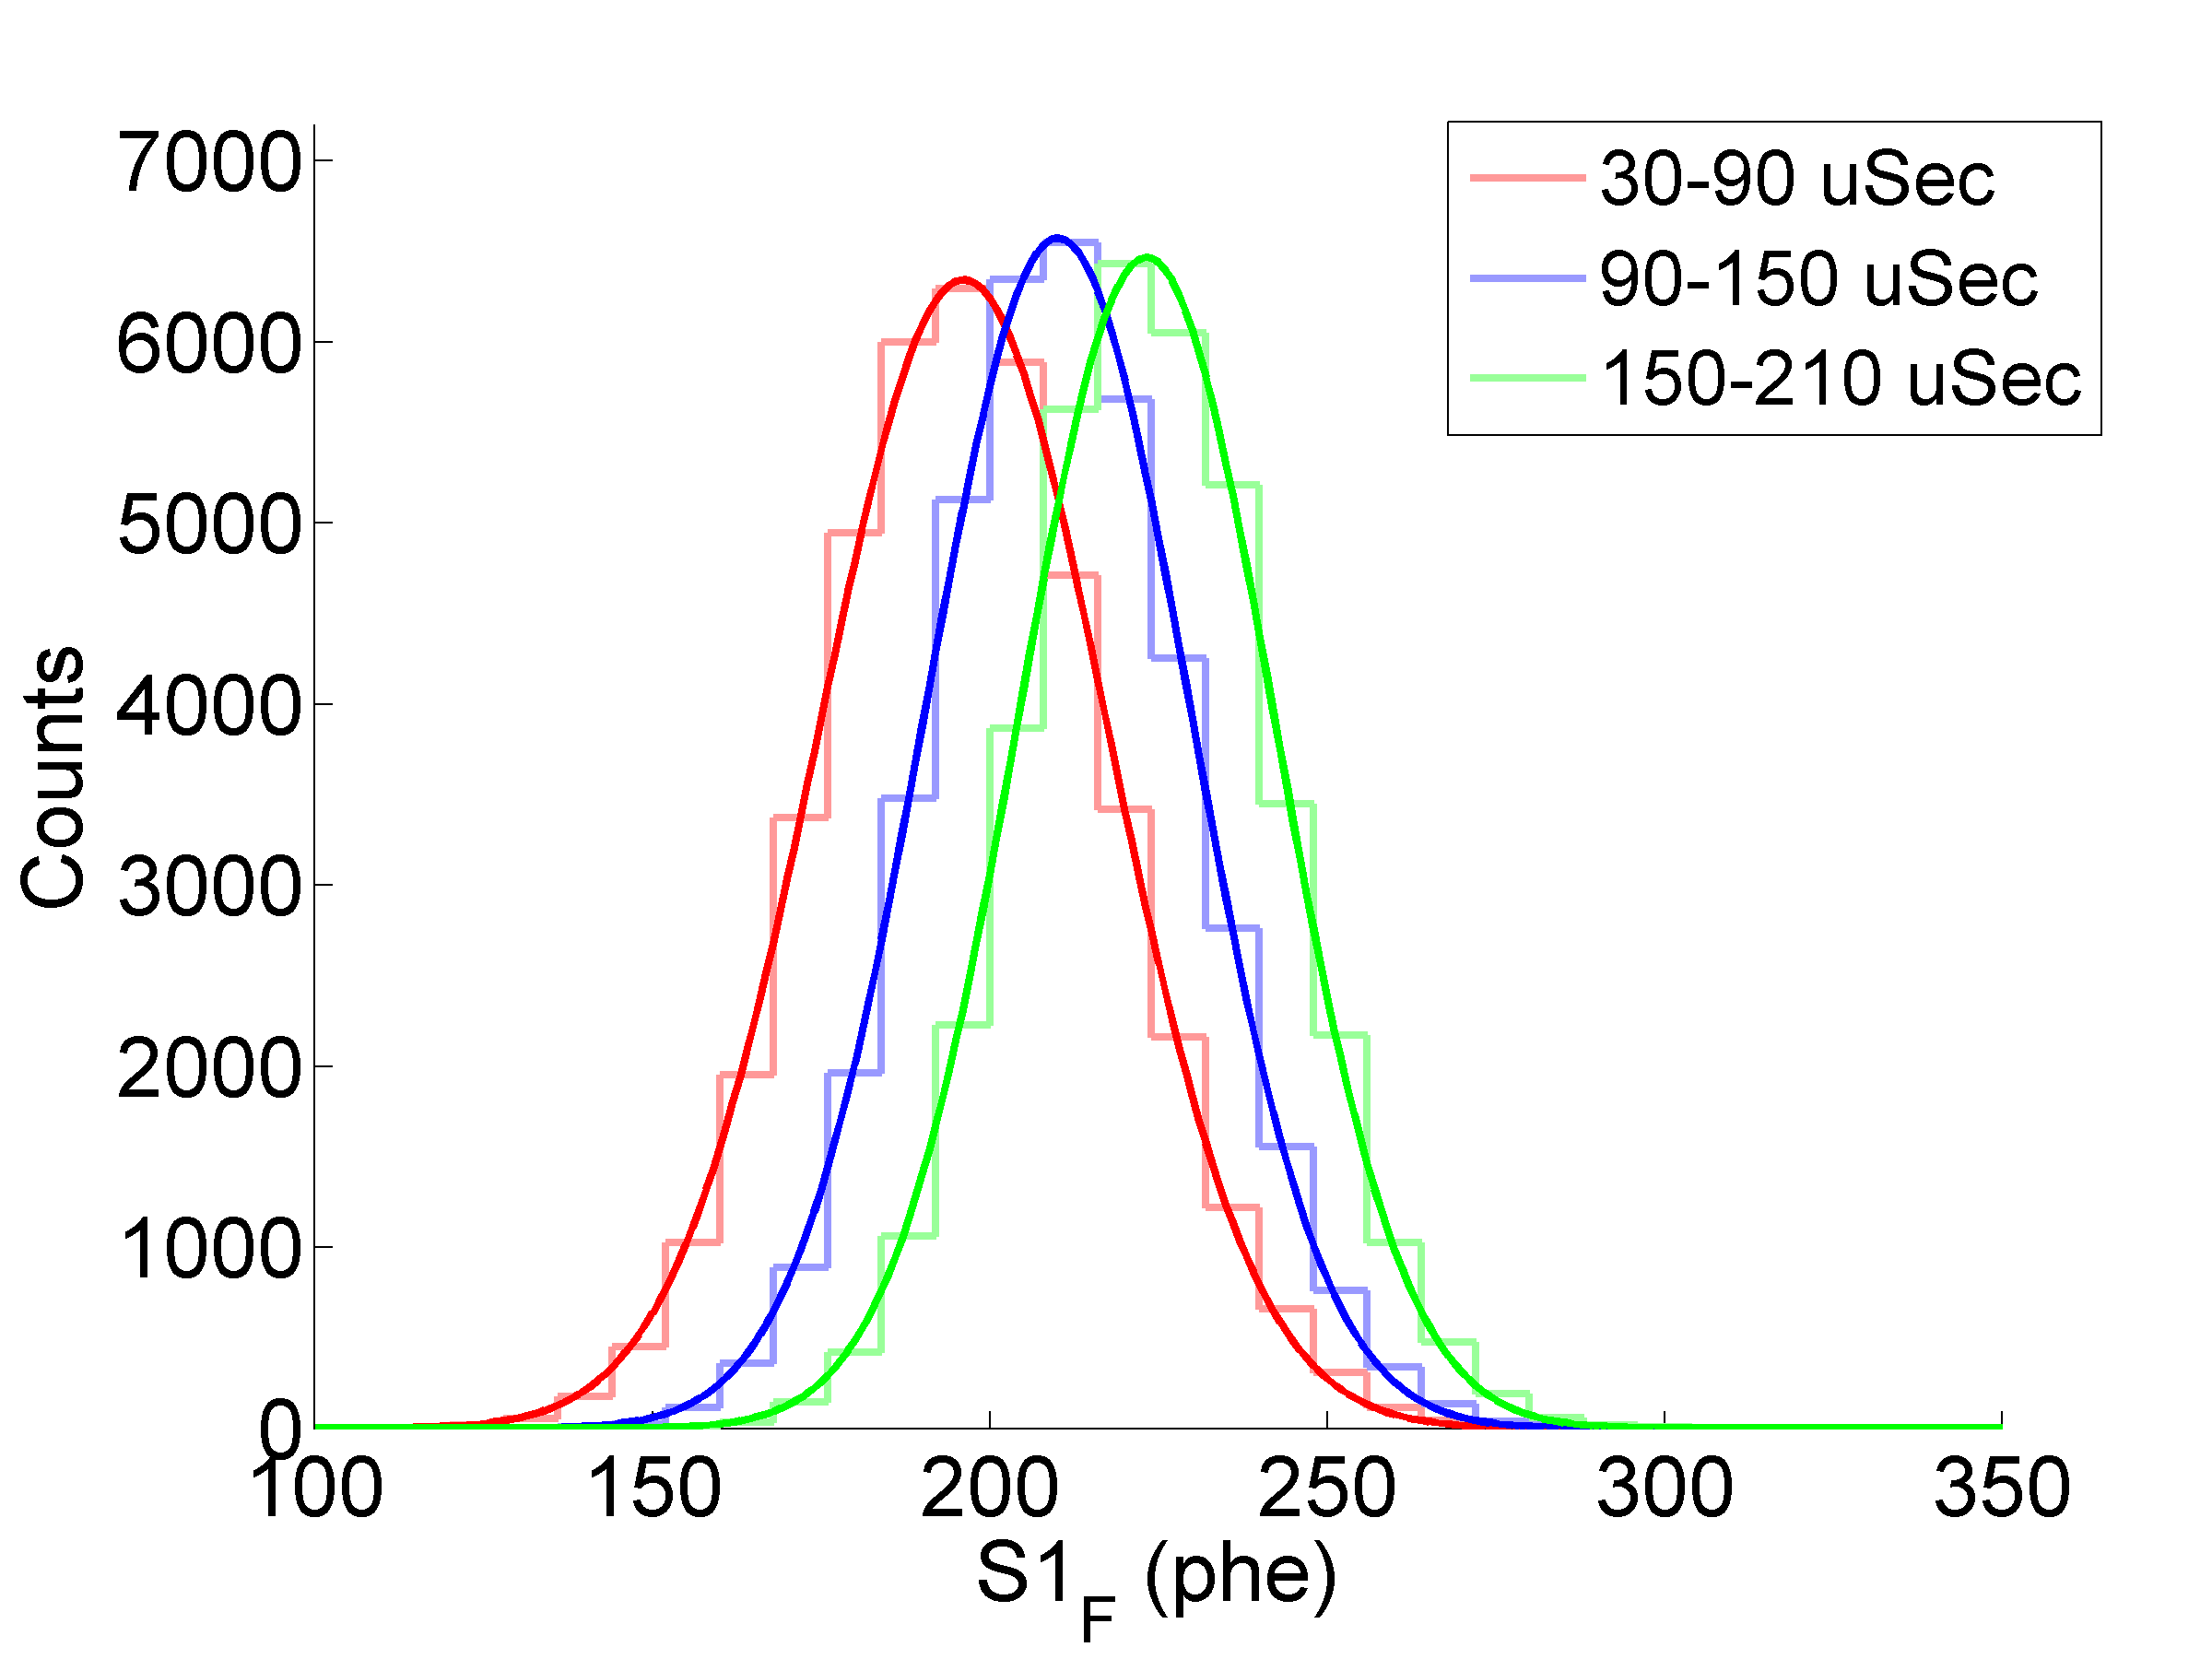
\includegraphics[width=6.5cm]{Run04Corrections/S1F_GaussianFits.png} }}
\qquad
\subfloat{{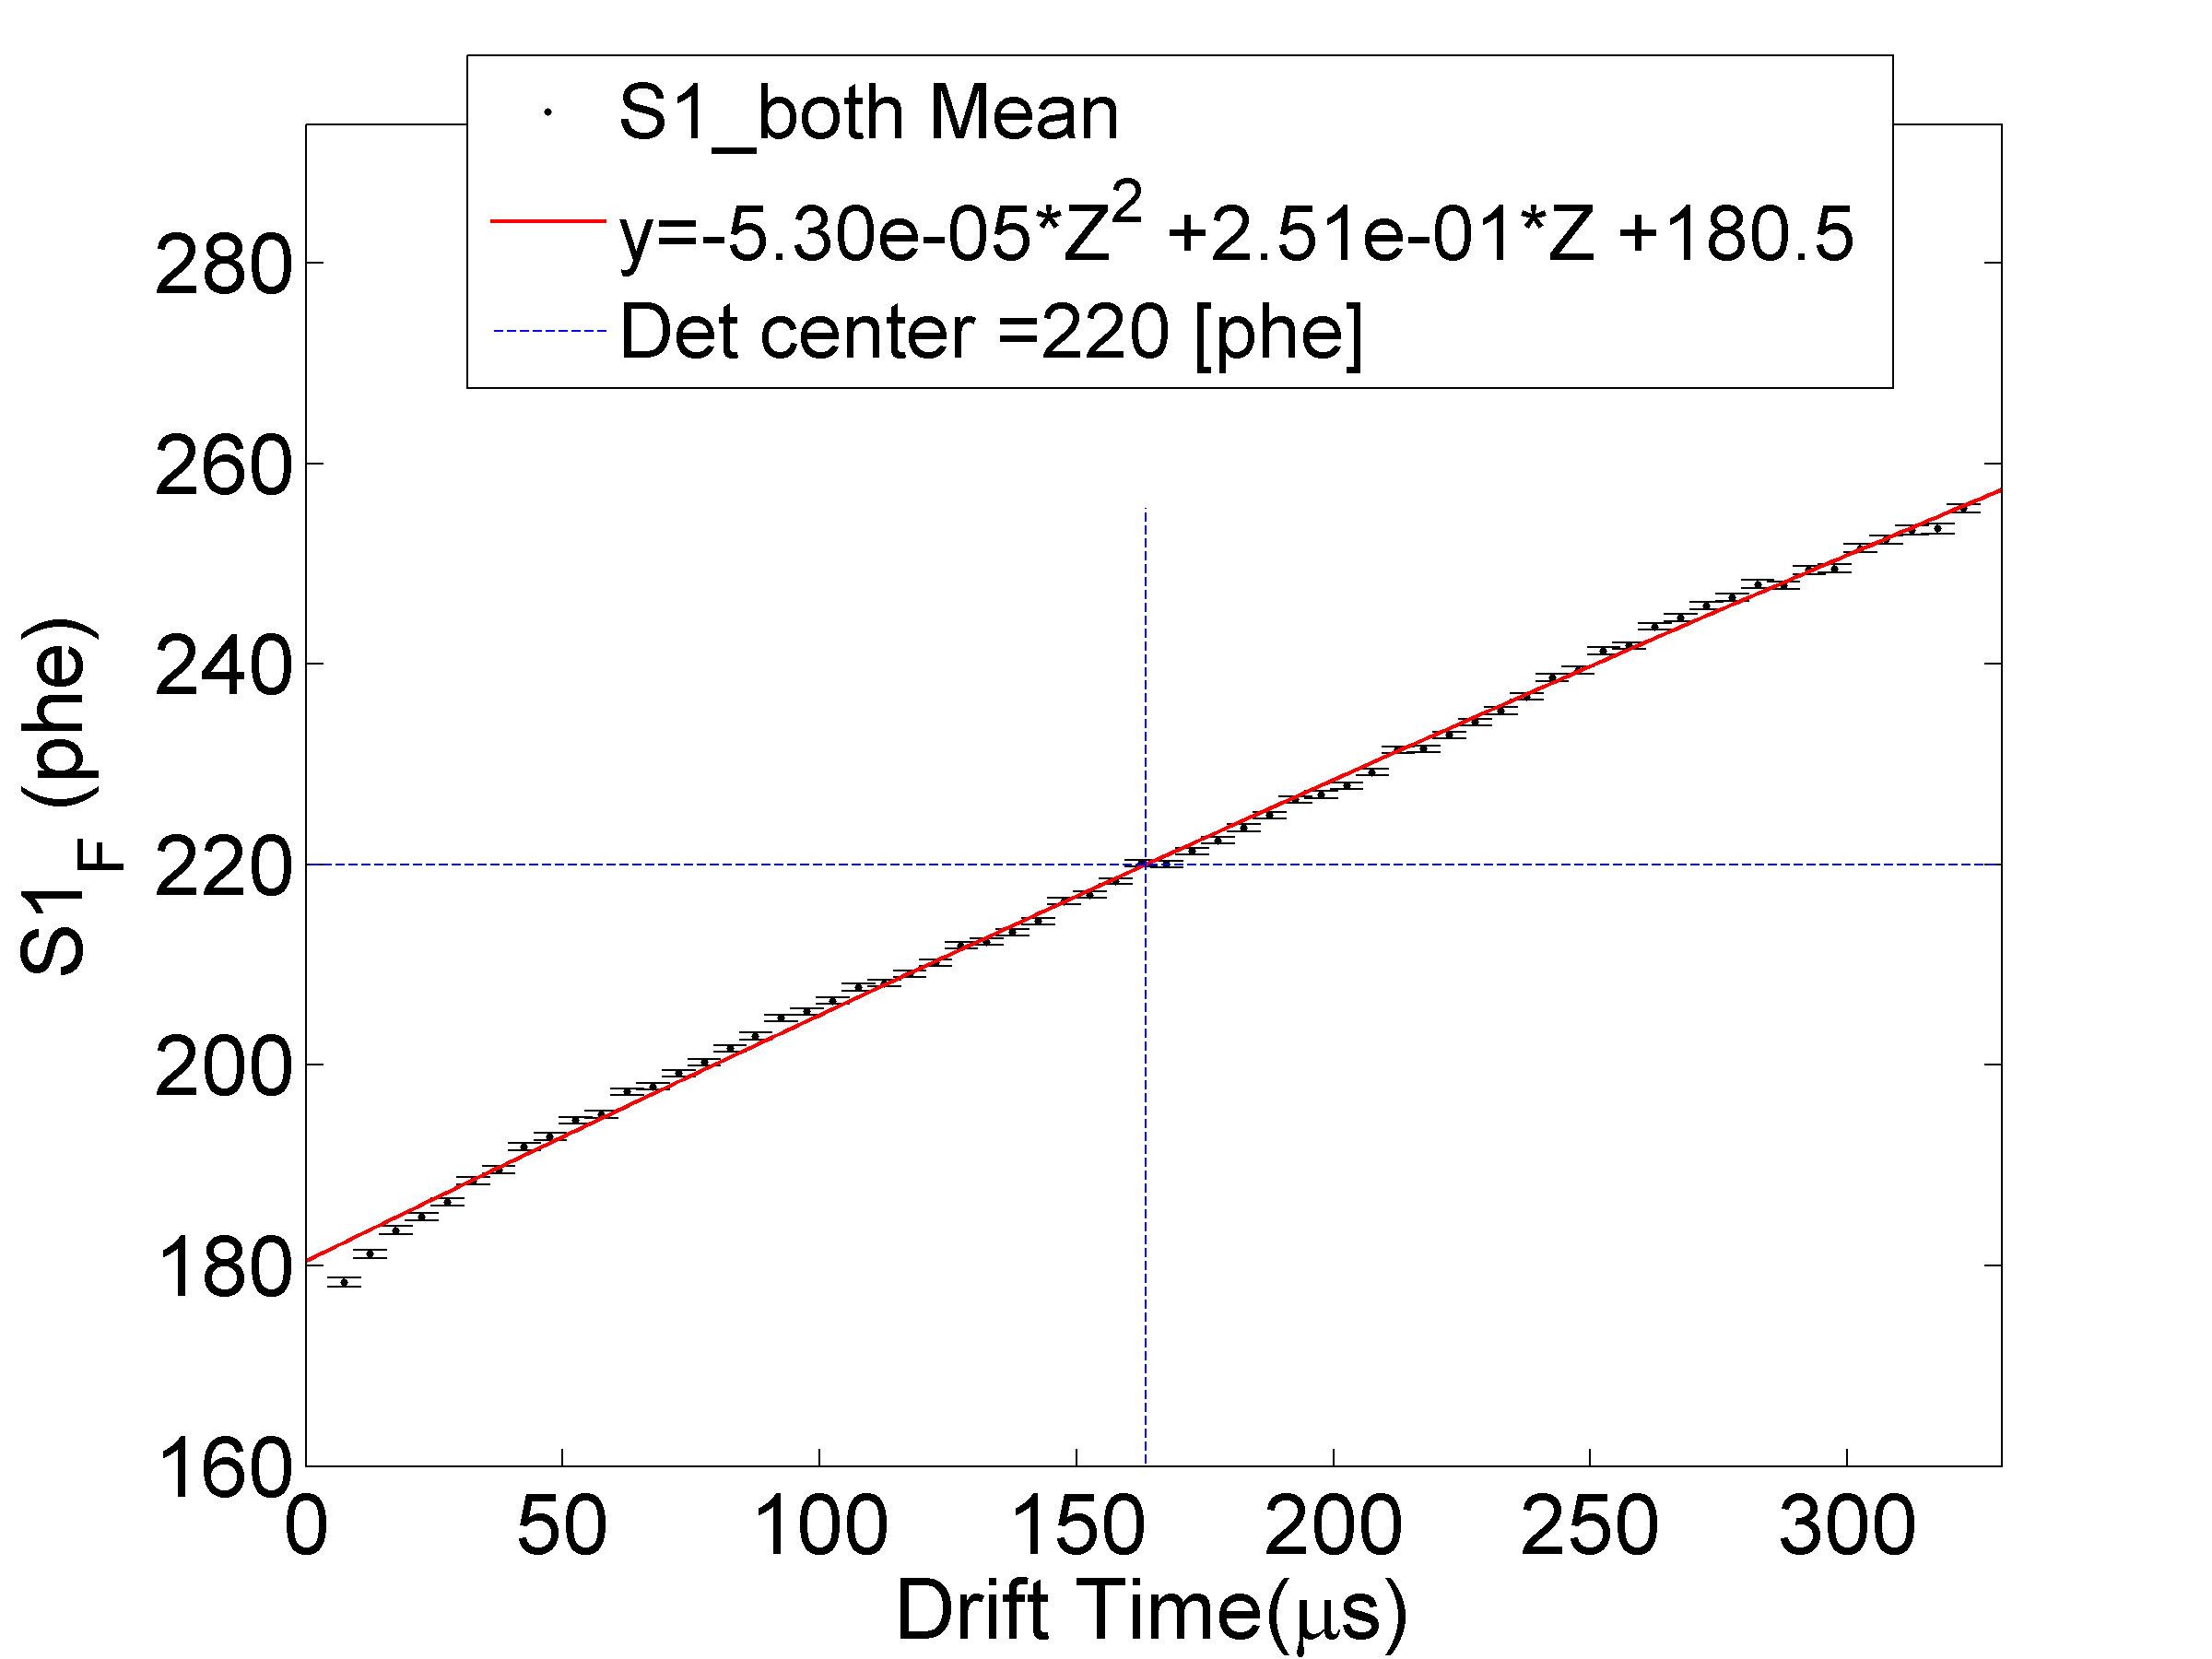
\includegraphics[width=6.5cm]{Run04Corrections/S1F_ZDep.png} }}
\captionof{figure}{ (Left)  Gaussian distribution fits to the field corrected S1$_F$ data that are used to determine the drift time dependence of the S1$_F$ pulse area. For illustrative purposes, a drift time bin width of 60 $\mu$s was chosen for this plot. (Right) The Z dependence of the S1$_F$ pulse area after field effects are removed.  Black points indicate the maximum of Gaussian distribution fits for each drift time bin, and red line indicates the second order polynomial fit to that data.}
\label{fig:KrypCal_S1ZDep}
\end{figure}

The XY dependence of the field removed S2$_F$ and S1$_F$ signals are found by dividing the z inefficiency corrected (S2$_F \times \mbox{S}2_{\mbox{z-efficiency-correction}}$ and S1$_F \times \mbox{S}1_{\mbox{z-efficiency-correction}}$) data into two dimensional XY bins with lengths defined such that each bin has roughly 300 events, and then fitting Gaussian distributions to the data of each bin.  The mean of the Gaussian distribution from each bin is used to construct S2$_F$ and S1$_F$ XY dependence maps, with a spline interpolation and extrapolation being used to determine the XY dependence between and outside of the bins. (Figure \ref{fig:KrypCalXYDep}) A detector inefficiency correction for the XY direction is defined by taking the ratio of the z inefficiency corrected S2$_F$ (or S1$_F$) pulse area at the center of the detector to the z inefficiency corrected S2$_F$ (or S1$_F$) pulse area as a function of XY in cm, as shown below
\begin{align}
\mbox{S}2_{\mbox{xy-efficiency-correction}} &= \frac{\mbox{S}2_{\mbox{z-efficiency-correction}}\times S2_F(x_c,y_c,z)}{\mbox{S}2_{\mbox{z-efficiency-correction}}\times S2_F(xyz)} \\
\mbox{S}1_{\mbox{xy-efficiency-correction}} &= \frac{\mbox{S}1_{\mbox{z-efficiency-correction}}\times S1_F(x_c,y_c,z)}{\mbox{S}1_{\mbox{z-efficiency-correction}}\times S1_F(xyz)}.
\end{align} 
where $x_c$ and $y_c$ are the x and y center of the detector in uncorrected coordinates determined by taking the average position of the $^{83m}$Kr events in each direction.

\begin{figure}[!h]
\centering
\subfloat{{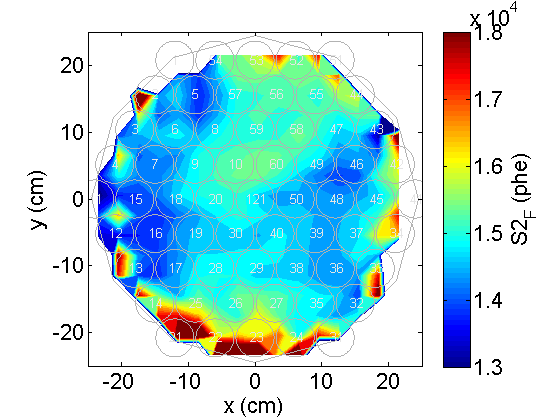
\includegraphics[width=6.5cm]{Run04Corrections/S2F_XYDep.png} }}
\qquad
\subfloat{{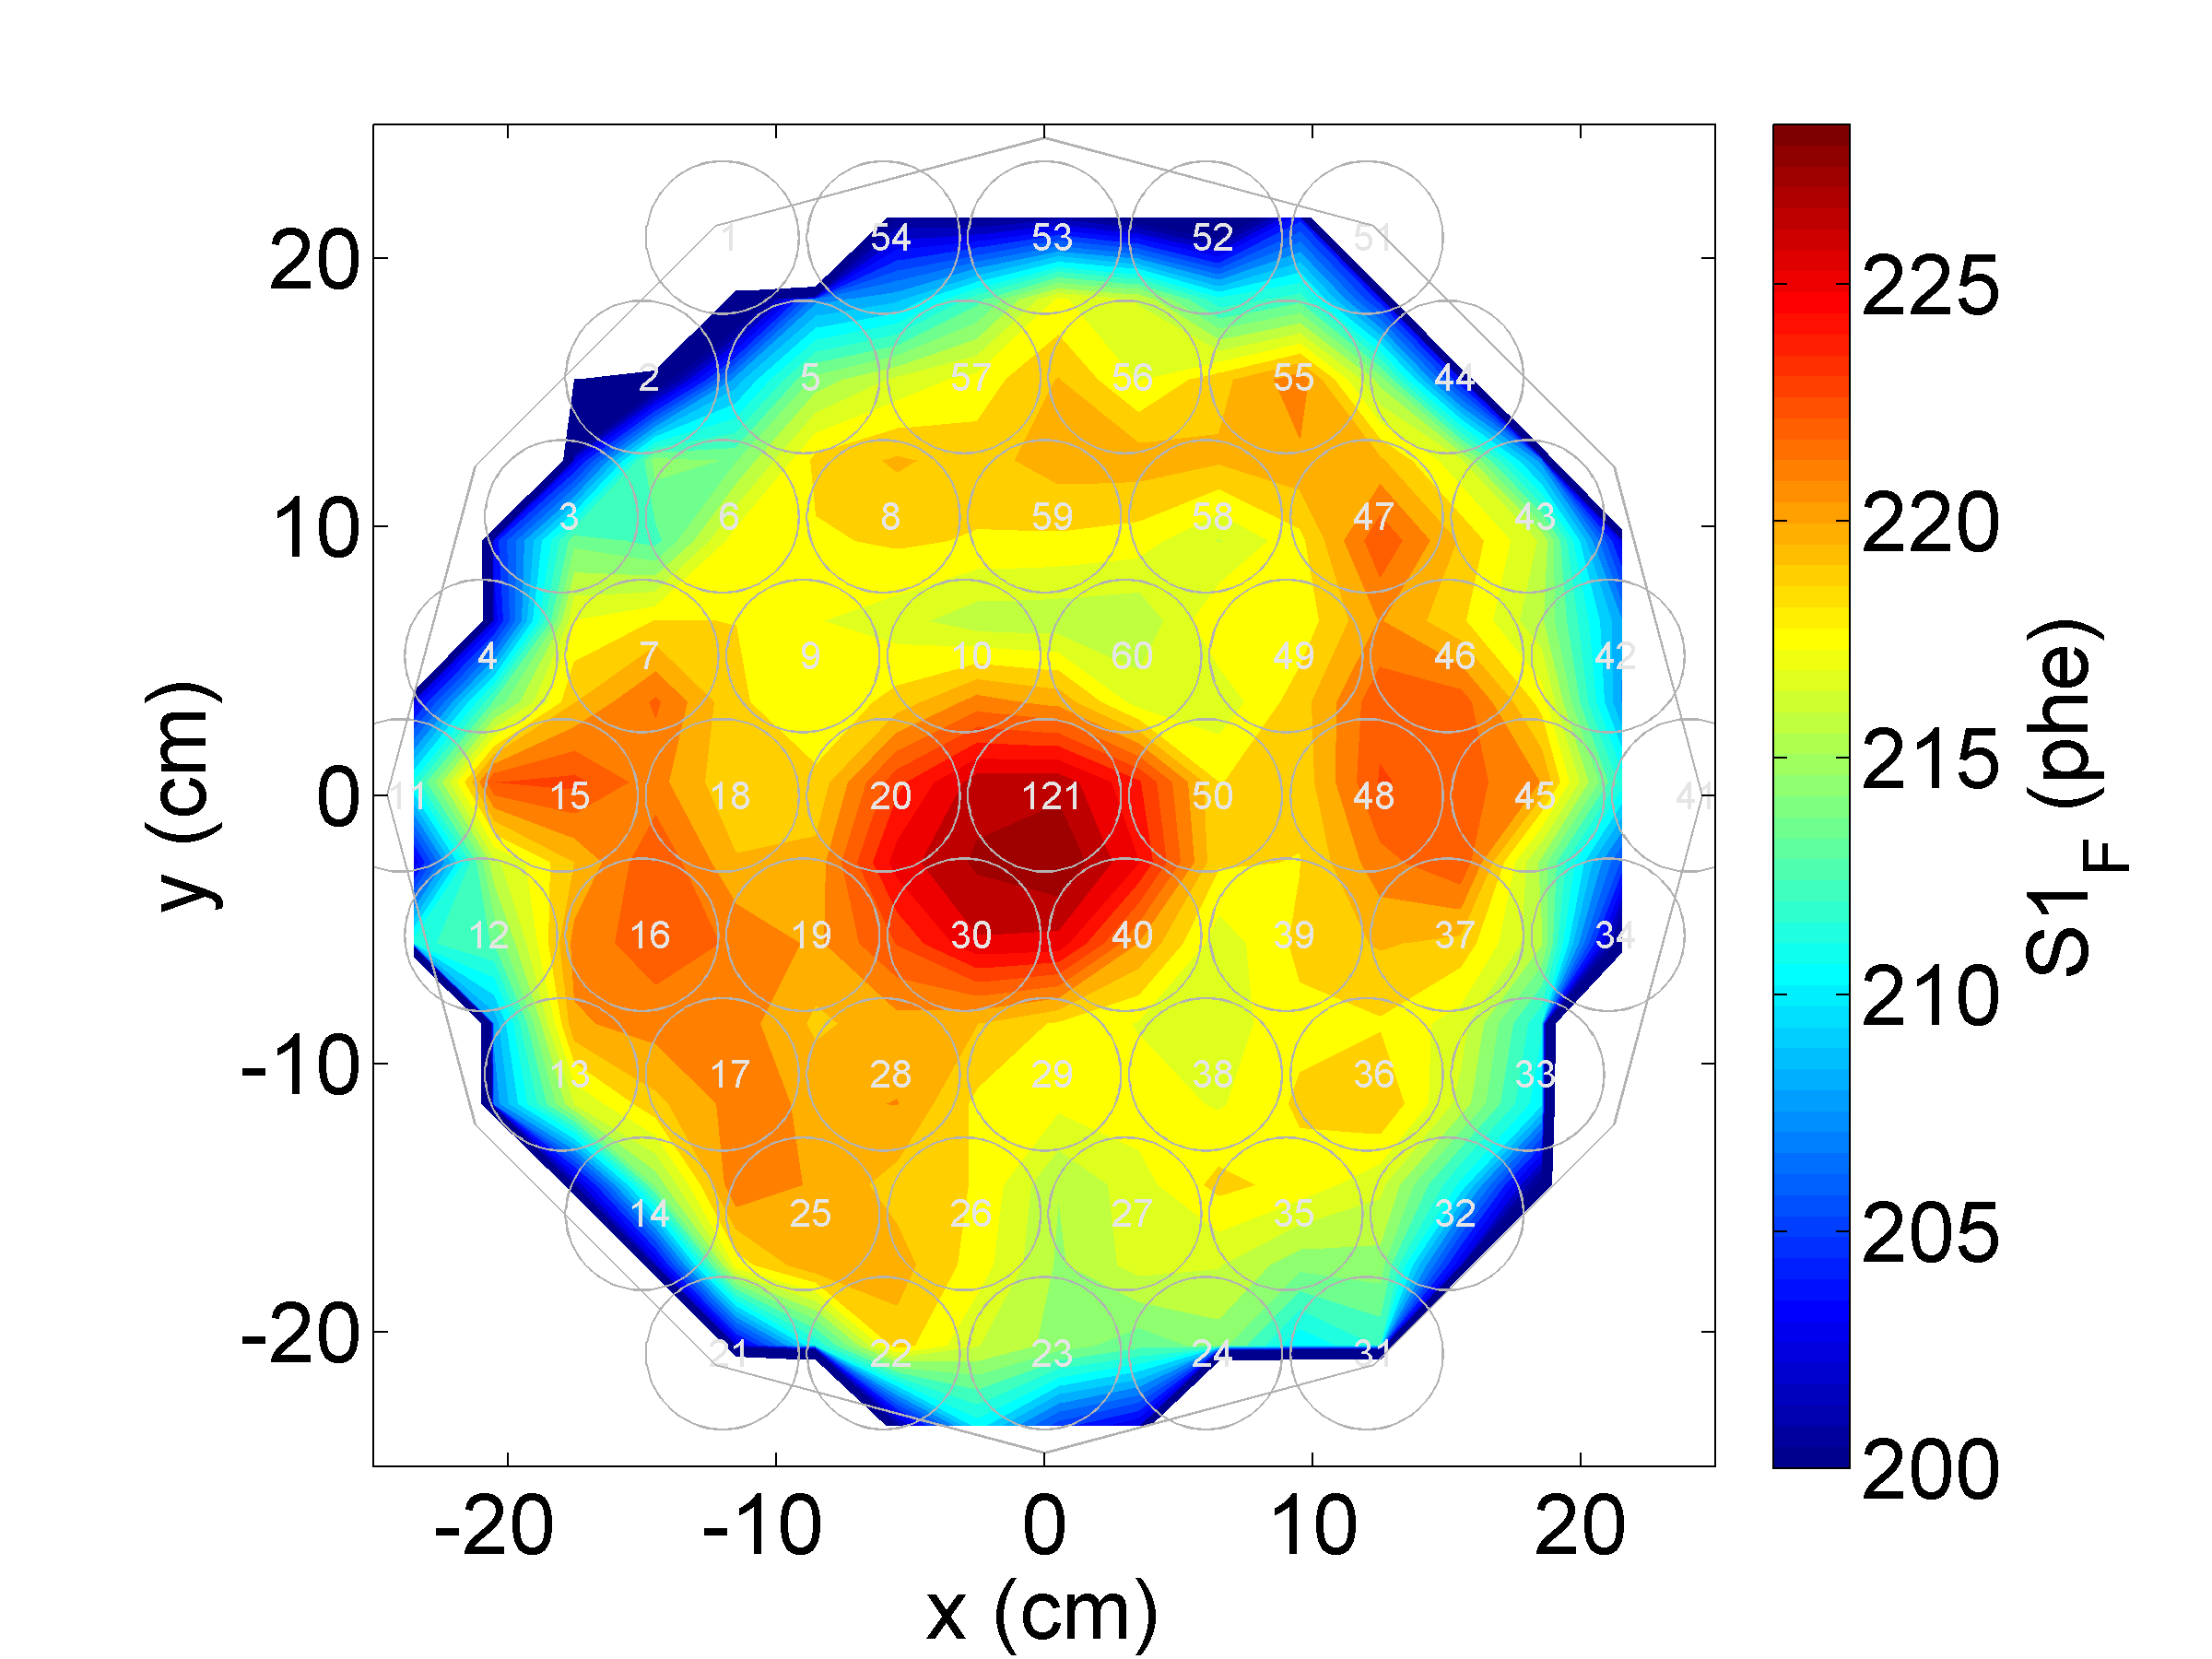
\includegraphics[width=6.5cm]{Run04Corrections/S1F_XYDep.png} }}
\captionof{figure}{ (Left) Two dimensional map of the XY dependence in $^{83m}$Kr S2$_F$ data determine by fitting a Gaussian distribution to XY bins of the data and tracking the mean of each fit.(Right) Two dimensional map of the XY dependence in $^{83m}$Kr S1$_F$ data determine by fitting a Gaussian distribution to XY bins of the data and tracking the mean of each fit.}
\label{fig:KrypCalXYDep}
\end{figure}

To apply these S1 and S2 efficiency corrections to data at any time, we must interpolate between the corrections in time.  The S2$_E$ XY, S1$_E$ Z, and S1$_E$ XY efficiency corrections are not expected to change rapidly in time, so a simple nearest neighbor interpolation is used to apply these efficiency corrections to data sets at any point in time.  However, the S2$_E$ Z dependence is expected to change rapidly in time due to the sudden changes in xenon purity introduced by detector operations.  To account for this, we find the $^{83m}$Kr calibration taken immediately before and after a particular data set which the detector efficiency corrections are being applied to.  A weighted average of the $^{83m}$Kr S2$_E$ Z dependence splines, with weights based on the time between each $^{83m}$Kr calibration data set and the data set being corrected, is used to defined a time interpolate S2$_E$ Z dependence correction.  Multiplying the raw S2 and S1 signals of any data set by the time-interpolated Z and the XY correction factors results in inefficiency corrected S2$_E$ and S1$_E$ signals (with field effects still present).
\begin{align}
S2_E &=S2 \times \mbox{S}2_{\mbox{xy-efficiency-correction}} \times \mbox{S}2_{\mbox{z-efficiency-correction}} \\
S1_E &=S1 \times \mbox{S}1_{\mbox{xy-efficiency-correction}} \times \mbox{S}1_{\mbox{z-efficiency-correction}}
\end{align}

\subsubsection{Additional Output from the Corrections Module: Electron Lifetime}

The S2$_F$ Z dependence is not expected to be exponential in a nonuniform drift field due to the drift velocity dependent absorption cross section.  Nonetheless, it is still useful to define an approximate electron lifetime to track the purity of the detector's xenon over time.  Two approaches have been taken in this regard.  The first approach is to treat the S2$_F$ Z dependence as approximately exponential anyway and quote the exponential decay constant as the lifetime, regardless of the quality of the fit.  Due to the increasing strength of the field this approximation worsens over time. (Figure \ref{ELFits})  The second approach to measuring the electron lifetime is to define a pseudo-lifetime from the S2$_F$ Z dependence by fitting an exponential to the S2$_F$ mean just below the liquid surface (at 4 $\mu$s) and just above the cathode (at 320 $\mu$s).  While this approach avoids any issues with poor fits, it also neglects the S2$_F$ Z dependence in the bulk of the detector.  Note that the actual corrections use a spline fit to the S2$_F$ Z dependence, and therefore avoid any issues in defining an exponential lifetime.


\begin{figure}[!h]
\centering
\subfloat{{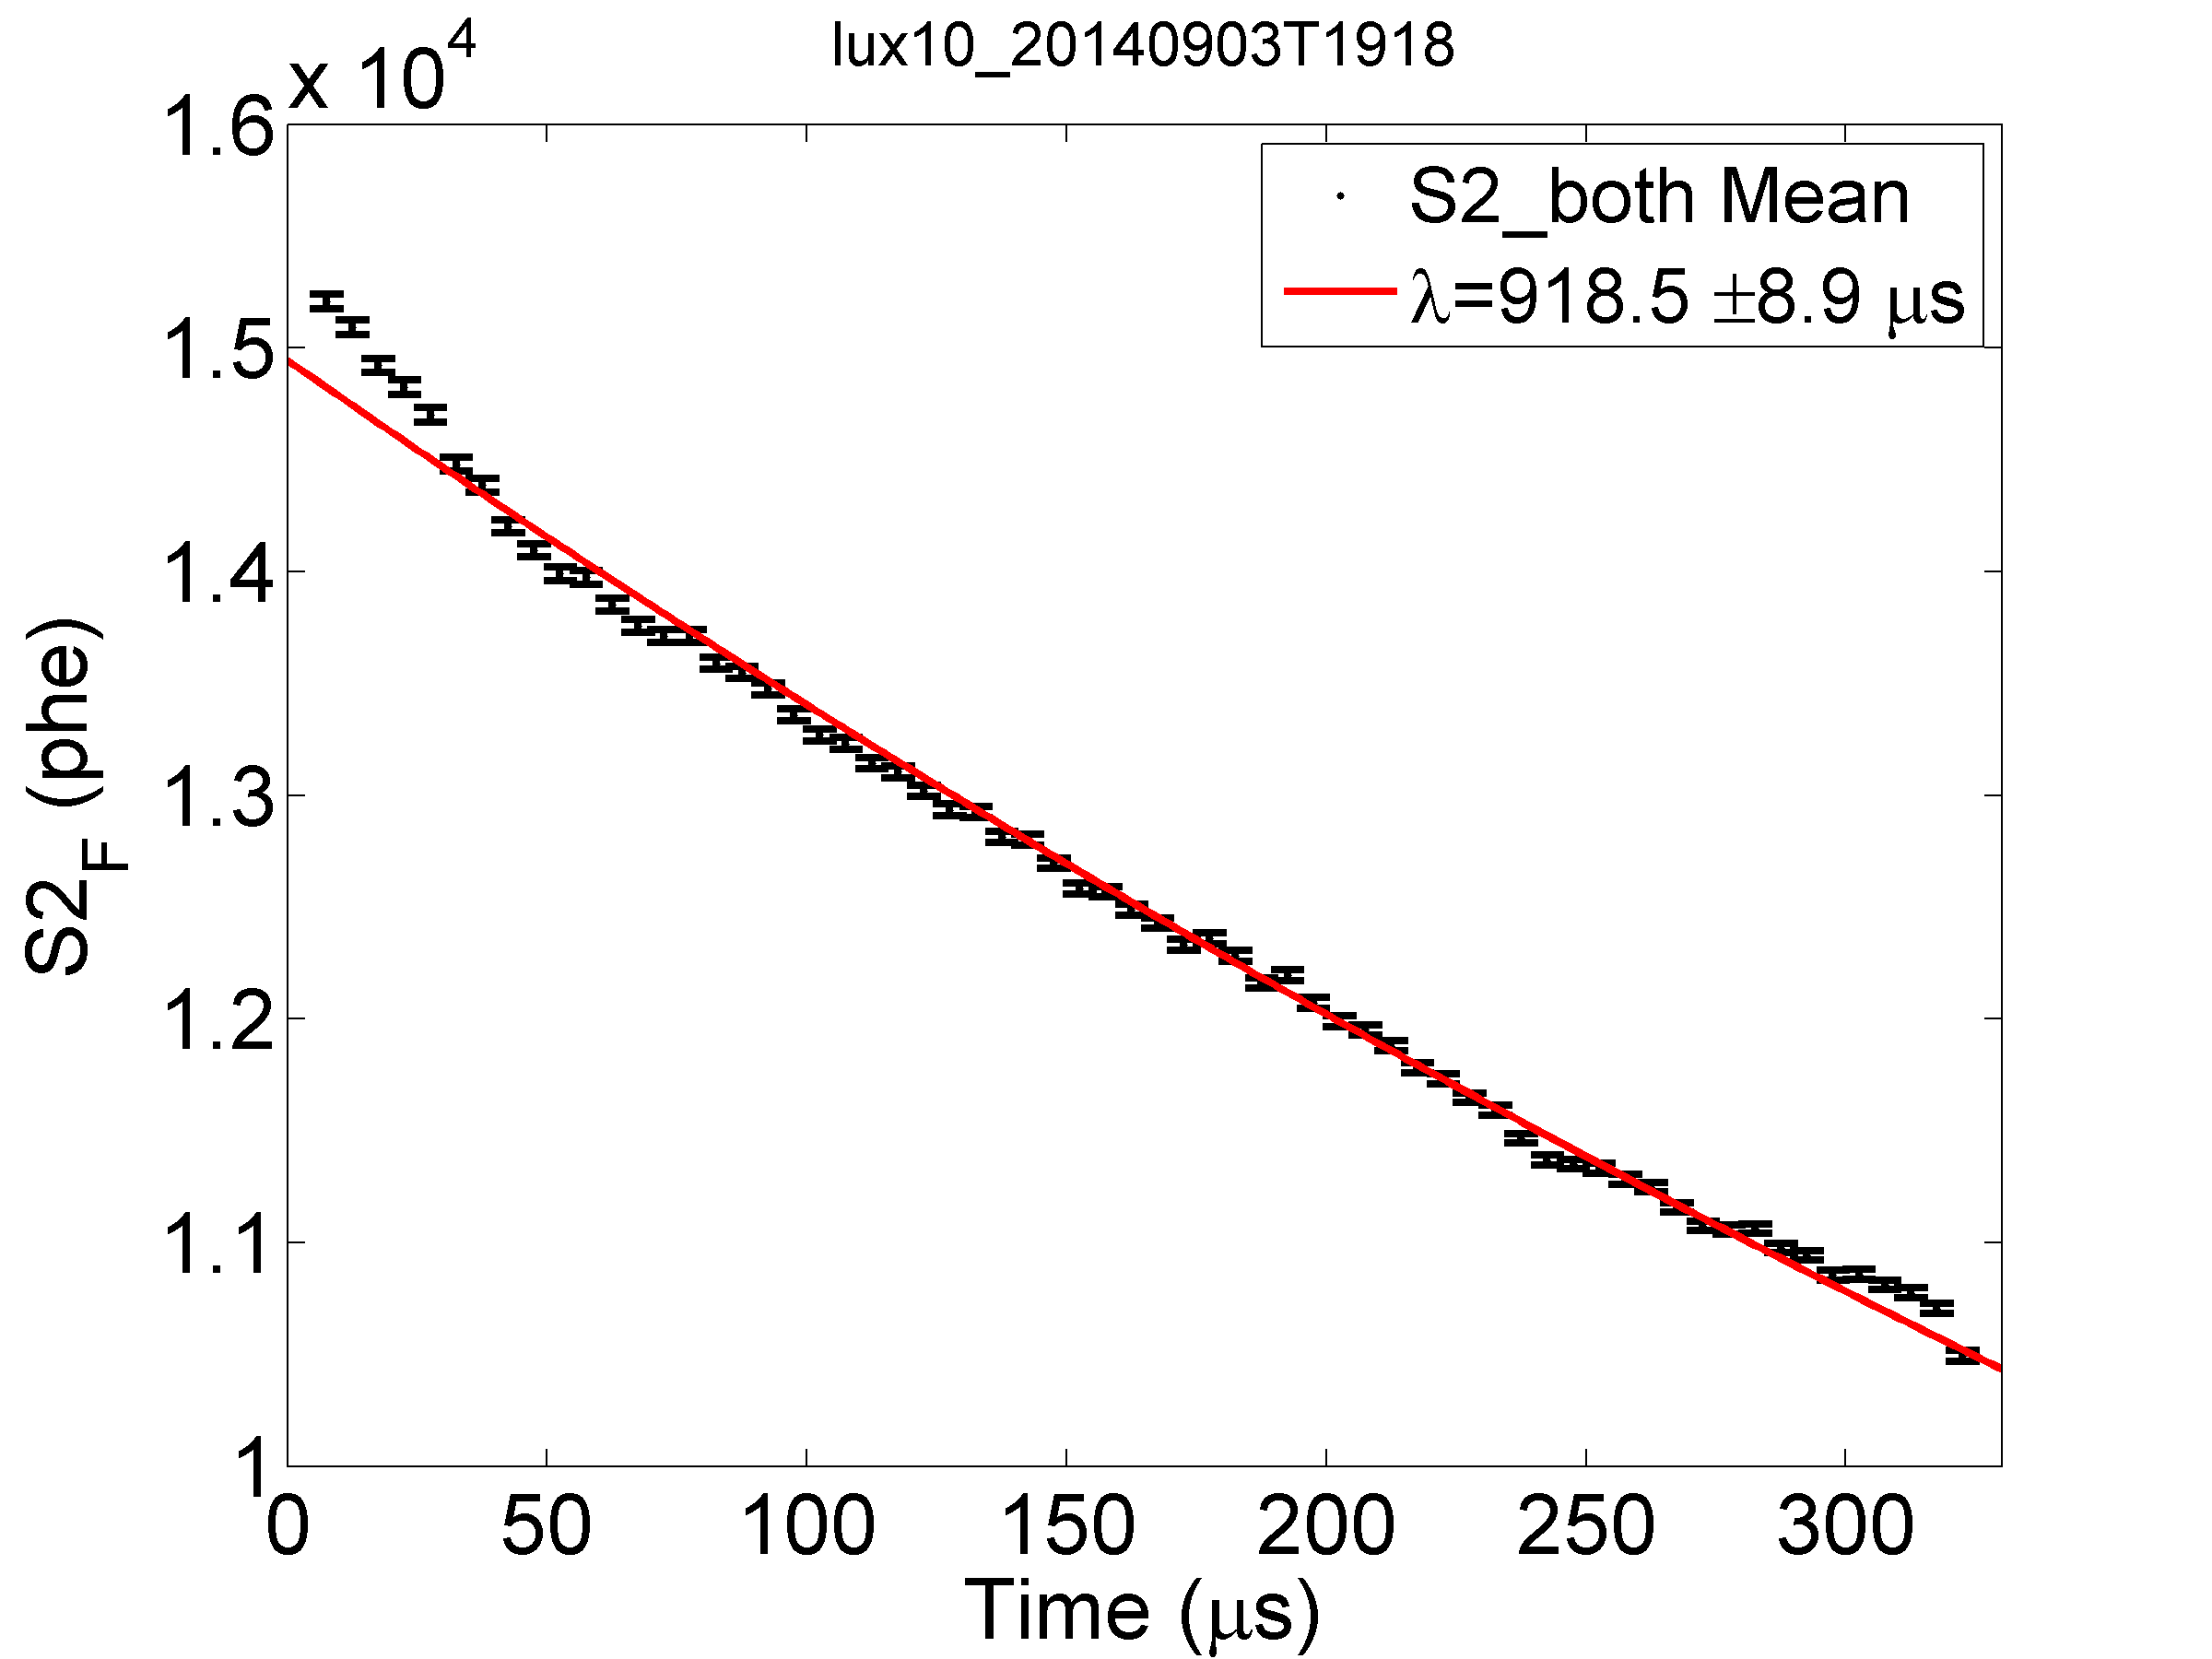
\includegraphics[width=6.5cm]{Run04Corrections/GoodLifetimeFit.png} }}
\qquad
\subfloat{{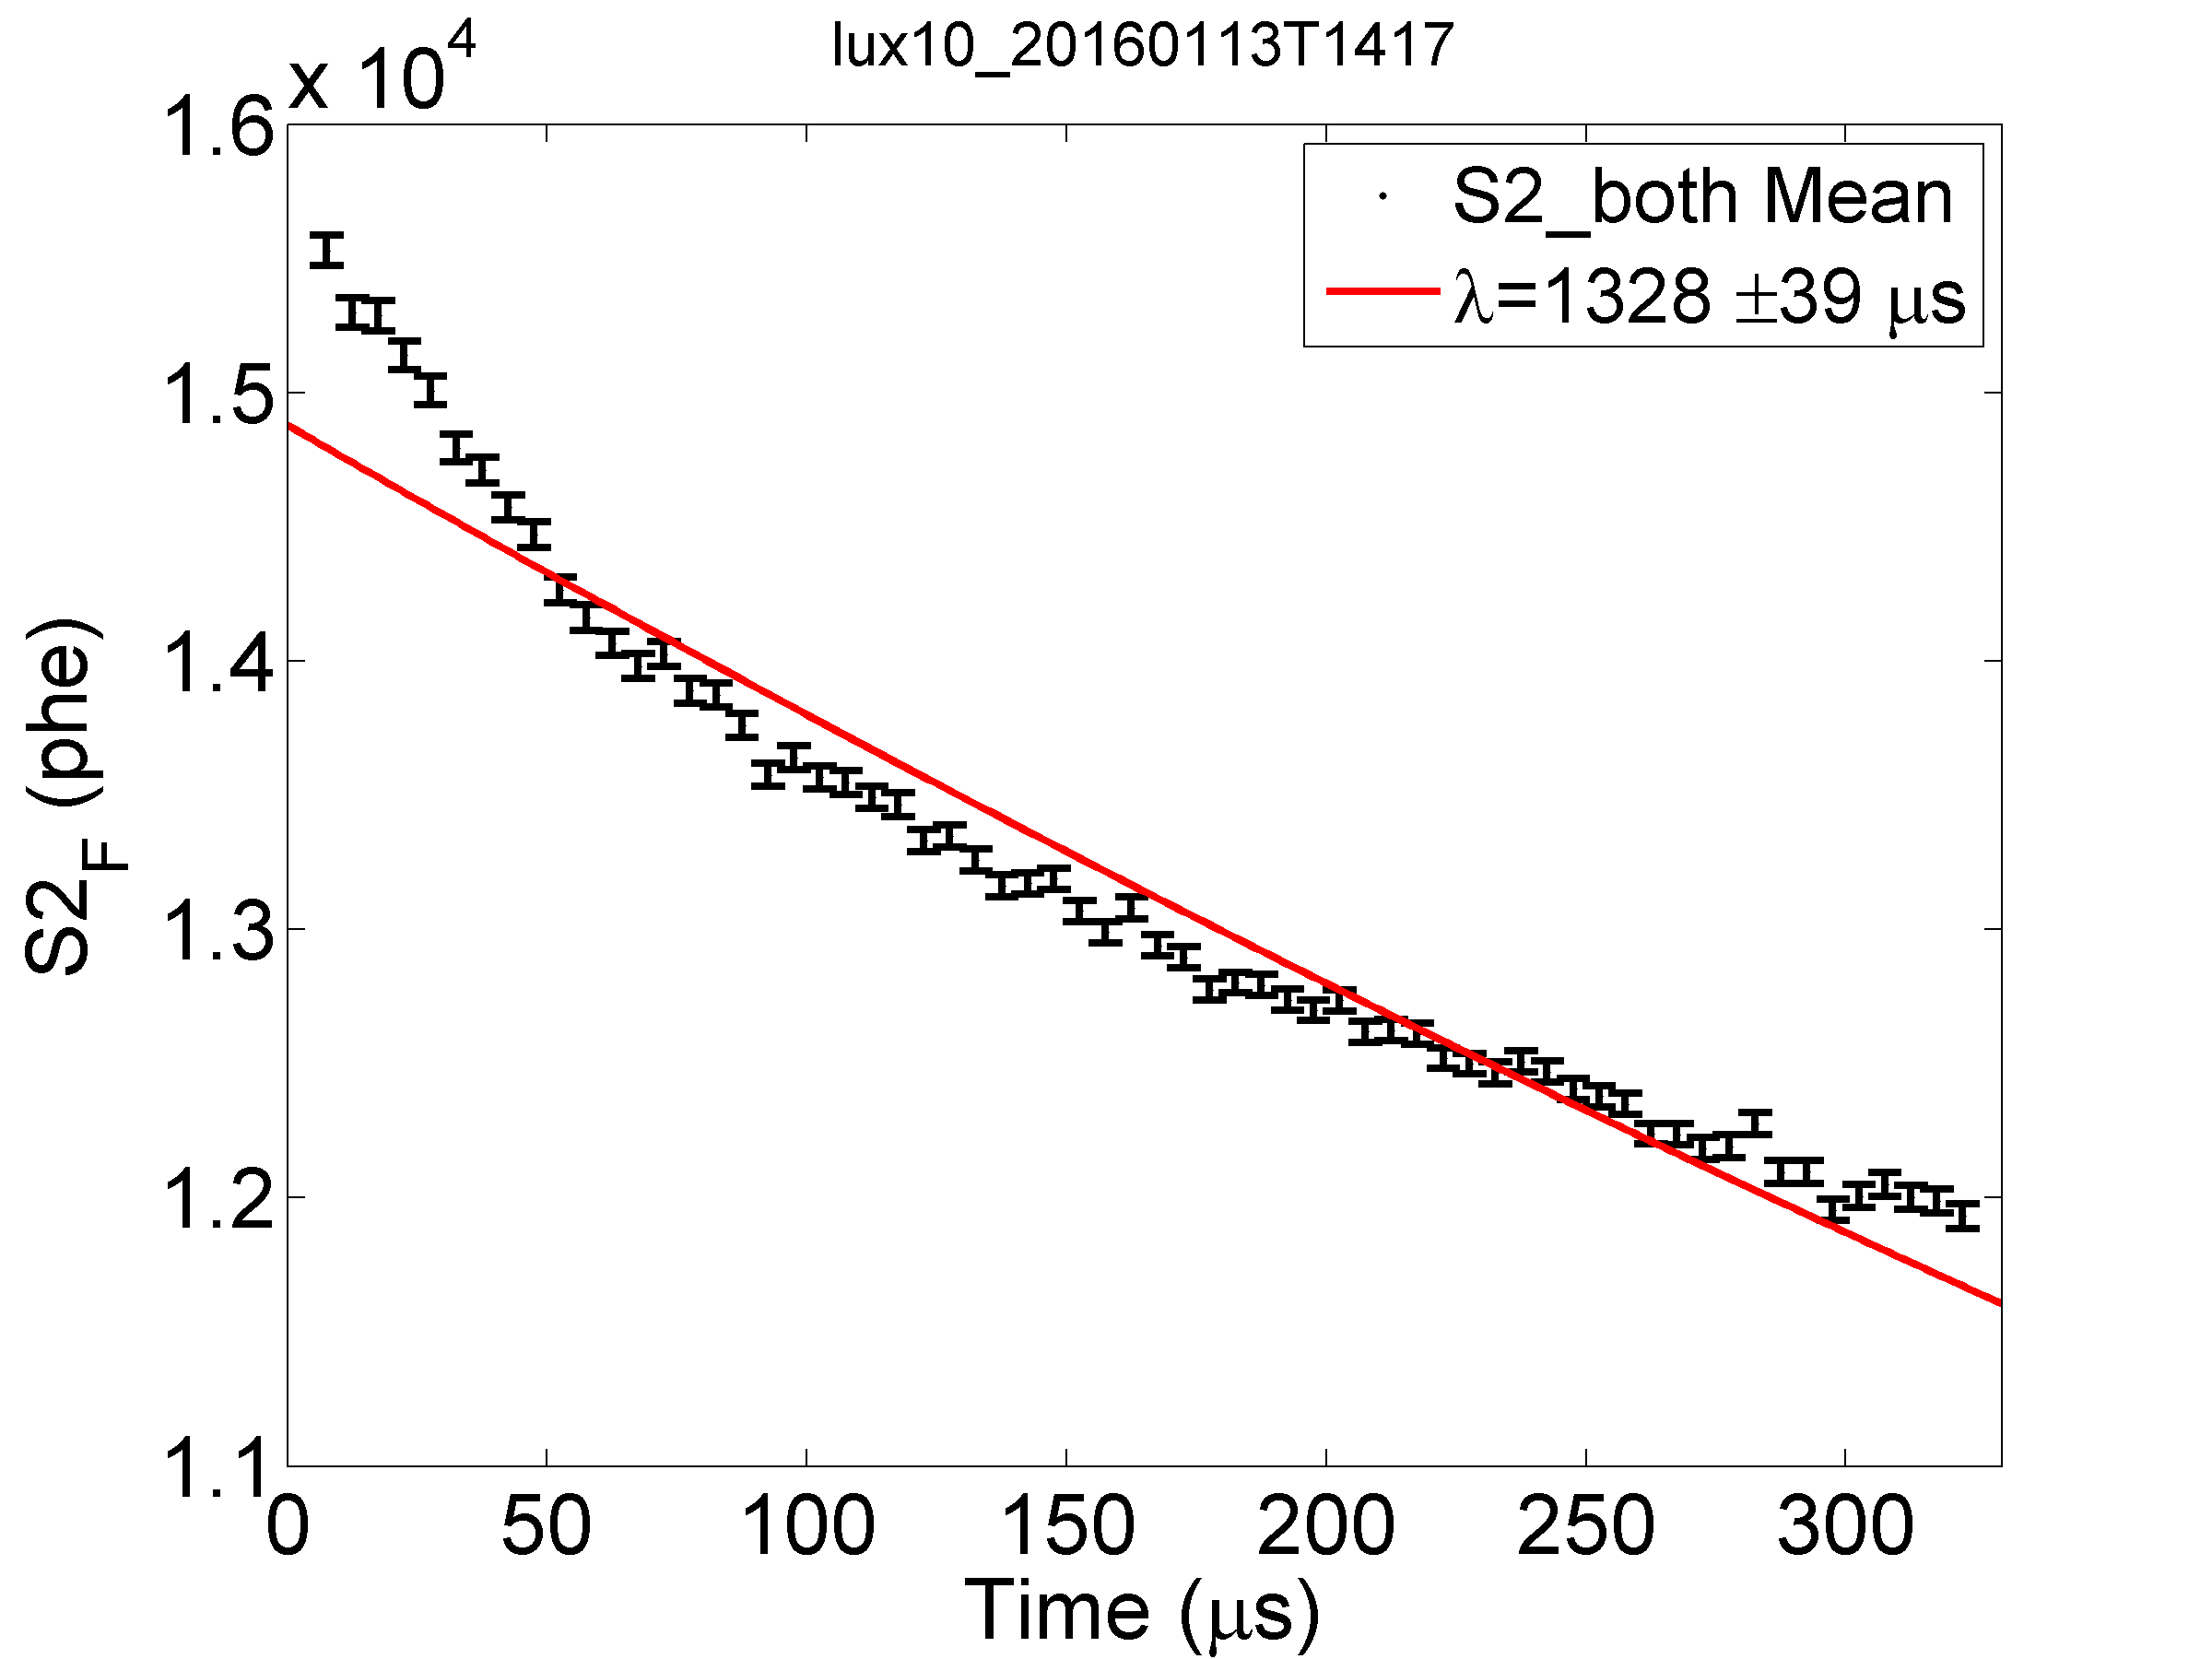
\includegraphics[width=6.5cm]{Run04Corrections/BadLifetimeFit.png} }}
\captionof{figure}{ (Left) A reasonable exponential fit to the S2$_F$ Z dependence in September 2014 (Right) A poor exponential fit to the S2$_F$ Z dependence in January 2016.  The higher field variation leads to a worse fit due to the drift velocity dependence of the absorption cross section.}
\label{ELFits}
\end{figure}




\begin{figure}[!h]
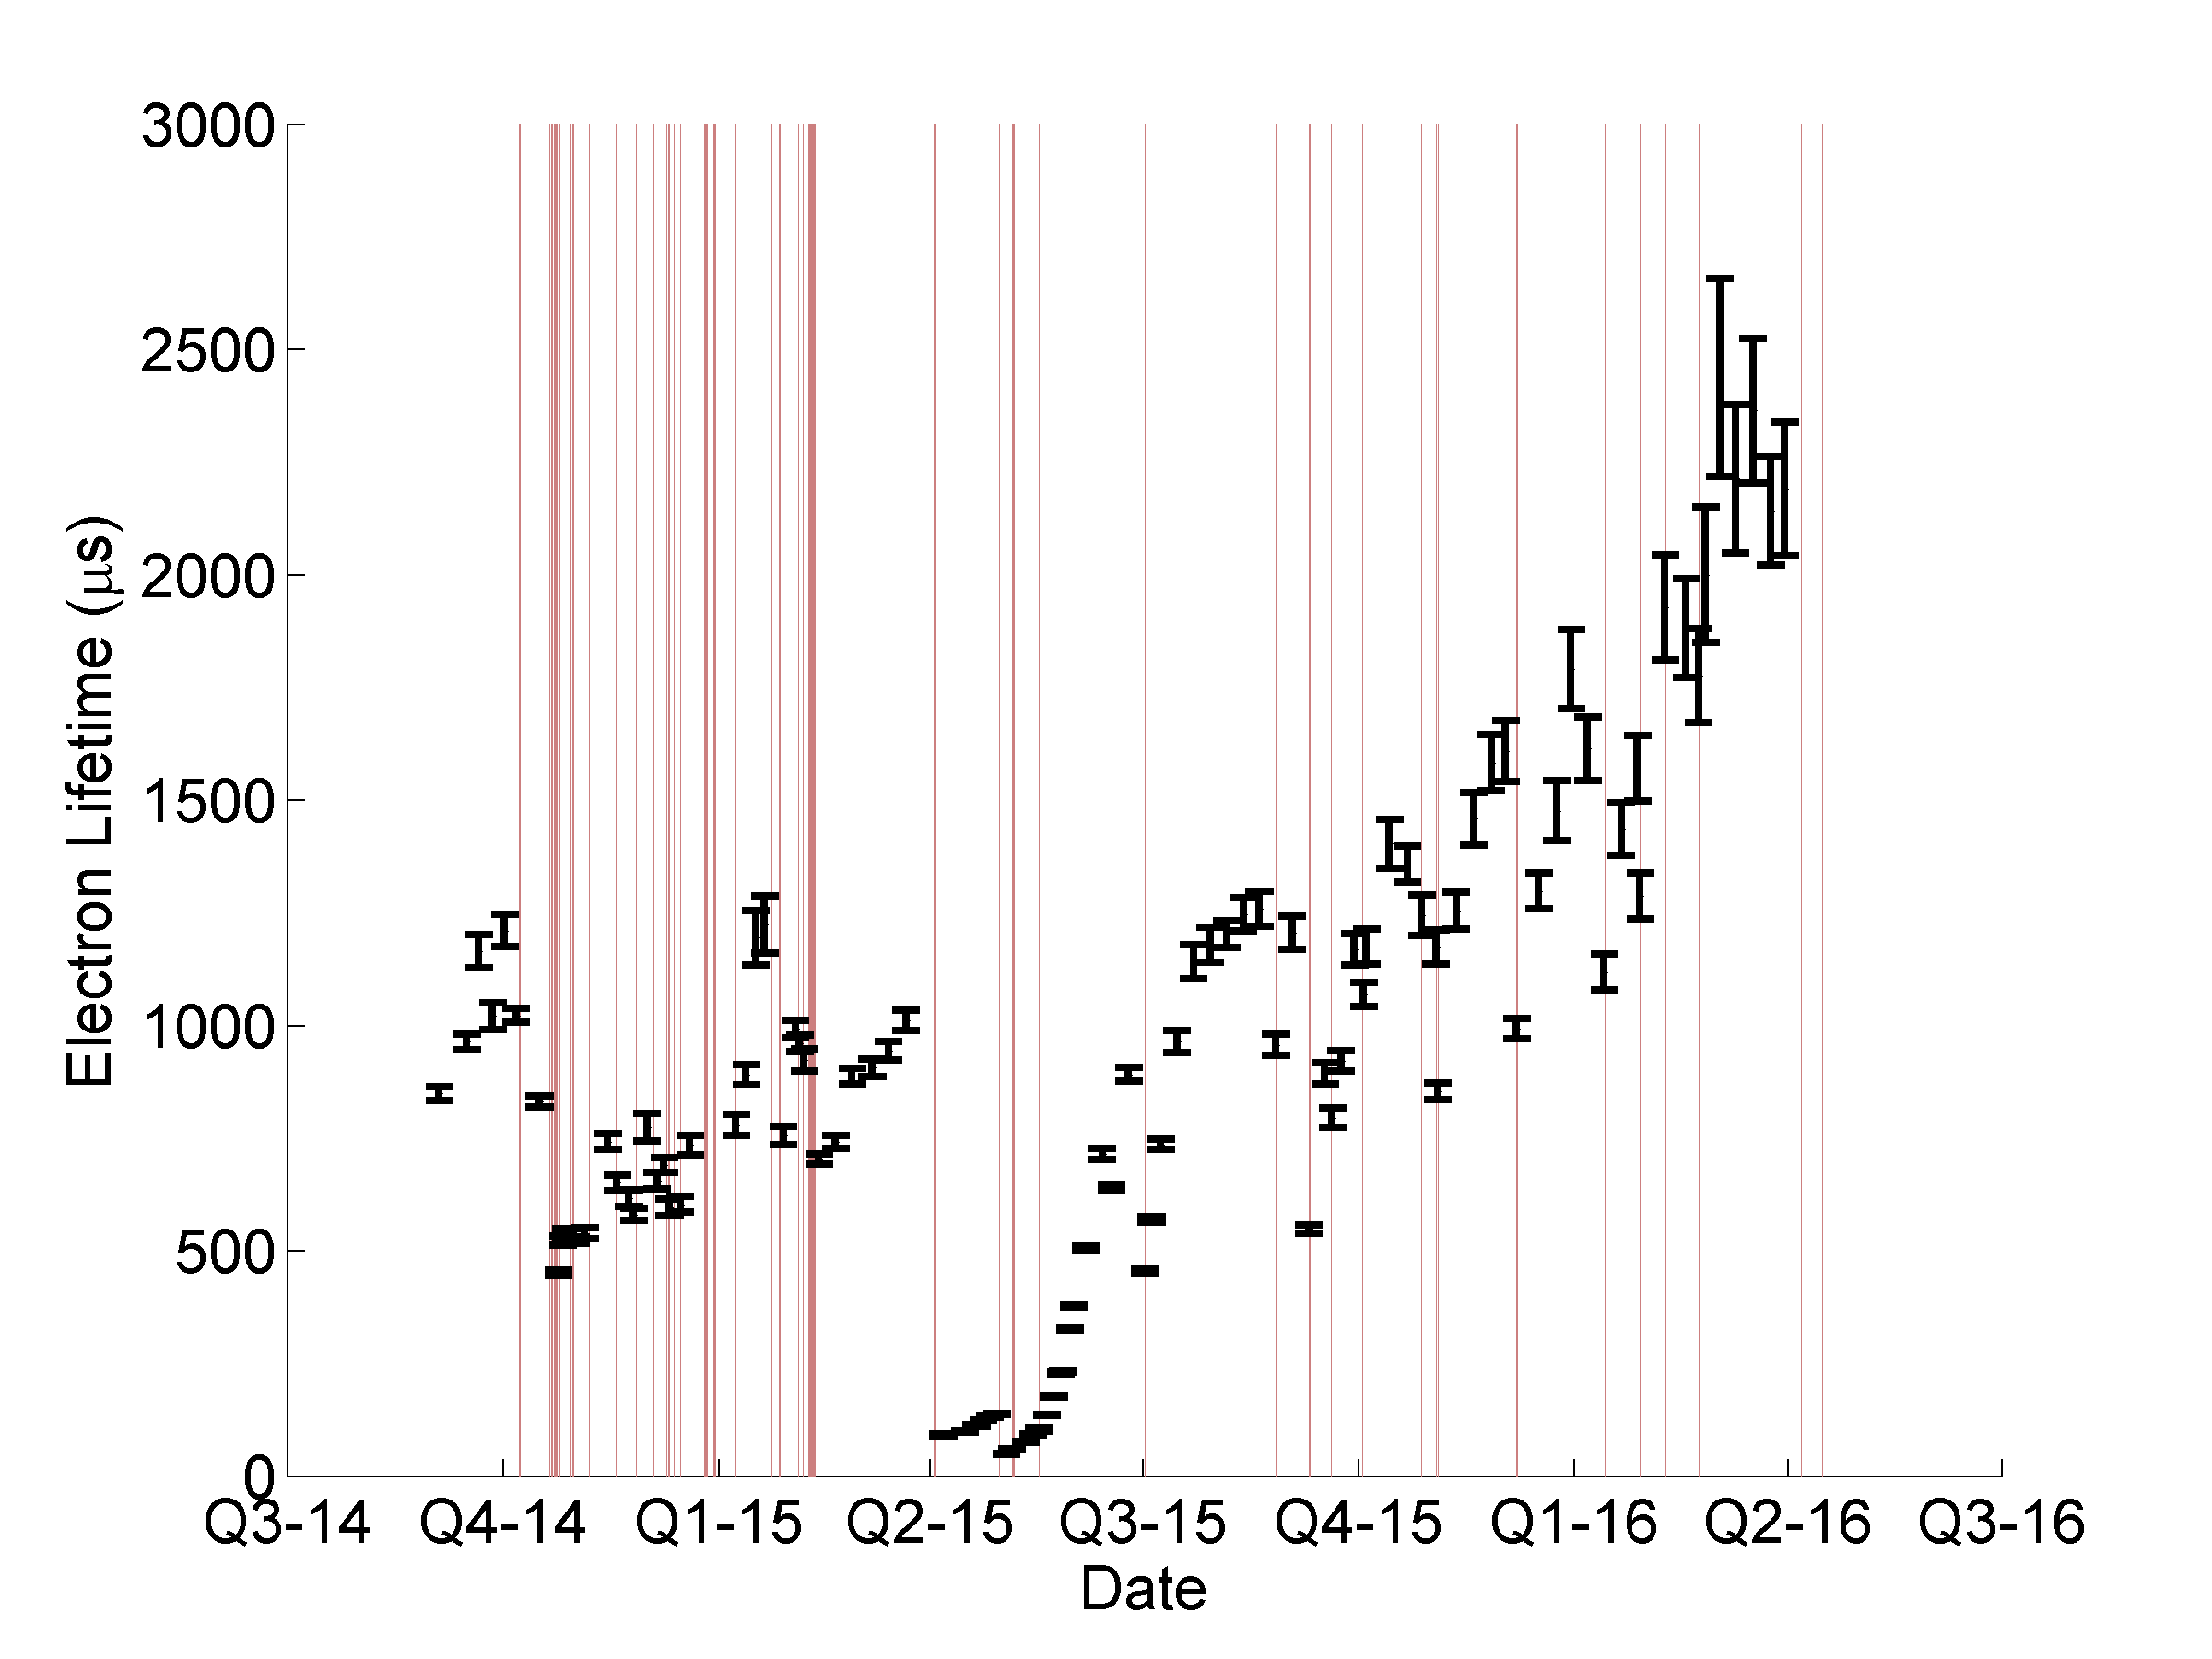
\includegraphics[scale=0.5]{Run04Corrections/LUX_eLifetime_Kr2p22.png}
\captionof{figure}{The electron lifetime over Run4 found by fitting an exponential to the S2$_F$ Z dependence.  Red areas indicate circulation outages.  At high lifetimes the S2$_F$ Z dependence is less exponential, and the small fraction of electrons that are lost is harder to measure, leading to larger errors on the measurement.}
 \label{fig:Run4Lifetime}
\end{figure}


\subsubsection{Additional Output from the Corrections Module: Single Electron Size}

Changes in the detector pressure, temperature, and liquid levels can cause the single electron size in the detector to vary over time.  These variations introduce variations in the size of $g_2$, so it is necessary to track the single electron size in each $^{83m}$Kr calibration data set.  In particular, we are interested in the single electron size at the center of the detector, since the field effects do not impact the result and the detector inefficiency effects are normalized to the center. 

We select a population of clean events by requiring 100 samples between the first S1 of a $^{83m}$Kr event and the single electron associated with it.  We then take two approaches to measure the single electron size at the center of the detector.  In the first approach, we measure the single electron size by fitting a skew Gaussian distribution to the single electron pulse area spectrum within the radius at which the single electron size begins to decay at the edges of the detector. (Figure \ref{SESize1}) In Run4, this radial limit is r$<$17 cm. In the second approach, we slice the detector into XY bins with widths determined such that each bin has roughly 100 single electron events.  A skew Gaussian distribution is fit to the single electron spectrum of each bin, and a XY map of the single electron size is constructed.  The value of the single electron size at the center of the detector is found with a spline interpolation of the XY dependence map.  (Figure \ref{SESize2})  These two methods agree within 1\%.

\begin{figure}[!h]
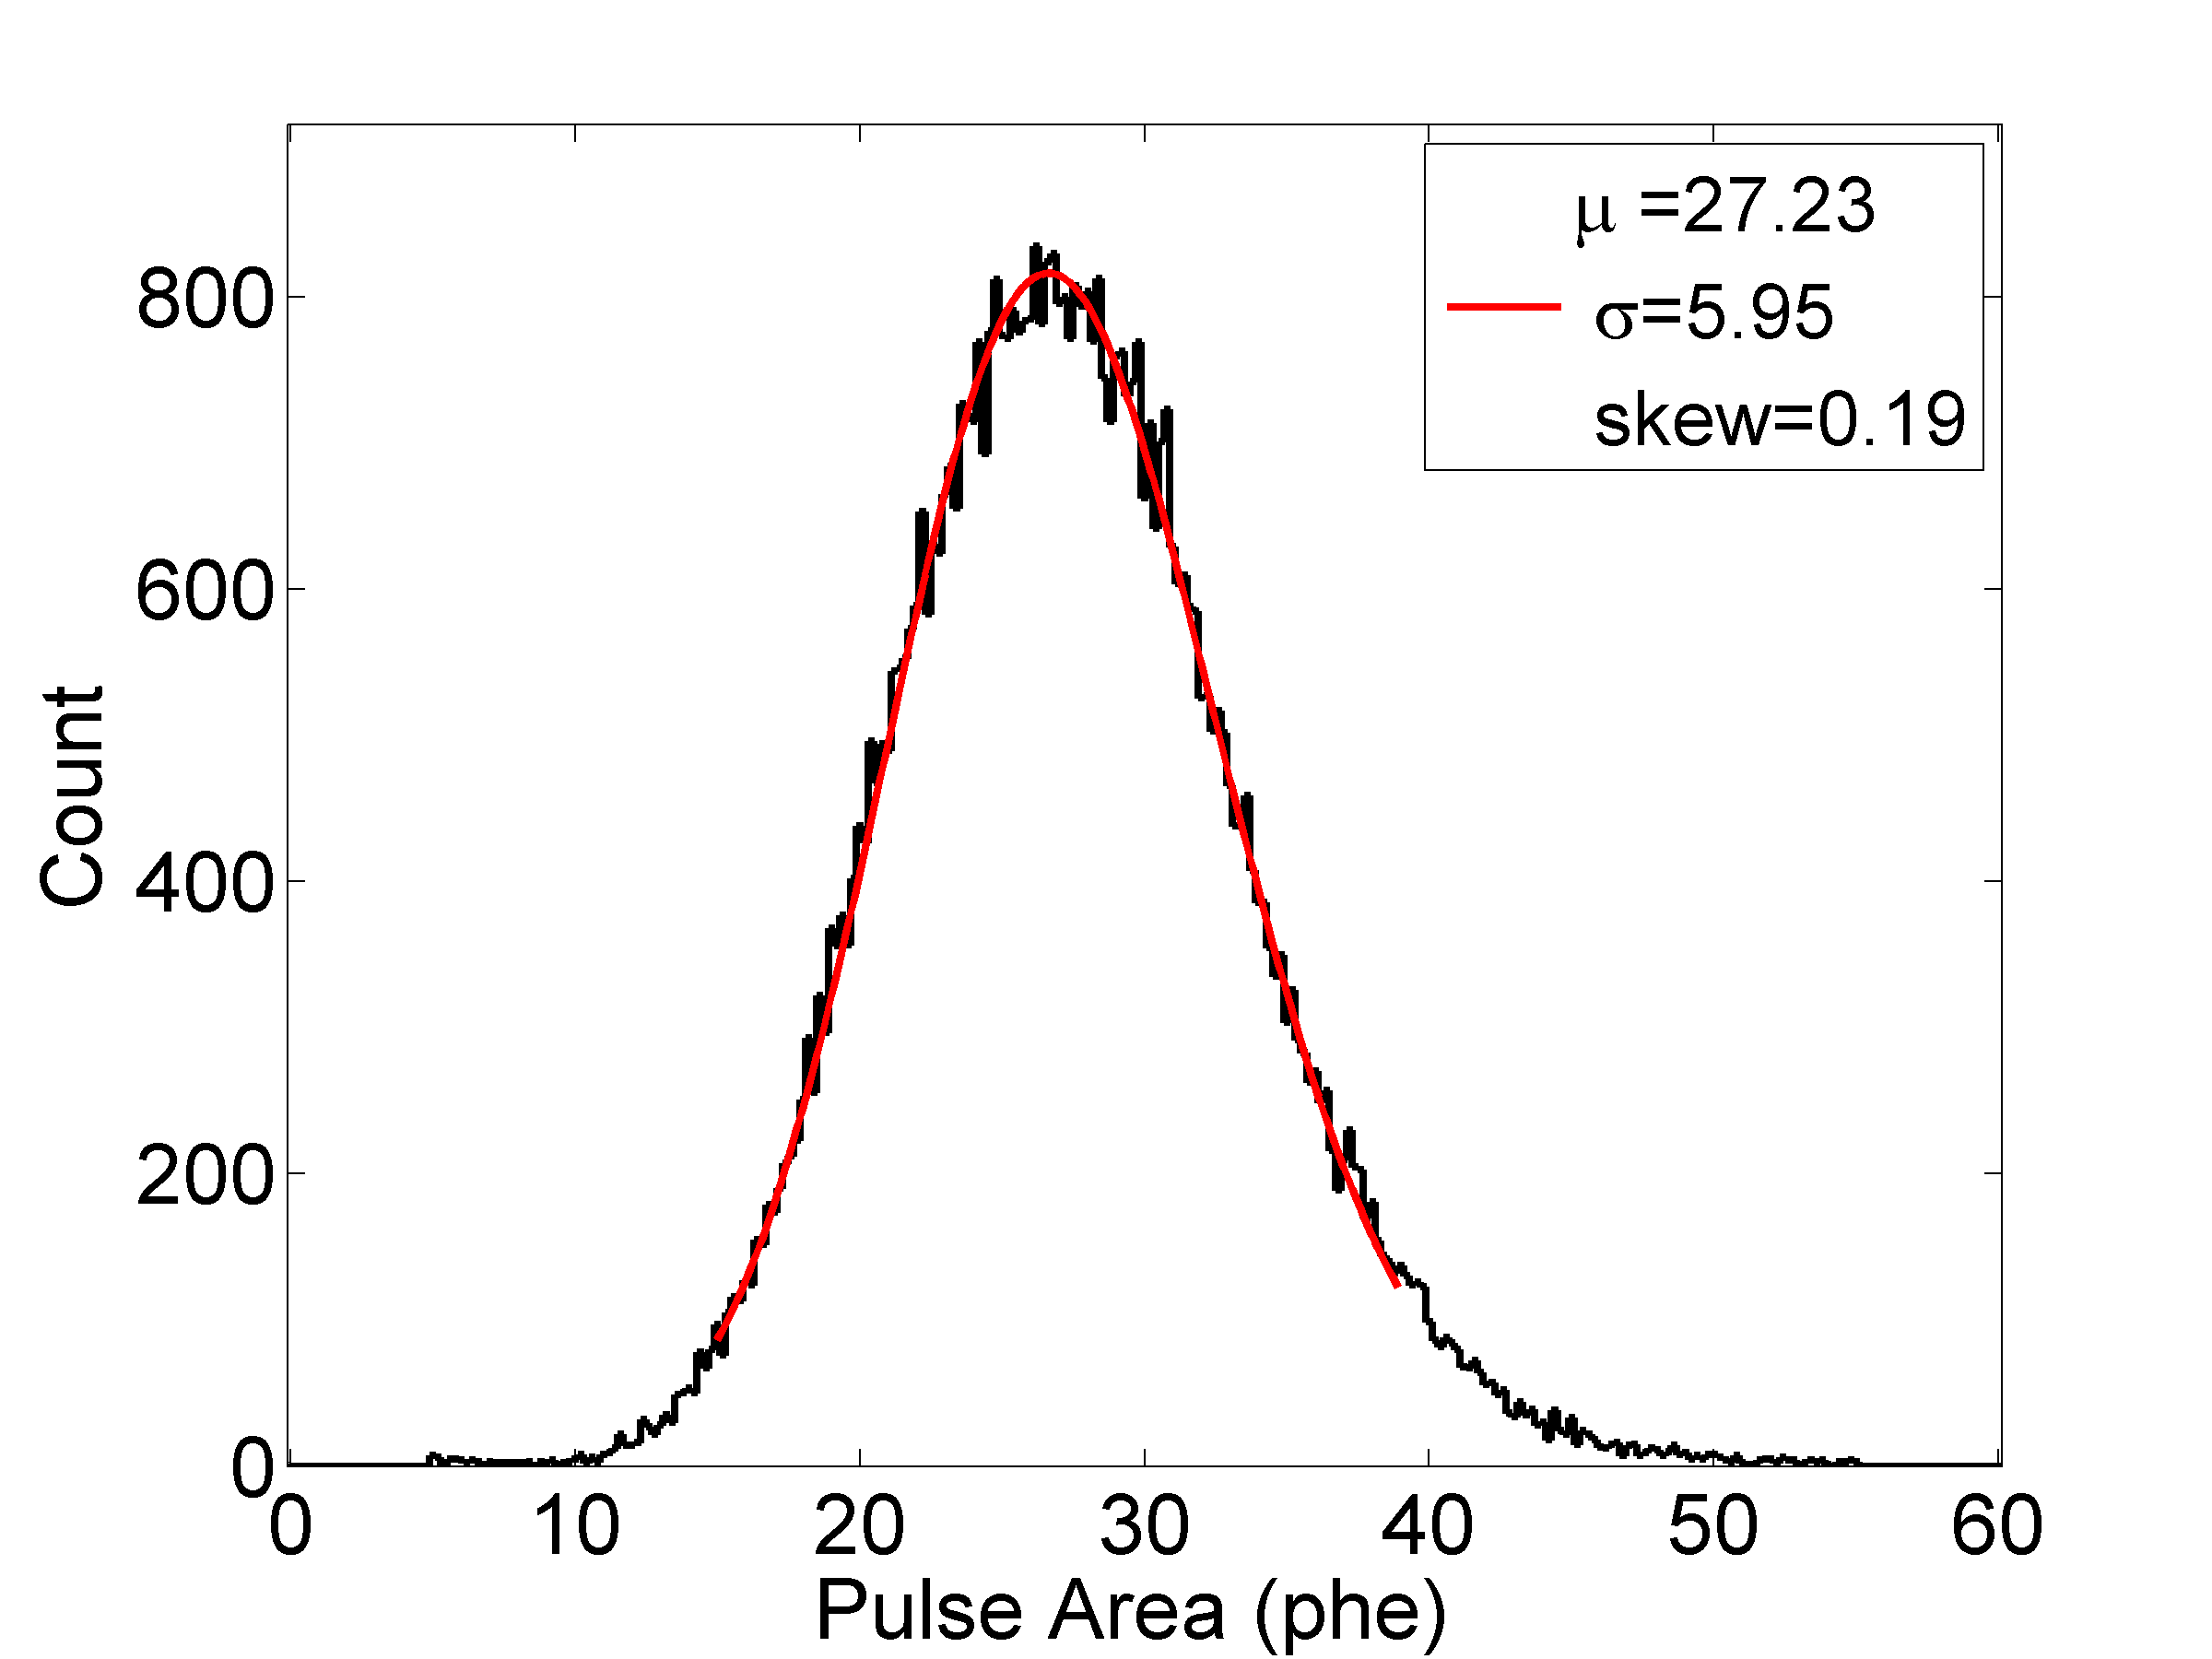
\includegraphics[scale=0.5]{Run04Corrections/SESizeExample.png}
\captionof{figure}{The result of our first approach for measuring the single electron size at the center of the detector.  We perform this measurement for every $^{83m}$Kr data set.  In this particular example from September 03, 2014 the single electron size is found to be 27.23 $\pm$ 0.044.}
 \label{SESize1}
\end{figure}

\begin{figure}[!h]
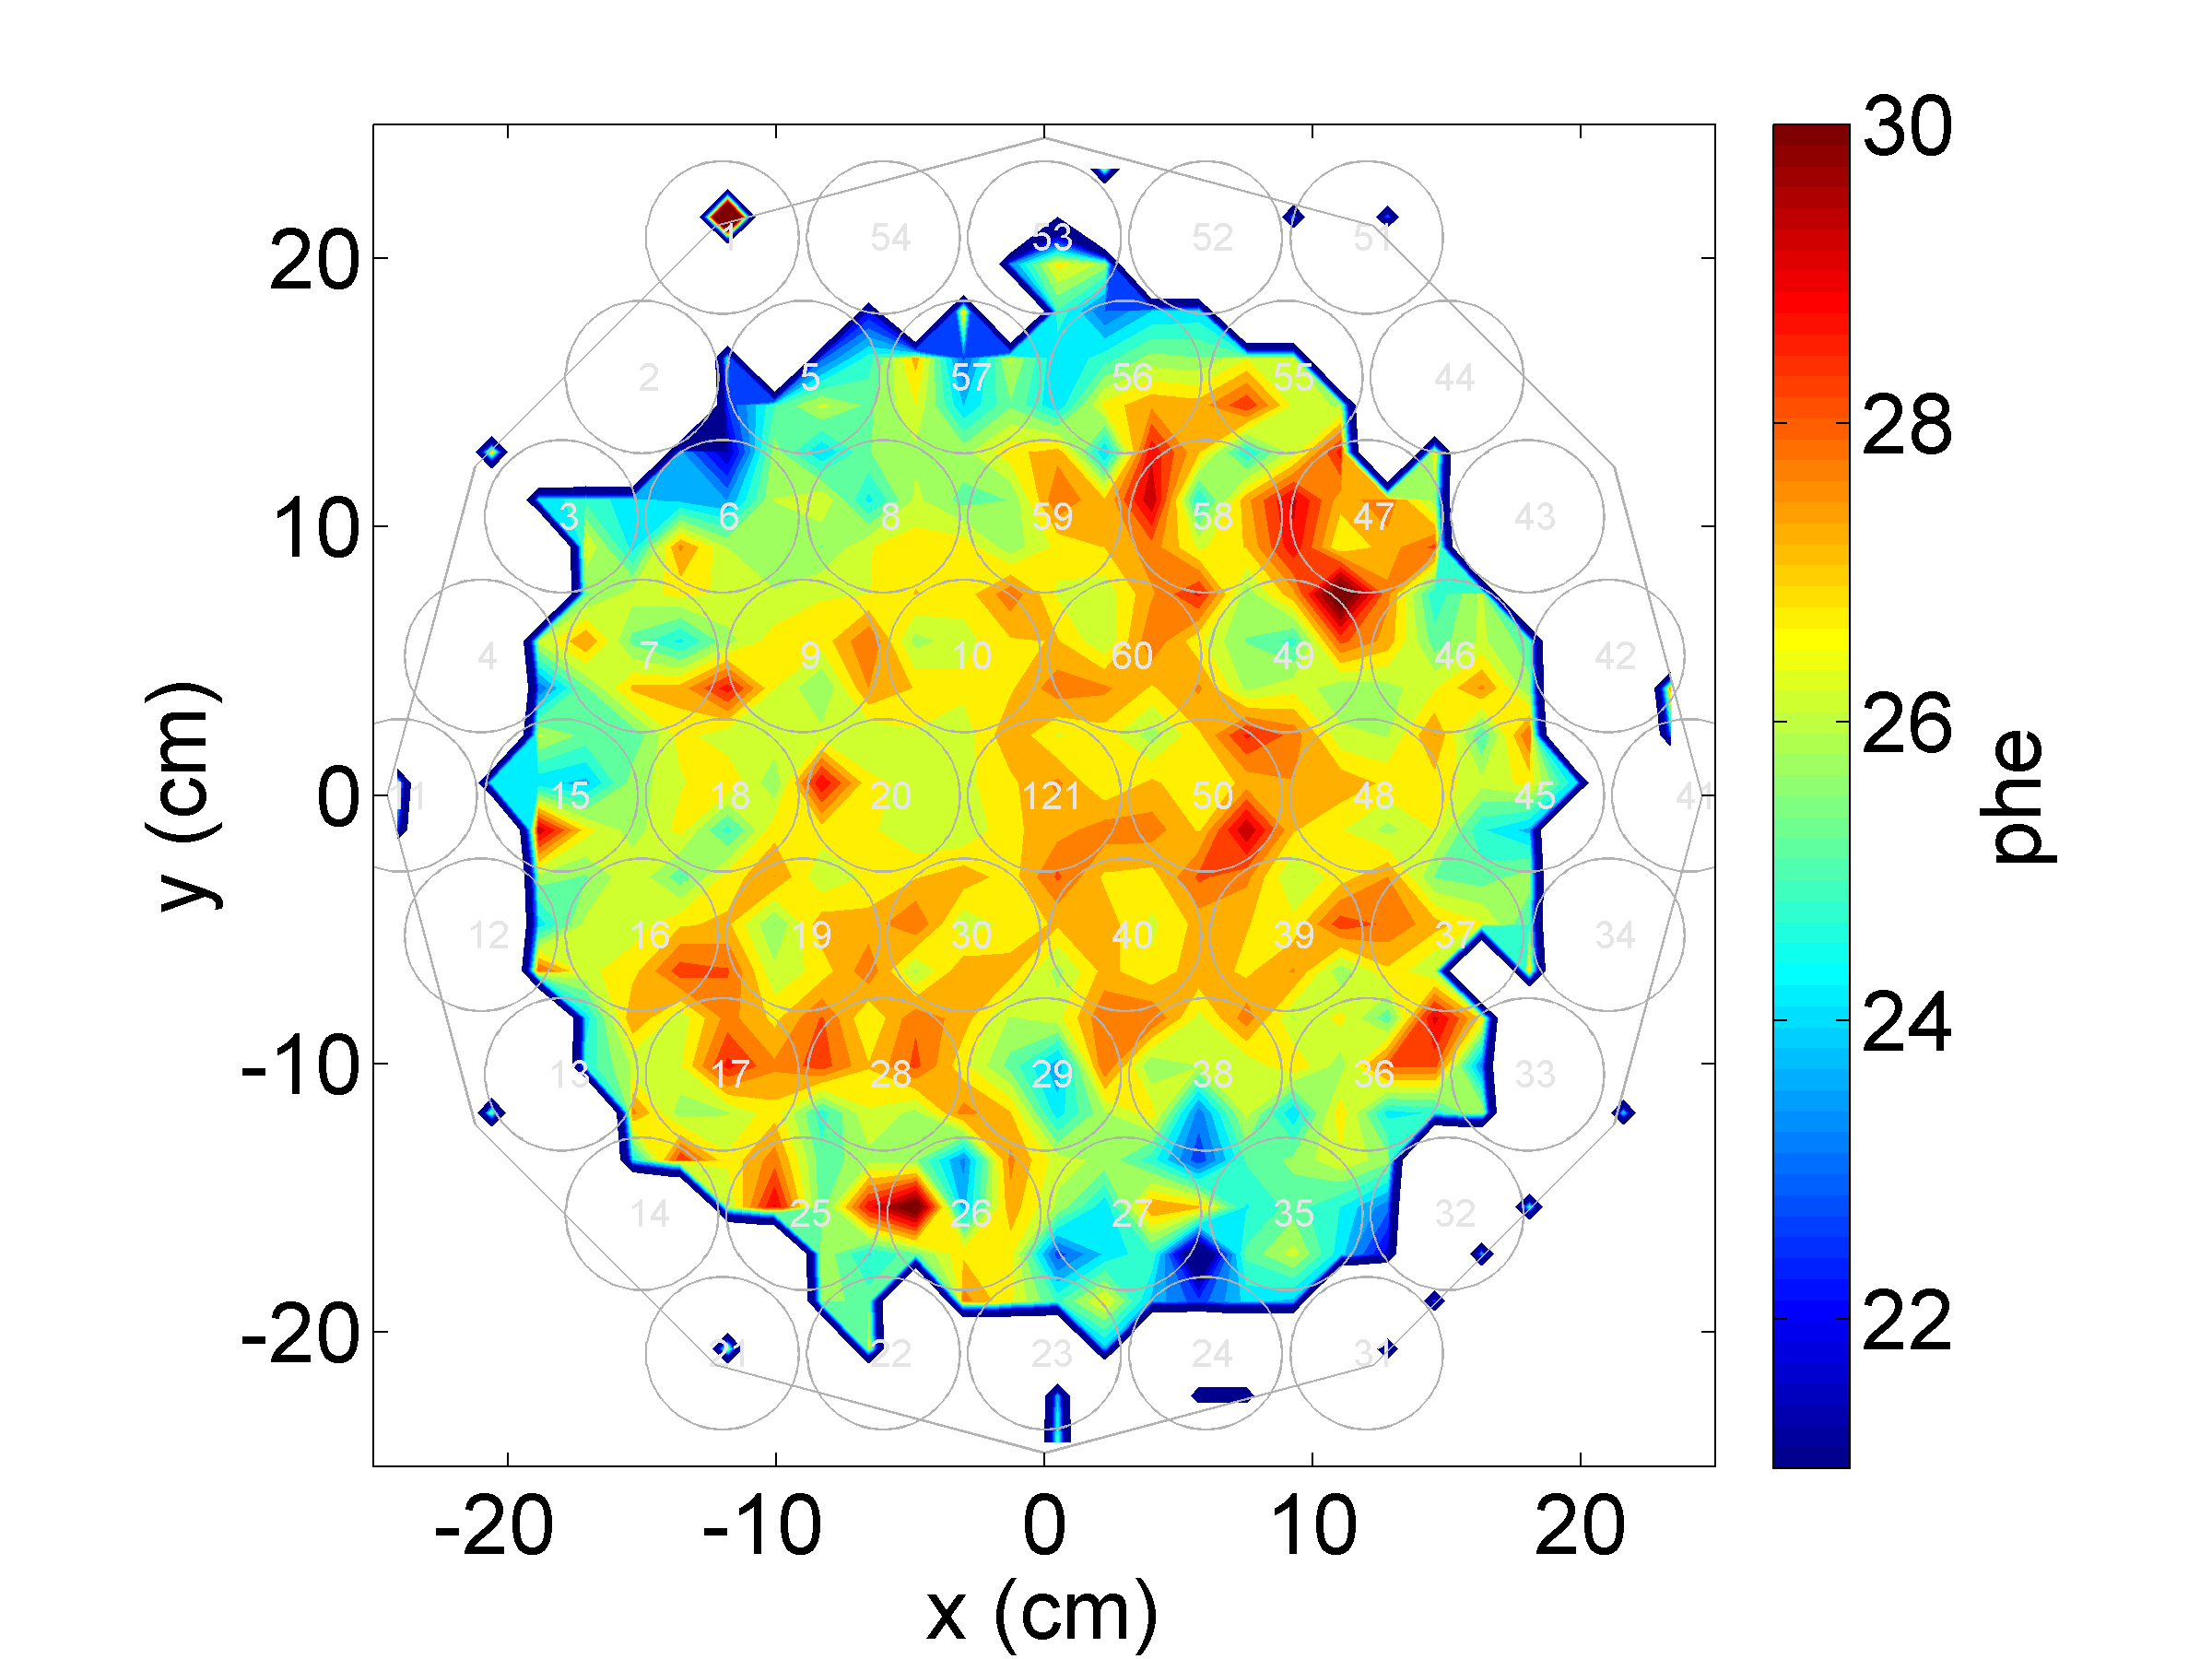
\includegraphics[scale=0.5]{Run04Corrections/SEXYSizeExample.png}
\captionof{figure}{The XY dependence of the single electron size used in our second approach for measuring the single electron size at the center of the detector.  We perform this measurement for every $^{83m}$Kr data set.  In this particular example from September 03, 2014 the single electron size is found to be 27.40 $\pm$ 0.31.}
 \label{SESize2}
\end{figure}

\subsubsection{Additional Output from the Corrections Module: Electric Field Maps}

Due to the time variation of the electric field in Run4 it is clearly important to measure the electric field in each $^{83m}$Kr calibration data set.  To accomplish this, we relate the RvZ field maps in September 2014 and September 2015 to the RvZ dependence of the S1a/S1b ratio during the same points in time (Figure \ref{FieldToS1aS1b}). In September 2014, the best fit polynomial for this relation is
\begin{equation}
\text{Field (V/cm)} =    (711 \pm 100) \left(\frac{S1a}{S1b} \right)^2 + (-4788 \pm 530) \left(\frac{S1a}{S1b} \right) + (7948 \pm 704)
\end{equation}
In September 2015, the best fit polynomial for this relation is
\begin{equation}
\text{Field (V/cm)} =    (1169 \pm 120) \left(\frac{S1a}{S1b} \right)^2 + (-7128 \pm 631) \left(\frac{S1a}{S1b} \right) + (10900 \pm 824)
\end{equation}
Although the measured S1a/S1b to electric field relationship is similar between the two datasets, the estimate of the field differs depending on which relationship is used.  We choose to use the average result of the two relationships for the reported field strength, and take the difference between them as a systematic error. (Figure \ref{KrypFieldMap}

\begin{figure}[!h]
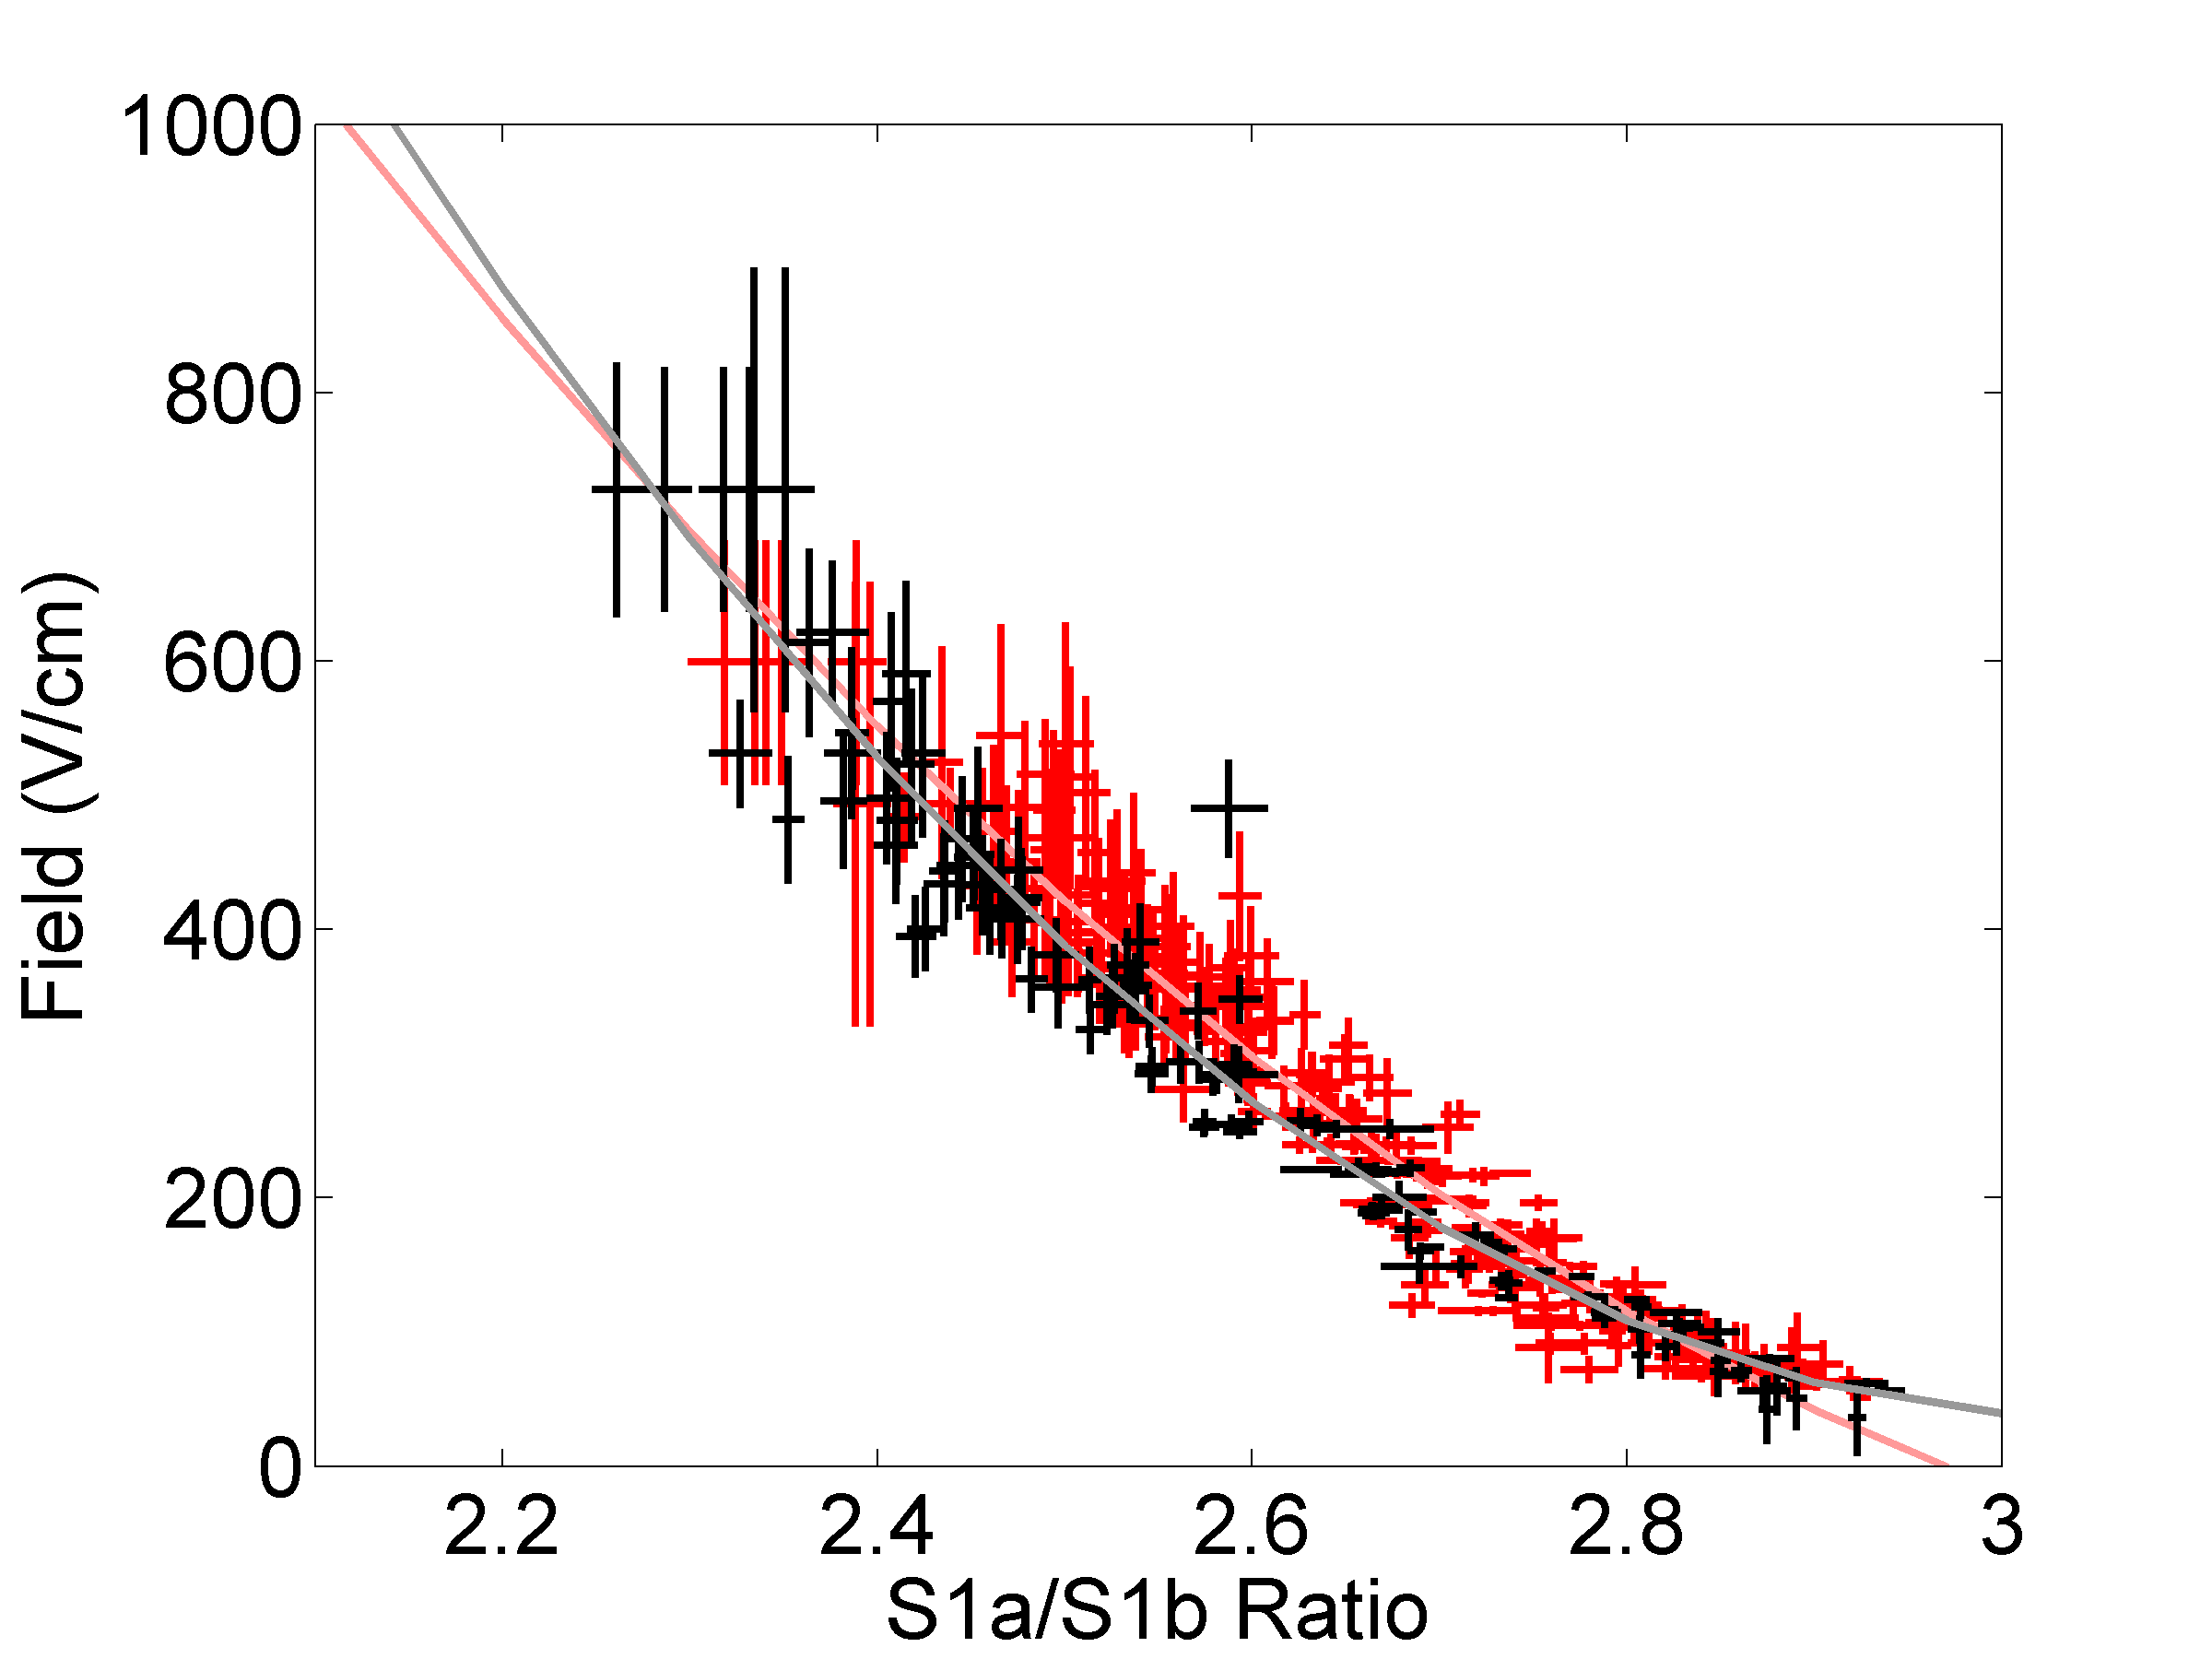
\includegraphics[scale=0.6]{Run04Corrections/S1aS1bToField_Overlay.png}
\captionof{figure}{The S1a/S1b to field strength relationship measured in September 2014 (red) and September 2015 (black). }
 \label{FieldToS1aS1b}
\end{figure}

\begin{figure} [!h]
\centering
\subfloat{{\includegraphics[width=6.5cm]{Run04Corrections/KrypCalFieldMap.png} }}
\qquad
\subfloat{{\includegraphics[width=6.5cm]{Run04Corrections/KrypCalFieldMapError.png} }}
\captionof{figure}{ (Left) R$^2$vZ map of the electric field on September 03, 2014 as measured by KrypCal (Right) R$^2$vZ map of the systematic error in the electric field measurement on September 03, 2014.}
\label{KrypFieldMap}
\end{figure}

%Add s2 width section for thesis, and describe each of these subsections in more detail at that time

\subsection{Results of the KrypCal Corrections} \label{Results}

In this section we will cover a number of metrics which have been used to determine how well the KrypCal corrections are working in Run4.  A version of KrypCal which does not acknowledge the spatial and time dependent field in Run4 (similar to what we did in Run3) has been produced for comparison of each metric.


\subsubsection{Energy Spectra}\label{Result:Spectra}

The $\chi^2$ method presented in section \ref{section:S1relation2} finds an average total reduced $\chi^2$ of 0.8413 for the CH$_3$T and $^{83m}$Kr energy spectra, with a reduced $\chi^2$ of  150.6/124=1.2143 (p=0.05) for CH$_3$T alone and a reduced $\chi^2$ of 12.17/26=0.4682 (p=0.99) for $^{83m}$Kr alone.  The resulting $^{83m}$Kr energy spectra (unbinned in drift time) from September 2015 and February 2016 are shown in figure \ref{Kr2p22_KrE}.  The Gaussian means differ from the expected 41.55 keV by less than one sigma, and the reduced $\chi^2$ based on the Z dependence of the Energy spectra returns a p-value of 0.99.

\begin{figure} [!h]
\centering
\subfloat{{\includegraphics[width=6.5cm]{Run04Corrections/KrEnergy.png} }}
\qquad
\subfloat{{\includegraphics[width=6.5cm]{Run04Corrections/KrEnergyZDep.png} }}
\captionof{figure}{ (Left) The energy spectrum of $^{83m}$Kr data in September 2014 (red) and September 2015(blue) after determining the S1 field effect to S1a/S1b relationship from the  reduced $\chi^2$ method. The energy spectrum is expected to be a Gaussian distribution centered around the black line.  (Right) The Z dependence of the $^{83m}$Kr energy peaks in September 2014 (red) and September 2015 (black).}
\label{Kr2p22_KrE}
\end{figure}

The CH$_3$T energy spectra from calibrations in September 2014, November 2014, February 2015, September 2015, and February 2016 are shown in figure \ref{Kr2p22_H3E}.  The fractional difference between the expected CH$_3$T spectrum and the CH$_3$T is shown below each energy spectrum.  Fractional residuals of up to 3 $\sigma$ are comparable to our CH$_3$T results from Run3.


\begin{figure} [!h]
\includegraphics[scale=0.7]{Run04Corrections/KrypCal_2p22_AllCH3TEnergy.png}
\captionof{figure}{The September 2014, November 2014, February 2015, September 2015, and February 2016 CH$_3$T energy spectra resulting from KrypCal corrections.  The bottom panels show the fractional residuals.}
 \label{Kr2p22_H3E}
\end{figure}


A version of $^{83m}$Kr which does not acknowledge the spatial and time dependent field in Run4 produces the $^{83m}$Kr energy spectra shown in Figure \ref{BadKrypCalKr} and the CH$_3$T energy spectra shown in Figure \ref{BadKrypCalH3}.  This version of KrypCal produces corrections that normalize the $^{83m}$Kr S1 and S2 signals everywhere in the detector, regardless of whether the variation is induced by field effects or detector inefficiency. An optimal value of $g_1=0.100 \pm 0.001$ and extraction efficiency of EE$=1.08 \pm 0.030$ is found by an energy spectrum $\chi^2$ fit.  This optimal value of the extraction efficiency is 40\%-80\% higher than our expectations based on Guschin data and our extraction field strength, and exceeds 100\%.  Even with the unreasonably high extraction efficiency, the $^{83m}$Kr and CH$_3$T energy spectra produce a worse average reduced $\chi^2$ of 1.12 for the $^{83m}$Kr and CH$_3$T energy spectra when compared to the expected energy spectra, with a reduced $\chi^2$ of 10.06/26=0.3869 for $^{83m}$Kr alone, and a reduced $\chi^2$ of 230.2/124=1.8562 for CH$_3$T alone.

\begin{figure} [!h]
\centering
\subfloat{{\includegraphics[width=6.5cm]{Run04Corrections/KrSpectraWithoutFieldCorrection.png} }}
\qquad
\subfloat{{\includegraphics[width=6.5cm]{Run04Corrections/KrSpectraZDepWithoutFieldCorrection.png} }}
\captionof{figure}{ (Left) The energy spectrum of $^{83m}$Kr data in February 2016 (red) and September 2015(blue) using a version of KrypCal that does not properly account for field effects. The energy spectrum is expected to be a Gaussian distribution centered around the black line.  (Right) The Z dependence of the $^{83m}$Kr energy peaks in September 2015 (red) and February 2016 (black) using the same version of KrypCal.}
\label{BadKrypCalKr}
\end{figure}


\begin{figure} [!h]
\centering
\subfloat{{\includegraphics[width=6.5cm]{Run04Corrections/TritumSpectrumWithoutFieldCorrection_Sep2015.png} }}
\qquad
\subfloat{{\includegraphics[width=6.5cm]{Run04Corrections/TritumSpectrumWithoutFieldCorrection_Feb2016.png} }}
\captionof{figure}{ (Left) The energy spectrum of CH$_3$T data in September 2015 (left) and February 2016 (right)  using a version of KrypCal that does not properly account for field effects.  The expected CH$_3$T energy spectrum for each data set is shown in black.}
\label{BadKrypCalH3}
\end{figure}



\subsubsection{Energy Threshold}

The Run4 energy threshold calculated by comparing the expected CH$_3$T energy spectrum to the measured CH$_3$T energy spectrum in September 2014, November 2014, February 2015, September 2015, and February 2016 is shown in Figure \ref{Thresholds}. The 50\% efficiency measurements are shown in Table \ref{ThreshTable}.  The average detector threshold of 1.19 $\pm$ 0.64 keV is consistent with libNEST expectation of 1.29 $\pm$ 0.17 keV, which was measured by comparison of the tritium beta spectrum input to the libNEST energy output.

\begin{center}
\begin{tabular}{| c | c |} 
\hline
Date & 50\% Threshold (keV)  \\ \hline \hline
September 2014 & 1.11  $\pm$ 1.07 \\ \hline
November 2014 & 1.17 $\pm$ 0.38  \\ \hline
February 2015 & 1.25 $\pm$ 0.23  \\ \hline
September 2015 & 1.22 $\pm$ 0.22  \\ \hline
February 2016 & 1.21 $\pm$ 0.52  \\ 
\hline
\end{tabular}
\captionof{table}{The energy threshold calculated from the CH$_3$T spectrum on different dates.}
\label{ThreshTable}
\end{center}

%Expected threshold comes from 
%https://ipython.nersc.gov/user/rknoche/notebooks/iPyNb/Analysis_Code/Run4_KrypCal2p22_NESTmodel/Sep2015_CH3T_Spectrum_Sim_Kr2p21.ipynb#

\begin{figure}[!h]
\includegraphics[scale=0.7]{Run04Corrections/KrypCal_2p22_Threshold.png}
\captionof{figure}{The September 2014, November 2014, February 2015, and September 2015 energy thresholds resulting from KrypCal corrections.}
 \label{Thresholds}
\end{figure}


\subsubsection{G1 and EE}

The $\chi^2$ method presented in section \ref{section:S1relation2} finds best fit values of $g_1=0.098 \pm 0.001$ and $EE=0.808 \pm 0.029$.  This is consistent with our expectations of an extraction efficiency between 0.6 and 0.8, based on our extraction field models and the Run4 liquid level, and is much better than the $g_1=0.100 \pm 0.001$ and $EE=1.08 \pm 0.030$ result found in section \ref{Result:Spectra}. (Figure \ref{EEexpec})  Likewise, the best fit value of $g_1$ is within one sigma of our expectation of g$_1$=0.108 $\pm$ 0.010 found in section \ref{G1pred}. 

\begin{figure}[!h]
\includegraphics[scale=0.5]{Run04Corrections/GuschinEE.png}
\captionof{figure}{The expected extraction efficiency based on Scott's RvZ field map.  The expectation is derived from a Guschin curve, and is dependent on the height of the liquid above the gate.  The exact liquid level in Run4 is currently unknown, so a range of possible values is depicted.}
 \label{EEexpec}
\end{figure}


\subsubsection{Lifetime Estimates}

The nonuniform field in the LUX detector produces higher recombination of $^{83m}$Kr events in the bottom of the detector.  This results in an attenuation of the $^{83m}$Kr S2 signal that is directly proportional to drift time.  This effect mimics the attenuation of the $^{83m}$Kr S2 signal produced by impurities capturing charge as it drift to the top of the detector.  As a result, when field effects are not properly accounted for in a $^{83m}$Kr calibration the electron lifetime is drastically underestimated, resulting in an over correction of all S2 signals in the detector.  This problem is rectified in the Run4 version of KrypCal, which measures higher values of electron lifetime after the field effects have been properly separated from the detector inefficiency effects.  The higher values of electron lifetimes have been confirmed by a separate, low energy $^{37}$Ar injection performed at the end of LUX.


\begin{figure} [!h]
\centering
\subfloat{{\includegraphics[width=6.5cm]{Run04Corrections/S2ZDep_WithoutFieldCorrection.png} }}
\qquad
\subfloat{{\includegraphics[width=6.5cm]{Run04Corrections/S2ZDep_WithFieldCorrection.png} }}
\captionof{figure}{ (Left) The electron lifetime measurement for a particular data set when field effects are not properly accounted for. (Right) The electron lifetime measurement for the same data set when field effects are properly separated from detector inefficiency effects.}
\label{LifetimeCompare}
\end{figure}


\subsubsection{Energy Resolution}

The energy spectra of xenon activation peaks found in neutron generator calibration data sets is shown in Figure \ref{DDpeaks}.  Using KrypCal corrections, we find an energy peak at each of the expected xenon activation lines.  An unreasonably high extraction efficiency of 108\% is required for the xenon activation peaks to appear at their correct energies, and the resolution of the peaks is worsened.  For reference, the energy resolution of each of the xenon activation peaks, as well as for the $^{83m}$Kr peaks are included in Table \ref{EnergyRes1} (version which does not account for field effects properly) and Table \ref{EnergyRes2} (version which does account for field effects properly). Together, these energy spectra results confirm improved energy reconstruction and energy resolution ranging from 1.36 keV to 275 keV.  

\begin{figure} [!h]
\centering
\subfloat{{\includegraphics[width=6.5cm]{Run04Corrections/DDPeaks_NoFieldCorrections.png} }}
\qquad
\subfloat{{\includegraphics[width=6.5cm]{Run04Corrections/DDPeaks.png} }}
\captionof{figure}{ (Left) The xenon activation energy spectra from October 2015 resulting from corrections which do not properly account for field effects. (Right) The xenon activation energy spectra from the same data sets resulting from corrections which do properly account for field effects. }
\label{DDpeaks}
\end{figure}



\begin{longtable}{|  c | c | c | c |} 
\hline
Source & Mean (keV) & Sigma (keV) & Energy Resolution \\ \hline \hline
$^{129}$Xe (40 keV) & 40.8 $\pm$ 0.55  & 4.33 $\pm$ 0.55 & 0.106 $\pm$ 0.014 \\ \hline

$^{131}$Xe (80 keV) & 87.3  $\pm$ 4.49  & 12.1  $\pm$ 5.51 & 0.139  $\pm$ 0.064 \\ \hline

$^{131}$Xe (164 keV) & 160.6  $\pm$ 0.52  & 9.56  $\pm$ 0.55 & 0.060  $\pm$ 0.003  \\ \hline
 
$^{129}$Xe (236 keV) & 230.5  $\pm$ 1.17 & 11.7  $\pm$ 1.35  & 0.051  $\pm$ 0.006  \\ \hline

$^{125}$Xe (275 keV) & 273.6 $\pm$ 2.05 & 6.93   $\pm$ 2.68 & 0.025   $\pm$ 0.010  \\ \hline
 
Sep2014 $^{83m}$Kr (41.55 keV) & 41.42   $\pm$ 0.024 & 2.64 $\pm$ 0.024 & 0.0638  $\pm$ 0.0006  \\ \hline
  
Sep2015 $^{83m}$Kr (41.55 keV) & 41.46   $\pm$ 0.023 & 2.63  $\pm$ 0.023  & 0.0635  $\pm$ 0.0006  \\ \hline

\caption{The mean, width, and energy resolution of Gaussian fits to the the DD and $^{83m}$Kr energy peaks based on a version of KrypCal which does not account for field effects properly.}
\label{EnergyRes1}
\end{longtable}


\begin{longtable}{|  c | c | c | c |} 
\hline
Source & Mean (keV) & Sigma (keV) & Energy Resolution \\ \hline \hline
$^{129}$Xe (40 keV) & 40.9 $\pm$ 0.54  & 4.25 $\pm$ 0.53 & 0.104 $\pm$ 0.013 \\ \hline

$^{131}$Xe (80 keV) & 86.4  $\pm$ 1.24  & 8.65  $\pm$ 1.45 & 0.100  $\pm$ 0.017 \\ \hline

$^{131}$Xe (164 keV) & 161.2  $\pm$ 0.43  & 7.78  $\pm$ 0.44 & 0.048  $\pm$ 0.003  \\ \hline
 
$^{129}$Xe (236 keV) & 230.3  $\pm$ 0.83 & 10.3  $\pm$ 0.90  & 0.045  $\pm$ 0.004  \\ \hline

$^{125}$Xe (275 keV) & 273.6 $\pm$ 1.58 & 7.24   $\pm$ 2.14 & 0.027   $\pm$ 0.008  \\ \hline
 
Sep2014 $^{83m}$Kr (41.55 keV) & 41.40   $\pm$ 0.022 & 2.62 $\pm$ 0.022 & 0.0630  $\pm$ 0.0005  \\ \hline
  
Sep2015 $^{83m}$Kr (41.55 keV) & 41.60   $\pm$ 0.021 & 2.62  $\pm$ 0.021  & 0.0632  $\pm$ 0.0005  \\ \hline

\caption{The mean, width, and energy resolution of Gaussian fits to the the DD and $^{83m}$Kr energy peaks based on a version of KrypCal which does account for field effects properly.}
\label{EnergyRes2}
\end{longtable}


\subsubsection{Nuclear Recoil Band}

Nuclear recoils are much less sensitive to field variation effects in the detector, so if we were to see a significant spatial dependence in the NR band it would indicate a flaw in the corrections. As expected, the results of the KrypCal NR band calibration in October 2014 show very little spatial dependence in the NR band. (Figure \ref{NRBandZ})  The result of the same calibration using a version of KrypCal which does not properly account for field effects is also shown in Figure \ref{NRBandZ}.  The underestimate of the electron lifetime and subsequent over correction of the S2 data produces a non-physical z dependence in the NR band.

%NEST says <~4% variation, and this dat ahas <~5% variation

\begin{figure} [!h]
\centering
\subfloat{{\includegraphics[width=6.5cm]{Run04Corrections/NRBand_ZDep_NoFieldCorr_WithoutUpperLower.png} }}
\qquad
\subfloat{{\includegraphics[width=6.5cm]{Run04Corrections/NRBand_ZDep_WithoutUpperLower.png} }}
\captionof{figure}{ (Left) The Z dependence of the NR band mean using a version of KrypCal which does not properly account for field effects. (Right) The Z dependence of the NR band mean from the same datasets using a version of KrypCal which does properly account for field effects.  }
\label{NRBandZ}
\end{figure}


%Add time dependence too, when the data is available
%\begin{center}
%\includegraphics[scale=0.7]{KrypCal_2p18_NRBand.png}
%\captionof{figure}{Preliminary results of the March 2015 (teal) and October 2015 (black) NR bands.}
% \label{NRBand}
%\end{center}

\subsubsection{Electron Recoil Band}

The electron recoil band that results from KrypCal corrections should have significant spatial and time dependence due to the recombination variation induced by the nonuniform electric field remaining in the data. 

The corrected ER band calibration data from September 2015 was divided into three dimensional voxels with a Z height of 86 $\mu$s and an X and Y width of 16 cm.  We see a 16\% spatial variation of the ER band in September 2015 (at S1=20 phd), which is close to the libNEST prediction of a 13\% spatial variation (at S1=20 phd).  We also observe a $\sim$1\% variation in time for the total ER band over the duration of Run4. (Figure \ref{ERBandVariation}) The relative size of the spatial and time dependence of the ER band is consistent with expectations, since the spatial dependence of the electric field is stronger than the time dependence of the electric field. 

%Variation in time is 3% if you include 2014 data
%The spatial variation quoted is measured at S1c=20 phd

\begin{figure}[!h]
\centering
\subfloat{{\includegraphics[width=6.5cm]{Run04Corrections/Sep2015_VoxelizedBands_WithUpperLower.png} }}
\qquad
\subfloat{{\includegraphics[width=6.5cm]{Run04Corrections/OverlayOfAll2015ERBands.png} }}
\captionof{figure}{ (Left) The spatial variation of the KrypCal corrected ER band from September 2015.  The black band represents the total, unbinned ER band and the grey bands represent the ER band from each voxel. (Right) The time dependence of the total, unbinned ER band as measured by the KrypCal corrected data at four points in time.}
\label{ERBandVariation}
\end{figure}

The variation in the ER band, although expected, is not ideal for detector calibrations since we would like to know what the ER band is at all points in time.  To achieve this goal, we have related the ER band power law parameters to the S1a/S1b ratio in voxels from September 2015.  We observe the polynomial relationships shown in Figure \ref{ERBand_S1aS1bToER}.  We then use these measured relationships to reconstruct the ER band from the February 2015, September 2015, and February 2016 ER band calibrations from measurements of S1a/S1b alone. Each of the inferred bands are at most 3\% different than the ER band measured in data, and all of the inferred bands have $\chi^2$ results that return p=1.  Although the spatial dependence of the Monte Carlo bands is not shown, the spatial dependence of each ER band calibration is reproduced within 2\% with p-values close to 1. %(Figures \ref{Feb2015ERPred}, \ref{Sep2015ERPred}, and \ref{Feb2016ERPred})

\begin{figure}[!h]
\centering
\subfloat{{\includegraphics[width=6.5cm]{Run04Corrections/PowerLawExponent.png} }}
\qquad
\subfloat{{\includegraphics[width=6.5cm]{Run04Corrections/PowerLawCoefficient.png} }}
\captionof{figure}{ (Left) The measured relationship between S1a/S1b and the ER band power law exponent. (Right) The measured relationship between S1a/S1b and the ER band power law coefficient. The light blue region indicates one $\sigma$ uncertainties on each fit.}
\label{ERBand_S1aS1bToER}
\end{figure}

 

\begin{figure}[!h]
\includegraphics[scale=0.45]{Run04Corrections/Feb2015_ERPrediction.png}
\captionof{figure}{Monte Carlo data for the February 2015 ER band generated from S1a/S1b using the relationship found in Figure \ref{ERBand_S1aS1bToER}.  A fit to the Monte Carlo data is shown in blue, and a fit to the actual calibration data (not shown) is shown in red.}
 \label{Feb2015ERPred}
\end{figure}

\begin{figure}[!h]
\includegraphics[scale=0.45]{Run04Corrections/Sep2015_ERPrediction.png}
\captionof{figure}{Monte Carlo data for the September 2015 ER band generated from S1a/S1b using the relationship found in Figure \ref{ERBand_S1aS1bToER}.  A fit to the Monte Carlo data is shown in blue, and a fit to the actual calibration data (not shown) is shown in red.}
 \label{Sep2015ERPred}
\end{figure}

\begin{figure}[!h]
\includegraphics[scale=0.45]{Run04Corrections/Feb2016_ERPrediction.png}
\captionof{figure}{Monte Carlo data for the February 2016 ER band generated from S1a/S1b using the relationship found in Figure \ref{ERBand_S1aS1bToER}.  A fit to the Monte Carlo data is shown in blue, and a fit to the actual calibration data (not shown) is shown in red.}
 \label{Feb2016ERPred}
\end{figure}

\subsection{Conclusions}

LUX Run4 data is complicated by a nonuniform electric field in the detector.  The variation of the electric field in space and time produces variation in the recombination of S1 and S2 events as a function of energy, time, space, and recoil type.  If this recombination variation is not properly separated from detector inefficiency effects in $^{83m}$Kr data, the KrypCal corrections produce data which has poor energy reconstruction with unreasonably high extraction efficiency estimates, worsened energy resolution, and widened ER bands.  We have developed multiple methods to relate the strength of the field effect in S1 and S2 data to the $^{83m}$Kr S1a/S1b ratio.  These two relationships can be used to separate the field effects from detector inefficiency effects prior to producing KrypCal corrections from $^{83m}$Kr calibrations taken at any point in time.  This process results in better energy reconstruction with g1 and extraction efficiency values close to our expectations,  improved energy resolution, and improved ER band width.  However, since the field effects remain in the corrected data, a spatial and time dependence remain in the corrected S1 and S2 signal, leading to complications in calibrating the corrected ER band over time.
